% 高一07_交附闵行_周练1.tex —— 高一上数学“2026-2027 年交附闵行高一上周练 1”（试卷版/答案版）
% 试卷版：xelatex 高一07_交附闵行_周练1.tex
% 答案版：xelatex "\def\isanswer{1}% 高一07_交附闵行_周练1.tex —— 高一上数学“2026-2027 年交附闵行高一上周练 1”（试卷版/答案版）
% 试卷版：xelatex 高一07_交附闵行_周练1.tex
% 答案版：xelatex "\def\isanswer{1}% 高一07_交附闵行_周练1.tex —— 高一上数学“2026-2027 年交附闵行高一上周练 1”（试卷版/答案版）
% 试卷版：xelatex 高一07_交附闵行_周练1.tex
% 答案版：xelatex "\def\isanswer{1}% 高一07_交附闵行_周练1.tex —— 高一上数学“2026-2027 年交附闵行高一上周练 1”（试卷版/答案版）
% 试卷版：xelatex 高一07_交附闵行_周练1.tex
% 答案版：xelatex "\def\isanswer{1}\input{高一07_交附闵行_周练1.tex}"
% 紧凑版：xelatex "\def\iscompact{1}\input{高一07_交附闵行_周练1.tex}"
%
% 原始材料是微信公众号图文（“魔都数学加油站”，作者署名“破晓”），正文为 11 张 PNG 页
% （1080×1527）；卷面上的粉色斜水印“魔都数学加油站”属水印，未录入。原文本身就是一份
% **讲评版**——题下直接印出【答案】或【解析】，本稿把这些答案与解析移到答案版，试卷版即
% 一张干净的空卷。
%
% 与原卷的排版差异（均已在 README“说明”中交代）：
%   ① 原文自**第 3 题**起（第 1、2 题未在该文发布），源码里以 \setcounter{enumi}{2} 起编；
%   ② 原卷本就印有分节标题“一、填空题”“二、选择题”“三、解答题”（已在原图上逐页放大
%      核对过），本稿照原卷分节，只把标题改排成全稿统一的“大节标题”样式；
%   ③ 原卷的实数集、整数集符号作正体 $R$（第 7 题）、$Z$（第 11 题），本稿按全稿惯例统一
%      写作 $\R$、$\Z$；
%   ④ 第 14 题【解析】里的 Venn 图取自原卷截图（`figures/venn_50_ABC.png`，4× LANCZOS
%      放大），未用 TikZ 重绘.

\documentclass[a4paper,11pt]{article}
\usepackage{common}

\begin{document}

\examtitlest{2026--2027 学年度交附闵行高一上周练 1}{集合与常用逻辑用语}

\bigsec{一、填空题}

\begin{enumerate}
\setcounter{enumi}{2}

\item 已知集合 $A=\{2,14,x^2+5\}$，$B=\{2,2x\}$，若 $A\cap B=B$，则实数 $x=$ \blankline[2em].

\ans{$7$}

\ifanswer
\solbegin
\step{因为 $A\cap B=B$，所以 $B\subseteq A$，所以 $2x=14$ 或 $x^2+5=2x$.}
\step{$2x=14$ 时，$x=7$，此时 $A=\{2,14,54\}$，$B=\{2,14\}$ 满足题意；}
\step{$x^2+5=2x$ 时，$(x-1)^2+4=0$，无解.}
\step{所以 $x=7$.}
\solend

\fi
\item 设集合 $A=\{y\mid y=x^2-1\}$，$B=\{(x,y)\mid y=x\}$，则 $A\cap B=$ \blankline[2em].

\ans{$\varnothing$}

\item 若集合 $\{0,-1,2a\}=\{a-1,-|a|,a+1\}$，实数 $a$ 的值为 \blankline[2em].

\ans{$\pm 1$}

\ifanswer
\solbegin
\step{令 $A=\{0,-1,2a\}$，$B=\{a-1,-|a|,a+1\}$，因为 $\{0,-1,2a\}=\{a-1,-|a|,a+1\}$，若 $a-1=0$，则 $a=1$，则 $A=\{0,-1,2\}$，$B=\{0,-1,2\}$，满足要求；}
\step{若 $-|a|=0$，则 $a=0$，则 $A=\{0,-1,0\}$，不满足集合元素的互异性；}
\step{若 $a+1=0$，则 $a=-1$，则 $A=\{0,-1,-2\}$，$B=\{0,-1,-2\}$，满足要求.}
\step{故实数 $a$ 的值为 $\pm 1$.}
\solend

\fi
\item 已知全集 $U=(-4,3]$，$A=\{x\in U\mid x^2+2x-8=0\}$，$B=\{x\in U\mid -3<1-2x\leqslant 5\}$，则 $\left(\complement_U B\right)\cap A=$ \blankline[2em].

\ans{$\{2\}$}

\item 已知集合 $A=\{x\mid 1-a\leqslant x\leqslant 1+a,\,a\in\R\}$ 中只有一个整数元素，则实数 $a$ 的取值范围为 \blankline[2em].

\ans{$[0,1)$}

\ifanswer
\solbegin
\step{集合 $A=\{x\mid 1-a\leqslant x\leqslant 1+a,\,a\in\R\}$ 中只有一个整数元素，则 $A\neq\varnothing,\,1-a\leqslant 1+a$，即 $a\geqslant 0$，此时 $1\in A$，故 $\begin{cases}1+a<2 \\ 1-a>0\end{cases}$，解得 $a<1$.}
\step{故 $a\in[0,1)$.}
\solend

\fi
\item 已知全集 $U=\{x\in\mathbb{N}\mid x\leqslant 9\}$，$A\cap B=\{3\}$，$\overline{A}\cap B=\{4,6,8\}$，$A\cap\overline{B}=\{1,5\}$，则 $\overline{A}=$ \blankline[2em].

\ans{$\{0,2,4,6,7,8,9\}$}

\ifanswer
\solbegin
\step{由题意得 $U=\{x\in\mathbb{N}\mid x\leqslant 9\}=\{0,1,2,3,4,5,6,7,8,9\}$，$A\cap B=\{3\}$ 得 $A$、$B$ 中含有元素 $3$；}
\step{$\overline{A}\cap B=\{4,6,8\}$ 得 $B$ 中含有 $4$、$6$、$8$，集合 $A$ 中不含 $4$、$6$、$8$；}
\step{$A\cap\overline{B}=\{1,5\}$ 得 $A$ 含有 $1$、$5$，集合 $B$ 不含 $1$、$5$.}
\step{对于 $0$，假设集合 $A$ 中含有 $0$，由 $A\cap B=\{3\}$ 得 $B$ 不含 $0$，则 $A\cap\overline{B}$ 必含元素 $0$，与 $A\cap\overline{B}=\{1,5\}$ 矛盾.}
\step{同理可得集合 $A$ 中不含元素 $2$、$7$、$9$.}
\step{综上所述，$A=\{1,3,5\}$.}
\step{故 $\overline{A}=\{0,2,4,6,7,8,9\}$.}
\solend

\fi
\item 已知一个有四个数字元素的集合 $S$，$S$ 的所有子集的元素和（空集的元素和认为是 0）的总和为 16208，则 $S$ 的元素之和等于 \blankline[2em].

\ans{$2026$}

\ifanswer
\solbegin
\step{设 $S=\{a_1,a_2,a_3,a_4\}$，$S$ 的每个元素在所有子集中均出现 $2^3$ 次，故 $(a_1+a_2+a_3+a_4)\cdot 2^3=16208$，所以 $a_1+a_2+a_3+a_4=2026$，故 $S$ 的元素之和等于 2026.}
\solend

\fi
\item 已知集合 $M=\{x\in\mathbb{N}\mid 1\leqslant x\leqslant 12\}$，集合 $A_1$、$A_2$、$A_3$ 满足：① 每个集合都恰有 4 个元素；② $A_1\cup A_2\cup A_3=M$. 集合 $A_i\,(i=1,2,3)$ 中元素的最大值与最小值之和称为集合 $A_i$ 的特征数，记为 $X_i\,(i=1,2,3)$，则 $X_1+X_2+X_3$ 的最大值与最小值的积为 \blankline[2em].

\ans{$1485$}

\ifanswer
\solbegin
\step{集合 $M=\{x\in\mathbb{N}\mid 1\leqslant x\leqslant 12\}$ 中最小值为 1，最大值为 12.}
% 注：原卷此处印作“则 $A_1=13$”（原卷笔误，按上下文应为 $X_1=13$），本稿按 $X_1$ 规范，2026-09-15 回原图核对时加注。
\stepm{①}{若使 $X_1+X_2+X_3$ 取得最大值，不妨设 $A_1=\{1,2,3,12\}$，则 $X_1=13$，则剩余的数中最小值是 4，最大值是 11，令 $A_2=\{4,5,6,11\}$，则 $X_2=15$，则 $A_3=\{7,8,9,10\}$，$X_3=17$，则 $X_1+X_2+X_3$ 的最大值为 $13+15+17=45$；}
\stepm{②}{若使 $X_1+X_2+X_3$ 取得最小值，则 $A_1=\{1,4,5,6\}$，则 $X_1=7$，令 $A_2=\{2,7,8,9\}$，则 $X_2=11$，则 $A_3=\{3,10,11,12\}$，$X_3=15$，则此时 $X_1+X_2+X_3$ 的最小值为 $7+11+15=33$.}
\step{故 $X_1+X_2+X_3$ 的最大值与最小值的积为 $45\times 33=1485$.}
\solend

\fi
\item 对于集合 $M=\{a\mid a=x^2-y^2,\,x\in\Z,\,y\in\Z\}$，给出如下三个结论：

① 如果 $P=\{b\mid b=2n+1,\,n\in\Z\}$，那么 $P\subseteq M$；

% 注：原卷此条作“如果 $c=4n+2$，$n\in\Z$，那么 $c\notin M$”；本稿曾把 $\notin$ 抄成 $\in$
%     （那样②为假，与本卷答案 ①②③ 冲突），2026-09-15 回原图核对时已订正。
② 如果 $c=4n+2$，$n\in\Z$，那么 $c\notin M$；

③ 如果 $a_1\in M$，$a_2\in M$，那么 $a_1a_2\in M$. 其中正确结论的序号是 \blankline[2em].

\ans{①②③}

\ifanswer
\solbegin
\stepm{①}{由已知 $b=2n+1,\,n\in\Z$，则恒有 $2n+1=(n+1)^2-n^2,\,n\in\Z$，所以 $2n+1\in M$，所以 $P\subseteq M$，所以①正确；}
\stepm{②}{元素 $c=4n+2,\,n\in\Z$，若 $4n+2\in M$，则存在 $x$、$y\in\Z$ 使得 $x^2-y^2=4n+2$，所以 $4n+2=(x+y)(x-y)$，则 $x+y$ 与 $x-y$ 同奇或同偶.}
\step{若 $x+y$ 与 $x-y$ 都是奇数，则 $(x+y)(x-y)$ 为奇数，而 $4n+2$ 是偶数；}
\step{若 $x+y$ 和 $x-y$ 都是偶数，则 $(x+y)(x-y)$ 能被 4 整除，而 $4n+2$ 不能被 4 整除.}
\step{所以 $4n+2\notin M$，即 $c\notin M$，故②正确；}
\stepm{③}{因为 $a_1$、$a_2\in M$，则 $a_1a_2$ 还是整数，所以 $a_1a_2\in M$，故③正确.}
\step{故正确的是①②③.}
\solend

\fi
\item 用 $C(A)$ 表示非空集合 $A$ 中的元素的个数，定义 $A*B=|C(A)-C(B)|$，若 $A=\{x\mid x^2-2024x-2025=0\}$，$B=\{x\mid (2x^2+ax)(x^2+2ax+6)=0\}$，若 $A*B=1$，则 $a$ 的所有可能取值构成集合 $M$，则 $C(M)=$ \blankline[2em].

\ans{$5$}

\ifanswer
\solbegin
\step{$x^2-2024x-2025=0$ 得 $x=2025$ 或 $x=-1$，即 $C(A)=2$，因为 $A*B=|C(A)-C(B)|=1$，所以 $C(B)=3$ 或 $C(B)=1$.}
\step{方程 $(2x^2+ax)(x^2+2ax+6)=0$ 化为 $x(2x+a)(x^2+2ax+6)=0$.}
\step{当 $a=0$ 时，方程化为 $2x^3(x^2+6)=0$，解得 $x=0$，所以 $B=\{0\}$，$C(B)=1$，符合题意.}
\step{当 $a\neq 0$ 时，方程化为 $x=0$ 或 $x=-\tfrac{a}{2}$ 或 $x^2+2ax+6=0$.}
\step{因为 $0\neq -\tfrac{a}{2}$，$C(B)\neq 1$，故只有 $C(B)=3$.}
\step{故 $x^2+2ax+6=0$ 有两个相等的非零实数根，所以 $\Delta=4a^2-4\times 6=0$，解得 $a=\pm\sqrt{6}$，符合题意.}
\step{当 $x^2+2ax+6=0$ 有两个不相等实根，设 $x_1$、$x_2$，若 $x_1=-\tfrac{a}{2}$，由韦达定理得 $\begin{cases}x_1+x_2=-2a \\ x_1x_2=6\end{cases}$，% 注：原卷作“得 $x_2=-\frac{3a}{2}$”（由 $x_1+x_2=-2a$、$x_1=-\frac{a}{2}$ 得 $x_2=-\frac{3a}{2}$）；
%     本稿曾漏掉负号，2026-09-15 回原图核对时已订正。
得 $x_2=-\tfrac{3a}{2}$，$-\tfrac{a}{2}\cdot(-\tfrac{3a}{2})=\tfrac{3a^2}{4}=6$，解得 $a=\pm 2\sqrt{2}$，符合题意.}
\step{综上所述，$M=\{0,\sqrt{6},-\sqrt{6},2\sqrt{2},-2\sqrt{2}\}$，所以 $C(M)=5$.}
\solend

\fi
\end{enumerate}

\bigsec{二、选择题}

\begin{enumerate}
\setcounter{enumi}{12}

\item 已知集合 $A=\{1,2,3,4,5\}$，$B=\{x\mid \tfrac{x-1}{2}\in\Z,\,x\in A\}$，则集合 $B$ 的真子集个数为\mbox{（\quad）.}

\keepwithprev
A. $3$\qquad B. $5$\qquad C. $7$\qquad D. $15$

\ans{C}

\ifanswer
\solbegin
\step{已知集合 $A=\{1,2,3,4,5\}$，$B=\{x\mid\tfrac{x-1}{2}\in\Z,\,x\in A\}$.}
\step{因为 $\tfrac{x-1}{2}\in\Z$，所以 $x$ 为奇数，所以 $B=\{1,3,5\}$.}
\step{所以集合 $B$ 中有 3 个元素，所以集合 $B$ 的真子集个数为 $2^3-1=7$.}
\step{故选 C.}
\solend

\fi

\item 高一二班共有学生 50 人，每名学生要从物理、化学、生物、历史、地理、政治这六门课程中选择三门课程进行学习. 已知选择物理、化学、生物的学生各有至少 20 人，这三门课程都不选的有 10 人，这三门课程都选的有 10 人，在这三门课程中选择任意两门课程的都至少有 14 人，物理、化学只选一科的学生都至少 5 人，那么选择物理和化学这两门课程的学生人数至多\mbox{（\quad）.}

\keepwithprev
A. $18$\qquad B. $19$\qquad C. $20$\qquad D. $21$

\ans{C}

\ifanswer
\solbegin
\step{可以把学生 50 人看作一个集合 $U$，选择物理的人数组成集合 $A$，选择化学的人数组成集合 $B$，选择生物的人数组成集合 $C$.}
\step{要使选择物理和化学这两门课程的学生人数最多，除这三门课程都不选的有 10 人，这三门课程都选的有 10 人，则其他科选择人数均为最少，因为物理、化学只选一科的学生都至少 5 人，即得到单选物理的最少 5 人，单选化学的最少 5 人.}
\step{因为在这三门课程中选择任意两门课程的都至少有 14 人，单选化学、生物的最少 4 人，单选物理、生物的最少 4 人.}
\step{因为选择物理、化学、生物的学生各有至少 20 人，所以单选生物的最少 2 人.}
\step{以上人数最少 30 人，可作出如图所示的韦恩图：}
% 注：原卷此处印有一张韦恩图（三个圆 $A$、$B$、$C$，$A$ 独有 5、$B$ 独有 5、三集合公共 10、
%     $A\cap C$ 独有 4、$B\cap C$ 独有 4、$C$ 独有 2、三集合之外 10）；本稿此前漏排此图而正文仍作
%     “如图”，2026-09-15 回原图核对时按原卷截图补入（见 figures/venn_50_ABC.png）。
\begin{center}
% 插图取自原卷截图（裁去截图残影后 4× LANCZOS 放大），不用 TikZ 手绘
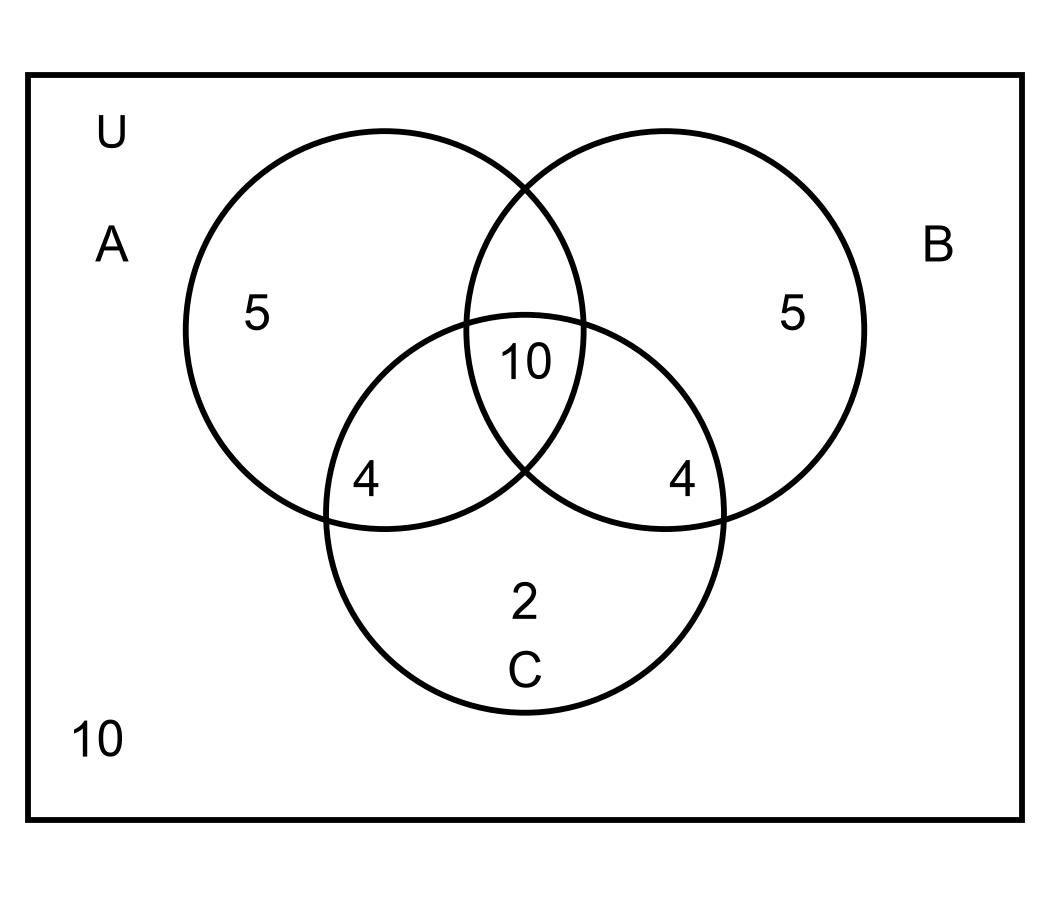
\includegraphics[width=0.38\textwidth]{figures/venn_50_ABC.png}
\end{center}
\step{所以单选物理、化学的人数至多 10 人.}
\step{所以至多选选择物理和化学这两门课程的学生人数至多 $10+10=20$ 人.}
\step{故选 C.}
\solend

\fi

\item 设 $k\geqslant 1,\,k\in\mathbb{N}$，已知集合 $M=\{1,2,3,4,5\}$，若集合 $N_1,N_2,\dots,N_k$ 是集合 $M$ 的 $k$ 个不同非空子集，且 $N_1\cup N_2\cup\dots\cup N_k\neq M$，则 $k$ 的最大值为\mbox{（\quad）.}

\keepwithprev
A. $15$\qquad B. $16$\qquad C. $31$\qquad D. $32$

\ans{A}

\ifanswer
\solbegin
\step{由 $N_1\cup N_2\cup\dots\cup N_k\neq M$ 得所有非空子集的并集缺少集合 $M$ 中至少一个元素.}
\step{假设缺少元素 1，则所有非空子集 $N_i$ 均不含元素 1，即 $N_i$ 是集合 $\{2,3,4,5\}$ 非空子集，集合 $\{2,3,4,5\}$ 的非空子集个数为 $2^4-1=15$，且这些子集 $N_i$ 的并集必不含 1，满足条件.}
\step{假设 $k\geqslant 16$，要满足所有非空子集的并集不等于集合 $M$，必须至少有一个集合 $M$ 中的元素不在任何一个子集中，否则并集就会等于 $M$.}
\step{设这个缺失的元素是 1，那么 $k$ 个非空集都不含元素 1，即每个子集都是集合 $\{2,3,4,5\}$ 的非空子集.}
\step{而集合 $\{2,3,4,5\}$ 只有 $2^4-1=15$ 个不同的非空子集，所以无法从中取出至少 16 个不同的非空子集.}
\step{因此假设不成立，$k$ 必须小于 16.}
\step{所以 $k$ 的最大值为 15，故选 A.}
\solend

\fi

% 注：原卷此题的差集记号是反斜杠 $A\setminus B$（本稿曾误作 $A\vee B$）；$C$ 的集合描述里原卷留了一条
%     待填横线“$x\in A\underline{\quad}B$”（选项按填入的符号分四种情形），本稿曾误作 $\vee\vee$。
%     2026-09-15 回原图核对时已按原卷改回。
\item 对于集合 $A$、$B$，定义 $A\setminus B=\{x\mid x\in A\text{ 且 }x\notin B\}$，则对于集合 $A=\{x\mid x=6n+5,\,n\in\mathbb{N}\}$，$B=\{y\mid y=3m+7,\,m\in\mathbb{N}\}$，$C=\{x\mid x\in A\underline{\hspace{4em}}B\text{ 且 }x<1000\}$，以下说法正确的是\mbox{（\quad）.}

\keepwithprev
A. 若在横线上填入“$\cap$”，则 $C$ 的真子集有 $2^{12}-1$ 个；

B. 若在横线上填入“$\cup$”，则 $C$ 中元素个数大于 250；

C. 若在横线上填入“$\setminus$”，则 $C$ 的非空真子集有 $2^{153}-2$ 个；

% 注：原卷选项 D 作“若在横线上填入“$\cup\complement_{\mathbb N}$”，则 $\complement_{\mathbb N}C$ 中元素个数为 13”；
%     本稿曾把 $\complement_{\mathbb N}$ 抄成 $\varnothing$、把 $\complement_{\mathbb N}C$ 抄成 $C\setminus C$，2026-09-15 回原图核对时已订正。
D. 若在横线上填入“$\cup\complement_{\mathbb{N}}$”，则 $\complement_{\mathbb{N}}C$ 中元素个数为 13.

\ans{B}

\ifanswer
\solbegin
\step{$x=6n+5=3(2n+1)+2$，$y=3m+7=3(m+2)+1$，集合 $A$、$B$ 无公共元素.}
\step{选项 A 中，集合 $C$ 为空集，没有真子集，$A$ 错；}
\step{选项 B 中，由 $6n+5<1000$ 得 $n<165\tfrac{5}{6}$，由 $3m+7<1000$ 得 $m<331$，因此 $C$ 中元素个数为 $166+331=497$，B 正确；}
\step{选项 C 中，$C$ 中元素个数为 166，非空真子集个数为 $2^{166}-2$，C 错；}
% 注：原卷此行作“$\complement_{\mathbb N}C=\complement_{\mathbb N}(A\cup\complement_{\mathbb N}B)
%     =\complement_{\mathbb N}A\cap\complement_{\mathbb N}(\complement_{\mathbb N}B)=\complement_{\mathbb N}A\cap B$，
%     而 $B\subseteq\complement_{\mathbb N}A$”；本稿曾把 $\complement_{\mathbb N}$ 抄成 $C\setminus$，同日已订正。
\step{选项 D 中，$\complement_{\mathbb{N}}C=\complement_{\mathbb{N}}(A\cup\complement_{\mathbb{N}}B)=\complement_{\mathbb{N}}A\cap\complement_{\mathbb{N}}(\complement_{\mathbb{N}}B)=\complement_{\mathbb{N}}A\cap B$，而 $B\subseteq\complement_{\mathbb{N}}A$.}
\step{因此其中元素个数为 331 个，D 错.}
\step{故选 B.}
\solend

\fi
\end{enumerate}

\bigsec{三、解答题}

\begin{enumerate}
\setcounter{enumi}{16}

\item 已知集合 $A=\{x\mid x<-1\text{ 或 }x>4\}$，$B=\{x\mid m+1\leqslant x\leqslant 2m+4\}$.
\begin{enumerate}[label=(\arabic*)]
\item 若 $m=2$，求 $A\cup B$ 和 $\left(\complement_{\R} A\right)\cap B$；
\item 若 $A\cap B=\varnothing$，求 $m$ 的取值范围.
\end{enumerate}

\ans{（1）$A\cup B=\{x\mid x<-1\text{ 或 }x\geqslant 3\}$，$\left(\complement_{\R} A\right)\cap B=\{x\mid 3\leqslant x\leqslant 4\}$；（2）$(-\infty,-3)\cup[-2,0]$}

\ifanswer
\solbegin
\stepm{(1)}{当 $m=2$ 时，集合 $B=\{x\mid 3\leqslant x\leqslant 8\}$.}
\step{又因为 $A=\{x\mid x<-1\text{ 或 }x>4\}$，则 $\complement_{\R}A=\{x\mid -1\leqslant x\leqslant 4\}$，所以 $A\cup B=\{x\mid x<-1\text{ 或 }x\geqslant 3\}$，$\left(\complement_{\R} A\right)\cap B=\{x\mid 3\leqslant x\leqslant 4\}$.}
\stepm{(2)}{因为 $A\cap B=\varnothing$，所以当 $B=\varnothing$ 时，$m+1>2m+4$，解得 $m<-3$ 满足题意；}
\step{当 $B\neq\varnothing$ 时，要满足题意，只需 $\begin{cases}m+1\leqslant 2m+4 \\ m+1\geqslant -1 \\ 2m+4\leqslant 4\end{cases}$，解得 $-2\leqslant m\leqslant 0$.}
\step{综上，实数 $m$ 的范围为 $m<-3$ 或 $-2\leqslant m\leqslant 0$，即 $(-\infty,-3)\cup[-2,0]$.}
\solend

\fi
\ansspace[6]
\item 设集合 $A=\{x\mid x^2+4x=0\}$，$B=\{x\mid x^2+2(a+1)x+a^2-1=0\}$.
\begin{enumerate}[label=(\arabic*)]
\item 写出集合 $A$ 的所有子集；
\item 若 $A\cap B=B$，求实数 $a$ 的取值范围.
\end{enumerate}

\ans{（1）$\{\varnothing,\{0\},\{-4\},\{0,-4\}\}$；（2）$a=1$ 或 $a\leqslant -1$}

\ifanswer
\solbegin
% 注：原卷此行印作“集合 $A$ 的所有子集为 $\varnothing,\{0\},\{-4\},\{0-4\}$”（末项漏逗号、且未加外层花括号）；
%     本稿按规范的列举写法给出，2026-09-15 回原图核对时加注。
\stepm{(1)}{由题意得 $A=\{0,-4\}$，集合 $A$ 的所有子集为 $\varnothing,\{0\},\{-4\},\{0,-4\}$.}
\stepm{(2)}{由 $A\cap B=B$ 得 $B\subseteq A$，所以 $B=\{0\}$ 或 $B=\{-4\}$ 或 $B=\{0,-4\}$ 或 $B=\varnothing$.}
\step{若 $B=\{0\}$ 时，$x^2+2(a+1)x+a^2-1=0$ 有两个相等的根 $0$，则 $\begin{cases}-2(a+1)=0 \\ a^2-1=-4\times(-4)\end{cases}$，解得 $a=-1$.}
\step{若 $B=\{-4\}$ 时，$x^2+2(a+1)x+a^2-1=0$ 有两个相等的根 $-4$，则 $\left\{\begin{matrix}-2(a+1)=-8 \\ a^2-1=-4\times(-4)\end{matrix}\right.$，$a$ 无解.}
\step{若 $B=\{0,-4\}$ 时，$x^2+2(a+1)x+a^2-1=0$ 有两个不相等的根 $0$ 和 $-4$，则 $\begin{cases}-2(a+1)=-4 \\ a^2-1=0\end{cases}$，解得 $a=1$.}
\step{当 $B=\varnothing$ 时，$x^2+2(a+1)x+a^2-1=0$ 无实数根，$\Delta=[2(a+1)]^2-4(a^2-1)=8a+8<0$，得 $a<-1$.}
\step{综上，$a=1$ 或 $a\leqslant -1$.}
\solend

\fi
\ansspace[6]
\item 已知集合 $A=\{x\mid x^2-5x+6=0\}$，$B=\{x\mid mx+1=0\}$，$C=\{x\in\mathbb{N}\mid \sqrt{x}\leqslant 1\}$，且 $A\cup B=A$.
\begin{enumerate}[label=(\arabic*)]
\item 求集合 $M=\{x\mid x\subseteq A\}$ 的真子集的个数；
\item 求实数 $m$ 的值组成的集合；
% 注：原卷本题的定义作“集合 $E=\{x\mid -x\in D,\,2-x^2\notin D\}$”；本稿曾把 $\notin$ 抄成 $\in$
%     （那样 $E=\varnothing$，与答案 $-5$ 冲突），2026-09-15 回原图核对时已订正。
\item 若集合 $D=A\cup C$，定义：集合 $E=\{x\mid -x\in D,\,2-x^2\notin D\}$，求集合 $E$ 中所有元素的和.
\end{enumerate}

\ans{（1）$15$；（2）$\left\{0,-\tfrac{1}{2},-\tfrac{1}{3}\right\}$；（3）$-5$}

\ifanswer
\solbegin
\stepm{(1)}{$A=\{x\mid x^2-5x+6=0\}=\{2,3\}$.}
\step{由 $M=\{x\mid x\subseteq A\}$ 得 $M$ 是 $A$ 的所有子集构成的集合，集合 $A$ 有 2 个元素，故 $A$ 的子集共 $2^2=4$ 个，即 $M$ 含 4 个元素，$M$ 的真子集个数为 $2^4-1=15$.}
\stepm{(2)}{由 (1) 得 $A=\{2,3\}$，集合 $B=\{x\mid mx+1=0\}$.}
\step{由 $A\cup B=A$ 得 $B\subseteq A$，分两种情况：① 当 $m=0$ 时，方程 $mx+1=0$ 无解，$B=\varnothing$，空集是任意集合的子集，符合条件；}
\stepm{②}{当 $m\neq 0$ 时，$B=\{-\tfrac{1}{m}\}$，由 $B\subseteq A$ 得 $-\tfrac{1}{m}=2$ 或 $-\tfrac{1}{m}=3$，解得 $m=-\tfrac{1}{2}$ 或 $m=-\tfrac{1}{3}$.}
\step{实数 $m$ 的取值集合为 $\left\{0,-\tfrac{1}{2},-\tfrac{1}{3}\right\}$.}
\stepm{(3)}{由 (1) 得 $A=\{2,3\}$.}
\step{由 $x\in\mathbb{N}$ 且 $\sqrt{x}\leqslant 1$，得 $x=0$ 或 $x=1$，故 $C=\{0,1\}$.}
\step{所以 $D=A\cup C=\{0,1,2,3\}$.}
\step{由 $-x\in D$ 得 $x$ 的候选值为 $0,-1,-2,-3$.}
\step{由于集合 $E=\{x\mid -x\in D,\,2-x^2\in D\}$，当 $x=0$ 时，$2-x^2=2\in D$，不符合题意；}
\step{当 $x=-1$ 时，$2-x^2=1\in D$，不符合题意；}
\step{当 $x=-2$ 时，$2-x^2=-2\notin D$，符合题意；}
\step{当 $x=-3$ 时，$2-x^2=-7\notin D$，符合题意.}
\step{故 $E=\{-2,-3\}$，所有元素的和为 $-2+(-3)=-5$.}
\solend

\fi
\ansspace[8]
\item 设集合 $M$ 是至少含有两个元素的数集，若 $M$ 中存在两个元素 $x$、$y$ 满足它们的积 $xy\in M$，则称 $M$ 为可积数集.
\begin{enumerate}[label=(\arabic*)]
\item 设集合 $A=\{2,3,5\}$，试判断 $A$ 是否为可积数集？并说明理由；
\item 设集合 $B=\{2,3,4,a\}$，若 $B$ 为可积数集，求实数 $a$ 的取值集合；
\item 设集合 $D=\{x\mid t<x<t+2\}$，若 $D$ 不是可积数集，求实数 $t$ 的取值范围.
\end{enumerate}

% 注：原卷本题【答案】与文末解析的结论都含 $\frac{3}{4}$；本稿曾漏掉 $\frac{3}{4}$
%     （与本稿自己的解析结论不一致），2026-09-15 回原图核对时已订正。
\ans{（1）否；（2）$\left\{0,\tfrac{1}{2},\tfrac{2}{3},\tfrac{3}{4},1,\tfrac{4}{3},\tfrac{3}{2},6,8,12\right\}$；（3）$t\in(-\infty,-2]\cup[2,+\infty)$}

\ifanswer
\solbegin
\stepm{(1)}{因为 $2\times 3=6\notin A$，$2\times 5=10\notin A$，$3\times 5=15\notin A$，所以 $A$ 中任意两个元素的积都不是 $A$ 中的元素，即 $A$ 不是可积数集.}
\stepm{(2)}{若 $B=\{2,3,4,a\}$ 为可积数集，则 $2\times 3=6\in B$，或 $2\times 4=8\in B$ 或 $3\times 4=12\in B$ 或 $2a\in B$ 或 $3a\in B$ 或 $4a\in B$.}
\step{若 $6\in B$，则 $a=6$；}
\step{若 $8\in B$，则 $a=8$；}
\step{若 $12\in B$，则 $a=12$；}
\step{若 $2a\in B$，则 $2a=2$ 或 $2a=3$ 或 $2a=4$ 或 $2a=a$，解得 $a=1$ 或 $a=\tfrac{3}{2}$ 或 $a=2$（舍）或 $a=0$；}
\step{若 $3a\in B$，则 $3a=2$ 或 $3a=3$ 或 $3a=4$ 或 $3a=a$，解得 $a=\tfrac{2}{3}$ 或 $a=1$ 或 $a=\tfrac{4}{3}$ 或 $a=0$；}
\step{若 $4a\in B$，则 $4a=2$ 或 $4a=3$ 或 $4a=4$ 或 $4a=a$，解得 $a=\tfrac{1}{2}$ 或 $a=\tfrac{3}{4}$ 或 $a=1$ 或 $a=0$.}
\step{综上，实数 $a$ 的取值集合为 $\left\{0,\tfrac{1}{2},\tfrac{2}{3},\tfrac{3}{4},1,\tfrac{4}{3},\tfrac{3}{2},6,8,12\right\}$.}
\stepm{(3)}{若 $D=\{x\mid t<x<t+2\}$ 不是可积数集，则 $\forall x,y\in(t,t+2)$，$xy\notin(t,t+2)$.}
\step{当 $t+2\leqslant 0$，即 $t\leqslant -2$ 时，$0\leqslant(t+2)^2<xy<t^2$，此时 $xy\notin D$，满足题意；}
\step{当 $t\geqslant 0$ 时，$0\leqslant t^2<xy<(t+2)^2$，因为 $(t+2)^2>t$，所以若 $xy\notin D$，则 $t^2\geqslant t+2$，即 $t^2-t-2\geqslant 0$，解得 $t\geqslant 2$ 或 $t\leqslant -1$，此时 $t\geqslant 2$ 满足题意；}
% 注：原卷此句作“当 $t<0<t+2$，即 $-2<t<0$ 时，$\exists x=0$，$xy=0\in D$，不满足题意，舍去”；
%     本稿曾把 $\in D$ 抄成 $\notin D$（$-2<t<0$ 时 $0\in(t,t+2)$，确有 $0\in D$），同日已订正。
\step{当 $t<0<t+2$，即 $-2<t<0$ 时，$\exists x=0$，$xy=0\in D$，不满足题意，舍去.}
\step{综上，所求实数 $t$ 的取值范围为 $t\geqslant 2$ 或 $t\leqslant -2$，故 $t\in(-\infty,-2]\cup[2,+\infty)$.}
\solend

\fi
\ansspace[8]
\ansneed{7cm}
\item 已知集合 $A$ 为非空数集，定义：$S=\{x\mid x=a+b,\,a,b\in A\}$，$T=\{x\mid x=|a-b|,a,b\in A\}$（实数 $a$、$b$ 可以相同）.
\begin{enumerate}[label=(\arabic*)]
\item 若集合 $A=\{2,5\}$，直接写出集合 $S$、$T$；
\item 若集合 $A=\{x_1,x_2,x_3,x_4\}$，$x_1<x_2<x_3<x_4$，且 $T=A$，求证：$x_1+x_4=x_3+x_2$；
\item 若集合 $A\subseteq\{x\mid 0\leqslant x\leqslant 2025,\,x\in\mathbb{N}\}$，$S\cap T=\varnothing$，记 $|A|$ 为集合 $A$ 中的元素个数，求 $|A|$ 的最大值.
\end{enumerate}

\ans{（1）$S=\{4,7,10\}$，$T=\{0,3\}$；（2）略；（3）$1350$}

\ifanswer
\solbegin
\stepm{(1)}{$S=\{4,7,10\}$，$T=\{0,3\}$.}
\stepm{(2)}{由集合 $A=\{x_1,x_2,x_3,x_4\}$，$x_1<x_2<x_3<x_4$，则 $T$ 集合的元素在 $0,x_2-x_1,x_3-x_1,x_4-x_1,x_3-x_2,x_4-x_2,x_4-x_3$ 中，且 $0<x_2-x_1<x_3-x_1<x_4-x_1$，$x_3-x_2<x_4-x_2<x_4-x_3$，因为 $A=T$，所以 $A$ 中最大元素 $x_4$ 必在 $T$ 中，而 $x_4-x_1$ 为 7 个元素中的最大者.}
\step{故 $x_4=x_4-x_1$，即 $x_1=0$.}
\step{故 $A=\{0,x_2,x_3,x_4\}$.}
\step{则 $x_3-x_2$、$x_4-x_2$、$x_4-x_3$ 与 $x_2$、$x_3$、$x_4$ 重复.}
\step{而 $0<x_3-x_2<x_3$，故 $x_3-x_2=x_2$，即 $x_3=2x_2$.}
% 注：原卷此句作“而 $0<x_4-x_3<x_4$，故 $x_4-x_3=x_2$ 或 $x_4-x_3=x_3$”；本稿曾把上界写成 $x_3$
%     （那样排除不了 $x_4-x_3=x_3$，与后半句自相矛盾），2026-09-15 回原图核对时已订正。
\step{而 $0<x_4-x_3<x_4$，故 $x_4-x_3=x_2$ 或 $x_4-x_3=x_3$.}
\step{若 $x_4=2x_3=4x_2$，则 $A=\{0,x_2,2x_2,4x_2\}$，$4x_2-x_2=3x_2\notin T$，与题设矛盾.}
\step{故 $x_4-x_3=x_2$，又因为 $x_1=0$，所以 $x_4+x_1=x_3+x_2$.}
% 注：原卷此行作“则 $2a_1<a_1+a_2<a_1+a_3<\cdots<a_1+a_k<a_2+a_k<a_3+a_k<\cdots<a_{k-1}+a_k<2a_k$，
%     所以 $|S|\geqslant 2k-1$，$a_1-a_1<a_2-a_1<a_3-a_1<\cdots<a_k-a_1$，所以 $|T|\geqslant k$”；
%     本稿曾把这个不等式链抄乱（作 $\cdots<a_1+a_k<a_2+a_3<a_k+a_k\leqslant 2a_k$）且把首项写成 $a_i-a_1$，
%     2026-09-15 回原图核对时已订正。
\stepm{(3)}{设 $A=\{a_1,a_2,\dots,a_k\}$ 满足题意，其中 $a_1<a_2<\dots<a_k$，则 $2a_1<a_1+a_2<a_1+a_3<\dots<a_1+a_k<a_2+a_k<a_3+a_k<\dots<a_{k-1}+a_k<2a_k$，所以 $|S|\geqslant 2k-1$，$a_1-a_1<a_2-a_1<a_3-a_1<\dots<a_k-a_1$，所以 $|T|\geqslant k$.}
\step{因为 $S\cap T=\varnothing$，由容斥原理得 $|S\cup T|=|S|+|T|\geqslant 3k-1$.}
\step{$S\cup T$ 中最小的元素为 0，最大的元素为 $2a_k$，$|S\cup T|\leqslant 2a_k+1$，所以 $3k-1\leqslant 2a_k+1\leqslant 2\times 2025+1\,(k\geqslant 1,k\in\mathbb{N})$，即 $3k-1\leqslant 4051$，解得 $k\leqslant 1350\tfrac{2}{3}$.}
\step{实际上 $A=\{676,677,678,\dots,2025\}$ 时满足题意，证明如下：设 $A=\{m,m+1,m+2,\dots,2025\}$，$m\in\mathbb{N}$.}
\step{则 $S=\{2m,2m+1,2m+2,\dots,4050\}$，$T=\{0,1,2,\dots,2025-m\}$.}
\step{由题意得 $2025-m<2m$，即 $m>675$.}
\step{所以 $A=\{676,677,678,\dots,2025\}$ 时满足题意，此时集合 $A$ 中的元素的个数最多.}
\step{综上所述，集合 $A$ 中元素的个数的最大值是 1350.}
\solend

\fi
\ansspace*[10]
\end{enumerate}

\end{document}"
% 紧凑版：xelatex "\def\iscompact{1}% 高一07_交附闵行_周练1.tex —— 高一上数学“2026-2027 年交附闵行高一上周练 1”（试卷版/答案版）
% 试卷版：xelatex 高一07_交附闵行_周练1.tex
% 答案版：xelatex "\def\isanswer{1}\input{高一07_交附闵行_周练1.tex}"
% 紧凑版：xelatex "\def\iscompact{1}\input{高一07_交附闵行_周练1.tex}"
%
% 原始材料是微信公众号图文（“魔都数学加油站”，作者署名“破晓”），正文为 11 张 PNG 页
% （1080×1527）；卷面上的粉色斜水印“魔都数学加油站”属水印，未录入。原文本身就是一份
% **讲评版**——题下直接印出【答案】或【解析】，本稿把这些答案与解析移到答案版，试卷版即
% 一张干净的空卷。
%
% 与原卷的排版差异（均已在 README“说明”中交代）：
%   ① 原文自**第 3 题**起（第 1、2 题未在该文发布），源码里以 \setcounter{enumi}{2} 起编；
%   ② 原卷本就印有分节标题“一、填空题”“二、选择题”“三、解答题”（已在原图上逐页放大
%      核对过），本稿照原卷分节，只把标题改排成全稿统一的“大节标题”样式；
%   ③ 原卷的实数集、整数集符号作正体 $R$（第 7 题）、$Z$（第 11 题），本稿按全稿惯例统一
%      写作 $\R$、$\Z$；
%   ④ 第 14 题【解析】里的 Venn 图取自原卷截图（`figures/venn_50_ABC.png`，4× LANCZOS
%      放大），未用 TikZ 重绘.

\documentclass[a4paper,11pt]{article}
\usepackage{common}

\begin{document}

\examtitlest{2026--2027 学年度交附闵行高一上周练 1}{集合与常用逻辑用语}

\bigsec{一、填空题}

\begin{enumerate}
\setcounter{enumi}{2}

\item 已知集合 $A=\{2,14,x^2+5\}$，$B=\{2,2x\}$，若 $A\cap B=B$，则实数 $x=$ \blankline[2em].

\ans{$7$}

\ifanswer
\solbegin
\step{因为 $A\cap B=B$，所以 $B\subseteq A$，所以 $2x=14$ 或 $x^2+5=2x$.}
\step{$2x=14$ 时，$x=7$，此时 $A=\{2,14,54\}$，$B=\{2,14\}$ 满足题意；}
\step{$x^2+5=2x$ 时，$(x-1)^2+4=0$，无解.}
\step{所以 $x=7$.}
\solend

\fi
\item 设集合 $A=\{y\mid y=x^2-1\}$，$B=\{(x,y)\mid y=x\}$，则 $A\cap B=$ \blankline[2em].

\ans{$\varnothing$}

\item 若集合 $\{0,-1,2a\}=\{a-1,-|a|,a+1\}$，实数 $a$ 的值为 \blankline[2em].

\ans{$\pm 1$}

\ifanswer
\solbegin
\step{令 $A=\{0,-1,2a\}$，$B=\{a-1,-|a|,a+1\}$，因为 $\{0,-1,2a\}=\{a-1,-|a|,a+1\}$，若 $a-1=0$，则 $a=1$，则 $A=\{0,-1,2\}$，$B=\{0,-1,2\}$，满足要求；}
\step{若 $-|a|=0$，则 $a=0$，则 $A=\{0,-1,0\}$，不满足集合元素的互异性；}
\step{若 $a+1=0$，则 $a=-1$，则 $A=\{0,-1,-2\}$，$B=\{0,-1,-2\}$，满足要求.}
\step{故实数 $a$ 的值为 $\pm 1$.}
\solend

\fi
\item 已知全集 $U=(-4,3]$，$A=\{x\in U\mid x^2+2x-8=0\}$，$B=\{x\in U\mid -3<1-2x\leqslant 5\}$，则 $\left(\complement_U B\right)\cap A=$ \blankline[2em].

\ans{$\{2\}$}

\item 已知集合 $A=\{x\mid 1-a\leqslant x\leqslant 1+a,\,a\in\R\}$ 中只有一个整数元素，则实数 $a$ 的取值范围为 \blankline[2em].

\ans{$[0,1)$}

\ifanswer
\solbegin
\step{集合 $A=\{x\mid 1-a\leqslant x\leqslant 1+a,\,a\in\R\}$ 中只有一个整数元素，则 $A\neq\varnothing,\,1-a\leqslant 1+a$，即 $a\geqslant 0$，此时 $1\in A$，故 $\begin{cases}1+a<2 \\ 1-a>0\end{cases}$，解得 $a<1$.}
\step{故 $a\in[0,1)$.}
\solend

\fi
\item 已知全集 $U=\{x\in\mathbb{N}\mid x\leqslant 9\}$，$A\cap B=\{3\}$，$\overline{A}\cap B=\{4,6,8\}$，$A\cap\overline{B}=\{1,5\}$，则 $\overline{A}=$ \blankline[2em].

\ans{$\{0,2,4,6,7,8,9\}$}

\ifanswer
\solbegin
\step{由题意得 $U=\{x\in\mathbb{N}\mid x\leqslant 9\}=\{0,1,2,3,4,5,6,7,8,9\}$，$A\cap B=\{3\}$ 得 $A$、$B$ 中含有元素 $3$；}
\step{$\overline{A}\cap B=\{4,6,8\}$ 得 $B$ 中含有 $4$、$6$、$8$，集合 $A$ 中不含 $4$、$6$、$8$；}
\step{$A\cap\overline{B}=\{1,5\}$ 得 $A$ 含有 $1$、$5$，集合 $B$ 不含 $1$、$5$.}
\step{对于 $0$，假设集合 $A$ 中含有 $0$，由 $A\cap B=\{3\}$ 得 $B$ 不含 $0$，则 $A\cap\overline{B}$ 必含元素 $0$，与 $A\cap\overline{B}=\{1,5\}$ 矛盾.}
\step{同理可得集合 $A$ 中不含元素 $2$、$7$、$9$.}
\step{综上所述，$A=\{1,3,5\}$.}
\step{故 $\overline{A}=\{0,2,4,6,7,8,9\}$.}
\solend

\fi
\item 已知一个有四个数字元素的集合 $S$，$S$ 的所有子集的元素和（空集的元素和认为是 0）的总和为 16208，则 $S$ 的元素之和等于 \blankline[2em].

\ans{$2026$}

\ifanswer
\solbegin
\step{设 $S=\{a_1,a_2,a_3,a_4\}$，$S$ 的每个元素在所有子集中均出现 $2^3$ 次，故 $(a_1+a_2+a_3+a_4)\cdot 2^3=16208$，所以 $a_1+a_2+a_3+a_4=2026$，故 $S$ 的元素之和等于 2026.}
\solend

\fi
\item 已知集合 $M=\{x\in\mathbb{N}\mid 1\leqslant x\leqslant 12\}$，集合 $A_1$、$A_2$、$A_3$ 满足：① 每个集合都恰有 4 个元素；② $A_1\cup A_2\cup A_3=M$. 集合 $A_i\,(i=1,2,3)$ 中元素的最大值与最小值之和称为集合 $A_i$ 的特征数，记为 $X_i\,(i=1,2,3)$，则 $X_1+X_2+X_3$ 的最大值与最小值的积为 \blankline[2em].

\ans{$1485$}

\ifanswer
\solbegin
\step{集合 $M=\{x\in\mathbb{N}\mid 1\leqslant x\leqslant 12\}$ 中最小值为 1，最大值为 12.}
% 注：原卷此处印作“则 $A_1=13$”（原卷笔误，按上下文应为 $X_1=13$），本稿按 $X_1$ 规范，2026-09-15 回原图核对时加注。
\stepm{①}{若使 $X_1+X_2+X_3$ 取得最大值，不妨设 $A_1=\{1,2,3,12\}$，则 $X_1=13$，则剩余的数中最小值是 4，最大值是 11，令 $A_2=\{4,5,6,11\}$，则 $X_2=15$，则 $A_3=\{7,8,9,10\}$，$X_3=17$，则 $X_1+X_2+X_3$ 的最大值为 $13+15+17=45$；}
\stepm{②}{若使 $X_1+X_2+X_3$ 取得最小值，则 $A_1=\{1,4,5,6\}$，则 $X_1=7$，令 $A_2=\{2,7,8,9\}$，则 $X_2=11$，则 $A_3=\{3,10,11,12\}$，$X_3=15$，则此时 $X_1+X_2+X_3$ 的最小值为 $7+11+15=33$.}
\step{故 $X_1+X_2+X_3$ 的最大值与最小值的积为 $45\times 33=1485$.}
\solend

\fi
\item 对于集合 $M=\{a\mid a=x^2-y^2,\,x\in\Z,\,y\in\Z\}$，给出如下三个结论：

① 如果 $P=\{b\mid b=2n+1,\,n\in\Z\}$，那么 $P\subseteq M$；

% 注：原卷此条作“如果 $c=4n+2$，$n\in\Z$，那么 $c\notin M$”；本稿曾把 $\notin$ 抄成 $\in$
%     （那样②为假，与本卷答案 ①②③ 冲突），2026-09-15 回原图核对时已订正。
② 如果 $c=4n+2$，$n\in\Z$，那么 $c\notin M$；

③ 如果 $a_1\in M$，$a_2\in M$，那么 $a_1a_2\in M$. 其中正确结论的序号是 \blankline[2em].

\ans{①②③}

\ifanswer
\solbegin
\stepm{①}{由已知 $b=2n+1,\,n\in\Z$，则恒有 $2n+1=(n+1)^2-n^2,\,n\in\Z$，所以 $2n+1\in M$，所以 $P\subseteq M$，所以①正确；}
\stepm{②}{元素 $c=4n+2,\,n\in\Z$，若 $4n+2\in M$，则存在 $x$、$y\in\Z$ 使得 $x^2-y^2=4n+2$，所以 $4n+2=(x+y)(x-y)$，则 $x+y$ 与 $x-y$ 同奇或同偶.}
\step{若 $x+y$ 与 $x-y$ 都是奇数，则 $(x+y)(x-y)$ 为奇数，而 $4n+2$ 是偶数；}
\step{若 $x+y$ 和 $x-y$ 都是偶数，则 $(x+y)(x-y)$ 能被 4 整除，而 $4n+2$ 不能被 4 整除.}
\step{所以 $4n+2\notin M$，即 $c\notin M$，故②正确；}
\stepm{③}{因为 $a_1$、$a_2\in M$，则 $a_1a_2$ 还是整数，所以 $a_1a_2\in M$，故③正确.}
\step{故正确的是①②③.}
\solend

\fi
\item 用 $C(A)$ 表示非空集合 $A$ 中的元素的个数，定义 $A*B=|C(A)-C(B)|$，若 $A=\{x\mid x^2-2024x-2025=0\}$，$B=\{x\mid (2x^2+ax)(x^2+2ax+6)=0\}$，若 $A*B=1$，则 $a$ 的所有可能取值构成集合 $M$，则 $C(M)=$ \blankline[2em].

\ans{$5$}

\ifanswer
\solbegin
\step{$x^2-2024x-2025=0$ 得 $x=2025$ 或 $x=-1$，即 $C(A)=2$，因为 $A*B=|C(A)-C(B)|=1$，所以 $C(B)=3$ 或 $C(B)=1$.}
\step{方程 $(2x^2+ax)(x^2+2ax+6)=0$ 化为 $x(2x+a)(x^2+2ax+6)=0$.}
\step{当 $a=0$ 时，方程化为 $2x^3(x^2+6)=0$，解得 $x=0$，所以 $B=\{0\}$，$C(B)=1$，符合题意.}
\step{当 $a\neq 0$ 时，方程化为 $x=0$ 或 $x=-\tfrac{a}{2}$ 或 $x^2+2ax+6=0$.}
\step{因为 $0\neq -\tfrac{a}{2}$，$C(B)\neq 1$，故只有 $C(B)=3$.}
\step{故 $x^2+2ax+6=0$ 有两个相等的非零实数根，所以 $\Delta=4a^2-4\times 6=0$，解得 $a=\pm\sqrt{6}$，符合题意.}
\step{当 $x^2+2ax+6=0$ 有两个不相等实根，设 $x_1$、$x_2$，若 $x_1=-\tfrac{a}{2}$，由韦达定理得 $\begin{cases}x_1+x_2=-2a \\ x_1x_2=6\end{cases}$，% 注：原卷作“得 $x_2=-\frac{3a}{2}$”（由 $x_1+x_2=-2a$、$x_1=-\frac{a}{2}$ 得 $x_2=-\frac{3a}{2}$）；
%     本稿曾漏掉负号，2026-09-15 回原图核对时已订正。
得 $x_2=-\tfrac{3a}{2}$，$-\tfrac{a}{2}\cdot(-\tfrac{3a}{2})=\tfrac{3a^2}{4}=6$，解得 $a=\pm 2\sqrt{2}$，符合题意.}
\step{综上所述，$M=\{0,\sqrt{6},-\sqrt{6},2\sqrt{2},-2\sqrt{2}\}$，所以 $C(M)=5$.}
\solend

\fi
\end{enumerate}

\bigsec{二、选择题}

\begin{enumerate}
\setcounter{enumi}{12}

\item 已知集合 $A=\{1,2,3,4,5\}$，$B=\{x\mid \tfrac{x-1}{2}\in\Z,\,x\in A\}$，则集合 $B$ 的真子集个数为\mbox{（\quad）.}

\keepwithprev
A. $3$\qquad B. $5$\qquad C. $7$\qquad D. $15$

\ans{C}

\ifanswer
\solbegin
\step{已知集合 $A=\{1,2,3,4,5\}$，$B=\{x\mid\tfrac{x-1}{2}\in\Z,\,x\in A\}$.}
\step{因为 $\tfrac{x-1}{2}\in\Z$，所以 $x$ 为奇数，所以 $B=\{1,3,5\}$.}
\step{所以集合 $B$ 中有 3 个元素，所以集合 $B$ 的真子集个数为 $2^3-1=7$.}
\step{故选 C.}
\solend

\fi

\item 高一二班共有学生 50 人，每名学生要从物理、化学、生物、历史、地理、政治这六门课程中选择三门课程进行学习. 已知选择物理、化学、生物的学生各有至少 20 人，这三门课程都不选的有 10 人，这三门课程都选的有 10 人，在这三门课程中选择任意两门课程的都至少有 14 人，物理、化学只选一科的学生都至少 5 人，那么选择物理和化学这两门课程的学生人数至多\mbox{（\quad）.}

\keepwithprev
A. $18$\qquad B. $19$\qquad C. $20$\qquad D. $21$

\ans{C}

\ifanswer
\solbegin
\step{可以把学生 50 人看作一个集合 $U$，选择物理的人数组成集合 $A$，选择化学的人数组成集合 $B$，选择生物的人数组成集合 $C$.}
\step{要使选择物理和化学这两门课程的学生人数最多，除这三门课程都不选的有 10 人，这三门课程都选的有 10 人，则其他科选择人数均为最少，因为物理、化学只选一科的学生都至少 5 人，即得到单选物理的最少 5 人，单选化学的最少 5 人.}
\step{因为在这三门课程中选择任意两门课程的都至少有 14 人，单选化学、生物的最少 4 人，单选物理、生物的最少 4 人.}
\step{因为选择物理、化学、生物的学生各有至少 20 人，所以单选生物的最少 2 人.}
\step{以上人数最少 30 人，可作出如图所示的韦恩图：}
% 注：原卷此处印有一张韦恩图（三个圆 $A$、$B$、$C$，$A$ 独有 5、$B$ 独有 5、三集合公共 10、
%     $A\cap C$ 独有 4、$B\cap C$ 独有 4、$C$ 独有 2、三集合之外 10）；本稿此前漏排此图而正文仍作
%     “如图”，2026-09-15 回原图核对时按原卷截图补入（见 figures/venn_50_ABC.png）。
\begin{center}
% 插图取自原卷截图（裁去截图残影后 4× LANCZOS 放大），不用 TikZ 手绘
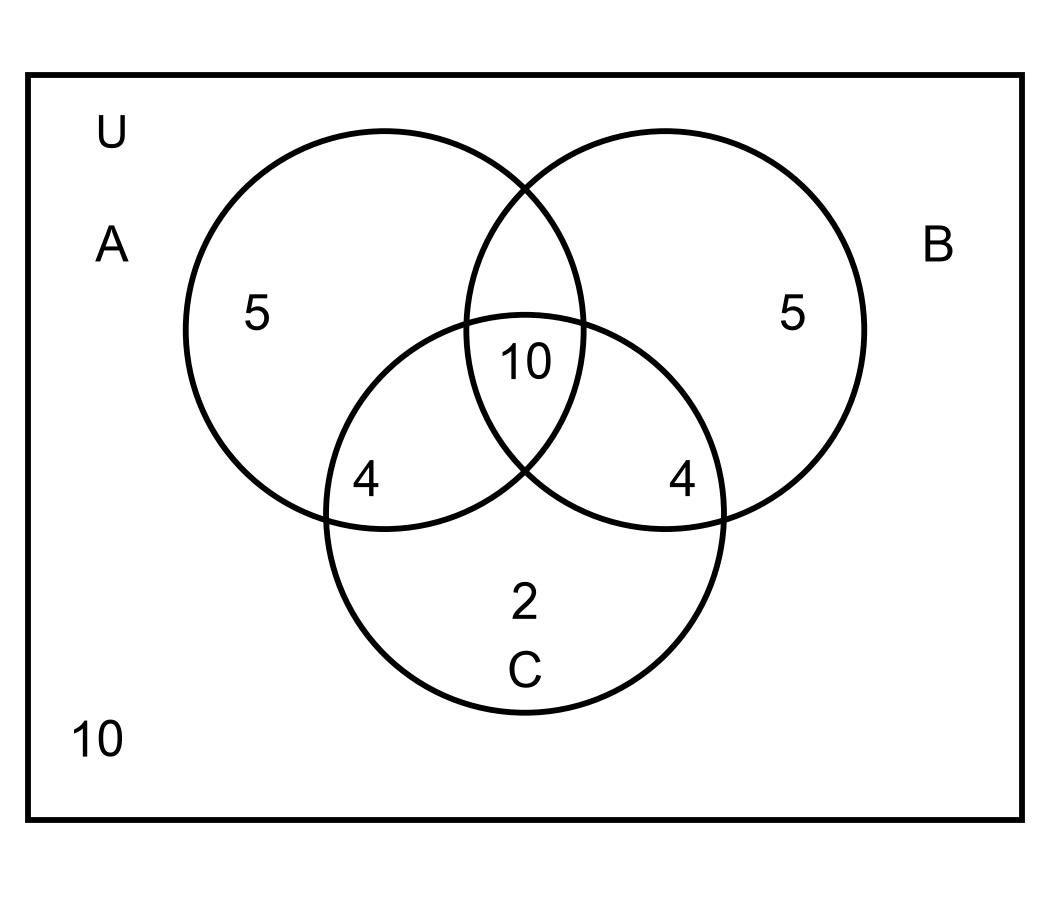
\includegraphics[width=0.38\textwidth]{figures/venn_50_ABC.png}
\end{center}
\step{所以单选物理、化学的人数至多 10 人.}
\step{所以至多选选择物理和化学这两门课程的学生人数至多 $10+10=20$ 人.}
\step{故选 C.}
\solend

\fi

\item 设 $k\geqslant 1,\,k\in\mathbb{N}$，已知集合 $M=\{1,2,3,4,5\}$，若集合 $N_1,N_2,\dots,N_k$ 是集合 $M$ 的 $k$ 个不同非空子集，且 $N_1\cup N_2\cup\dots\cup N_k\neq M$，则 $k$ 的最大值为\mbox{（\quad）.}

\keepwithprev
A. $15$\qquad B. $16$\qquad C. $31$\qquad D. $32$

\ans{A}

\ifanswer
\solbegin
\step{由 $N_1\cup N_2\cup\dots\cup N_k\neq M$ 得所有非空子集的并集缺少集合 $M$ 中至少一个元素.}
\step{假设缺少元素 1，则所有非空子集 $N_i$ 均不含元素 1，即 $N_i$ 是集合 $\{2,3,4,5\}$ 非空子集，集合 $\{2,3,4,5\}$ 的非空子集个数为 $2^4-1=15$，且这些子集 $N_i$ 的并集必不含 1，满足条件.}
\step{假设 $k\geqslant 16$，要满足所有非空子集的并集不等于集合 $M$，必须至少有一个集合 $M$ 中的元素不在任何一个子集中，否则并集就会等于 $M$.}
\step{设这个缺失的元素是 1，那么 $k$ 个非空集都不含元素 1，即每个子集都是集合 $\{2,3,4,5\}$ 的非空子集.}
\step{而集合 $\{2,3,4,5\}$ 只有 $2^4-1=15$ 个不同的非空子集，所以无法从中取出至少 16 个不同的非空子集.}
\step{因此假设不成立，$k$ 必须小于 16.}
\step{所以 $k$ 的最大值为 15，故选 A.}
\solend

\fi

% 注：原卷此题的差集记号是反斜杠 $A\setminus B$（本稿曾误作 $A\vee B$）；$C$ 的集合描述里原卷留了一条
%     待填横线“$x\in A\underline{\quad}B$”（选项按填入的符号分四种情形），本稿曾误作 $\vee\vee$。
%     2026-09-15 回原图核对时已按原卷改回。
\item 对于集合 $A$、$B$，定义 $A\setminus B=\{x\mid x\in A\text{ 且 }x\notin B\}$，则对于集合 $A=\{x\mid x=6n+5,\,n\in\mathbb{N}\}$，$B=\{y\mid y=3m+7,\,m\in\mathbb{N}\}$，$C=\{x\mid x\in A\underline{\hspace{4em}}B\text{ 且 }x<1000\}$，以下说法正确的是\mbox{（\quad）.}

\keepwithprev
A. 若在横线上填入“$\cap$”，则 $C$ 的真子集有 $2^{12}-1$ 个；

B. 若在横线上填入“$\cup$”，则 $C$ 中元素个数大于 250；

C. 若在横线上填入“$\setminus$”，则 $C$ 的非空真子集有 $2^{153}-2$ 个；

% 注：原卷选项 D 作“若在横线上填入“$\cup\complement_{\mathbb N}$”，则 $\complement_{\mathbb N}C$ 中元素个数为 13”；
%     本稿曾把 $\complement_{\mathbb N}$ 抄成 $\varnothing$、把 $\complement_{\mathbb N}C$ 抄成 $C\setminus C$，2026-09-15 回原图核对时已订正。
D. 若在横线上填入“$\cup\complement_{\mathbb{N}}$”，则 $\complement_{\mathbb{N}}C$ 中元素个数为 13.

\ans{B}

\ifanswer
\solbegin
\step{$x=6n+5=3(2n+1)+2$，$y=3m+7=3(m+2)+1$，集合 $A$、$B$ 无公共元素.}
\step{选项 A 中，集合 $C$ 为空集，没有真子集，$A$ 错；}
\step{选项 B 中，由 $6n+5<1000$ 得 $n<165\tfrac{5}{6}$，由 $3m+7<1000$ 得 $m<331$，因此 $C$ 中元素个数为 $166+331=497$，B 正确；}
\step{选项 C 中，$C$ 中元素个数为 166，非空真子集个数为 $2^{166}-2$，C 错；}
% 注：原卷此行作“$\complement_{\mathbb N}C=\complement_{\mathbb N}(A\cup\complement_{\mathbb N}B)
%     =\complement_{\mathbb N}A\cap\complement_{\mathbb N}(\complement_{\mathbb N}B)=\complement_{\mathbb N}A\cap B$，
%     而 $B\subseteq\complement_{\mathbb N}A$”；本稿曾把 $\complement_{\mathbb N}$ 抄成 $C\setminus$，同日已订正。
\step{选项 D 中，$\complement_{\mathbb{N}}C=\complement_{\mathbb{N}}(A\cup\complement_{\mathbb{N}}B)=\complement_{\mathbb{N}}A\cap\complement_{\mathbb{N}}(\complement_{\mathbb{N}}B)=\complement_{\mathbb{N}}A\cap B$，而 $B\subseteq\complement_{\mathbb{N}}A$.}
\step{因此其中元素个数为 331 个，D 错.}
\step{故选 B.}
\solend

\fi
\end{enumerate}

\bigsec{三、解答题}

\begin{enumerate}
\setcounter{enumi}{16}

\item 已知集合 $A=\{x\mid x<-1\text{ 或 }x>4\}$，$B=\{x\mid m+1\leqslant x\leqslant 2m+4\}$.
\begin{enumerate}[label=(\arabic*)]
\item 若 $m=2$，求 $A\cup B$ 和 $\left(\complement_{\R} A\right)\cap B$；
\item 若 $A\cap B=\varnothing$，求 $m$ 的取值范围.
\end{enumerate}

\ans{（1）$A\cup B=\{x\mid x<-1\text{ 或 }x\geqslant 3\}$，$\left(\complement_{\R} A\right)\cap B=\{x\mid 3\leqslant x\leqslant 4\}$；（2）$(-\infty,-3)\cup[-2,0]$}

\ifanswer
\solbegin
\stepm{(1)}{当 $m=2$ 时，集合 $B=\{x\mid 3\leqslant x\leqslant 8\}$.}
\step{又因为 $A=\{x\mid x<-1\text{ 或 }x>4\}$，则 $\complement_{\R}A=\{x\mid -1\leqslant x\leqslant 4\}$，所以 $A\cup B=\{x\mid x<-1\text{ 或 }x\geqslant 3\}$，$\left(\complement_{\R} A\right)\cap B=\{x\mid 3\leqslant x\leqslant 4\}$.}
\stepm{(2)}{因为 $A\cap B=\varnothing$，所以当 $B=\varnothing$ 时，$m+1>2m+4$，解得 $m<-3$ 满足题意；}
\step{当 $B\neq\varnothing$ 时，要满足题意，只需 $\begin{cases}m+1\leqslant 2m+4 \\ m+1\geqslant -1 \\ 2m+4\leqslant 4\end{cases}$，解得 $-2\leqslant m\leqslant 0$.}
\step{综上，实数 $m$ 的范围为 $m<-3$ 或 $-2\leqslant m\leqslant 0$，即 $(-\infty,-3)\cup[-2,0]$.}
\solend

\fi
\ansspace[6]
\item 设集合 $A=\{x\mid x^2+4x=0\}$，$B=\{x\mid x^2+2(a+1)x+a^2-1=0\}$.
\begin{enumerate}[label=(\arabic*)]
\item 写出集合 $A$ 的所有子集；
\item 若 $A\cap B=B$，求实数 $a$ 的取值范围.
\end{enumerate}

\ans{（1）$\{\varnothing,\{0\},\{-4\},\{0,-4\}\}$；（2）$a=1$ 或 $a\leqslant -1$}

\ifanswer
\solbegin
% 注：原卷此行印作“集合 $A$ 的所有子集为 $\varnothing,\{0\},\{-4\},\{0-4\}$”（末项漏逗号、且未加外层花括号）；
%     本稿按规范的列举写法给出，2026-09-15 回原图核对时加注。
\stepm{(1)}{由题意得 $A=\{0,-4\}$，集合 $A$ 的所有子集为 $\varnothing,\{0\},\{-4\},\{0,-4\}$.}
\stepm{(2)}{由 $A\cap B=B$ 得 $B\subseteq A$，所以 $B=\{0\}$ 或 $B=\{-4\}$ 或 $B=\{0,-4\}$ 或 $B=\varnothing$.}
\step{若 $B=\{0\}$ 时，$x^2+2(a+1)x+a^2-1=0$ 有两个相等的根 $0$，则 $\begin{cases}-2(a+1)=0 \\ a^2-1=-4\times(-4)\end{cases}$，解得 $a=-1$.}
\step{若 $B=\{-4\}$ 时，$x^2+2(a+1)x+a^2-1=0$ 有两个相等的根 $-4$，则 $\left\{\begin{matrix}-2(a+1)=-8 \\ a^2-1=-4\times(-4)\end{matrix}\right.$，$a$ 无解.}
\step{若 $B=\{0,-4\}$ 时，$x^2+2(a+1)x+a^2-1=0$ 有两个不相等的根 $0$ 和 $-4$，则 $\begin{cases}-2(a+1)=-4 \\ a^2-1=0\end{cases}$，解得 $a=1$.}
\step{当 $B=\varnothing$ 时，$x^2+2(a+1)x+a^2-1=0$ 无实数根，$\Delta=[2(a+1)]^2-4(a^2-1)=8a+8<0$，得 $a<-1$.}
\step{综上，$a=1$ 或 $a\leqslant -1$.}
\solend

\fi
\ansspace[6]
\item 已知集合 $A=\{x\mid x^2-5x+6=0\}$，$B=\{x\mid mx+1=0\}$，$C=\{x\in\mathbb{N}\mid \sqrt{x}\leqslant 1\}$，且 $A\cup B=A$.
\begin{enumerate}[label=(\arabic*)]
\item 求集合 $M=\{x\mid x\subseteq A\}$ 的真子集的个数；
\item 求实数 $m$ 的值组成的集合；
% 注：原卷本题的定义作“集合 $E=\{x\mid -x\in D,\,2-x^2\notin D\}$”；本稿曾把 $\notin$ 抄成 $\in$
%     （那样 $E=\varnothing$，与答案 $-5$ 冲突），2026-09-15 回原图核对时已订正。
\item 若集合 $D=A\cup C$，定义：集合 $E=\{x\mid -x\in D,\,2-x^2\notin D\}$，求集合 $E$ 中所有元素的和.
\end{enumerate}

\ans{（1）$15$；（2）$\left\{0,-\tfrac{1}{2},-\tfrac{1}{3}\right\}$；（3）$-5$}

\ifanswer
\solbegin
\stepm{(1)}{$A=\{x\mid x^2-5x+6=0\}=\{2,3\}$.}
\step{由 $M=\{x\mid x\subseteq A\}$ 得 $M$ 是 $A$ 的所有子集构成的集合，集合 $A$ 有 2 个元素，故 $A$ 的子集共 $2^2=4$ 个，即 $M$ 含 4 个元素，$M$ 的真子集个数为 $2^4-1=15$.}
\stepm{(2)}{由 (1) 得 $A=\{2,3\}$，集合 $B=\{x\mid mx+1=0\}$.}
\step{由 $A\cup B=A$ 得 $B\subseteq A$，分两种情况：① 当 $m=0$ 时，方程 $mx+1=0$ 无解，$B=\varnothing$，空集是任意集合的子集，符合条件；}
\stepm{②}{当 $m\neq 0$ 时，$B=\{-\tfrac{1}{m}\}$，由 $B\subseteq A$ 得 $-\tfrac{1}{m}=2$ 或 $-\tfrac{1}{m}=3$，解得 $m=-\tfrac{1}{2}$ 或 $m=-\tfrac{1}{3}$.}
\step{实数 $m$ 的取值集合为 $\left\{0,-\tfrac{1}{2},-\tfrac{1}{3}\right\}$.}
\stepm{(3)}{由 (1) 得 $A=\{2,3\}$.}
\step{由 $x\in\mathbb{N}$ 且 $\sqrt{x}\leqslant 1$，得 $x=0$ 或 $x=1$，故 $C=\{0,1\}$.}
\step{所以 $D=A\cup C=\{0,1,2,3\}$.}
\step{由 $-x\in D$ 得 $x$ 的候选值为 $0,-1,-2,-3$.}
\step{由于集合 $E=\{x\mid -x\in D,\,2-x^2\in D\}$，当 $x=0$ 时，$2-x^2=2\in D$，不符合题意；}
\step{当 $x=-1$ 时，$2-x^2=1\in D$，不符合题意；}
\step{当 $x=-2$ 时，$2-x^2=-2\notin D$，符合题意；}
\step{当 $x=-3$ 时，$2-x^2=-7\notin D$，符合题意.}
\step{故 $E=\{-2,-3\}$，所有元素的和为 $-2+(-3)=-5$.}
\solend

\fi
\ansspace[8]
\item 设集合 $M$ 是至少含有两个元素的数集，若 $M$ 中存在两个元素 $x$、$y$ 满足它们的积 $xy\in M$，则称 $M$ 为可积数集.
\begin{enumerate}[label=(\arabic*)]
\item 设集合 $A=\{2,3,5\}$，试判断 $A$ 是否为可积数集？并说明理由；
\item 设集合 $B=\{2,3,4,a\}$，若 $B$ 为可积数集，求实数 $a$ 的取值集合；
\item 设集合 $D=\{x\mid t<x<t+2\}$，若 $D$ 不是可积数集，求实数 $t$ 的取值范围.
\end{enumerate}

% 注：原卷本题【答案】与文末解析的结论都含 $\frac{3}{4}$；本稿曾漏掉 $\frac{3}{4}$
%     （与本稿自己的解析结论不一致），2026-09-15 回原图核对时已订正。
\ans{（1）否；（2）$\left\{0,\tfrac{1}{2},\tfrac{2}{3},\tfrac{3}{4},1,\tfrac{4}{3},\tfrac{3}{2},6,8,12\right\}$；（3）$t\in(-\infty,-2]\cup[2,+\infty)$}

\ifanswer
\solbegin
\stepm{(1)}{因为 $2\times 3=6\notin A$，$2\times 5=10\notin A$，$3\times 5=15\notin A$，所以 $A$ 中任意两个元素的积都不是 $A$ 中的元素，即 $A$ 不是可积数集.}
\stepm{(2)}{若 $B=\{2,3,4,a\}$ 为可积数集，则 $2\times 3=6\in B$，或 $2\times 4=8\in B$ 或 $3\times 4=12\in B$ 或 $2a\in B$ 或 $3a\in B$ 或 $4a\in B$.}
\step{若 $6\in B$，则 $a=6$；}
\step{若 $8\in B$，则 $a=8$；}
\step{若 $12\in B$，则 $a=12$；}
\step{若 $2a\in B$，则 $2a=2$ 或 $2a=3$ 或 $2a=4$ 或 $2a=a$，解得 $a=1$ 或 $a=\tfrac{3}{2}$ 或 $a=2$（舍）或 $a=0$；}
\step{若 $3a\in B$，则 $3a=2$ 或 $3a=3$ 或 $3a=4$ 或 $3a=a$，解得 $a=\tfrac{2}{3}$ 或 $a=1$ 或 $a=\tfrac{4}{3}$ 或 $a=0$；}
\step{若 $4a\in B$，则 $4a=2$ 或 $4a=3$ 或 $4a=4$ 或 $4a=a$，解得 $a=\tfrac{1}{2}$ 或 $a=\tfrac{3}{4}$ 或 $a=1$ 或 $a=0$.}
\step{综上，实数 $a$ 的取值集合为 $\left\{0,\tfrac{1}{2},\tfrac{2}{3},\tfrac{3}{4},1,\tfrac{4}{3},\tfrac{3}{2},6,8,12\right\}$.}
\stepm{(3)}{若 $D=\{x\mid t<x<t+2\}$ 不是可积数集，则 $\forall x,y\in(t,t+2)$，$xy\notin(t,t+2)$.}
\step{当 $t+2\leqslant 0$，即 $t\leqslant -2$ 时，$0\leqslant(t+2)^2<xy<t^2$，此时 $xy\notin D$，满足题意；}
\step{当 $t\geqslant 0$ 时，$0\leqslant t^2<xy<(t+2)^2$，因为 $(t+2)^2>t$，所以若 $xy\notin D$，则 $t^2\geqslant t+2$，即 $t^2-t-2\geqslant 0$，解得 $t\geqslant 2$ 或 $t\leqslant -1$，此时 $t\geqslant 2$ 满足题意；}
% 注：原卷此句作“当 $t<0<t+2$，即 $-2<t<0$ 时，$\exists x=0$，$xy=0\in D$，不满足题意，舍去”；
%     本稿曾把 $\in D$ 抄成 $\notin D$（$-2<t<0$ 时 $0\in(t,t+2)$，确有 $0\in D$），同日已订正。
\step{当 $t<0<t+2$，即 $-2<t<0$ 时，$\exists x=0$，$xy=0\in D$，不满足题意，舍去.}
\step{综上，所求实数 $t$ 的取值范围为 $t\geqslant 2$ 或 $t\leqslant -2$，故 $t\in(-\infty,-2]\cup[2,+\infty)$.}
\solend

\fi
\ansspace[8]
\ansneed{7cm}
\item 已知集合 $A$ 为非空数集，定义：$S=\{x\mid x=a+b,\,a,b\in A\}$，$T=\{x\mid x=|a-b|,a,b\in A\}$（实数 $a$、$b$ 可以相同）.
\begin{enumerate}[label=(\arabic*)]
\item 若集合 $A=\{2,5\}$，直接写出集合 $S$、$T$；
\item 若集合 $A=\{x_1,x_2,x_3,x_4\}$，$x_1<x_2<x_3<x_4$，且 $T=A$，求证：$x_1+x_4=x_3+x_2$；
\item 若集合 $A\subseteq\{x\mid 0\leqslant x\leqslant 2025,\,x\in\mathbb{N}\}$，$S\cap T=\varnothing$，记 $|A|$ 为集合 $A$ 中的元素个数，求 $|A|$ 的最大值.
\end{enumerate}

\ans{（1）$S=\{4,7,10\}$，$T=\{0,3\}$；（2）略；（3）$1350$}

\ifanswer
\solbegin
\stepm{(1)}{$S=\{4,7,10\}$，$T=\{0,3\}$.}
\stepm{(2)}{由集合 $A=\{x_1,x_2,x_3,x_4\}$，$x_1<x_2<x_3<x_4$，则 $T$ 集合的元素在 $0,x_2-x_1,x_3-x_1,x_4-x_1,x_3-x_2,x_4-x_2,x_4-x_3$ 中，且 $0<x_2-x_1<x_3-x_1<x_4-x_1$，$x_3-x_2<x_4-x_2<x_4-x_3$，因为 $A=T$，所以 $A$ 中最大元素 $x_4$ 必在 $T$ 中，而 $x_4-x_1$ 为 7 个元素中的最大者.}
\step{故 $x_4=x_4-x_1$，即 $x_1=0$.}
\step{故 $A=\{0,x_2,x_3,x_4\}$.}
\step{则 $x_3-x_2$、$x_4-x_2$、$x_4-x_3$ 与 $x_2$、$x_3$、$x_4$ 重复.}
\step{而 $0<x_3-x_2<x_3$，故 $x_3-x_2=x_2$，即 $x_3=2x_2$.}
% 注：原卷此句作“而 $0<x_4-x_3<x_4$，故 $x_4-x_3=x_2$ 或 $x_4-x_3=x_3$”；本稿曾把上界写成 $x_3$
%     （那样排除不了 $x_4-x_3=x_3$，与后半句自相矛盾），2026-09-15 回原图核对时已订正。
\step{而 $0<x_4-x_3<x_4$，故 $x_4-x_3=x_2$ 或 $x_4-x_3=x_3$.}
\step{若 $x_4=2x_3=4x_2$，则 $A=\{0,x_2,2x_2,4x_2\}$，$4x_2-x_2=3x_2\notin T$，与题设矛盾.}
\step{故 $x_4-x_3=x_2$，又因为 $x_1=0$，所以 $x_4+x_1=x_3+x_2$.}
% 注：原卷此行作“则 $2a_1<a_1+a_2<a_1+a_3<\cdots<a_1+a_k<a_2+a_k<a_3+a_k<\cdots<a_{k-1}+a_k<2a_k$，
%     所以 $|S|\geqslant 2k-1$，$a_1-a_1<a_2-a_1<a_3-a_1<\cdots<a_k-a_1$，所以 $|T|\geqslant k$”；
%     本稿曾把这个不等式链抄乱（作 $\cdots<a_1+a_k<a_2+a_3<a_k+a_k\leqslant 2a_k$）且把首项写成 $a_i-a_1$，
%     2026-09-15 回原图核对时已订正。
\stepm{(3)}{设 $A=\{a_1,a_2,\dots,a_k\}$ 满足题意，其中 $a_1<a_2<\dots<a_k$，则 $2a_1<a_1+a_2<a_1+a_3<\dots<a_1+a_k<a_2+a_k<a_3+a_k<\dots<a_{k-1}+a_k<2a_k$，所以 $|S|\geqslant 2k-1$，$a_1-a_1<a_2-a_1<a_3-a_1<\dots<a_k-a_1$，所以 $|T|\geqslant k$.}
\step{因为 $S\cap T=\varnothing$，由容斥原理得 $|S\cup T|=|S|+|T|\geqslant 3k-1$.}
\step{$S\cup T$ 中最小的元素为 0，最大的元素为 $2a_k$，$|S\cup T|\leqslant 2a_k+1$，所以 $3k-1\leqslant 2a_k+1\leqslant 2\times 2025+1\,(k\geqslant 1,k\in\mathbb{N})$，即 $3k-1\leqslant 4051$，解得 $k\leqslant 1350\tfrac{2}{3}$.}
\step{实际上 $A=\{676,677,678,\dots,2025\}$ 时满足题意，证明如下：设 $A=\{m,m+1,m+2,\dots,2025\}$，$m\in\mathbb{N}$.}
\step{则 $S=\{2m,2m+1,2m+2,\dots,4050\}$，$T=\{0,1,2,\dots,2025-m\}$.}
\step{由题意得 $2025-m<2m$，即 $m>675$.}
\step{所以 $A=\{676,677,678,\dots,2025\}$ 时满足题意，此时集合 $A$ 中的元素的个数最多.}
\step{综上所述，集合 $A$ 中元素的个数的最大值是 1350.}
\solend

\fi
\ansspace*[10]
\end{enumerate}

\end{document}"
%
% 原始材料是微信公众号图文（“魔都数学加油站”，作者署名“破晓”），正文为 11 张 PNG 页
% （1080×1527）；卷面上的粉色斜水印“魔都数学加油站”属水印，未录入。原文本身就是一份
% **讲评版**——题下直接印出【答案】或【解析】，本稿把这些答案与解析移到答案版，试卷版即
% 一张干净的空卷。
%
% 与原卷的排版差异（均已在 README“说明”中交代）：
%   ① 原文自**第 3 题**起（第 1、2 题未在该文发布），源码里以 \setcounter{enumi}{2} 起编；
%   ② 原卷本就印有分节标题“一、填空题”“二、选择题”“三、解答题”（已在原图上逐页放大
%      核对过），本稿照原卷分节，只把标题改排成全稿统一的“大节标题”样式；
%   ③ 原卷的实数集、整数集符号作正体 $R$（第 7 题）、$Z$（第 11 题），本稿按全稿惯例统一
%      写作 $\R$、$\Z$；
%   ④ 第 14 题【解析】里的 Venn 图取自原卷截图（`figures/venn_50_ABC.png`，4× LANCZOS
%      放大），未用 TikZ 重绘.

\documentclass[a4paper,11pt]{article}
\usepackage{common}

\begin{document}

\examtitlest{2026--2027 学年度交附闵行高一上周练 1}{集合与常用逻辑用语}

\bigsec{一、填空题}

\begin{enumerate}
\setcounter{enumi}{2}

\item 已知集合 $A=\{2,14,x^2+5\}$，$B=\{2,2x\}$，若 $A\cap B=B$，则实数 $x=$ \blankline[2em].

\ans{$7$}

\ifanswer
\solbegin
\step{因为 $A\cap B=B$，所以 $B\subseteq A$，所以 $2x=14$ 或 $x^2+5=2x$.}
\step{$2x=14$ 时，$x=7$，此时 $A=\{2,14,54\}$，$B=\{2,14\}$ 满足题意；}
\step{$x^2+5=2x$ 时，$(x-1)^2+4=0$，无解.}
\step{所以 $x=7$.}
\solend

\fi
\item 设集合 $A=\{y\mid y=x^2-1\}$，$B=\{(x,y)\mid y=x\}$，则 $A\cap B=$ \blankline[2em].

\ans{$\varnothing$}

\item 若集合 $\{0,-1,2a\}=\{a-1,-|a|,a+1\}$，实数 $a$ 的值为 \blankline[2em].

\ans{$\pm 1$}

\ifanswer
\solbegin
\step{令 $A=\{0,-1,2a\}$，$B=\{a-1,-|a|,a+1\}$，因为 $\{0,-1,2a\}=\{a-1,-|a|,a+1\}$，若 $a-1=0$，则 $a=1$，则 $A=\{0,-1,2\}$，$B=\{0,-1,2\}$，满足要求；}
\step{若 $-|a|=0$，则 $a=0$，则 $A=\{0,-1,0\}$，不满足集合元素的互异性；}
\step{若 $a+1=0$，则 $a=-1$，则 $A=\{0,-1,-2\}$，$B=\{0,-1,-2\}$，满足要求.}
\step{故实数 $a$ 的值为 $\pm 1$.}
\solend

\fi
\item 已知全集 $U=(-4,3]$，$A=\{x\in U\mid x^2+2x-8=0\}$，$B=\{x\in U\mid -3<1-2x\leqslant 5\}$，则 $\left(\complement_U B\right)\cap A=$ \blankline[2em].

\ans{$\{2\}$}

\item 已知集合 $A=\{x\mid 1-a\leqslant x\leqslant 1+a,\,a\in\R\}$ 中只有一个整数元素，则实数 $a$ 的取值范围为 \blankline[2em].

\ans{$[0,1)$}

\ifanswer
\solbegin
\step{集合 $A=\{x\mid 1-a\leqslant x\leqslant 1+a,\,a\in\R\}$ 中只有一个整数元素，则 $A\neq\varnothing,\,1-a\leqslant 1+a$，即 $a\geqslant 0$，此时 $1\in A$，故 $\begin{cases}1+a<2 \\ 1-a>0\end{cases}$，解得 $a<1$.}
\step{故 $a\in[0,1)$.}
\solend

\fi
\item 已知全集 $U=\{x\in\mathbb{N}\mid x\leqslant 9\}$，$A\cap B=\{3\}$，$\overline{A}\cap B=\{4,6,8\}$，$A\cap\overline{B}=\{1,5\}$，则 $\overline{A}=$ \blankline[2em].

\ans{$\{0,2,4,6,7,8,9\}$}

\ifanswer
\solbegin
\step{由题意得 $U=\{x\in\mathbb{N}\mid x\leqslant 9\}=\{0,1,2,3,4,5,6,7,8,9\}$，$A\cap B=\{3\}$ 得 $A$、$B$ 中含有元素 $3$；}
\step{$\overline{A}\cap B=\{4,6,8\}$ 得 $B$ 中含有 $4$、$6$、$8$，集合 $A$ 中不含 $4$、$6$、$8$；}
\step{$A\cap\overline{B}=\{1,5\}$ 得 $A$ 含有 $1$、$5$，集合 $B$ 不含 $1$、$5$.}
\step{对于 $0$，假设集合 $A$ 中含有 $0$，由 $A\cap B=\{3\}$ 得 $B$ 不含 $0$，则 $A\cap\overline{B}$ 必含元素 $0$，与 $A\cap\overline{B}=\{1,5\}$ 矛盾.}
\step{同理可得集合 $A$ 中不含元素 $2$、$7$、$9$.}
\step{综上所述，$A=\{1,3,5\}$.}
\step{故 $\overline{A}=\{0,2,4,6,7,8,9\}$.}
\solend

\fi
\item 已知一个有四个数字元素的集合 $S$，$S$ 的所有子集的元素和（空集的元素和认为是 0）的总和为 16208，则 $S$ 的元素之和等于 \blankline[2em].

\ans{$2026$}

\ifanswer
\solbegin
\step{设 $S=\{a_1,a_2,a_3,a_4\}$，$S$ 的每个元素在所有子集中均出现 $2^3$ 次，故 $(a_1+a_2+a_3+a_4)\cdot 2^3=16208$，所以 $a_1+a_2+a_3+a_4=2026$，故 $S$ 的元素之和等于 2026.}
\solend

\fi
\item 已知集合 $M=\{x\in\mathbb{N}\mid 1\leqslant x\leqslant 12\}$，集合 $A_1$、$A_2$、$A_3$ 满足：① 每个集合都恰有 4 个元素；② $A_1\cup A_2\cup A_3=M$. 集合 $A_i\,(i=1,2,3)$ 中元素的最大值与最小值之和称为集合 $A_i$ 的特征数，记为 $X_i\,(i=1,2,3)$，则 $X_1+X_2+X_3$ 的最大值与最小值的积为 \blankline[2em].

\ans{$1485$}

\ifanswer
\solbegin
\step{集合 $M=\{x\in\mathbb{N}\mid 1\leqslant x\leqslant 12\}$ 中最小值为 1，最大值为 12.}
% 注：原卷此处印作“则 $A_1=13$”（原卷笔误，按上下文应为 $X_1=13$），本稿按 $X_1$ 规范，2026-09-15 回原图核对时加注。
\stepm{①}{若使 $X_1+X_2+X_3$ 取得最大值，不妨设 $A_1=\{1,2,3,12\}$，则 $X_1=13$，则剩余的数中最小值是 4，最大值是 11，令 $A_2=\{4,5,6,11\}$，则 $X_2=15$，则 $A_3=\{7,8,9,10\}$，$X_3=17$，则 $X_1+X_2+X_3$ 的最大值为 $13+15+17=45$；}
\stepm{②}{若使 $X_1+X_2+X_3$ 取得最小值，则 $A_1=\{1,4,5,6\}$，则 $X_1=7$，令 $A_2=\{2,7,8,9\}$，则 $X_2=11$，则 $A_3=\{3,10,11,12\}$，$X_3=15$，则此时 $X_1+X_2+X_3$ 的最小值为 $7+11+15=33$.}
\step{故 $X_1+X_2+X_3$ 的最大值与最小值的积为 $45\times 33=1485$.}
\solend

\fi
\item 对于集合 $M=\{a\mid a=x^2-y^2,\,x\in\Z,\,y\in\Z\}$，给出如下三个结论：

① 如果 $P=\{b\mid b=2n+1,\,n\in\Z\}$，那么 $P\subseteq M$；

% 注：原卷此条作“如果 $c=4n+2$，$n\in\Z$，那么 $c\notin M$”；本稿曾把 $\notin$ 抄成 $\in$
%     （那样②为假，与本卷答案 ①②③ 冲突），2026-09-15 回原图核对时已订正。
② 如果 $c=4n+2$，$n\in\Z$，那么 $c\notin M$；

③ 如果 $a_1\in M$，$a_2\in M$，那么 $a_1a_2\in M$. 其中正确结论的序号是 \blankline[2em].

\ans{①②③}

\ifanswer
\solbegin
\stepm{①}{由已知 $b=2n+1,\,n\in\Z$，则恒有 $2n+1=(n+1)^2-n^2,\,n\in\Z$，所以 $2n+1\in M$，所以 $P\subseteq M$，所以①正确；}
\stepm{②}{元素 $c=4n+2,\,n\in\Z$，若 $4n+2\in M$，则存在 $x$、$y\in\Z$ 使得 $x^2-y^2=4n+2$，所以 $4n+2=(x+y)(x-y)$，则 $x+y$ 与 $x-y$ 同奇或同偶.}
\step{若 $x+y$ 与 $x-y$ 都是奇数，则 $(x+y)(x-y)$ 为奇数，而 $4n+2$ 是偶数；}
\step{若 $x+y$ 和 $x-y$ 都是偶数，则 $(x+y)(x-y)$ 能被 4 整除，而 $4n+2$ 不能被 4 整除.}
\step{所以 $4n+2\notin M$，即 $c\notin M$，故②正确；}
\stepm{③}{因为 $a_1$、$a_2\in M$，则 $a_1a_2$ 还是整数，所以 $a_1a_2\in M$，故③正确.}
\step{故正确的是①②③.}
\solend

\fi
\item 用 $C(A)$ 表示非空集合 $A$ 中的元素的个数，定义 $A*B=|C(A)-C(B)|$，若 $A=\{x\mid x^2-2024x-2025=0\}$，$B=\{x\mid (2x^2+ax)(x^2+2ax+6)=0\}$，若 $A*B=1$，则 $a$ 的所有可能取值构成集合 $M$，则 $C(M)=$ \blankline[2em].

\ans{$5$}

\ifanswer
\solbegin
\step{$x^2-2024x-2025=0$ 得 $x=2025$ 或 $x=-1$，即 $C(A)=2$，因为 $A*B=|C(A)-C(B)|=1$，所以 $C(B)=3$ 或 $C(B)=1$.}
\step{方程 $(2x^2+ax)(x^2+2ax+6)=0$ 化为 $x(2x+a)(x^2+2ax+6)=0$.}
\step{当 $a=0$ 时，方程化为 $2x^3(x^2+6)=0$，解得 $x=0$，所以 $B=\{0\}$，$C(B)=1$，符合题意.}
\step{当 $a\neq 0$ 时，方程化为 $x=0$ 或 $x=-\tfrac{a}{2}$ 或 $x^2+2ax+6=0$.}
\step{因为 $0\neq -\tfrac{a}{2}$，$C(B)\neq 1$，故只有 $C(B)=3$.}
\step{故 $x^2+2ax+6=0$ 有两个相等的非零实数根，所以 $\Delta=4a^2-4\times 6=0$，解得 $a=\pm\sqrt{6}$，符合题意.}
\step{当 $x^2+2ax+6=0$ 有两个不相等实根，设 $x_1$、$x_2$，若 $x_1=-\tfrac{a}{2}$，由韦达定理得 $\begin{cases}x_1+x_2=-2a \\ x_1x_2=6\end{cases}$，% 注：原卷作“得 $x_2=-\frac{3a}{2}$”（由 $x_1+x_2=-2a$、$x_1=-\frac{a}{2}$ 得 $x_2=-\frac{3a}{2}$）；
%     本稿曾漏掉负号，2026-09-15 回原图核对时已订正。
得 $x_2=-\tfrac{3a}{2}$，$-\tfrac{a}{2}\cdot(-\tfrac{3a}{2})=\tfrac{3a^2}{4}=6$，解得 $a=\pm 2\sqrt{2}$，符合题意.}
\step{综上所述，$M=\{0,\sqrt{6},-\sqrt{6},2\sqrt{2},-2\sqrt{2}\}$，所以 $C(M)=5$.}
\solend

\fi
\end{enumerate}

\bigsec{二、选择题}

\begin{enumerate}
\setcounter{enumi}{12}

\item 已知集合 $A=\{1,2,3,4,5\}$，$B=\{x\mid \tfrac{x-1}{2}\in\Z,\,x\in A\}$，则集合 $B$ 的真子集个数为\mbox{（\quad）.}

\keepwithprev
A. $3$\qquad B. $5$\qquad C. $7$\qquad D. $15$

\ans{C}

\ifanswer
\solbegin
\step{已知集合 $A=\{1,2,3,4,5\}$，$B=\{x\mid\tfrac{x-1}{2}\in\Z,\,x\in A\}$.}
\step{因为 $\tfrac{x-1}{2}\in\Z$，所以 $x$ 为奇数，所以 $B=\{1,3,5\}$.}
\step{所以集合 $B$ 中有 3 个元素，所以集合 $B$ 的真子集个数为 $2^3-1=7$.}
\step{故选 C.}
\solend

\fi

\item 高一二班共有学生 50 人，每名学生要从物理、化学、生物、历史、地理、政治这六门课程中选择三门课程进行学习. 已知选择物理、化学、生物的学生各有至少 20 人，这三门课程都不选的有 10 人，这三门课程都选的有 10 人，在这三门课程中选择任意两门课程的都至少有 14 人，物理、化学只选一科的学生都至少 5 人，那么选择物理和化学这两门课程的学生人数至多\mbox{（\quad）.}

\keepwithprev
A. $18$\qquad B. $19$\qquad C. $20$\qquad D. $21$

\ans{C}

\ifanswer
\solbegin
\step{可以把学生 50 人看作一个集合 $U$，选择物理的人数组成集合 $A$，选择化学的人数组成集合 $B$，选择生物的人数组成集合 $C$.}
\step{要使选择物理和化学这两门课程的学生人数最多，除这三门课程都不选的有 10 人，这三门课程都选的有 10 人，则其他科选择人数均为最少，因为物理、化学只选一科的学生都至少 5 人，即得到单选物理的最少 5 人，单选化学的最少 5 人.}
\step{因为在这三门课程中选择任意两门课程的都至少有 14 人，单选化学、生物的最少 4 人，单选物理、生物的最少 4 人.}
\step{因为选择物理、化学、生物的学生各有至少 20 人，所以单选生物的最少 2 人.}
\step{以上人数最少 30 人，可作出如图所示的韦恩图：}
% 注：原卷此处印有一张韦恩图（三个圆 $A$、$B$、$C$，$A$ 独有 5、$B$ 独有 5、三集合公共 10、
%     $A\cap C$ 独有 4、$B\cap C$ 独有 4、$C$ 独有 2、三集合之外 10）；本稿此前漏排此图而正文仍作
%     “如图”，2026-09-15 回原图核对时按原卷截图补入（见 figures/venn_50_ABC.png）。
\begin{center}
% 插图取自原卷截图（裁去截图残影后 4× LANCZOS 放大），不用 TikZ 手绘
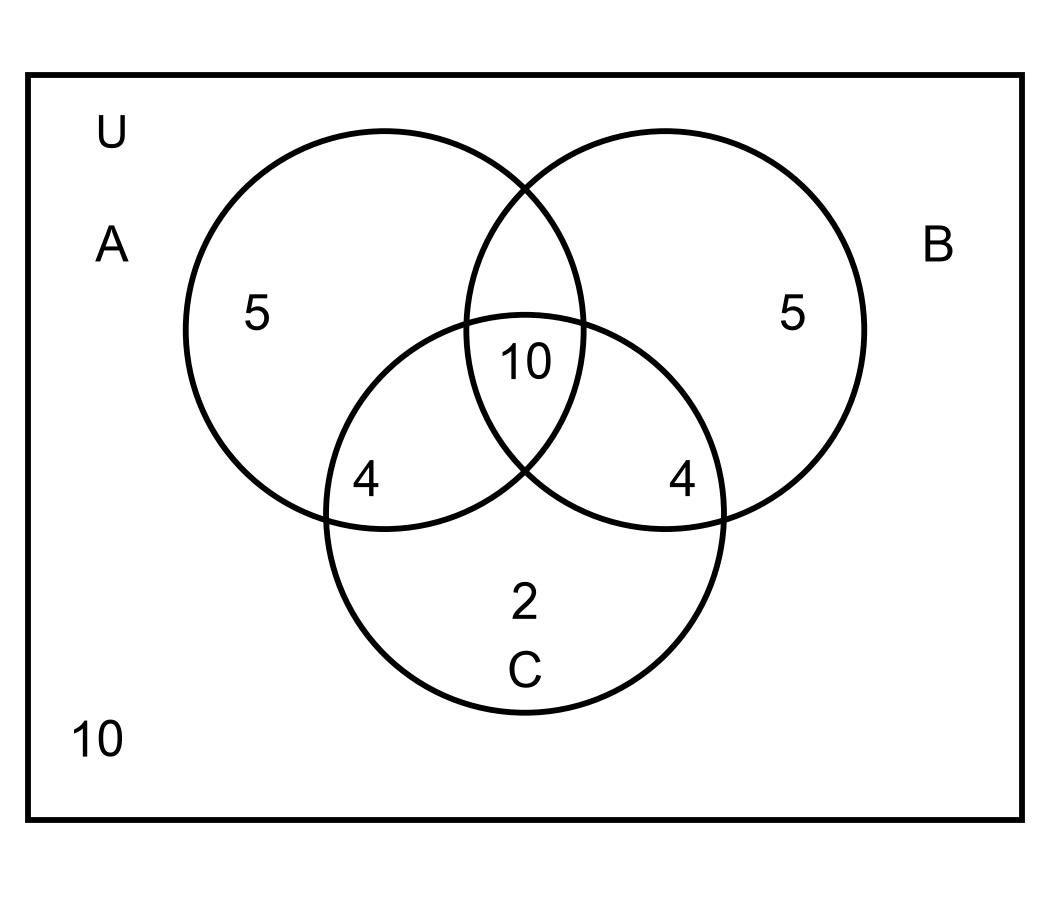
\includegraphics[width=0.38\textwidth]{figures/venn_50_ABC.png}
\end{center}
\step{所以单选物理、化学的人数至多 10 人.}
\step{所以至多选选择物理和化学这两门课程的学生人数至多 $10+10=20$ 人.}
\step{故选 C.}
\solend

\fi

\item 设 $k\geqslant 1,\,k\in\mathbb{N}$，已知集合 $M=\{1,2,3,4,5\}$，若集合 $N_1,N_2,\dots,N_k$ 是集合 $M$ 的 $k$ 个不同非空子集，且 $N_1\cup N_2\cup\dots\cup N_k\neq M$，则 $k$ 的最大值为\mbox{（\quad）.}

\keepwithprev
A. $15$\qquad B. $16$\qquad C. $31$\qquad D. $32$

\ans{A}

\ifanswer
\solbegin
\step{由 $N_1\cup N_2\cup\dots\cup N_k\neq M$ 得所有非空子集的并集缺少集合 $M$ 中至少一个元素.}
\step{假设缺少元素 1，则所有非空子集 $N_i$ 均不含元素 1，即 $N_i$ 是集合 $\{2,3,4,5\}$ 非空子集，集合 $\{2,3,4,5\}$ 的非空子集个数为 $2^4-1=15$，且这些子集 $N_i$ 的并集必不含 1，满足条件.}
\step{假设 $k\geqslant 16$，要满足所有非空子集的并集不等于集合 $M$，必须至少有一个集合 $M$ 中的元素不在任何一个子集中，否则并集就会等于 $M$.}
\step{设这个缺失的元素是 1，那么 $k$ 个非空集都不含元素 1，即每个子集都是集合 $\{2,3,4,5\}$ 的非空子集.}
\step{而集合 $\{2,3,4,5\}$ 只有 $2^4-1=15$ 个不同的非空子集，所以无法从中取出至少 16 个不同的非空子集.}
\step{因此假设不成立，$k$ 必须小于 16.}
\step{所以 $k$ 的最大值为 15，故选 A.}
\solend

\fi

% 注：原卷此题的差集记号是反斜杠 $A\setminus B$（本稿曾误作 $A\vee B$）；$C$ 的集合描述里原卷留了一条
%     待填横线“$x\in A\underline{\quad}B$”（选项按填入的符号分四种情形），本稿曾误作 $\vee\vee$。
%     2026-09-15 回原图核对时已按原卷改回。
\item 对于集合 $A$、$B$，定义 $A\setminus B=\{x\mid x\in A\text{ 且 }x\notin B\}$，则对于集合 $A=\{x\mid x=6n+5,\,n\in\mathbb{N}\}$，$B=\{y\mid y=3m+7,\,m\in\mathbb{N}\}$，$C=\{x\mid x\in A\underline{\hspace{4em}}B\text{ 且 }x<1000\}$，以下说法正确的是\mbox{（\quad）.}

\keepwithprev
A. 若在横线上填入“$\cap$”，则 $C$ 的真子集有 $2^{12}-1$ 个；

B. 若在横线上填入“$\cup$”，则 $C$ 中元素个数大于 250；

C. 若在横线上填入“$\setminus$”，则 $C$ 的非空真子集有 $2^{153}-2$ 个；

% 注：原卷选项 D 作“若在横线上填入“$\cup\complement_{\mathbb N}$”，则 $\complement_{\mathbb N}C$ 中元素个数为 13”；
%     本稿曾把 $\complement_{\mathbb N}$ 抄成 $\varnothing$、把 $\complement_{\mathbb N}C$ 抄成 $C\setminus C$，2026-09-15 回原图核对时已订正。
D. 若在横线上填入“$\cup\complement_{\mathbb{N}}$”，则 $\complement_{\mathbb{N}}C$ 中元素个数为 13.

\ans{B}

\ifanswer
\solbegin
\step{$x=6n+5=3(2n+1)+2$，$y=3m+7=3(m+2)+1$，集合 $A$、$B$ 无公共元素.}
\step{选项 A 中，集合 $C$ 为空集，没有真子集，$A$ 错；}
\step{选项 B 中，由 $6n+5<1000$ 得 $n<165\tfrac{5}{6}$，由 $3m+7<1000$ 得 $m<331$，因此 $C$ 中元素个数为 $166+331=497$，B 正确；}
\step{选项 C 中，$C$ 中元素个数为 166，非空真子集个数为 $2^{166}-2$，C 错；}
% 注：原卷此行作“$\complement_{\mathbb N}C=\complement_{\mathbb N}(A\cup\complement_{\mathbb N}B)
%     =\complement_{\mathbb N}A\cap\complement_{\mathbb N}(\complement_{\mathbb N}B)=\complement_{\mathbb N}A\cap B$，
%     而 $B\subseteq\complement_{\mathbb N}A$”；本稿曾把 $\complement_{\mathbb N}$ 抄成 $C\setminus$，同日已订正。
\step{选项 D 中，$\complement_{\mathbb{N}}C=\complement_{\mathbb{N}}(A\cup\complement_{\mathbb{N}}B)=\complement_{\mathbb{N}}A\cap\complement_{\mathbb{N}}(\complement_{\mathbb{N}}B)=\complement_{\mathbb{N}}A\cap B$，而 $B\subseteq\complement_{\mathbb{N}}A$.}
\step{因此其中元素个数为 331 个，D 错.}
\step{故选 B.}
\solend

\fi
\end{enumerate}

\bigsec{三、解答题}

\begin{enumerate}
\setcounter{enumi}{16}

\item 已知集合 $A=\{x\mid x<-1\text{ 或 }x>4\}$，$B=\{x\mid m+1\leqslant x\leqslant 2m+4\}$.
\begin{enumerate}[label=(\arabic*)]
\item 若 $m=2$，求 $A\cup B$ 和 $\left(\complement_{\R} A\right)\cap B$；
\item 若 $A\cap B=\varnothing$，求 $m$ 的取值范围.
\end{enumerate}

\ans{（1）$A\cup B=\{x\mid x<-1\text{ 或 }x\geqslant 3\}$，$\left(\complement_{\R} A\right)\cap B=\{x\mid 3\leqslant x\leqslant 4\}$；（2）$(-\infty,-3)\cup[-2,0]$}

\ifanswer
\solbegin
\stepm{(1)}{当 $m=2$ 时，集合 $B=\{x\mid 3\leqslant x\leqslant 8\}$.}
\step{又因为 $A=\{x\mid x<-1\text{ 或 }x>4\}$，则 $\complement_{\R}A=\{x\mid -1\leqslant x\leqslant 4\}$，所以 $A\cup B=\{x\mid x<-1\text{ 或 }x\geqslant 3\}$，$\left(\complement_{\R} A\right)\cap B=\{x\mid 3\leqslant x\leqslant 4\}$.}
\stepm{(2)}{因为 $A\cap B=\varnothing$，所以当 $B=\varnothing$ 时，$m+1>2m+4$，解得 $m<-3$ 满足题意；}
\step{当 $B\neq\varnothing$ 时，要满足题意，只需 $\begin{cases}m+1\leqslant 2m+4 \\ m+1\geqslant -1 \\ 2m+4\leqslant 4\end{cases}$，解得 $-2\leqslant m\leqslant 0$.}
\step{综上，实数 $m$ 的范围为 $m<-3$ 或 $-2\leqslant m\leqslant 0$，即 $(-\infty,-3)\cup[-2,0]$.}
\solend

\fi
\ansspace[6]
\item 设集合 $A=\{x\mid x^2+4x=0\}$，$B=\{x\mid x^2+2(a+1)x+a^2-1=0\}$.
\begin{enumerate}[label=(\arabic*)]
\item 写出集合 $A$ 的所有子集；
\item 若 $A\cap B=B$，求实数 $a$ 的取值范围.
\end{enumerate}

\ans{（1）$\{\varnothing,\{0\},\{-4\},\{0,-4\}\}$；（2）$a=1$ 或 $a\leqslant -1$}

\ifanswer
\solbegin
% 注：原卷此行印作“集合 $A$ 的所有子集为 $\varnothing,\{0\},\{-4\},\{0-4\}$”（末项漏逗号、且未加外层花括号）；
%     本稿按规范的列举写法给出，2026-09-15 回原图核对时加注。
\stepm{(1)}{由题意得 $A=\{0,-4\}$，集合 $A$ 的所有子集为 $\varnothing,\{0\},\{-4\},\{0,-4\}$.}
\stepm{(2)}{由 $A\cap B=B$ 得 $B\subseteq A$，所以 $B=\{0\}$ 或 $B=\{-4\}$ 或 $B=\{0,-4\}$ 或 $B=\varnothing$.}
\step{若 $B=\{0\}$ 时，$x^2+2(a+1)x+a^2-1=0$ 有两个相等的根 $0$，则 $\begin{cases}-2(a+1)=0 \\ a^2-1=-4\times(-4)\end{cases}$，解得 $a=-1$.}
\step{若 $B=\{-4\}$ 时，$x^2+2(a+1)x+a^2-1=0$ 有两个相等的根 $-4$，则 $\left\{\begin{matrix}-2(a+1)=-8 \\ a^2-1=-4\times(-4)\end{matrix}\right.$，$a$ 无解.}
\step{若 $B=\{0,-4\}$ 时，$x^2+2(a+1)x+a^2-1=0$ 有两个不相等的根 $0$ 和 $-4$，则 $\begin{cases}-2(a+1)=-4 \\ a^2-1=0\end{cases}$，解得 $a=1$.}
\step{当 $B=\varnothing$ 时，$x^2+2(a+1)x+a^2-1=0$ 无实数根，$\Delta=[2(a+1)]^2-4(a^2-1)=8a+8<0$，得 $a<-1$.}
\step{综上，$a=1$ 或 $a\leqslant -1$.}
\solend

\fi
\ansspace[6]
\item 已知集合 $A=\{x\mid x^2-5x+6=0\}$，$B=\{x\mid mx+1=0\}$，$C=\{x\in\mathbb{N}\mid \sqrt{x}\leqslant 1\}$，且 $A\cup B=A$.
\begin{enumerate}[label=(\arabic*)]
\item 求集合 $M=\{x\mid x\subseteq A\}$ 的真子集的个数；
\item 求实数 $m$ 的值组成的集合；
% 注：原卷本题的定义作“集合 $E=\{x\mid -x\in D,\,2-x^2\notin D\}$”；本稿曾把 $\notin$ 抄成 $\in$
%     （那样 $E=\varnothing$，与答案 $-5$ 冲突），2026-09-15 回原图核对时已订正。
\item 若集合 $D=A\cup C$，定义：集合 $E=\{x\mid -x\in D,\,2-x^2\notin D\}$，求集合 $E$ 中所有元素的和.
\end{enumerate}

\ans{（1）$15$；（2）$\left\{0,-\tfrac{1}{2},-\tfrac{1}{3}\right\}$；（3）$-5$}

\ifanswer
\solbegin
\stepm{(1)}{$A=\{x\mid x^2-5x+6=0\}=\{2,3\}$.}
\step{由 $M=\{x\mid x\subseteq A\}$ 得 $M$ 是 $A$ 的所有子集构成的集合，集合 $A$ 有 2 个元素，故 $A$ 的子集共 $2^2=4$ 个，即 $M$ 含 4 个元素，$M$ 的真子集个数为 $2^4-1=15$.}
\stepm{(2)}{由 (1) 得 $A=\{2,3\}$，集合 $B=\{x\mid mx+1=0\}$.}
\step{由 $A\cup B=A$ 得 $B\subseteq A$，分两种情况：① 当 $m=0$ 时，方程 $mx+1=0$ 无解，$B=\varnothing$，空集是任意集合的子集，符合条件；}
\stepm{②}{当 $m\neq 0$ 时，$B=\{-\tfrac{1}{m}\}$，由 $B\subseteq A$ 得 $-\tfrac{1}{m}=2$ 或 $-\tfrac{1}{m}=3$，解得 $m=-\tfrac{1}{2}$ 或 $m=-\tfrac{1}{3}$.}
\step{实数 $m$ 的取值集合为 $\left\{0,-\tfrac{1}{2},-\tfrac{1}{3}\right\}$.}
\stepm{(3)}{由 (1) 得 $A=\{2,3\}$.}
\step{由 $x\in\mathbb{N}$ 且 $\sqrt{x}\leqslant 1$，得 $x=0$ 或 $x=1$，故 $C=\{0,1\}$.}
\step{所以 $D=A\cup C=\{0,1,2,3\}$.}
\step{由 $-x\in D$ 得 $x$ 的候选值为 $0,-1,-2,-3$.}
\step{由于集合 $E=\{x\mid -x\in D,\,2-x^2\in D\}$，当 $x=0$ 时，$2-x^2=2\in D$，不符合题意；}
\step{当 $x=-1$ 时，$2-x^2=1\in D$，不符合题意；}
\step{当 $x=-2$ 时，$2-x^2=-2\notin D$，符合题意；}
\step{当 $x=-3$ 时，$2-x^2=-7\notin D$，符合题意.}
\step{故 $E=\{-2,-3\}$，所有元素的和为 $-2+(-3)=-5$.}
\solend

\fi
\ansspace[8]
\item 设集合 $M$ 是至少含有两个元素的数集，若 $M$ 中存在两个元素 $x$、$y$ 满足它们的积 $xy\in M$，则称 $M$ 为可积数集.
\begin{enumerate}[label=(\arabic*)]
\item 设集合 $A=\{2,3,5\}$，试判断 $A$ 是否为可积数集？并说明理由；
\item 设集合 $B=\{2,3,4,a\}$，若 $B$ 为可积数集，求实数 $a$ 的取值集合；
\item 设集合 $D=\{x\mid t<x<t+2\}$，若 $D$ 不是可积数集，求实数 $t$ 的取值范围.
\end{enumerate}

% 注：原卷本题【答案】与文末解析的结论都含 $\frac{3}{4}$；本稿曾漏掉 $\frac{3}{4}$
%     （与本稿自己的解析结论不一致），2026-09-15 回原图核对时已订正。
\ans{（1）否；（2）$\left\{0,\tfrac{1}{2},\tfrac{2}{3},\tfrac{3}{4},1,\tfrac{4}{3},\tfrac{3}{2},6,8,12\right\}$；（3）$t\in(-\infty,-2]\cup[2,+\infty)$}

\ifanswer
\solbegin
\stepm{(1)}{因为 $2\times 3=6\notin A$，$2\times 5=10\notin A$，$3\times 5=15\notin A$，所以 $A$ 中任意两个元素的积都不是 $A$ 中的元素，即 $A$ 不是可积数集.}
\stepm{(2)}{若 $B=\{2,3,4,a\}$ 为可积数集，则 $2\times 3=6\in B$，或 $2\times 4=8\in B$ 或 $3\times 4=12\in B$ 或 $2a\in B$ 或 $3a\in B$ 或 $4a\in B$.}
\step{若 $6\in B$，则 $a=6$；}
\step{若 $8\in B$，则 $a=8$；}
\step{若 $12\in B$，则 $a=12$；}
\step{若 $2a\in B$，则 $2a=2$ 或 $2a=3$ 或 $2a=4$ 或 $2a=a$，解得 $a=1$ 或 $a=\tfrac{3}{2}$ 或 $a=2$（舍）或 $a=0$；}
\step{若 $3a\in B$，则 $3a=2$ 或 $3a=3$ 或 $3a=4$ 或 $3a=a$，解得 $a=\tfrac{2}{3}$ 或 $a=1$ 或 $a=\tfrac{4}{3}$ 或 $a=0$；}
\step{若 $4a\in B$，则 $4a=2$ 或 $4a=3$ 或 $4a=4$ 或 $4a=a$，解得 $a=\tfrac{1}{2}$ 或 $a=\tfrac{3}{4}$ 或 $a=1$ 或 $a=0$.}
\step{综上，实数 $a$ 的取值集合为 $\left\{0,\tfrac{1}{2},\tfrac{2}{3},\tfrac{3}{4},1,\tfrac{4}{3},\tfrac{3}{2},6,8,12\right\}$.}
\stepm{(3)}{若 $D=\{x\mid t<x<t+2\}$ 不是可积数集，则 $\forall x,y\in(t,t+2)$，$xy\notin(t,t+2)$.}
\step{当 $t+2\leqslant 0$，即 $t\leqslant -2$ 时，$0\leqslant(t+2)^2<xy<t^2$，此时 $xy\notin D$，满足题意；}
\step{当 $t\geqslant 0$ 时，$0\leqslant t^2<xy<(t+2)^2$，因为 $(t+2)^2>t$，所以若 $xy\notin D$，则 $t^2\geqslant t+2$，即 $t^2-t-2\geqslant 0$，解得 $t\geqslant 2$ 或 $t\leqslant -1$，此时 $t\geqslant 2$ 满足题意；}
% 注：原卷此句作“当 $t<0<t+2$，即 $-2<t<0$ 时，$\exists x=0$，$xy=0\in D$，不满足题意，舍去”；
%     本稿曾把 $\in D$ 抄成 $\notin D$（$-2<t<0$ 时 $0\in(t,t+2)$，确有 $0\in D$），同日已订正。
\step{当 $t<0<t+2$，即 $-2<t<0$ 时，$\exists x=0$，$xy=0\in D$，不满足题意，舍去.}
\step{综上，所求实数 $t$ 的取值范围为 $t\geqslant 2$ 或 $t\leqslant -2$，故 $t\in(-\infty,-2]\cup[2,+\infty)$.}
\solend

\fi
\ansspace[8]
\ansneed{7cm}
\item 已知集合 $A$ 为非空数集，定义：$S=\{x\mid x=a+b,\,a,b\in A\}$，$T=\{x\mid x=|a-b|,a,b\in A\}$（实数 $a$、$b$ 可以相同）.
\begin{enumerate}[label=(\arabic*)]
\item 若集合 $A=\{2,5\}$，直接写出集合 $S$、$T$；
\item 若集合 $A=\{x_1,x_2,x_3,x_4\}$，$x_1<x_2<x_3<x_4$，且 $T=A$，求证：$x_1+x_4=x_3+x_2$；
\item 若集合 $A\subseteq\{x\mid 0\leqslant x\leqslant 2025,\,x\in\mathbb{N}\}$，$S\cap T=\varnothing$，记 $|A|$ 为集合 $A$ 中的元素个数，求 $|A|$ 的最大值.
\end{enumerate}

\ans{（1）$S=\{4,7,10\}$，$T=\{0,3\}$；（2）略；（3）$1350$}

\ifanswer
\solbegin
\stepm{(1)}{$S=\{4,7,10\}$，$T=\{0,3\}$.}
\stepm{(2)}{由集合 $A=\{x_1,x_2,x_3,x_4\}$，$x_1<x_2<x_3<x_4$，则 $T$ 集合的元素在 $0,x_2-x_1,x_3-x_1,x_4-x_1,x_3-x_2,x_4-x_2,x_4-x_3$ 中，且 $0<x_2-x_1<x_3-x_1<x_4-x_1$，$x_3-x_2<x_4-x_2<x_4-x_3$，因为 $A=T$，所以 $A$ 中最大元素 $x_4$ 必在 $T$ 中，而 $x_4-x_1$ 为 7 个元素中的最大者.}
\step{故 $x_4=x_4-x_1$，即 $x_1=0$.}
\step{故 $A=\{0,x_2,x_3,x_4\}$.}
\step{则 $x_3-x_2$、$x_4-x_2$、$x_4-x_3$ 与 $x_2$、$x_3$、$x_4$ 重复.}
\step{而 $0<x_3-x_2<x_3$，故 $x_3-x_2=x_2$，即 $x_3=2x_2$.}
% 注：原卷此句作“而 $0<x_4-x_3<x_4$，故 $x_4-x_3=x_2$ 或 $x_4-x_3=x_3$”；本稿曾把上界写成 $x_3$
%     （那样排除不了 $x_4-x_3=x_3$，与后半句自相矛盾），2026-09-15 回原图核对时已订正。
\step{而 $0<x_4-x_3<x_4$，故 $x_4-x_3=x_2$ 或 $x_4-x_3=x_3$.}
\step{若 $x_4=2x_3=4x_2$，则 $A=\{0,x_2,2x_2,4x_2\}$，$4x_2-x_2=3x_2\notin T$，与题设矛盾.}
\step{故 $x_4-x_3=x_2$，又因为 $x_1=0$，所以 $x_4+x_1=x_3+x_2$.}
% 注：原卷此行作“则 $2a_1<a_1+a_2<a_1+a_3<\cdots<a_1+a_k<a_2+a_k<a_3+a_k<\cdots<a_{k-1}+a_k<2a_k$，
%     所以 $|S|\geqslant 2k-1$，$a_1-a_1<a_2-a_1<a_3-a_1<\cdots<a_k-a_1$，所以 $|T|\geqslant k$”；
%     本稿曾把这个不等式链抄乱（作 $\cdots<a_1+a_k<a_2+a_3<a_k+a_k\leqslant 2a_k$）且把首项写成 $a_i-a_1$，
%     2026-09-15 回原图核对时已订正。
\stepm{(3)}{设 $A=\{a_1,a_2,\dots,a_k\}$ 满足题意，其中 $a_1<a_2<\dots<a_k$，则 $2a_1<a_1+a_2<a_1+a_3<\dots<a_1+a_k<a_2+a_k<a_3+a_k<\dots<a_{k-1}+a_k<2a_k$，所以 $|S|\geqslant 2k-1$，$a_1-a_1<a_2-a_1<a_3-a_1<\dots<a_k-a_1$，所以 $|T|\geqslant k$.}
\step{因为 $S\cap T=\varnothing$，由容斥原理得 $|S\cup T|=|S|+|T|\geqslant 3k-1$.}
\step{$S\cup T$ 中最小的元素为 0，最大的元素为 $2a_k$，$|S\cup T|\leqslant 2a_k+1$，所以 $3k-1\leqslant 2a_k+1\leqslant 2\times 2025+1\,(k\geqslant 1,k\in\mathbb{N})$，即 $3k-1\leqslant 4051$，解得 $k\leqslant 1350\tfrac{2}{3}$.}
\step{实际上 $A=\{676,677,678,\dots,2025\}$ 时满足题意，证明如下：设 $A=\{m,m+1,m+2,\dots,2025\}$，$m\in\mathbb{N}$.}
\step{则 $S=\{2m,2m+1,2m+2,\dots,4050\}$，$T=\{0,1,2,\dots,2025-m\}$.}
\step{由题意得 $2025-m<2m$，即 $m>675$.}
\step{所以 $A=\{676,677,678,\dots,2025\}$ 时满足题意，此时集合 $A$ 中的元素的个数最多.}
\step{综上所述，集合 $A$ 中元素的个数的最大值是 1350.}
\solend

\fi
\ansspace*[10]
\end{enumerate}

\end{document}"
% 紧凑版：xelatex "\def\iscompact{1}% 高一07_交附闵行_周练1.tex —— 高一上数学“2026-2027 年交附闵行高一上周练 1”（试卷版/答案版）
% 试卷版：xelatex 高一07_交附闵行_周练1.tex
% 答案版：xelatex "\def\isanswer{1}% 高一07_交附闵行_周练1.tex —— 高一上数学“2026-2027 年交附闵行高一上周练 1”（试卷版/答案版）
% 试卷版：xelatex 高一07_交附闵行_周练1.tex
% 答案版：xelatex "\def\isanswer{1}\input{高一07_交附闵行_周练1.tex}"
% 紧凑版：xelatex "\def\iscompact{1}\input{高一07_交附闵行_周练1.tex}"
%
% 原始材料是微信公众号图文（“魔都数学加油站”，作者署名“破晓”），正文为 11 张 PNG 页
% （1080×1527）；卷面上的粉色斜水印“魔都数学加油站”属水印，未录入。原文本身就是一份
% **讲评版**——题下直接印出【答案】或【解析】，本稿把这些答案与解析移到答案版，试卷版即
% 一张干净的空卷。
%
% 与原卷的排版差异（均已在 README“说明”中交代）：
%   ① 原文自**第 3 题**起（第 1、2 题未在该文发布），源码里以 \setcounter{enumi}{2} 起编；
%   ② 原卷本就印有分节标题“一、填空题”“二、选择题”“三、解答题”（已在原图上逐页放大
%      核对过），本稿照原卷分节，只把标题改排成全稿统一的“大节标题”样式；
%   ③ 原卷的实数集、整数集符号作正体 $R$（第 7 题）、$Z$（第 11 题），本稿按全稿惯例统一
%      写作 $\R$、$\Z$；
%   ④ 第 14 题【解析】里的 Venn 图取自原卷截图（`figures/venn_50_ABC.png`，4× LANCZOS
%      放大），未用 TikZ 重绘.

\documentclass[a4paper,11pt]{article}
\usepackage{common}

\begin{document}

\examtitlest{2026--2027 学年度交附闵行高一上周练 1}{集合与常用逻辑用语}

\bigsec{一、填空题}

\begin{enumerate}
\setcounter{enumi}{2}

\item 已知集合 $A=\{2,14,x^2+5\}$，$B=\{2,2x\}$，若 $A\cap B=B$，则实数 $x=$ \blankline[2em].

\ans{$7$}

\ifanswer
\solbegin
\step{因为 $A\cap B=B$，所以 $B\subseteq A$，所以 $2x=14$ 或 $x^2+5=2x$.}
\step{$2x=14$ 时，$x=7$，此时 $A=\{2,14,54\}$，$B=\{2,14\}$ 满足题意；}
\step{$x^2+5=2x$ 时，$(x-1)^2+4=0$，无解.}
\step{所以 $x=7$.}
\solend

\fi
\item 设集合 $A=\{y\mid y=x^2-1\}$，$B=\{(x,y)\mid y=x\}$，则 $A\cap B=$ \blankline[2em].

\ans{$\varnothing$}

\item 若集合 $\{0,-1,2a\}=\{a-1,-|a|,a+1\}$，实数 $a$ 的值为 \blankline[2em].

\ans{$\pm 1$}

\ifanswer
\solbegin
\step{令 $A=\{0,-1,2a\}$，$B=\{a-1,-|a|,a+1\}$，因为 $\{0,-1,2a\}=\{a-1,-|a|,a+1\}$，若 $a-1=0$，则 $a=1$，则 $A=\{0,-1,2\}$，$B=\{0,-1,2\}$，满足要求；}
\step{若 $-|a|=0$，则 $a=0$，则 $A=\{0,-1,0\}$，不满足集合元素的互异性；}
\step{若 $a+1=0$，则 $a=-1$，则 $A=\{0,-1,-2\}$，$B=\{0,-1,-2\}$，满足要求.}
\step{故实数 $a$ 的值为 $\pm 1$.}
\solend

\fi
\item 已知全集 $U=(-4,3]$，$A=\{x\in U\mid x^2+2x-8=0\}$，$B=\{x\in U\mid -3<1-2x\leqslant 5\}$，则 $\left(\complement_U B\right)\cap A=$ \blankline[2em].

\ans{$\{2\}$}

\item 已知集合 $A=\{x\mid 1-a\leqslant x\leqslant 1+a,\,a\in\R\}$ 中只有一个整数元素，则实数 $a$ 的取值范围为 \blankline[2em].

\ans{$[0,1)$}

\ifanswer
\solbegin
\step{集合 $A=\{x\mid 1-a\leqslant x\leqslant 1+a,\,a\in\R\}$ 中只有一个整数元素，则 $A\neq\varnothing,\,1-a\leqslant 1+a$，即 $a\geqslant 0$，此时 $1\in A$，故 $\begin{cases}1+a<2 \\ 1-a>0\end{cases}$，解得 $a<1$.}
\step{故 $a\in[0,1)$.}
\solend

\fi
\item 已知全集 $U=\{x\in\mathbb{N}\mid x\leqslant 9\}$，$A\cap B=\{3\}$，$\overline{A}\cap B=\{4,6,8\}$，$A\cap\overline{B}=\{1,5\}$，则 $\overline{A}=$ \blankline[2em].

\ans{$\{0,2,4,6,7,8,9\}$}

\ifanswer
\solbegin
\step{由题意得 $U=\{x\in\mathbb{N}\mid x\leqslant 9\}=\{0,1,2,3,4,5,6,7,8,9\}$，$A\cap B=\{3\}$ 得 $A$、$B$ 中含有元素 $3$；}
\step{$\overline{A}\cap B=\{4,6,8\}$ 得 $B$ 中含有 $4$、$6$、$8$，集合 $A$ 中不含 $4$、$6$、$8$；}
\step{$A\cap\overline{B}=\{1,5\}$ 得 $A$ 含有 $1$、$5$，集合 $B$ 不含 $1$、$5$.}
\step{对于 $0$，假设集合 $A$ 中含有 $0$，由 $A\cap B=\{3\}$ 得 $B$ 不含 $0$，则 $A\cap\overline{B}$ 必含元素 $0$，与 $A\cap\overline{B}=\{1,5\}$ 矛盾.}
\step{同理可得集合 $A$ 中不含元素 $2$、$7$、$9$.}
\step{综上所述，$A=\{1,3,5\}$.}
\step{故 $\overline{A}=\{0,2,4,6,7,8,9\}$.}
\solend

\fi
\item 已知一个有四个数字元素的集合 $S$，$S$ 的所有子集的元素和（空集的元素和认为是 0）的总和为 16208，则 $S$ 的元素之和等于 \blankline[2em].

\ans{$2026$}

\ifanswer
\solbegin
\step{设 $S=\{a_1,a_2,a_3,a_4\}$，$S$ 的每个元素在所有子集中均出现 $2^3$ 次，故 $(a_1+a_2+a_3+a_4)\cdot 2^3=16208$，所以 $a_1+a_2+a_3+a_4=2026$，故 $S$ 的元素之和等于 2026.}
\solend

\fi
\item 已知集合 $M=\{x\in\mathbb{N}\mid 1\leqslant x\leqslant 12\}$，集合 $A_1$、$A_2$、$A_3$ 满足：① 每个集合都恰有 4 个元素；② $A_1\cup A_2\cup A_3=M$. 集合 $A_i\,(i=1,2,3)$ 中元素的最大值与最小值之和称为集合 $A_i$ 的特征数，记为 $X_i\,(i=1,2,3)$，则 $X_1+X_2+X_3$ 的最大值与最小值的积为 \blankline[2em].

\ans{$1485$}

\ifanswer
\solbegin
\step{集合 $M=\{x\in\mathbb{N}\mid 1\leqslant x\leqslant 12\}$ 中最小值为 1，最大值为 12.}
% 注：原卷此处印作“则 $A_1=13$”（原卷笔误，按上下文应为 $X_1=13$），本稿按 $X_1$ 规范，2026-09-15 回原图核对时加注。
\stepm{①}{若使 $X_1+X_2+X_3$ 取得最大值，不妨设 $A_1=\{1,2,3,12\}$，则 $X_1=13$，则剩余的数中最小值是 4，最大值是 11，令 $A_2=\{4,5,6,11\}$，则 $X_2=15$，则 $A_3=\{7,8,9,10\}$，$X_3=17$，则 $X_1+X_2+X_3$ 的最大值为 $13+15+17=45$；}
\stepm{②}{若使 $X_1+X_2+X_3$ 取得最小值，则 $A_1=\{1,4,5,6\}$，则 $X_1=7$，令 $A_2=\{2,7,8,9\}$，则 $X_2=11$，则 $A_3=\{3,10,11,12\}$，$X_3=15$，则此时 $X_1+X_2+X_3$ 的最小值为 $7+11+15=33$.}
\step{故 $X_1+X_2+X_3$ 的最大值与最小值的积为 $45\times 33=1485$.}
\solend

\fi
\item 对于集合 $M=\{a\mid a=x^2-y^2,\,x\in\Z,\,y\in\Z\}$，给出如下三个结论：

① 如果 $P=\{b\mid b=2n+1,\,n\in\Z\}$，那么 $P\subseteq M$；

% 注：原卷此条作“如果 $c=4n+2$，$n\in\Z$，那么 $c\notin M$”；本稿曾把 $\notin$ 抄成 $\in$
%     （那样②为假，与本卷答案 ①②③ 冲突），2026-09-15 回原图核对时已订正。
② 如果 $c=4n+2$，$n\in\Z$，那么 $c\notin M$；

③ 如果 $a_1\in M$，$a_2\in M$，那么 $a_1a_2\in M$. 其中正确结论的序号是 \blankline[2em].

\ans{①②③}

\ifanswer
\solbegin
\stepm{①}{由已知 $b=2n+1,\,n\in\Z$，则恒有 $2n+1=(n+1)^2-n^2,\,n\in\Z$，所以 $2n+1\in M$，所以 $P\subseteq M$，所以①正确；}
\stepm{②}{元素 $c=4n+2,\,n\in\Z$，若 $4n+2\in M$，则存在 $x$、$y\in\Z$ 使得 $x^2-y^2=4n+2$，所以 $4n+2=(x+y)(x-y)$，则 $x+y$ 与 $x-y$ 同奇或同偶.}
\step{若 $x+y$ 与 $x-y$ 都是奇数，则 $(x+y)(x-y)$ 为奇数，而 $4n+2$ 是偶数；}
\step{若 $x+y$ 和 $x-y$ 都是偶数，则 $(x+y)(x-y)$ 能被 4 整除，而 $4n+2$ 不能被 4 整除.}
\step{所以 $4n+2\notin M$，即 $c\notin M$，故②正确；}
\stepm{③}{因为 $a_1$、$a_2\in M$，则 $a_1a_2$ 还是整数，所以 $a_1a_2\in M$，故③正确.}
\step{故正确的是①②③.}
\solend

\fi
\item 用 $C(A)$ 表示非空集合 $A$ 中的元素的个数，定义 $A*B=|C(A)-C(B)|$，若 $A=\{x\mid x^2-2024x-2025=0\}$，$B=\{x\mid (2x^2+ax)(x^2+2ax+6)=0\}$，若 $A*B=1$，则 $a$ 的所有可能取值构成集合 $M$，则 $C(M)=$ \blankline[2em].

\ans{$5$}

\ifanswer
\solbegin
\step{$x^2-2024x-2025=0$ 得 $x=2025$ 或 $x=-1$，即 $C(A)=2$，因为 $A*B=|C(A)-C(B)|=1$，所以 $C(B)=3$ 或 $C(B)=1$.}
\step{方程 $(2x^2+ax)(x^2+2ax+6)=0$ 化为 $x(2x+a)(x^2+2ax+6)=0$.}
\step{当 $a=0$ 时，方程化为 $2x^3(x^2+6)=0$，解得 $x=0$，所以 $B=\{0\}$，$C(B)=1$，符合题意.}
\step{当 $a\neq 0$ 时，方程化为 $x=0$ 或 $x=-\tfrac{a}{2}$ 或 $x^2+2ax+6=0$.}
\step{因为 $0\neq -\tfrac{a}{2}$，$C(B)\neq 1$，故只有 $C(B)=3$.}
\step{故 $x^2+2ax+6=0$ 有两个相等的非零实数根，所以 $\Delta=4a^2-4\times 6=0$，解得 $a=\pm\sqrt{6}$，符合题意.}
\step{当 $x^2+2ax+6=0$ 有两个不相等实根，设 $x_1$、$x_2$，若 $x_1=-\tfrac{a}{2}$，由韦达定理得 $\begin{cases}x_1+x_2=-2a \\ x_1x_2=6\end{cases}$，% 注：原卷作“得 $x_2=-\frac{3a}{2}$”（由 $x_1+x_2=-2a$、$x_1=-\frac{a}{2}$ 得 $x_2=-\frac{3a}{2}$）；
%     本稿曾漏掉负号，2026-09-15 回原图核对时已订正。
得 $x_2=-\tfrac{3a}{2}$，$-\tfrac{a}{2}\cdot(-\tfrac{3a}{2})=\tfrac{3a^2}{4}=6$，解得 $a=\pm 2\sqrt{2}$，符合题意.}
\step{综上所述，$M=\{0,\sqrt{6},-\sqrt{6},2\sqrt{2},-2\sqrt{2}\}$，所以 $C(M)=5$.}
\solend

\fi
\end{enumerate}

\bigsec{二、选择题}

\begin{enumerate}
\setcounter{enumi}{12}

\item 已知集合 $A=\{1,2,3,4,5\}$，$B=\{x\mid \tfrac{x-1}{2}\in\Z,\,x\in A\}$，则集合 $B$ 的真子集个数为\mbox{（\quad）.}

\keepwithprev
A. $3$\qquad B. $5$\qquad C. $7$\qquad D. $15$

\ans{C}

\ifanswer
\solbegin
\step{已知集合 $A=\{1,2,3,4,5\}$，$B=\{x\mid\tfrac{x-1}{2}\in\Z,\,x\in A\}$.}
\step{因为 $\tfrac{x-1}{2}\in\Z$，所以 $x$ 为奇数，所以 $B=\{1,3,5\}$.}
\step{所以集合 $B$ 中有 3 个元素，所以集合 $B$ 的真子集个数为 $2^3-1=7$.}
\step{故选 C.}
\solend

\fi

\item 高一二班共有学生 50 人，每名学生要从物理、化学、生物、历史、地理、政治这六门课程中选择三门课程进行学习. 已知选择物理、化学、生物的学生各有至少 20 人，这三门课程都不选的有 10 人，这三门课程都选的有 10 人，在这三门课程中选择任意两门课程的都至少有 14 人，物理、化学只选一科的学生都至少 5 人，那么选择物理和化学这两门课程的学生人数至多\mbox{（\quad）.}

\keepwithprev
A. $18$\qquad B. $19$\qquad C. $20$\qquad D. $21$

\ans{C}

\ifanswer
\solbegin
\step{可以把学生 50 人看作一个集合 $U$，选择物理的人数组成集合 $A$，选择化学的人数组成集合 $B$，选择生物的人数组成集合 $C$.}
\step{要使选择物理和化学这两门课程的学生人数最多，除这三门课程都不选的有 10 人，这三门课程都选的有 10 人，则其他科选择人数均为最少，因为物理、化学只选一科的学生都至少 5 人，即得到单选物理的最少 5 人，单选化学的最少 5 人.}
\step{因为在这三门课程中选择任意两门课程的都至少有 14 人，单选化学、生物的最少 4 人，单选物理、生物的最少 4 人.}
\step{因为选择物理、化学、生物的学生各有至少 20 人，所以单选生物的最少 2 人.}
\step{以上人数最少 30 人，可作出如图所示的韦恩图：}
% 注：原卷此处印有一张韦恩图（三个圆 $A$、$B$、$C$，$A$ 独有 5、$B$ 独有 5、三集合公共 10、
%     $A\cap C$ 独有 4、$B\cap C$ 独有 4、$C$ 独有 2、三集合之外 10）；本稿此前漏排此图而正文仍作
%     “如图”，2026-09-15 回原图核对时按原卷截图补入（见 figures/venn_50_ABC.png）。
\begin{center}
% 插图取自原卷截图（裁去截图残影后 4× LANCZOS 放大），不用 TikZ 手绘
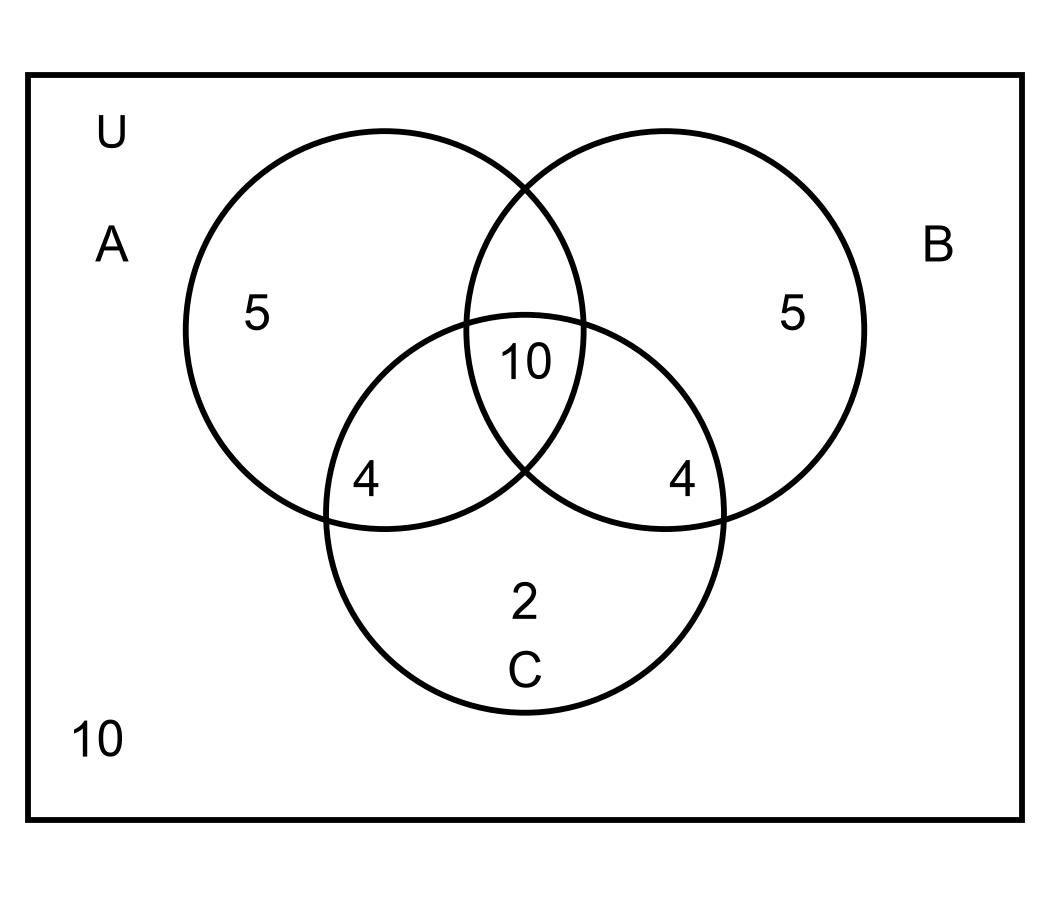
\includegraphics[width=0.38\textwidth]{figures/venn_50_ABC.png}
\end{center}
\step{所以单选物理、化学的人数至多 10 人.}
\step{所以至多选选择物理和化学这两门课程的学生人数至多 $10+10=20$ 人.}
\step{故选 C.}
\solend

\fi

\item 设 $k\geqslant 1,\,k\in\mathbb{N}$，已知集合 $M=\{1,2,3,4,5\}$，若集合 $N_1,N_2,\dots,N_k$ 是集合 $M$ 的 $k$ 个不同非空子集，且 $N_1\cup N_2\cup\dots\cup N_k\neq M$，则 $k$ 的最大值为\mbox{（\quad）.}

\keepwithprev
A. $15$\qquad B. $16$\qquad C. $31$\qquad D. $32$

\ans{A}

\ifanswer
\solbegin
\step{由 $N_1\cup N_2\cup\dots\cup N_k\neq M$ 得所有非空子集的并集缺少集合 $M$ 中至少一个元素.}
\step{假设缺少元素 1，则所有非空子集 $N_i$ 均不含元素 1，即 $N_i$ 是集合 $\{2,3,4,5\}$ 非空子集，集合 $\{2,3,4,5\}$ 的非空子集个数为 $2^4-1=15$，且这些子集 $N_i$ 的并集必不含 1，满足条件.}
\step{假设 $k\geqslant 16$，要满足所有非空子集的并集不等于集合 $M$，必须至少有一个集合 $M$ 中的元素不在任何一个子集中，否则并集就会等于 $M$.}
\step{设这个缺失的元素是 1，那么 $k$ 个非空集都不含元素 1，即每个子集都是集合 $\{2,3,4,5\}$ 的非空子集.}
\step{而集合 $\{2,3,4,5\}$ 只有 $2^4-1=15$ 个不同的非空子集，所以无法从中取出至少 16 个不同的非空子集.}
\step{因此假设不成立，$k$ 必须小于 16.}
\step{所以 $k$ 的最大值为 15，故选 A.}
\solend

\fi

% 注：原卷此题的差集记号是反斜杠 $A\setminus B$（本稿曾误作 $A\vee B$）；$C$ 的集合描述里原卷留了一条
%     待填横线“$x\in A\underline{\quad}B$”（选项按填入的符号分四种情形），本稿曾误作 $\vee\vee$。
%     2026-09-15 回原图核对时已按原卷改回。
\item 对于集合 $A$、$B$，定义 $A\setminus B=\{x\mid x\in A\text{ 且 }x\notin B\}$，则对于集合 $A=\{x\mid x=6n+5,\,n\in\mathbb{N}\}$，$B=\{y\mid y=3m+7,\,m\in\mathbb{N}\}$，$C=\{x\mid x\in A\underline{\hspace{4em}}B\text{ 且 }x<1000\}$，以下说法正确的是\mbox{（\quad）.}

\keepwithprev
A. 若在横线上填入“$\cap$”，则 $C$ 的真子集有 $2^{12}-1$ 个；

B. 若在横线上填入“$\cup$”，则 $C$ 中元素个数大于 250；

C. 若在横线上填入“$\setminus$”，则 $C$ 的非空真子集有 $2^{153}-2$ 个；

% 注：原卷选项 D 作“若在横线上填入“$\cup\complement_{\mathbb N}$”，则 $\complement_{\mathbb N}C$ 中元素个数为 13”；
%     本稿曾把 $\complement_{\mathbb N}$ 抄成 $\varnothing$、把 $\complement_{\mathbb N}C$ 抄成 $C\setminus C$，2026-09-15 回原图核对时已订正。
D. 若在横线上填入“$\cup\complement_{\mathbb{N}}$”，则 $\complement_{\mathbb{N}}C$ 中元素个数为 13.

\ans{B}

\ifanswer
\solbegin
\step{$x=6n+5=3(2n+1)+2$，$y=3m+7=3(m+2)+1$，集合 $A$、$B$ 无公共元素.}
\step{选项 A 中，集合 $C$ 为空集，没有真子集，$A$ 错；}
\step{选项 B 中，由 $6n+5<1000$ 得 $n<165\tfrac{5}{6}$，由 $3m+7<1000$ 得 $m<331$，因此 $C$ 中元素个数为 $166+331=497$，B 正确；}
\step{选项 C 中，$C$ 中元素个数为 166，非空真子集个数为 $2^{166}-2$，C 错；}
% 注：原卷此行作“$\complement_{\mathbb N}C=\complement_{\mathbb N}(A\cup\complement_{\mathbb N}B)
%     =\complement_{\mathbb N}A\cap\complement_{\mathbb N}(\complement_{\mathbb N}B)=\complement_{\mathbb N}A\cap B$，
%     而 $B\subseteq\complement_{\mathbb N}A$”；本稿曾把 $\complement_{\mathbb N}$ 抄成 $C\setminus$，同日已订正。
\step{选项 D 中，$\complement_{\mathbb{N}}C=\complement_{\mathbb{N}}(A\cup\complement_{\mathbb{N}}B)=\complement_{\mathbb{N}}A\cap\complement_{\mathbb{N}}(\complement_{\mathbb{N}}B)=\complement_{\mathbb{N}}A\cap B$，而 $B\subseteq\complement_{\mathbb{N}}A$.}
\step{因此其中元素个数为 331 个，D 错.}
\step{故选 B.}
\solend

\fi
\end{enumerate}

\bigsec{三、解答题}

\begin{enumerate}
\setcounter{enumi}{16}

\item 已知集合 $A=\{x\mid x<-1\text{ 或 }x>4\}$，$B=\{x\mid m+1\leqslant x\leqslant 2m+4\}$.
\begin{enumerate}[label=(\arabic*)]
\item 若 $m=2$，求 $A\cup B$ 和 $\left(\complement_{\R} A\right)\cap B$；
\item 若 $A\cap B=\varnothing$，求 $m$ 的取值范围.
\end{enumerate}

\ans{（1）$A\cup B=\{x\mid x<-1\text{ 或 }x\geqslant 3\}$，$\left(\complement_{\R} A\right)\cap B=\{x\mid 3\leqslant x\leqslant 4\}$；（2）$(-\infty,-3)\cup[-2,0]$}

\ifanswer
\solbegin
\stepm{(1)}{当 $m=2$ 时，集合 $B=\{x\mid 3\leqslant x\leqslant 8\}$.}
\step{又因为 $A=\{x\mid x<-1\text{ 或 }x>4\}$，则 $\complement_{\R}A=\{x\mid -1\leqslant x\leqslant 4\}$，所以 $A\cup B=\{x\mid x<-1\text{ 或 }x\geqslant 3\}$，$\left(\complement_{\R} A\right)\cap B=\{x\mid 3\leqslant x\leqslant 4\}$.}
\stepm{(2)}{因为 $A\cap B=\varnothing$，所以当 $B=\varnothing$ 时，$m+1>2m+4$，解得 $m<-3$ 满足题意；}
\step{当 $B\neq\varnothing$ 时，要满足题意，只需 $\begin{cases}m+1\leqslant 2m+4 \\ m+1\geqslant -1 \\ 2m+4\leqslant 4\end{cases}$，解得 $-2\leqslant m\leqslant 0$.}
\step{综上，实数 $m$ 的范围为 $m<-3$ 或 $-2\leqslant m\leqslant 0$，即 $(-\infty,-3)\cup[-2,0]$.}
\solend

\fi
\ansspace[6]
\item 设集合 $A=\{x\mid x^2+4x=0\}$，$B=\{x\mid x^2+2(a+1)x+a^2-1=0\}$.
\begin{enumerate}[label=(\arabic*)]
\item 写出集合 $A$ 的所有子集；
\item 若 $A\cap B=B$，求实数 $a$ 的取值范围.
\end{enumerate}

\ans{（1）$\{\varnothing,\{0\},\{-4\},\{0,-4\}\}$；（2）$a=1$ 或 $a\leqslant -1$}

\ifanswer
\solbegin
% 注：原卷此行印作“集合 $A$ 的所有子集为 $\varnothing,\{0\},\{-4\},\{0-4\}$”（末项漏逗号、且未加外层花括号）；
%     本稿按规范的列举写法给出，2026-09-15 回原图核对时加注。
\stepm{(1)}{由题意得 $A=\{0,-4\}$，集合 $A$ 的所有子集为 $\varnothing,\{0\},\{-4\},\{0,-4\}$.}
\stepm{(2)}{由 $A\cap B=B$ 得 $B\subseteq A$，所以 $B=\{0\}$ 或 $B=\{-4\}$ 或 $B=\{0,-4\}$ 或 $B=\varnothing$.}
\step{若 $B=\{0\}$ 时，$x^2+2(a+1)x+a^2-1=0$ 有两个相等的根 $0$，则 $\begin{cases}-2(a+1)=0 \\ a^2-1=-4\times(-4)\end{cases}$，解得 $a=-1$.}
\step{若 $B=\{-4\}$ 时，$x^2+2(a+1)x+a^2-1=0$ 有两个相等的根 $-4$，则 $\left\{\begin{matrix}-2(a+1)=-8 \\ a^2-1=-4\times(-4)\end{matrix}\right.$，$a$ 无解.}
\step{若 $B=\{0,-4\}$ 时，$x^2+2(a+1)x+a^2-1=0$ 有两个不相等的根 $0$ 和 $-4$，则 $\begin{cases}-2(a+1)=-4 \\ a^2-1=0\end{cases}$，解得 $a=1$.}
\step{当 $B=\varnothing$ 时，$x^2+2(a+1)x+a^2-1=0$ 无实数根，$\Delta=[2(a+1)]^2-4(a^2-1)=8a+8<0$，得 $a<-1$.}
\step{综上，$a=1$ 或 $a\leqslant -1$.}
\solend

\fi
\ansspace[6]
\item 已知集合 $A=\{x\mid x^2-5x+6=0\}$，$B=\{x\mid mx+1=0\}$，$C=\{x\in\mathbb{N}\mid \sqrt{x}\leqslant 1\}$，且 $A\cup B=A$.
\begin{enumerate}[label=(\arabic*)]
\item 求集合 $M=\{x\mid x\subseteq A\}$ 的真子集的个数；
\item 求实数 $m$ 的值组成的集合；
% 注：原卷本题的定义作“集合 $E=\{x\mid -x\in D,\,2-x^2\notin D\}$”；本稿曾把 $\notin$ 抄成 $\in$
%     （那样 $E=\varnothing$，与答案 $-5$ 冲突），2026-09-15 回原图核对时已订正。
\item 若集合 $D=A\cup C$，定义：集合 $E=\{x\mid -x\in D,\,2-x^2\notin D\}$，求集合 $E$ 中所有元素的和.
\end{enumerate}

\ans{（1）$15$；（2）$\left\{0,-\tfrac{1}{2},-\tfrac{1}{3}\right\}$；（3）$-5$}

\ifanswer
\solbegin
\stepm{(1)}{$A=\{x\mid x^2-5x+6=0\}=\{2,3\}$.}
\step{由 $M=\{x\mid x\subseteq A\}$ 得 $M$ 是 $A$ 的所有子集构成的集合，集合 $A$ 有 2 个元素，故 $A$ 的子集共 $2^2=4$ 个，即 $M$ 含 4 个元素，$M$ 的真子集个数为 $2^4-1=15$.}
\stepm{(2)}{由 (1) 得 $A=\{2,3\}$，集合 $B=\{x\mid mx+1=0\}$.}
\step{由 $A\cup B=A$ 得 $B\subseteq A$，分两种情况：① 当 $m=0$ 时，方程 $mx+1=0$ 无解，$B=\varnothing$，空集是任意集合的子集，符合条件；}
\stepm{②}{当 $m\neq 0$ 时，$B=\{-\tfrac{1}{m}\}$，由 $B\subseteq A$ 得 $-\tfrac{1}{m}=2$ 或 $-\tfrac{1}{m}=3$，解得 $m=-\tfrac{1}{2}$ 或 $m=-\tfrac{1}{3}$.}
\step{实数 $m$ 的取值集合为 $\left\{0,-\tfrac{1}{2},-\tfrac{1}{3}\right\}$.}
\stepm{(3)}{由 (1) 得 $A=\{2,3\}$.}
\step{由 $x\in\mathbb{N}$ 且 $\sqrt{x}\leqslant 1$，得 $x=0$ 或 $x=1$，故 $C=\{0,1\}$.}
\step{所以 $D=A\cup C=\{0,1,2,3\}$.}
\step{由 $-x\in D$ 得 $x$ 的候选值为 $0,-1,-2,-3$.}
\step{由于集合 $E=\{x\mid -x\in D,\,2-x^2\in D\}$，当 $x=0$ 时，$2-x^2=2\in D$，不符合题意；}
\step{当 $x=-1$ 时，$2-x^2=1\in D$，不符合题意；}
\step{当 $x=-2$ 时，$2-x^2=-2\notin D$，符合题意；}
\step{当 $x=-3$ 时，$2-x^2=-7\notin D$，符合题意.}
\step{故 $E=\{-2,-3\}$，所有元素的和为 $-2+(-3)=-5$.}
\solend

\fi
\ansspace[8]
\item 设集合 $M$ 是至少含有两个元素的数集，若 $M$ 中存在两个元素 $x$、$y$ 满足它们的积 $xy\in M$，则称 $M$ 为可积数集.
\begin{enumerate}[label=(\arabic*)]
\item 设集合 $A=\{2,3,5\}$，试判断 $A$ 是否为可积数集？并说明理由；
\item 设集合 $B=\{2,3,4,a\}$，若 $B$ 为可积数集，求实数 $a$ 的取值集合；
\item 设集合 $D=\{x\mid t<x<t+2\}$，若 $D$ 不是可积数集，求实数 $t$ 的取值范围.
\end{enumerate}

% 注：原卷本题【答案】与文末解析的结论都含 $\frac{3}{4}$；本稿曾漏掉 $\frac{3}{4}$
%     （与本稿自己的解析结论不一致），2026-09-15 回原图核对时已订正。
\ans{（1）否；（2）$\left\{0,\tfrac{1}{2},\tfrac{2}{3},\tfrac{3}{4},1,\tfrac{4}{3},\tfrac{3}{2},6,8,12\right\}$；（3）$t\in(-\infty,-2]\cup[2,+\infty)$}

\ifanswer
\solbegin
\stepm{(1)}{因为 $2\times 3=6\notin A$，$2\times 5=10\notin A$，$3\times 5=15\notin A$，所以 $A$ 中任意两个元素的积都不是 $A$ 中的元素，即 $A$ 不是可积数集.}
\stepm{(2)}{若 $B=\{2,3,4,a\}$ 为可积数集，则 $2\times 3=6\in B$，或 $2\times 4=8\in B$ 或 $3\times 4=12\in B$ 或 $2a\in B$ 或 $3a\in B$ 或 $4a\in B$.}
\step{若 $6\in B$，则 $a=6$；}
\step{若 $8\in B$，则 $a=8$；}
\step{若 $12\in B$，则 $a=12$；}
\step{若 $2a\in B$，则 $2a=2$ 或 $2a=3$ 或 $2a=4$ 或 $2a=a$，解得 $a=1$ 或 $a=\tfrac{3}{2}$ 或 $a=2$（舍）或 $a=0$；}
\step{若 $3a\in B$，则 $3a=2$ 或 $3a=3$ 或 $3a=4$ 或 $3a=a$，解得 $a=\tfrac{2}{3}$ 或 $a=1$ 或 $a=\tfrac{4}{3}$ 或 $a=0$；}
\step{若 $4a\in B$，则 $4a=2$ 或 $4a=3$ 或 $4a=4$ 或 $4a=a$，解得 $a=\tfrac{1}{2}$ 或 $a=\tfrac{3}{4}$ 或 $a=1$ 或 $a=0$.}
\step{综上，实数 $a$ 的取值集合为 $\left\{0,\tfrac{1}{2},\tfrac{2}{3},\tfrac{3}{4},1,\tfrac{4}{3},\tfrac{3}{2},6,8,12\right\}$.}
\stepm{(3)}{若 $D=\{x\mid t<x<t+2\}$ 不是可积数集，则 $\forall x,y\in(t,t+2)$，$xy\notin(t,t+2)$.}
\step{当 $t+2\leqslant 0$，即 $t\leqslant -2$ 时，$0\leqslant(t+2)^2<xy<t^2$，此时 $xy\notin D$，满足题意；}
\step{当 $t\geqslant 0$ 时，$0\leqslant t^2<xy<(t+2)^2$，因为 $(t+2)^2>t$，所以若 $xy\notin D$，则 $t^2\geqslant t+2$，即 $t^2-t-2\geqslant 0$，解得 $t\geqslant 2$ 或 $t\leqslant -1$，此时 $t\geqslant 2$ 满足题意；}
% 注：原卷此句作“当 $t<0<t+2$，即 $-2<t<0$ 时，$\exists x=0$，$xy=0\in D$，不满足题意，舍去”；
%     本稿曾把 $\in D$ 抄成 $\notin D$（$-2<t<0$ 时 $0\in(t,t+2)$，确有 $0\in D$），同日已订正。
\step{当 $t<0<t+2$，即 $-2<t<0$ 时，$\exists x=0$，$xy=0\in D$，不满足题意，舍去.}
\step{综上，所求实数 $t$ 的取值范围为 $t\geqslant 2$ 或 $t\leqslant -2$，故 $t\in(-\infty,-2]\cup[2,+\infty)$.}
\solend

\fi
\ansspace[8]
\ansneed{7cm}
\item 已知集合 $A$ 为非空数集，定义：$S=\{x\mid x=a+b,\,a,b\in A\}$，$T=\{x\mid x=|a-b|,a,b\in A\}$（实数 $a$、$b$ 可以相同）.
\begin{enumerate}[label=(\arabic*)]
\item 若集合 $A=\{2,5\}$，直接写出集合 $S$、$T$；
\item 若集合 $A=\{x_1,x_2,x_3,x_4\}$，$x_1<x_2<x_3<x_4$，且 $T=A$，求证：$x_1+x_4=x_3+x_2$；
\item 若集合 $A\subseteq\{x\mid 0\leqslant x\leqslant 2025,\,x\in\mathbb{N}\}$，$S\cap T=\varnothing$，记 $|A|$ 为集合 $A$ 中的元素个数，求 $|A|$ 的最大值.
\end{enumerate}

\ans{（1）$S=\{4,7,10\}$，$T=\{0,3\}$；（2）略；（3）$1350$}

\ifanswer
\solbegin
\stepm{(1)}{$S=\{4,7,10\}$，$T=\{0,3\}$.}
\stepm{(2)}{由集合 $A=\{x_1,x_2,x_3,x_4\}$，$x_1<x_2<x_3<x_4$，则 $T$ 集合的元素在 $0,x_2-x_1,x_3-x_1,x_4-x_1,x_3-x_2,x_4-x_2,x_4-x_3$ 中，且 $0<x_2-x_1<x_3-x_1<x_4-x_1$，$x_3-x_2<x_4-x_2<x_4-x_3$，因为 $A=T$，所以 $A$ 中最大元素 $x_4$ 必在 $T$ 中，而 $x_4-x_1$ 为 7 个元素中的最大者.}
\step{故 $x_4=x_4-x_1$，即 $x_1=0$.}
\step{故 $A=\{0,x_2,x_3,x_4\}$.}
\step{则 $x_3-x_2$、$x_4-x_2$、$x_4-x_3$ 与 $x_2$、$x_3$、$x_4$ 重复.}
\step{而 $0<x_3-x_2<x_3$，故 $x_3-x_2=x_2$，即 $x_3=2x_2$.}
% 注：原卷此句作“而 $0<x_4-x_3<x_4$，故 $x_4-x_3=x_2$ 或 $x_4-x_3=x_3$”；本稿曾把上界写成 $x_3$
%     （那样排除不了 $x_4-x_3=x_3$，与后半句自相矛盾），2026-09-15 回原图核对时已订正。
\step{而 $0<x_4-x_3<x_4$，故 $x_4-x_3=x_2$ 或 $x_4-x_3=x_3$.}
\step{若 $x_4=2x_3=4x_2$，则 $A=\{0,x_2,2x_2,4x_2\}$，$4x_2-x_2=3x_2\notin T$，与题设矛盾.}
\step{故 $x_4-x_3=x_2$，又因为 $x_1=0$，所以 $x_4+x_1=x_3+x_2$.}
% 注：原卷此行作“则 $2a_1<a_1+a_2<a_1+a_3<\cdots<a_1+a_k<a_2+a_k<a_3+a_k<\cdots<a_{k-1}+a_k<2a_k$，
%     所以 $|S|\geqslant 2k-1$，$a_1-a_1<a_2-a_1<a_3-a_1<\cdots<a_k-a_1$，所以 $|T|\geqslant k$”；
%     本稿曾把这个不等式链抄乱（作 $\cdots<a_1+a_k<a_2+a_3<a_k+a_k\leqslant 2a_k$）且把首项写成 $a_i-a_1$，
%     2026-09-15 回原图核对时已订正。
\stepm{(3)}{设 $A=\{a_1,a_2,\dots,a_k\}$ 满足题意，其中 $a_1<a_2<\dots<a_k$，则 $2a_1<a_1+a_2<a_1+a_3<\dots<a_1+a_k<a_2+a_k<a_3+a_k<\dots<a_{k-1}+a_k<2a_k$，所以 $|S|\geqslant 2k-1$，$a_1-a_1<a_2-a_1<a_3-a_1<\dots<a_k-a_1$，所以 $|T|\geqslant k$.}
\step{因为 $S\cap T=\varnothing$，由容斥原理得 $|S\cup T|=|S|+|T|\geqslant 3k-1$.}
\step{$S\cup T$ 中最小的元素为 0，最大的元素为 $2a_k$，$|S\cup T|\leqslant 2a_k+1$，所以 $3k-1\leqslant 2a_k+1\leqslant 2\times 2025+1\,(k\geqslant 1,k\in\mathbb{N})$，即 $3k-1\leqslant 4051$，解得 $k\leqslant 1350\tfrac{2}{3}$.}
\step{实际上 $A=\{676,677,678,\dots,2025\}$ 时满足题意，证明如下：设 $A=\{m,m+1,m+2,\dots,2025\}$，$m\in\mathbb{N}$.}
\step{则 $S=\{2m,2m+1,2m+2,\dots,4050\}$，$T=\{0,1,2,\dots,2025-m\}$.}
\step{由题意得 $2025-m<2m$，即 $m>675$.}
\step{所以 $A=\{676,677,678,\dots,2025\}$ 时满足题意，此时集合 $A$ 中的元素的个数最多.}
\step{综上所述，集合 $A$ 中元素的个数的最大值是 1350.}
\solend

\fi
\ansspace*[10]
\end{enumerate}

\end{document}"
% 紧凑版：xelatex "\def\iscompact{1}% 高一07_交附闵行_周练1.tex —— 高一上数学“2026-2027 年交附闵行高一上周练 1”（试卷版/答案版）
% 试卷版：xelatex 高一07_交附闵行_周练1.tex
% 答案版：xelatex "\def\isanswer{1}\input{高一07_交附闵行_周练1.tex}"
% 紧凑版：xelatex "\def\iscompact{1}\input{高一07_交附闵行_周练1.tex}"
%
% 原始材料是微信公众号图文（“魔都数学加油站”，作者署名“破晓”），正文为 11 张 PNG 页
% （1080×1527）；卷面上的粉色斜水印“魔都数学加油站”属水印，未录入。原文本身就是一份
% **讲评版**——题下直接印出【答案】或【解析】，本稿把这些答案与解析移到答案版，试卷版即
% 一张干净的空卷。
%
% 与原卷的排版差异（均已在 README“说明”中交代）：
%   ① 原文自**第 3 题**起（第 1、2 题未在该文发布），源码里以 \setcounter{enumi}{2} 起编；
%   ② 原卷本就印有分节标题“一、填空题”“二、选择题”“三、解答题”（已在原图上逐页放大
%      核对过），本稿照原卷分节，只把标题改排成全稿统一的“大节标题”样式；
%   ③ 原卷的实数集、整数集符号作正体 $R$（第 7 题）、$Z$（第 11 题），本稿按全稿惯例统一
%      写作 $\R$、$\Z$；
%   ④ 第 14 题【解析】里的 Venn 图取自原卷截图（`figures/venn_50_ABC.png`，4× LANCZOS
%      放大），未用 TikZ 重绘.

\documentclass[a4paper,11pt]{article}
\usepackage{common}

\begin{document}

\examtitlest{2026--2027 学年度交附闵行高一上周练 1}{集合与常用逻辑用语}

\bigsec{一、填空题}

\begin{enumerate}
\setcounter{enumi}{2}

\item 已知集合 $A=\{2,14,x^2+5\}$，$B=\{2,2x\}$，若 $A\cap B=B$，则实数 $x=$ \blankline[2em].

\ans{$7$}

\ifanswer
\solbegin
\step{因为 $A\cap B=B$，所以 $B\subseteq A$，所以 $2x=14$ 或 $x^2+5=2x$.}
\step{$2x=14$ 时，$x=7$，此时 $A=\{2,14,54\}$，$B=\{2,14\}$ 满足题意；}
\step{$x^2+5=2x$ 时，$(x-1)^2+4=0$，无解.}
\step{所以 $x=7$.}
\solend

\fi
\item 设集合 $A=\{y\mid y=x^2-1\}$，$B=\{(x,y)\mid y=x\}$，则 $A\cap B=$ \blankline[2em].

\ans{$\varnothing$}

\item 若集合 $\{0,-1,2a\}=\{a-1,-|a|,a+1\}$，实数 $a$ 的值为 \blankline[2em].

\ans{$\pm 1$}

\ifanswer
\solbegin
\step{令 $A=\{0,-1,2a\}$，$B=\{a-1,-|a|,a+1\}$，因为 $\{0,-1,2a\}=\{a-1,-|a|,a+1\}$，若 $a-1=0$，则 $a=1$，则 $A=\{0,-1,2\}$，$B=\{0,-1,2\}$，满足要求；}
\step{若 $-|a|=0$，则 $a=0$，则 $A=\{0,-1,0\}$，不满足集合元素的互异性；}
\step{若 $a+1=0$，则 $a=-1$，则 $A=\{0,-1,-2\}$，$B=\{0,-1,-2\}$，满足要求.}
\step{故实数 $a$ 的值为 $\pm 1$.}
\solend

\fi
\item 已知全集 $U=(-4,3]$，$A=\{x\in U\mid x^2+2x-8=0\}$，$B=\{x\in U\mid -3<1-2x\leqslant 5\}$，则 $\left(\complement_U B\right)\cap A=$ \blankline[2em].

\ans{$\{2\}$}

\item 已知集合 $A=\{x\mid 1-a\leqslant x\leqslant 1+a,\,a\in\R\}$ 中只有一个整数元素，则实数 $a$ 的取值范围为 \blankline[2em].

\ans{$[0,1)$}

\ifanswer
\solbegin
\step{集合 $A=\{x\mid 1-a\leqslant x\leqslant 1+a,\,a\in\R\}$ 中只有一个整数元素，则 $A\neq\varnothing,\,1-a\leqslant 1+a$，即 $a\geqslant 0$，此时 $1\in A$，故 $\begin{cases}1+a<2 \\ 1-a>0\end{cases}$，解得 $a<1$.}
\step{故 $a\in[0,1)$.}
\solend

\fi
\item 已知全集 $U=\{x\in\mathbb{N}\mid x\leqslant 9\}$，$A\cap B=\{3\}$，$\overline{A}\cap B=\{4,6,8\}$，$A\cap\overline{B}=\{1,5\}$，则 $\overline{A}=$ \blankline[2em].

\ans{$\{0,2,4,6,7,8,9\}$}

\ifanswer
\solbegin
\step{由题意得 $U=\{x\in\mathbb{N}\mid x\leqslant 9\}=\{0,1,2,3,4,5,6,7,8,9\}$，$A\cap B=\{3\}$ 得 $A$、$B$ 中含有元素 $3$；}
\step{$\overline{A}\cap B=\{4,6,8\}$ 得 $B$ 中含有 $4$、$6$、$8$，集合 $A$ 中不含 $4$、$6$、$8$；}
\step{$A\cap\overline{B}=\{1,5\}$ 得 $A$ 含有 $1$、$5$，集合 $B$ 不含 $1$、$5$.}
\step{对于 $0$，假设集合 $A$ 中含有 $0$，由 $A\cap B=\{3\}$ 得 $B$ 不含 $0$，则 $A\cap\overline{B}$ 必含元素 $0$，与 $A\cap\overline{B}=\{1,5\}$ 矛盾.}
\step{同理可得集合 $A$ 中不含元素 $2$、$7$、$9$.}
\step{综上所述，$A=\{1,3,5\}$.}
\step{故 $\overline{A}=\{0,2,4,6,7,8,9\}$.}
\solend

\fi
\item 已知一个有四个数字元素的集合 $S$，$S$ 的所有子集的元素和（空集的元素和认为是 0）的总和为 16208，则 $S$ 的元素之和等于 \blankline[2em].

\ans{$2026$}

\ifanswer
\solbegin
\step{设 $S=\{a_1,a_2,a_3,a_4\}$，$S$ 的每个元素在所有子集中均出现 $2^3$ 次，故 $(a_1+a_2+a_3+a_4)\cdot 2^3=16208$，所以 $a_1+a_2+a_3+a_4=2026$，故 $S$ 的元素之和等于 2026.}
\solend

\fi
\item 已知集合 $M=\{x\in\mathbb{N}\mid 1\leqslant x\leqslant 12\}$，集合 $A_1$、$A_2$、$A_3$ 满足：① 每个集合都恰有 4 个元素；② $A_1\cup A_2\cup A_3=M$. 集合 $A_i\,(i=1,2,3)$ 中元素的最大值与最小值之和称为集合 $A_i$ 的特征数，记为 $X_i\,(i=1,2,3)$，则 $X_1+X_2+X_3$ 的最大值与最小值的积为 \blankline[2em].

\ans{$1485$}

\ifanswer
\solbegin
\step{集合 $M=\{x\in\mathbb{N}\mid 1\leqslant x\leqslant 12\}$ 中最小值为 1，最大值为 12.}
% 注：原卷此处印作“则 $A_1=13$”（原卷笔误，按上下文应为 $X_1=13$），本稿按 $X_1$ 规范，2026-09-15 回原图核对时加注。
\stepm{①}{若使 $X_1+X_2+X_3$ 取得最大值，不妨设 $A_1=\{1,2,3,12\}$，则 $X_1=13$，则剩余的数中最小值是 4，最大值是 11，令 $A_2=\{4,5,6,11\}$，则 $X_2=15$，则 $A_3=\{7,8,9,10\}$，$X_3=17$，则 $X_1+X_2+X_3$ 的最大值为 $13+15+17=45$；}
\stepm{②}{若使 $X_1+X_2+X_3$ 取得最小值，则 $A_1=\{1,4,5,6\}$，则 $X_1=7$，令 $A_2=\{2,7,8,9\}$，则 $X_2=11$，则 $A_3=\{3,10,11,12\}$，$X_3=15$，则此时 $X_1+X_2+X_3$ 的最小值为 $7+11+15=33$.}
\step{故 $X_1+X_2+X_3$ 的最大值与最小值的积为 $45\times 33=1485$.}
\solend

\fi
\item 对于集合 $M=\{a\mid a=x^2-y^2,\,x\in\Z,\,y\in\Z\}$，给出如下三个结论：

① 如果 $P=\{b\mid b=2n+1,\,n\in\Z\}$，那么 $P\subseteq M$；

% 注：原卷此条作“如果 $c=4n+2$，$n\in\Z$，那么 $c\notin M$”；本稿曾把 $\notin$ 抄成 $\in$
%     （那样②为假，与本卷答案 ①②③ 冲突），2026-09-15 回原图核对时已订正。
② 如果 $c=4n+2$，$n\in\Z$，那么 $c\notin M$；

③ 如果 $a_1\in M$，$a_2\in M$，那么 $a_1a_2\in M$. 其中正确结论的序号是 \blankline[2em].

\ans{①②③}

\ifanswer
\solbegin
\stepm{①}{由已知 $b=2n+1,\,n\in\Z$，则恒有 $2n+1=(n+1)^2-n^2,\,n\in\Z$，所以 $2n+1\in M$，所以 $P\subseteq M$，所以①正确；}
\stepm{②}{元素 $c=4n+2,\,n\in\Z$，若 $4n+2\in M$，则存在 $x$、$y\in\Z$ 使得 $x^2-y^2=4n+2$，所以 $4n+2=(x+y)(x-y)$，则 $x+y$ 与 $x-y$ 同奇或同偶.}
\step{若 $x+y$ 与 $x-y$ 都是奇数，则 $(x+y)(x-y)$ 为奇数，而 $4n+2$ 是偶数；}
\step{若 $x+y$ 和 $x-y$ 都是偶数，则 $(x+y)(x-y)$ 能被 4 整除，而 $4n+2$ 不能被 4 整除.}
\step{所以 $4n+2\notin M$，即 $c\notin M$，故②正确；}
\stepm{③}{因为 $a_1$、$a_2\in M$，则 $a_1a_2$ 还是整数，所以 $a_1a_2\in M$，故③正确.}
\step{故正确的是①②③.}
\solend

\fi
\item 用 $C(A)$ 表示非空集合 $A$ 中的元素的个数，定义 $A*B=|C(A)-C(B)|$，若 $A=\{x\mid x^2-2024x-2025=0\}$，$B=\{x\mid (2x^2+ax)(x^2+2ax+6)=0\}$，若 $A*B=1$，则 $a$ 的所有可能取值构成集合 $M$，则 $C(M)=$ \blankline[2em].

\ans{$5$}

\ifanswer
\solbegin
\step{$x^2-2024x-2025=0$ 得 $x=2025$ 或 $x=-1$，即 $C(A)=2$，因为 $A*B=|C(A)-C(B)|=1$，所以 $C(B)=3$ 或 $C(B)=1$.}
\step{方程 $(2x^2+ax)(x^2+2ax+6)=0$ 化为 $x(2x+a)(x^2+2ax+6)=0$.}
\step{当 $a=0$ 时，方程化为 $2x^3(x^2+6)=0$，解得 $x=0$，所以 $B=\{0\}$，$C(B)=1$，符合题意.}
\step{当 $a\neq 0$ 时，方程化为 $x=0$ 或 $x=-\tfrac{a}{2}$ 或 $x^2+2ax+6=0$.}
\step{因为 $0\neq -\tfrac{a}{2}$，$C(B)\neq 1$，故只有 $C(B)=3$.}
\step{故 $x^2+2ax+6=0$ 有两个相等的非零实数根，所以 $\Delta=4a^2-4\times 6=0$，解得 $a=\pm\sqrt{6}$，符合题意.}
\step{当 $x^2+2ax+6=0$ 有两个不相等实根，设 $x_1$、$x_2$，若 $x_1=-\tfrac{a}{2}$，由韦达定理得 $\begin{cases}x_1+x_2=-2a \\ x_1x_2=6\end{cases}$，% 注：原卷作“得 $x_2=-\frac{3a}{2}$”（由 $x_1+x_2=-2a$、$x_1=-\frac{a}{2}$ 得 $x_2=-\frac{3a}{2}$）；
%     本稿曾漏掉负号，2026-09-15 回原图核对时已订正。
得 $x_2=-\tfrac{3a}{2}$，$-\tfrac{a}{2}\cdot(-\tfrac{3a}{2})=\tfrac{3a^2}{4}=6$，解得 $a=\pm 2\sqrt{2}$，符合题意.}
\step{综上所述，$M=\{0,\sqrt{6},-\sqrt{6},2\sqrt{2},-2\sqrt{2}\}$，所以 $C(M)=5$.}
\solend

\fi
\end{enumerate}

\bigsec{二、选择题}

\begin{enumerate}
\setcounter{enumi}{12}

\item 已知集合 $A=\{1,2,3,4,5\}$，$B=\{x\mid \tfrac{x-1}{2}\in\Z,\,x\in A\}$，则集合 $B$ 的真子集个数为\mbox{（\quad）.}

\keepwithprev
A. $3$\qquad B. $5$\qquad C. $7$\qquad D. $15$

\ans{C}

\ifanswer
\solbegin
\step{已知集合 $A=\{1,2,3,4,5\}$，$B=\{x\mid\tfrac{x-1}{2}\in\Z,\,x\in A\}$.}
\step{因为 $\tfrac{x-1}{2}\in\Z$，所以 $x$ 为奇数，所以 $B=\{1,3,5\}$.}
\step{所以集合 $B$ 中有 3 个元素，所以集合 $B$ 的真子集个数为 $2^3-1=7$.}
\step{故选 C.}
\solend

\fi

\item 高一二班共有学生 50 人，每名学生要从物理、化学、生物、历史、地理、政治这六门课程中选择三门课程进行学习. 已知选择物理、化学、生物的学生各有至少 20 人，这三门课程都不选的有 10 人，这三门课程都选的有 10 人，在这三门课程中选择任意两门课程的都至少有 14 人，物理、化学只选一科的学生都至少 5 人，那么选择物理和化学这两门课程的学生人数至多\mbox{（\quad）.}

\keepwithprev
A. $18$\qquad B. $19$\qquad C. $20$\qquad D. $21$

\ans{C}

\ifanswer
\solbegin
\step{可以把学生 50 人看作一个集合 $U$，选择物理的人数组成集合 $A$，选择化学的人数组成集合 $B$，选择生物的人数组成集合 $C$.}
\step{要使选择物理和化学这两门课程的学生人数最多，除这三门课程都不选的有 10 人，这三门课程都选的有 10 人，则其他科选择人数均为最少，因为物理、化学只选一科的学生都至少 5 人，即得到单选物理的最少 5 人，单选化学的最少 5 人.}
\step{因为在这三门课程中选择任意两门课程的都至少有 14 人，单选化学、生物的最少 4 人，单选物理、生物的最少 4 人.}
\step{因为选择物理、化学、生物的学生各有至少 20 人，所以单选生物的最少 2 人.}
\step{以上人数最少 30 人，可作出如图所示的韦恩图：}
% 注：原卷此处印有一张韦恩图（三个圆 $A$、$B$、$C$，$A$ 独有 5、$B$ 独有 5、三集合公共 10、
%     $A\cap C$ 独有 4、$B\cap C$ 独有 4、$C$ 独有 2、三集合之外 10）；本稿此前漏排此图而正文仍作
%     “如图”，2026-09-15 回原图核对时按原卷截图补入（见 figures/venn_50_ABC.png）。
\begin{center}
% 插图取自原卷截图（裁去截图残影后 4× LANCZOS 放大），不用 TikZ 手绘
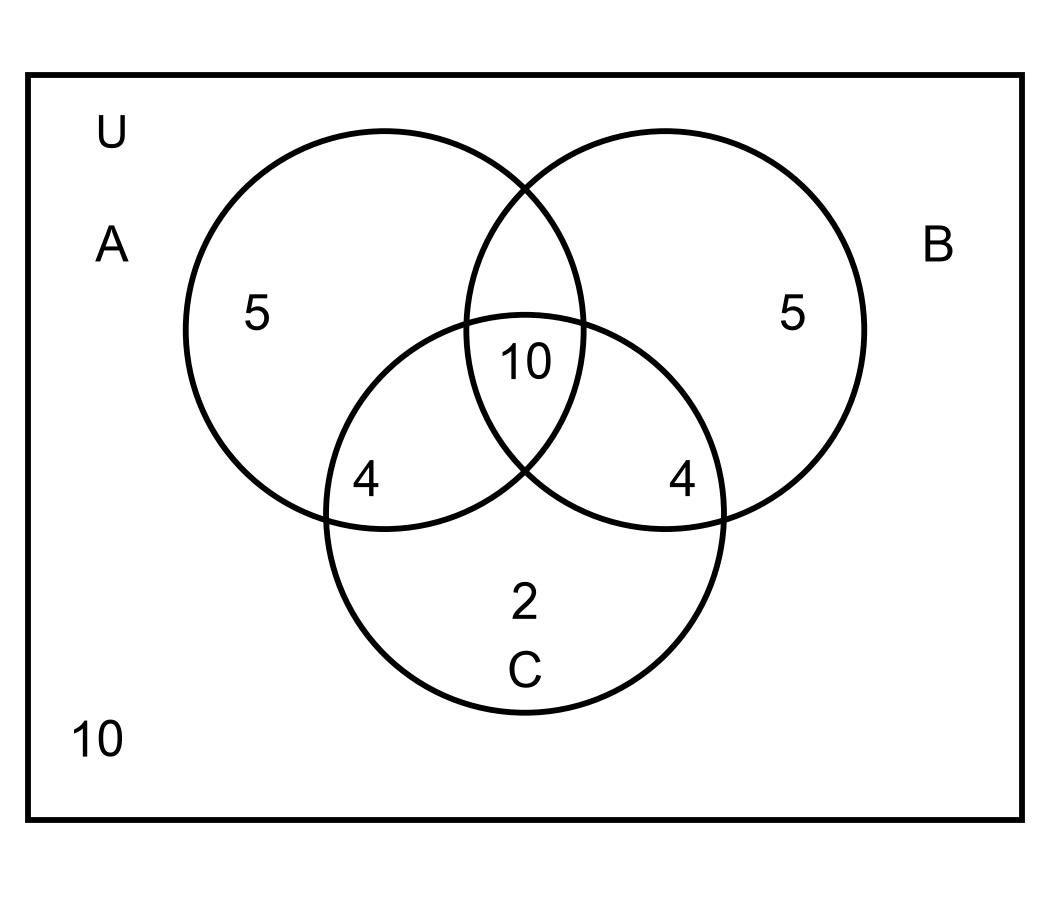
\includegraphics[width=0.38\textwidth]{figures/venn_50_ABC.png}
\end{center}
\step{所以单选物理、化学的人数至多 10 人.}
\step{所以至多选选择物理和化学这两门课程的学生人数至多 $10+10=20$ 人.}
\step{故选 C.}
\solend

\fi

\item 设 $k\geqslant 1,\,k\in\mathbb{N}$，已知集合 $M=\{1,2,3,4,5\}$，若集合 $N_1,N_2,\dots,N_k$ 是集合 $M$ 的 $k$ 个不同非空子集，且 $N_1\cup N_2\cup\dots\cup N_k\neq M$，则 $k$ 的最大值为\mbox{（\quad）.}

\keepwithprev
A. $15$\qquad B. $16$\qquad C. $31$\qquad D. $32$

\ans{A}

\ifanswer
\solbegin
\step{由 $N_1\cup N_2\cup\dots\cup N_k\neq M$ 得所有非空子集的并集缺少集合 $M$ 中至少一个元素.}
\step{假设缺少元素 1，则所有非空子集 $N_i$ 均不含元素 1，即 $N_i$ 是集合 $\{2,3,4,5\}$ 非空子集，集合 $\{2,3,4,5\}$ 的非空子集个数为 $2^4-1=15$，且这些子集 $N_i$ 的并集必不含 1，满足条件.}
\step{假设 $k\geqslant 16$，要满足所有非空子集的并集不等于集合 $M$，必须至少有一个集合 $M$ 中的元素不在任何一个子集中，否则并集就会等于 $M$.}
\step{设这个缺失的元素是 1，那么 $k$ 个非空集都不含元素 1，即每个子集都是集合 $\{2,3,4,5\}$ 的非空子集.}
\step{而集合 $\{2,3,4,5\}$ 只有 $2^4-1=15$ 个不同的非空子集，所以无法从中取出至少 16 个不同的非空子集.}
\step{因此假设不成立，$k$ 必须小于 16.}
\step{所以 $k$ 的最大值为 15，故选 A.}
\solend

\fi

% 注：原卷此题的差集记号是反斜杠 $A\setminus B$（本稿曾误作 $A\vee B$）；$C$ 的集合描述里原卷留了一条
%     待填横线“$x\in A\underline{\quad}B$”（选项按填入的符号分四种情形），本稿曾误作 $\vee\vee$。
%     2026-09-15 回原图核对时已按原卷改回。
\item 对于集合 $A$、$B$，定义 $A\setminus B=\{x\mid x\in A\text{ 且 }x\notin B\}$，则对于集合 $A=\{x\mid x=6n+5,\,n\in\mathbb{N}\}$，$B=\{y\mid y=3m+7,\,m\in\mathbb{N}\}$，$C=\{x\mid x\in A\underline{\hspace{4em}}B\text{ 且 }x<1000\}$，以下说法正确的是\mbox{（\quad）.}

\keepwithprev
A. 若在横线上填入“$\cap$”，则 $C$ 的真子集有 $2^{12}-1$ 个；

B. 若在横线上填入“$\cup$”，则 $C$ 中元素个数大于 250；

C. 若在横线上填入“$\setminus$”，则 $C$ 的非空真子集有 $2^{153}-2$ 个；

% 注：原卷选项 D 作“若在横线上填入“$\cup\complement_{\mathbb N}$”，则 $\complement_{\mathbb N}C$ 中元素个数为 13”；
%     本稿曾把 $\complement_{\mathbb N}$ 抄成 $\varnothing$、把 $\complement_{\mathbb N}C$ 抄成 $C\setminus C$，2026-09-15 回原图核对时已订正。
D. 若在横线上填入“$\cup\complement_{\mathbb{N}}$”，则 $\complement_{\mathbb{N}}C$ 中元素个数为 13.

\ans{B}

\ifanswer
\solbegin
\step{$x=6n+5=3(2n+1)+2$，$y=3m+7=3(m+2)+1$，集合 $A$、$B$ 无公共元素.}
\step{选项 A 中，集合 $C$ 为空集，没有真子集，$A$ 错；}
\step{选项 B 中，由 $6n+5<1000$ 得 $n<165\tfrac{5}{6}$，由 $3m+7<1000$ 得 $m<331$，因此 $C$ 中元素个数为 $166+331=497$，B 正确；}
\step{选项 C 中，$C$ 中元素个数为 166，非空真子集个数为 $2^{166}-2$，C 错；}
% 注：原卷此行作“$\complement_{\mathbb N}C=\complement_{\mathbb N}(A\cup\complement_{\mathbb N}B)
%     =\complement_{\mathbb N}A\cap\complement_{\mathbb N}(\complement_{\mathbb N}B)=\complement_{\mathbb N}A\cap B$，
%     而 $B\subseteq\complement_{\mathbb N}A$”；本稿曾把 $\complement_{\mathbb N}$ 抄成 $C\setminus$，同日已订正。
\step{选项 D 中，$\complement_{\mathbb{N}}C=\complement_{\mathbb{N}}(A\cup\complement_{\mathbb{N}}B)=\complement_{\mathbb{N}}A\cap\complement_{\mathbb{N}}(\complement_{\mathbb{N}}B)=\complement_{\mathbb{N}}A\cap B$，而 $B\subseteq\complement_{\mathbb{N}}A$.}
\step{因此其中元素个数为 331 个，D 错.}
\step{故选 B.}
\solend

\fi
\end{enumerate}

\bigsec{三、解答题}

\begin{enumerate}
\setcounter{enumi}{16}

\item 已知集合 $A=\{x\mid x<-1\text{ 或 }x>4\}$，$B=\{x\mid m+1\leqslant x\leqslant 2m+4\}$.
\begin{enumerate}[label=(\arabic*)]
\item 若 $m=2$，求 $A\cup B$ 和 $\left(\complement_{\R} A\right)\cap B$；
\item 若 $A\cap B=\varnothing$，求 $m$ 的取值范围.
\end{enumerate}

\ans{（1）$A\cup B=\{x\mid x<-1\text{ 或 }x\geqslant 3\}$，$\left(\complement_{\R} A\right)\cap B=\{x\mid 3\leqslant x\leqslant 4\}$；（2）$(-\infty,-3)\cup[-2,0]$}

\ifanswer
\solbegin
\stepm{(1)}{当 $m=2$ 时，集合 $B=\{x\mid 3\leqslant x\leqslant 8\}$.}
\step{又因为 $A=\{x\mid x<-1\text{ 或 }x>4\}$，则 $\complement_{\R}A=\{x\mid -1\leqslant x\leqslant 4\}$，所以 $A\cup B=\{x\mid x<-1\text{ 或 }x\geqslant 3\}$，$\left(\complement_{\R} A\right)\cap B=\{x\mid 3\leqslant x\leqslant 4\}$.}
\stepm{(2)}{因为 $A\cap B=\varnothing$，所以当 $B=\varnothing$ 时，$m+1>2m+4$，解得 $m<-3$ 满足题意；}
\step{当 $B\neq\varnothing$ 时，要满足题意，只需 $\begin{cases}m+1\leqslant 2m+4 \\ m+1\geqslant -1 \\ 2m+4\leqslant 4\end{cases}$，解得 $-2\leqslant m\leqslant 0$.}
\step{综上，实数 $m$ 的范围为 $m<-3$ 或 $-2\leqslant m\leqslant 0$，即 $(-\infty,-3)\cup[-2,0]$.}
\solend

\fi
\ansspace[6]
\item 设集合 $A=\{x\mid x^2+4x=0\}$，$B=\{x\mid x^2+2(a+1)x+a^2-1=0\}$.
\begin{enumerate}[label=(\arabic*)]
\item 写出集合 $A$ 的所有子集；
\item 若 $A\cap B=B$，求实数 $a$ 的取值范围.
\end{enumerate}

\ans{（1）$\{\varnothing,\{0\},\{-4\},\{0,-4\}\}$；（2）$a=1$ 或 $a\leqslant -1$}

\ifanswer
\solbegin
% 注：原卷此行印作“集合 $A$ 的所有子集为 $\varnothing,\{0\},\{-4\},\{0-4\}$”（末项漏逗号、且未加外层花括号）；
%     本稿按规范的列举写法给出，2026-09-15 回原图核对时加注。
\stepm{(1)}{由题意得 $A=\{0,-4\}$，集合 $A$ 的所有子集为 $\varnothing,\{0\},\{-4\},\{0,-4\}$.}
\stepm{(2)}{由 $A\cap B=B$ 得 $B\subseteq A$，所以 $B=\{0\}$ 或 $B=\{-4\}$ 或 $B=\{0,-4\}$ 或 $B=\varnothing$.}
\step{若 $B=\{0\}$ 时，$x^2+2(a+1)x+a^2-1=0$ 有两个相等的根 $0$，则 $\begin{cases}-2(a+1)=0 \\ a^2-1=-4\times(-4)\end{cases}$，解得 $a=-1$.}
\step{若 $B=\{-4\}$ 时，$x^2+2(a+1)x+a^2-1=0$ 有两个相等的根 $-4$，则 $\left\{\begin{matrix}-2(a+1)=-8 \\ a^2-1=-4\times(-4)\end{matrix}\right.$，$a$ 无解.}
\step{若 $B=\{0,-4\}$ 时，$x^2+2(a+1)x+a^2-1=0$ 有两个不相等的根 $0$ 和 $-4$，则 $\begin{cases}-2(a+1)=-4 \\ a^2-1=0\end{cases}$，解得 $a=1$.}
\step{当 $B=\varnothing$ 时，$x^2+2(a+1)x+a^2-1=0$ 无实数根，$\Delta=[2(a+1)]^2-4(a^2-1)=8a+8<0$，得 $a<-1$.}
\step{综上，$a=1$ 或 $a\leqslant -1$.}
\solend

\fi
\ansspace[6]
\item 已知集合 $A=\{x\mid x^2-5x+6=0\}$，$B=\{x\mid mx+1=0\}$，$C=\{x\in\mathbb{N}\mid \sqrt{x}\leqslant 1\}$，且 $A\cup B=A$.
\begin{enumerate}[label=(\arabic*)]
\item 求集合 $M=\{x\mid x\subseteq A\}$ 的真子集的个数；
\item 求实数 $m$ 的值组成的集合；
% 注：原卷本题的定义作“集合 $E=\{x\mid -x\in D,\,2-x^2\notin D\}$”；本稿曾把 $\notin$ 抄成 $\in$
%     （那样 $E=\varnothing$，与答案 $-5$ 冲突），2026-09-15 回原图核对时已订正。
\item 若集合 $D=A\cup C$，定义：集合 $E=\{x\mid -x\in D,\,2-x^2\notin D\}$，求集合 $E$ 中所有元素的和.
\end{enumerate}

\ans{（1）$15$；（2）$\left\{0,-\tfrac{1}{2},-\tfrac{1}{3}\right\}$；（3）$-5$}

\ifanswer
\solbegin
\stepm{(1)}{$A=\{x\mid x^2-5x+6=0\}=\{2,3\}$.}
\step{由 $M=\{x\mid x\subseteq A\}$ 得 $M$ 是 $A$ 的所有子集构成的集合，集合 $A$ 有 2 个元素，故 $A$ 的子集共 $2^2=4$ 个，即 $M$ 含 4 个元素，$M$ 的真子集个数为 $2^4-1=15$.}
\stepm{(2)}{由 (1) 得 $A=\{2,3\}$，集合 $B=\{x\mid mx+1=0\}$.}
\step{由 $A\cup B=A$ 得 $B\subseteq A$，分两种情况：① 当 $m=0$ 时，方程 $mx+1=0$ 无解，$B=\varnothing$，空集是任意集合的子集，符合条件；}
\stepm{②}{当 $m\neq 0$ 时，$B=\{-\tfrac{1}{m}\}$，由 $B\subseteq A$ 得 $-\tfrac{1}{m}=2$ 或 $-\tfrac{1}{m}=3$，解得 $m=-\tfrac{1}{2}$ 或 $m=-\tfrac{1}{3}$.}
\step{实数 $m$ 的取值集合为 $\left\{0,-\tfrac{1}{2},-\tfrac{1}{3}\right\}$.}
\stepm{(3)}{由 (1) 得 $A=\{2,3\}$.}
\step{由 $x\in\mathbb{N}$ 且 $\sqrt{x}\leqslant 1$，得 $x=0$ 或 $x=1$，故 $C=\{0,1\}$.}
\step{所以 $D=A\cup C=\{0,1,2,3\}$.}
\step{由 $-x\in D$ 得 $x$ 的候选值为 $0,-1,-2,-3$.}
\step{由于集合 $E=\{x\mid -x\in D,\,2-x^2\in D\}$，当 $x=0$ 时，$2-x^2=2\in D$，不符合题意；}
\step{当 $x=-1$ 时，$2-x^2=1\in D$，不符合题意；}
\step{当 $x=-2$ 时，$2-x^2=-2\notin D$，符合题意；}
\step{当 $x=-3$ 时，$2-x^2=-7\notin D$，符合题意.}
\step{故 $E=\{-2,-3\}$，所有元素的和为 $-2+(-3)=-5$.}
\solend

\fi
\ansspace[8]
\item 设集合 $M$ 是至少含有两个元素的数集，若 $M$ 中存在两个元素 $x$、$y$ 满足它们的积 $xy\in M$，则称 $M$ 为可积数集.
\begin{enumerate}[label=(\arabic*)]
\item 设集合 $A=\{2,3,5\}$，试判断 $A$ 是否为可积数集？并说明理由；
\item 设集合 $B=\{2,3,4,a\}$，若 $B$ 为可积数集，求实数 $a$ 的取值集合；
\item 设集合 $D=\{x\mid t<x<t+2\}$，若 $D$ 不是可积数集，求实数 $t$ 的取值范围.
\end{enumerate}

% 注：原卷本题【答案】与文末解析的结论都含 $\frac{3}{4}$；本稿曾漏掉 $\frac{3}{4}$
%     （与本稿自己的解析结论不一致），2026-09-15 回原图核对时已订正。
\ans{（1）否；（2）$\left\{0,\tfrac{1}{2},\tfrac{2}{3},\tfrac{3}{4},1,\tfrac{4}{3},\tfrac{3}{2},6,8,12\right\}$；（3）$t\in(-\infty,-2]\cup[2,+\infty)$}

\ifanswer
\solbegin
\stepm{(1)}{因为 $2\times 3=6\notin A$，$2\times 5=10\notin A$，$3\times 5=15\notin A$，所以 $A$ 中任意两个元素的积都不是 $A$ 中的元素，即 $A$ 不是可积数集.}
\stepm{(2)}{若 $B=\{2,3,4,a\}$ 为可积数集，则 $2\times 3=6\in B$，或 $2\times 4=8\in B$ 或 $3\times 4=12\in B$ 或 $2a\in B$ 或 $3a\in B$ 或 $4a\in B$.}
\step{若 $6\in B$，则 $a=6$；}
\step{若 $8\in B$，则 $a=8$；}
\step{若 $12\in B$，则 $a=12$；}
\step{若 $2a\in B$，则 $2a=2$ 或 $2a=3$ 或 $2a=4$ 或 $2a=a$，解得 $a=1$ 或 $a=\tfrac{3}{2}$ 或 $a=2$（舍）或 $a=0$；}
\step{若 $3a\in B$，则 $3a=2$ 或 $3a=3$ 或 $3a=4$ 或 $3a=a$，解得 $a=\tfrac{2}{3}$ 或 $a=1$ 或 $a=\tfrac{4}{3}$ 或 $a=0$；}
\step{若 $4a\in B$，则 $4a=2$ 或 $4a=3$ 或 $4a=4$ 或 $4a=a$，解得 $a=\tfrac{1}{2}$ 或 $a=\tfrac{3}{4}$ 或 $a=1$ 或 $a=0$.}
\step{综上，实数 $a$ 的取值集合为 $\left\{0,\tfrac{1}{2},\tfrac{2}{3},\tfrac{3}{4},1,\tfrac{4}{3},\tfrac{3}{2},6,8,12\right\}$.}
\stepm{(3)}{若 $D=\{x\mid t<x<t+2\}$ 不是可积数集，则 $\forall x,y\in(t,t+2)$，$xy\notin(t,t+2)$.}
\step{当 $t+2\leqslant 0$，即 $t\leqslant -2$ 时，$0\leqslant(t+2)^2<xy<t^2$，此时 $xy\notin D$，满足题意；}
\step{当 $t\geqslant 0$ 时，$0\leqslant t^2<xy<(t+2)^2$，因为 $(t+2)^2>t$，所以若 $xy\notin D$，则 $t^2\geqslant t+2$，即 $t^2-t-2\geqslant 0$，解得 $t\geqslant 2$ 或 $t\leqslant -1$，此时 $t\geqslant 2$ 满足题意；}
% 注：原卷此句作“当 $t<0<t+2$，即 $-2<t<0$ 时，$\exists x=0$，$xy=0\in D$，不满足题意，舍去”；
%     本稿曾把 $\in D$ 抄成 $\notin D$（$-2<t<0$ 时 $0\in(t,t+2)$，确有 $0\in D$），同日已订正。
\step{当 $t<0<t+2$，即 $-2<t<0$ 时，$\exists x=0$，$xy=0\in D$，不满足题意，舍去.}
\step{综上，所求实数 $t$ 的取值范围为 $t\geqslant 2$ 或 $t\leqslant -2$，故 $t\in(-\infty,-2]\cup[2,+\infty)$.}
\solend

\fi
\ansspace[8]
\ansneed{7cm}
\item 已知集合 $A$ 为非空数集，定义：$S=\{x\mid x=a+b,\,a,b\in A\}$，$T=\{x\mid x=|a-b|,a,b\in A\}$（实数 $a$、$b$ 可以相同）.
\begin{enumerate}[label=(\arabic*)]
\item 若集合 $A=\{2,5\}$，直接写出集合 $S$、$T$；
\item 若集合 $A=\{x_1,x_2,x_3,x_4\}$，$x_1<x_2<x_3<x_4$，且 $T=A$，求证：$x_1+x_4=x_3+x_2$；
\item 若集合 $A\subseteq\{x\mid 0\leqslant x\leqslant 2025,\,x\in\mathbb{N}\}$，$S\cap T=\varnothing$，记 $|A|$ 为集合 $A$ 中的元素个数，求 $|A|$ 的最大值.
\end{enumerate}

\ans{（1）$S=\{4,7,10\}$，$T=\{0,3\}$；（2）略；（3）$1350$}

\ifanswer
\solbegin
\stepm{(1)}{$S=\{4,7,10\}$，$T=\{0,3\}$.}
\stepm{(2)}{由集合 $A=\{x_1,x_2,x_3,x_4\}$，$x_1<x_2<x_3<x_4$，则 $T$ 集合的元素在 $0,x_2-x_1,x_3-x_1,x_4-x_1,x_3-x_2,x_4-x_2,x_4-x_3$ 中，且 $0<x_2-x_1<x_3-x_1<x_4-x_1$，$x_3-x_2<x_4-x_2<x_4-x_3$，因为 $A=T$，所以 $A$ 中最大元素 $x_4$ 必在 $T$ 中，而 $x_4-x_1$ 为 7 个元素中的最大者.}
\step{故 $x_4=x_4-x_1$，即 $x_1=0$.}
\step{故 $A=\{0,x_2,x_3,x_4\}$.}
\step{则 $x_3-x_2$、$x_4-x_2$、$x_4-x_3$ 与 $x_2$、$x_3$、$x_4$ 重复.}
\step{而 $0<x_3-x_2<x_3$，故 $x_3-x_2=x_2$，即 $x_3=2x_2$.}
% 注：原卷此句作“而 $0<x_4-x_3<x_4$，故 $x_4-x_3=x_2$ 或 $x_4-x_3=x_3$”；本稿曾把上界写成 $x_3$
%     （那样排除不了 $x_4-x_3=x_3$，与后半句自相矛盾），2026-09-15 回原图核对时已订正。
\step{而 $0<x_4-x_3<x_4$，故 $x_4-x_3=x_2$ 或 $x_4-x_3=x_3$.}
\step{若 $x_4=2x_3=4x_2$，则 $A=\{0,x_2,2x_2,4x_2\}$，$4x_2-x_2=3x_2\notin T$，与题设矛盾.}
\step{故 $x_4-x_3=x_2$，又因为 $x_1=0$，所以 $x_4+x_1=x_3+x_2$.}
% 注：原卷此行作“则 $2a_1<a_1+a_2<a_1+a_3<\cdots<a_1+a_k<a_2+a_k<a_3+a_k<\cdots<a_{k-1}+a_k<2a_k$，
%     所以 $|S|\geqslant 2k-1$，$a_1-a_1<a_2-a_1<a_3-a_1<\cdots<a_k-a_1$，所以 $|T|\geqslant k$”；
%     本稿曾把这个不等式链抄乱（作 $\cdots<a_1+a_k<a_2+a_3<a_k+a_k\leqslant 2a_k$）且把首项写成 $a_i-a_1$，
%     2026-09-15 回原图核对时已订正。
\stepm{(3)}{设 $A=\{a_1,a_2,\dots,a_k\}$ 满足题意，其中 $a_1<a_2<\dots<a_k$，则 $2a_1<a_1+a_2<a_1+a_3<\dots<a_1+a_k<a_2+a_k<a_3+a_k<\dots<a_{k-1}+a_k<2a_k$，所以 $|S|\geqslant 2k-1$，$a_1-a_1<a_2-a_1<a_3-a_1<\dots<a_k-a_1$，所以 $|T|\geqslant k$.}
\step{因为 $S\cap T=\varnothing$，由容斥原理得 $|S\cup T|=|S|+|T|\geqslant 3k-1$.}
\step{$S\cup T$ 中最小的元素为 0，最大的元素为 $2a_k$，$|S\cup T|\leqslant 2a_k+1$，所以 $3k-1\leqslant 2a_k+1\leqslant 2\times 2025+1\,(k\geqslant 1,k\in\mathbb{N})$，即 $3k-1\leqslant 4051$，解得 $k\leqslant 1350\tfrac{2}{3}$.}
\step{实际上 $A=\{676,677,678,\dots,2025\}$ 时满足题意，证明如下：设 $A=\{m,m+1,m+2,\dots,2025\}$，$m\in\mathbb{N}$.}
\step{则 $S=\{2m,2m+1,2m+2,\dots,4050\}$，$T=\{0,1,2,\dots,2025-m\}$.}
\step{由题意得 $2025-m<2m$，即 $m>675$.}
\step{所以 $A=\{676,677,678,\dots,2025\}$ 时满足题意，此时集合 $A$ 中的元素的个数最多.}
\step{综上所述，集合 $A$ 中元素的个数的最大值是 1350.}
\solend

\fi
\ansspace*[10]
\end{enumerate}

\end{document}"
%
% 原始材料是微信公众号图文（“魔都数学加油站”，作者署名“破晓”），正文为 11 张 PNG 页
% （1080×1527）；卷面上的粉色斜水印“魔都数学加油站”属水印，未录入。原文本身就是一份
% **讲评版**——题下直接印出【答案】或【解析】，本稿把这些答案与解析移到答案版，试卷版即
% 一张干净的空卷。
%
% 与原卷的排版差异（均已在 README“说明”中交代）：
%   ① 原文自**第 3 题**起（第 1、2 题未在该文发布），源码里以 \setcounter{enumi}{2} 起编；
%   ② 原卷本就印有分节标题“一、填空题”“二、选择题”“三、解答题”（已在原图上逐页放大
%      核对过），本稿照原卷分节，只把标题改排成全稿统一的“大节标题”样式；
%   ③ 原卷的实数集、整数集符号作正体 $R$（第 7 题）、$Z$（第 11 题），本稿按全稿惯例统一
%      写作 $\R$、$\Z$；
%   ④ 第 14 题【解析】里的 Venn 图取自原卷截图（`figures/venn_50_ABC.png`，4× LANCZOS
%      放大），未用 TikZ 重绘.

\documentclass[a4paper,11pt]{article}
\usepackage{common}

\begin{document}

\examtitlest{2026--2027 学年度交附闵行高一上周练 1}{集合与常用逻辑用语}

\bigsec{一、填空题}

\begin{enumerate}
\setcounter{enumi}{2}

\item 已知集合 $A=\{2,14,x^2+5\}$，$B=\{2,2x\}$，若 $A\cap B=B$，则实数 $x=$ \blankline[2em].

\ans{$7$}

\ifanswer
\solbegin
\step{因为 $A\cap B=B$，所以 $B\subseteq A$，所以 $2x=14$ 或 $x^2+5=2x$.}
\step{$2x=14$ 时，$x=7$，此时 $A=\{2,14,54\}$，$B=\{2,14\}$ 满足题意；}
\step{$x^2+5=2x$ 时，$(x-1)^2+4=0$，无解.}
\step{所以 $x=7$.}
\solend

\fi
\item 设集合 $A=\{y\mid y=x^2-1\}$，$B=\{(x,y)\mid y=x\}$，则 $A\cap B=$ \blankline[2em].

\ans{$\varnothing$}

\item 若集合 $\{0,-1,2a\}=\{a-1,-|a|,a+1\}$，实数 $a$ 的值为 \blankline[2em].

\ans{$\pm 1$}

\ifanswer
\solbegin
\step{令 $A=\{0,-1,2a\}$，$B=\{a-1,-|a|,a+1\}$，因为 $\{0,-1,2a\}=\{a-1,-|a|,a+1\}$，若 $a-1=0$，则 $a=1$，则 $A=\{0,-1,2\}$，$B=\{0,-1,2\}$，满足要求；}
\step{若 $-|a|=0$，则 $a=0$，则 $A=\{0,-1,0\}$，不满足集合元素的互异性；}
\step{若 $a+1=0$，则 $a=-1$，则 $A=\{0,-1,-2\}$，$B=\{0,-1,-2\}$，满足要求.}
\step{故实数 $a$ 的值为 $\pm 1$.}
\solend

\fi
\item 已知全集 $U=(-4,3]$，$A=\{x\in U\mid x^2+2x-8=0\}$，$B=\{x\in U\mid -3<1-2x\leqslant 5\}$，则 $\left(\complement_U B\right)\cap A=$ \blankline[2em].

\ans{$\{2\}$}

\item 已知集合 $A=\{x\mid 1-a\leqslant x\leqslant 1+a,\,a\in\R\}$ 中只有一个整数元素，则实数 $a$ 的取值范围为 \blankline[2em].

\ans{$[0,1)$}

\ifanswer
\solbegin
\step{集合 $A=\{x\mid 1-a\leqslant x\leqslant 1+a,\,a\in\R\}$ 中只有一个整数元素，则 $A\neq\varnothing,\,1-a\leqslant 1+a$，即 $a\geqslant 0$，此时 $1\in A$，故 $\begin{cases}1+a<2 \\ 1-a>0\end{cases}$，解得 $a<1$.}
\step{故 $a\in[0,1)$.}
\solend

\fi
\item 已知全集 $U=\{x\in\mathbb{N}\mid x\leqslant 9\}$，$A\cap B=\{3\}$，$\overline{A}\cap B=\{4,6,8\}$，$A\cap\overline{B}=\{1,5\}$，则 $\overline{A}=$ \blankline[2em].

\ans{$\{0,2,4,6,7,8,9\}$}

\ifanswer
\solbegin
\step{由题意得 $U=\{x\in\mathbb{N}\mid x\leqslant 9\}=\{0,1,2,3,4,5,6,7,8,9\}$，$A\cap B=\{3\}$ 得 $A$、$B$ 中含有元素 $3$；}
\step{$\overline{A}\cap B=\{4,6,8\}$ 得 $B$ 中含有 $4$、$6$、$8$，集合 $A$ 中不含 $4$、$6$、$8$；}
\step{$A\cap\overline{B}=\{1,5\}$ 得 $A$ 含有 $1$、$5$，集合 $B$ 不含 $1$、$5$.}
\step{对于 $0$，假设集合 $A$ 中含有 $0$，由 $A\cap B=\{3\}$ 得 $B$ 不含 $0$，则 $A\cap\overline{B}$ 必含元素 $0$，与 $A\cap\overline{B}=\{1,5\}$ 矛盾.}
\step{同理可得集合 $A$ 中不含元素 $2$、$7$、$9$.}
\step{综上所述，$A=\{1,3,5\}$.}
\step{故 $\overline{A}=\{0,2,4,6,7,8,9\}$.}
\solend

\fi
\item 已知一个有四个数字元素的集合 $S$，$S$ 的所有子集的元素和（空集的元素和认为是 0）的总和为 16208，则 $S$ 的元素之和等于 \blankline[2em].

\ans{$2026$}

\ifanswer
\solbegin
\step{设 $S=\{a_1,a_2,a_3,a_4\}$，$S$ 的每个元素在所有子集中均出现 $2^3$ 次，故 $(a_1+a_2+a_3+a_4)\cdot 2^3=16208$，所以 $a_1+a_2+a_3+a_4=2026$，故 $S$ 的元素之和等于 2026.}
\solend

\fi
\item 已知集合 $M=\{x\in\mathbb{N}\mid 1\leqslant x\leqslant 12\}$，集合 $A_1$、$A_2$、$A_3$ 满足：① 每个集合都恰有 4 个元素；② $A_1\cup A_2\cup A_3=M$. 集合 $A_i\,(i=1,2,3)$ 中元素的最大值与最小值之和称为集合 $A_i$ 的特征数，记为 $X_i\,(i=1,2,3)$，则 $X_1+X_2+X_3$ 的最大值与最小值的积为 \blankline[2em].

\ans{$1485$}

\ifanswer
\solbegin
\step{集合 $M=\{x\in\mathbb{N}\mid 1\leqslant x\leqslant 12\}$ 中最小值为 1，最大值为 12.}
% 注：原卷此处印作“则 $A_1=13$”（原卷笔误，按上下文应为 $X_1=13$），本稿按 $X_1$ 规范，2026-09-15 回原图核对时加注。
\stepm{①}{若使 $X_1+X_2+X_3$ 取得最大值，不妨设 $A_1=\{1,2,3,12\}$，则 $X_1=13$，则剩余的数中最小值是 4，最大值是 11，令 $A_2=\{4,5,6,11\}$，则 $X_2=15$，则 $A_3=\{7,8,9,10\}$，$X_3=17$，则 $X_1+X_2+X_3$ 的最大值为 $13+15+17=45$；}
\stepm{②}{若使 $X_1+X_2+X_3$ 取得最小值，则 $A_1=\{1,4,5,6\}$，则 $X_1=7$，令 $A_2=\{2,7,8,9\}$，则 $X_2=11$，则 $A_3=\{3,10,11,12\}$，$X_3=15$，则此时 $X_1+X_2+X_3$ 的最小值为 $7+11+15=33$.}
\step{故 $X_1+X_2+X_3$ 的最大值与最小值的积为 $45\times 33=1485$.}
\solend

\fi
\item 对于集合 $M=\{a\mid a=x^2-y^2,\,x\in\Z,\,y\in\Z\}$，给出如下三个结论：

① 如果 $P=\{b\mid b=2n+1,\,n\in\Z\}$，那么 $P\subseteq M$；

% 注：原卷此条作“如果 $c=4n+2$，$n\in\Z$，那么 $c\notin M$”；本稿曾把 $\notin$ 抄成 $\in$
%     （那样②为假，与本卷答案 ①②③ 冲突），2026-09-15 回原图核对时已订正。
② 如果 $c=4n+2$，$n\in\Z$，那么 $c\notin M$；

③ 如果 $a_1\in M$，$a_2\in M$，那么 $a_1a_2\in M$. 其中正确结论的序号是 \blankline[2em].

\ans{①②③}

\ifanswer
\solbegin
\stepm{①}{由已知 $b=2n+1,\,n\in\Z$，则恒有 $2n+1=(n+1)^2-n^2,\,n\in\Z$，所以 $2n+1\in M$，所以 $P\subseteq M$，所以①正确；}
\stepm{②}{元素 $c=4n+2,\,n\in\Z$，若 $4n+2\in M$，则存在 $x$、$y\in\Z$ 使得 $x^2-y^2=4n+2$，所以 $4n+2=(x+y)(x-y)$，则 $x+y$ 与 $x-y$ 同奇或同偶.}
\step{若 $x+y$ 与 $x-y$ 都是奇数，则 $(x+y)(x-y)$ 为奇数，而 $4n+2$ 是偶数；}
\step{若 $x+y$ 和 $x-y$ 都是偶数，则 $(x+y)(x-y)$ 能被 4 整除，而 $4n+2$ 不能被 4 整除.}
\step{所以 $4n+2\notin M$，即 $c\notin M$，故②正确；}
\stepm{③}{因为 $a_1$、$a_2\in M$，则 $a_1a_2$ 还是整数，所以 $a_1a_2\in M$，故③正确.}
\step{故正确的是①②③.}
\solend

\fi
\item 用 $C(A)$ 表示非空集合 $A$ 中的元素的个数，定义 $A*B=|C(A)-C(B)|$，若 $A=\{x\mid x^2-2024x-2025=0\}$，$B=\{x\mid (2x^2+ax)(x^2+2ax+6)=0\}$，若 $A*B=1$，则 $a$ 的所有可能取值构成集合 $M$，则 $C(M)=$ \blankline[2em].

\ans{$5$}

\ifanswer
\solbegin
\step{$x^2-2024x-2025=0$ 得 $x=2025$ 或 $x=-1$，即 $C(A)=2$，因为 $A*B=|C(A)-C(B)|=1$，所以 $C(B)=3$ 或 $C(B)=1$.}
\step{方程 $(2x^2+ax)(x^2+2ax+6)=0$ 化为 $x(2x+a)(x^2+2ax+6)=0$.}
\step{当 $a=0$ 时，方程化为 $2x^3(x^2+6)=0$，解得 $x=0$，所以 $B=\{0\}$，$C(B)=1$，符合题意.}
\step{当 $a\neq 0$ 时，方程化为 $x=0$ 或 $x=-\tfrac{a}{2}$ 或 $x^2+2ax+6=0$.}
\step{因为 $0\neq -\tfrac{a}{2}$，$C(B)\neq 1$，故只有 $C(B)=3$.}
\step{故 $x^2+2ax+6=0$ 有两个相等的非零实数根，所以 $\Delta=4a^2-4\times 6=0$，解得 $a=\pm\sqrt{6}$，符合题意.}
\step{当 $x^2+2ax+6=0$ 有两个不相等实根，设 $x_1$、$x_2$，若 $x_1=-\tfrac{a}{2}$，由韦达定理得 $\begin{cases}x_1+x_2=-2a \\ x_1x_2=6\end{cases}$，% 注：原卷作“得 $x_2=-\frac{3a}{2}$”（由 $x_1+x_2=-2a$、$x_1=-\frac{a}{2}$ 得 $x_2=-\frac{3a}{2}$）；
%     本稿曾漏掉负号，2026-09-15 回原图核对时已订正。
得 $x_2=-\tfrac{3a}{2}$，$-\tfrac{a}{2}\cdot(-\tfrac{3a}{2})=\tfrac{3a^2}{4}=6$，解得 $a=\pm 2\sqrt{2}$，符合题意.}
\step{综上所述，$M=\{0,\sqrt{6},-\sqrt{6},2\sqrt{2},-2\sqrt{2}\}$，所以 $C(M)=5$.}
\solend

\fi
\end{enumerate}

\bigsec{二、选择题}

\begin{enumerate}
\setcounter{enumi}{12}

\item 已知集合 $A=\{1,2,3,4,5\}$，$B=\{x\mid \tfrac{x-1}{2}\in\Z,\,x\in A\}$，则集合 $B$ 的真子集个数为\mbox{（\quad）.}

\keepwithprev
A. $3$\qquad B. $5$\qquad C. $7$\qquad D. $15$

\ans{C}

\ifanswer
\solbegin
\step{已知集合 $A=\{1,2,3,4,5\}$，$B=\{x\mid\tfrac{x-1}{2}\in\Z,\,x\in A\}$.}
\step{因为 $\tfrac{x-1}{2}\in\Z$，所以 $x$ 为奇数，所以 $B=\{1,3,5\}$.}
\step{所以集合 $B$ 中有 3 个元素，所以集合 $B$ 的真子集个数为 $2^3-1=7$.}
\step{故选 C.}
\solend

\fi

\item 高一二班共有学生 50 人，每名学生要从物理、化学、生物、历史、地理、政治这六门课程中选择三门课程进行学习. 已知选择物理、化学、生物的学生各有至少 20 人，这三门课程都不选的有 10 人，这三门课程都选的有 10 人，在这三门课程中选择任意两门课程的都至少有 14 人，物理、化学只选一科的学生都至少 5 人，那么选择物理和化学这两门课程的学生人数至多\mbox{（\quad）.}

\keepwithprev
A. $18$\qquad B. $19$\qquad C. $20$\qquad D. $21$

\ans{C}

\ifanswer
\solbegin
\step{可以把学生 50 人看作一个集合 $U$，选择物理的人数组成集合 $A$，选择化学的人数组成集合 $B$，选择生物的人数组成集合 $C$.}
\step{要使选择物理和化学这两门课程的学生人数最多，除这三门课程都不选的有 10 人，这三门课程都选的有 10 人，则其他科选择人数均为最少，因为物理、化学只选一科的学生都至少 5 人，即得到单选物理的最少 5 人，单选化学的最少 5 人.}
\step{因为在这三门课程中选择任意两门课程的都至少有 14 人，单选化学、生物的最少 4 人，单选物理、生物的最少 4 人.}
\step{因为选择物理、化学、生物的学生各有至少 20 人，所以单选生物的最少 2 人.}
\step{以上人数最少 30 人，可作出如图所示的韦恩图：}
% 注：原卷此处印有一张韦恩图（三个圆 $A$、$B$、$C$，$A$ 独有 5、$B$ 独有 5、三集合公共 10、
%     $A\cap C$ 独有 4、$B\cap C$ 独有 4、$C$ 独有 2、三集合之外 10）；本稿此前漏排此图而正文仍作
%     “如图”，2026-09-15 回原图核对时按原卷截图补入（见 figures/venn_50_ABC.png）。
\begin{center}
% 插图取自原卷截图（裁去截图残影后 4× LANCZOS 放大），不用 TikZ 手绘
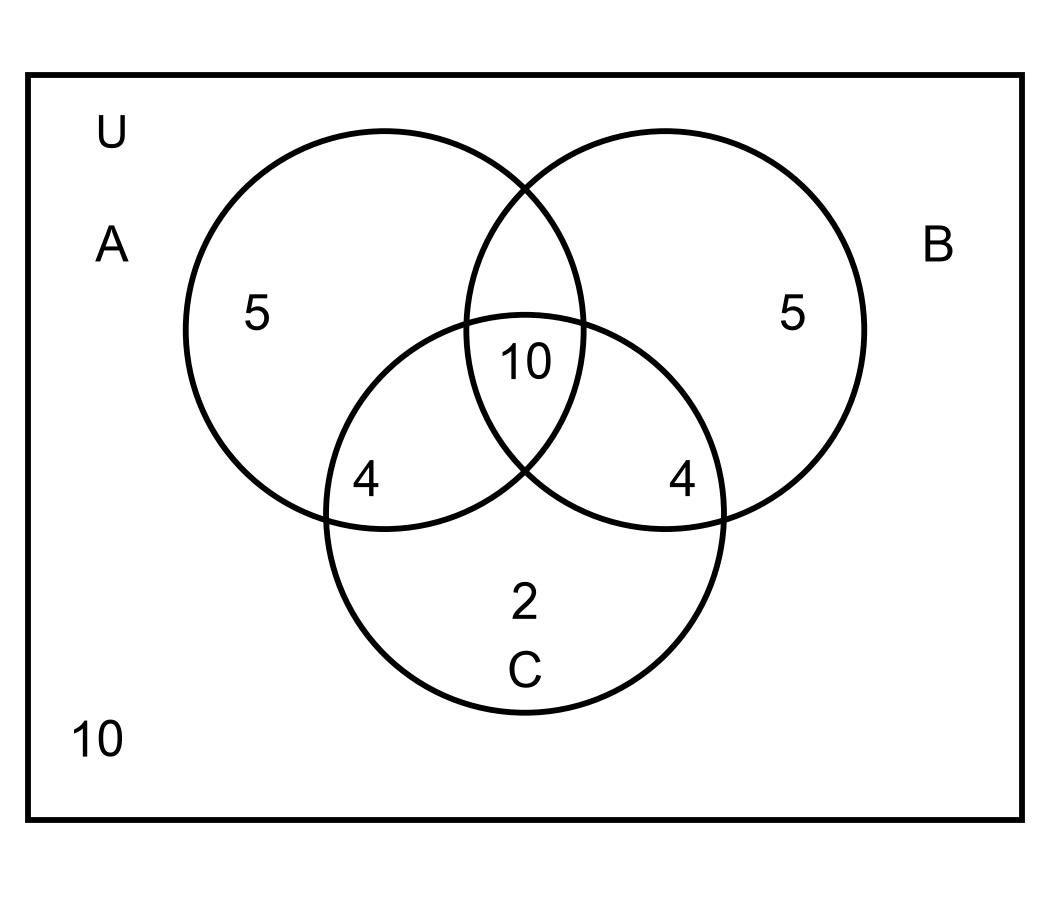
\includegraphics[width=0.38\textwidth]{figures/venn_50_ABC.png}
\end{center}
\step{所以单选物理、化学的人数至多 10 人.}
\step{所以至多选选择物理和化学这两门课程的学生人数至多 $10+10=20$ 人.}
\step{故选 C.}
\solend

\fi

\item 设 $k\geqslant 1,\,k\in\mathbb{N}$，已知集合 $M=\{1,2,3,4,5\}$，若集合 $N_1,N_2,\dots,N_k$ 是集合 $M$ 的 $k$ 个不同非空子集，且 $N_1\cup N_2\cup\dots\cup N_k\neq M$，则 $k$ 的最大值为\mbox{（\quad）.}

\keepwithprev
A. $15$\qquad B. $16$\qquad C. $31$\qquad D. $32$

\ans{A}

\ifanswer
\solbegin
\step{由 $N_1\cup N_2\cup\dots\cup N_k\neq M$ 得所有非空子集的并集缺少集合 $M$ 中至少一个元素.}
\step{假设缺少元素 1，则所有非空子集 $N_i$ 均不含元素 1，即 $N_i$ 是集合 $\{2,3,4,5\}$ 非空子集，集合 $\{2,3,4,5\}$ 的非空子集个数为 $2^4-1=15$，且这些子集 $N_i$ 的并集必不含 1，满足条件.}
\step{假设 $k\geqslant 16$，要满足所有非空子集的并集不等于集合 $M$，必须至少有一个集合 $M$ 中的元素不在任何一个子集中，否则并集就会等于 $M$.}
\step{设这个缺失的元素是 1，那么 $k$ 个非空集都不含元素 1，即每个子集都是集合 $\{2,3,4,5\}$ 的非空子集.}
\step{而集合 $\{2,3,4,5\}$ 只有 $2^4-1=15$ 个不同的非空子集，所以无法从中取出至少 16 个不同的非空子集.}
\step{因此假设不成立，$k$ 必须小于 16.}
\step{所以 $k$ 的最大值为 15，故选 A.}
\solend

\fi

% 注：原卷此题的差集记号是反斜杠 $A\setminus B$（本稿曾误作 $A\vee B$）；$C$ 的集合描述里原卷留了一条
%     待填横线“$x\in A\underline{\quad}B$”（选项按填入的符号分四种情形），本稿曾误作 $\vee\vee$。
%     2026-09-15 回原图核对时已按原卷改回。
\item 对于集合 $A$、$B$，定义 $A\setminus B=\{x\mid x\in A\text{ 且 }x\notin B\}$，则对于集合 $A=\{x\mid x=6n+5,\,n\in\mathbb{N}\}$，$B=\{y\mid y=3m+7,\,m\in\mathbb{N}\}$，$C=\{x\mid x\in A\underline{\hspace{4em}}B\text{ 且 }x<1000\}$，以下说法正确的是\mbox{（\quad）.}

\keepwithprev
A. 若在横线上填入“$\cap$”，则 $C$ 的真子集有 $2^{12}-1$ 个；

B. 若在横线上填入“$\cup$”，则 $C$ 中元素个数大于 250；

C. 若在横线上填入“$\setminus$”，则 $C$ 的非空真子集有 $2^{153}-2$ 个；

% 注：原卷选项 D 作“若在横线上填入“$\cup\complement_{\mathbb N}$”，则 $\complement_{\mathbb N}C$ 中元素个数为 13”；
%     本稿曾把 $\complement_{\mathbb N}$ 抄成 $\varnothing$、把 $\complement_{\mathbb N}C$ 抄成 $C\setminus C$，2026-09-15 回原图核对时已订正。
D. 若在横线上填入“$\cup\complement_{\mathbb{N}}$”，则 $\complement_{\mathbb{N}}C$ 中元素个数为 13.

\ans{B}

\ifanswer
\solbegin
\step{$x=6n+5=3(2n+1)+2$，$y=3m+7=3(m+2)+1$，集合 $A$、$B$ 无公共元素.}
\step{选项 A 中，集合 $C$ 为空集，没有真子集，$A$ 错；}
\step{选项 B 中，由 $6n+5<1000$ 得 $n<165\tfrac{5}{6}$，由 $3m+7<1000$ 得 $m<331$，因此 $C$ 中元素个数为 $166+331=497$，B 正确；}
\step{选项 C 中，$C$ 中元素个数为 166，非空真子集个数为 $2^{166}-2$，C 错；}
% 注：原卷此行作“$\complement_{\mathbb N}C=\complement_{\mathbb N}(A\cup\complement_{\mathbb N}B)
%     =\complement_{\mathbb N}A\cap\complement_{\mathbb N}(\complement_{\mathbb N}B)=\complement_{\mathbb N}A\cap B$，
%     而 $B\subseteq\complement_{\mathbb N}A$”；本稿曾把 $\complement_{\mathbb N}$ 抄成 $C\setminus$，同日已订正。
\step{选项 D 中，$\complement_{\mathbb{N}}C=\complement_{\mathbb{N}}(A\cup\complement_{\mathbb{N}}B)=\complement_{\mathbb{N}}A\cap\complement_{\mathbb{N}}(\complement_{\mathbb{N}}B)=\complement_{\mathbb{N}}A\cap B$，而 $B\subseteq\complement_{\mathbb{N}}A$.}
\step{因此其中元素个数为 331 个，D 错.}
\step{故选 B.}
\solend

\fi
\end{enumerate}

\bigsec{三、解答题}

\begin{enumerate}
\setcounter{enumi}{16}

\item 已知集合 $A=\{x\mid x<-1\text{ 或 }x>4\}$，$B=\{x\mid m+1\leqslant x\leqslant 2m+4\}$.
\begin{enumerate}[label=(\arabic*)]
\item 若 $m=2$，求 $A\cup B$ 和 $\left(\complement_{\R} A\right)\cap B$；
\item 若 $A\cap B=\varnothing$，求 $m$ 的取值范围.
\end{enumerate}

\ans{（1）$A\cup B=\{x\mid x<-1\text{ 或 }x\geqslant 3\}$，$\left(\complement_{\R} A\right)\cap B=\{x\mid 3\leqslant x\leqslant 4\}$；（2）$(-\infty,-3)\cup[-2,0]$}

\ifanswer
\solbegin
\stepm{(1)}{当 $m=2$ 时，集合 $B=\{x\mid 3\leqslant x\leqslant 8\}$.}
\step{又因为 $A=\{x\mid x<-1\text{ 或 }x>4\}$，则 $\complement_{\R}A=\{x\mid -1\leqslant x\leqslant 4\}$，所以 $A\cup B=\{x\mid x<-1\text{ 或 }x\geqslant 3\}$，$\left(\complement_{\R} A\right)\cap B=\{x\mid 3\leqslant x\leqslant 4\}$.}
\stepm{(2)}{因为 $A\cap B=\varnothing$，所以当 $B=\varnothing$ 时，$m+1>2m+4$，解得 $m<-3$ 满足题意；}
\step{当 $B\neq\varnothing$ 时，要满足题意，只需 $\begin{cases}m+1\leqslant 2m+4 \\ m+1\geqslant -1 \\ 2m+4\leqslant 4\end{cases}$，解得 $-2\leqslant m\leqslant 0$.}
\step{综上，实数 $m$ 的范围为 $m<-3$ 或 $-2\leqslant m\leqslant 0$，即 $(-\infty,-3)\cup[-2,0]$.}
\solend

\fi
\ansspace[6]
\item 设集合 $A=\{x\mid x^2+4x=0\}$，$B=\{x\mid x^2+2(a+1)x+a^2-1=0\}$.
\begin{enumerate}[label=(\arabic*)]
\item 写出集合 $A$ 的所有子集；
\item 若 $A\cap B=B$，求实数 $a$ 的取值范围.
\end{enumerate}

\ans{（1）$\{\varnothing,\{0\},\{-4\},\{0,-4\}\}$；（2）$a=1$ 或 $a\leqslant -1$}

\ifanswer
\solbegin
% 注：原卷此行印作“集合 $A$ 的所有子集为 $\varnothing,\{0\},\{-4\},\{0-4\}$”（末项漏逗号、且未加外层花括号）；
%     本稿按规范的列举写法给出，2026-09-15 回原图核对时加注。
\stepm{(1)}{由题意得 $A=\{0,-4\}$，集合 $A$ 的所有子集为 $\varnothing,\{0\},\{-4\},\{0,-4\}$.}
\stepm{(2)}{由 $A\cap B=B$ 得 $B\subseteq A$，所以 $B=\{0\}$ 或 $B=\{-4\}$ 或 $B=\{0,-4\}$ 或 $B=\varnothing$.}
\step{若 $B=\{0\}$ 时，$x^2+2(a+1)x+a^2-1=0$ 有两个相等的根 $0$，则 $\begin{cases}-2(a+1)=0 \\ a^2-1=-4\times(-4)\end{cases}$，解得 $a=-1$.}
\step{若 $B=\{-4\}$ 时，$x^2+2(a+1)x+a^2-1=0$ 有两个相等的根 $-4$，则 $\left\{\begin{matrix}-2(a+1)=-8 \\ a^2-1=-4\times(-4)\end{matrix}\right.$，$a$ 无解.}
\step{若 $B=\{0,-4\}$ 时，$x^2+2(a+1)x+a^2-1=0$ 有两个不相等的根 $0$ 和 $-4$，则 $\begin{cases}-2(a+1)=-4 \\ a^2-1=0\end{cases}$，解得 $a=1$.}
\step{当 $B=\varnothing$ 时，$x^2+2(a+1)x+a^2-1=0$ 无实数根，$\Delta=[2(a+1)]^2-4(a^2-1)=8a+8<0$，得 $a<-1$.}
\step{综上，$a=1$ 或 $a\leqslant -1$.}
\solend

\fi
\ansspace[6]
\item 已知集合 $A=\{x\mid x^2-5x+6=0\}$，$B=\{x\mid mx+1=0\}$，$C=\{x\in\mathbb{N}\mid \sqrt{x}\leqslant 1\}$，且 $A\cup B=A$.
\begin{enumerate}[label=(\arabic*)]
\item 求集合 $M=\{x\mid x\subseteq A\}$ 的真子集的个数；
\item 求实数 $m$ 的值组成的集合；
% 注：原卷本题的定义作“集合 $E=\{x\mid -x\in D,\,2-x^2\notin D\}$”；本稿曾把 $\notin$ 抄成 $\in$
%     （那样 $E=\varnothing$，与答案 $-5$ 冲突），2026-09-15 回原图核对时已订正。
\item 若集合 $D=A\cup C$，定义：集合 $E=\{x\mid -x\in D,\,2-x^2\notin D\}$，求集合 $E$ 中所有元素的和.
\end{enumerate}

\ans{（1）$15$；（2）$\left\{0,-\tfrac{1}{2},-\tfrac{1}{3}\right\}$；（3）$-5$}

\ifanswer
\solbegin
\stepm{(1)}{$A=\{x\mid x^2-5x+6=0\}=\{2,3\}$.}
\step{由 $M=\{x\mid x\subseteq A\}$ 得 $M$ 是 $A$ 的所有子集构成的集合，集合 $A$ 有 2 个元素，故 $A$ 的子集共 $2^2=4$ 个，即 $M$ 含 4 个元素，$M$ 的真子集个数为 $2^4-1=15$.}
\stepm{(2)}{由 (1) 得 $A=\{2,3\}$，集合 $B=\{x\mid mx+1=0\}$.}
\step{由 $A\cup B=A$ 得 $B\subseteq A$，分两种情况：① 当 $m=0$ 时，方程 $mx+1=0$ 无解，$B=\varnothing$，空集是任意集合的子集，符合条件；}
\stepm{②}{当 $m\neq 0$ 时，$B=\{-\tfrac{1}{m}\}$，由 $B\subseteq A$ 得 $-\tfrac{1}{m}=2$ 或 $-\tfrac{1}{m}=3$，解得 $m=-\tfrac{1}{2}$ 或 $m=-\tfrac{1}{3}$.}
\step{实数 $m$ 的取值集合为 $\left\{0,-\tfrac{1}{2},-\tfrac{1}{3}\right\}$.}
\stepm{(3)}{由 (1) 得 $A=\{2,3\}$.}
\step{由 $x\in\mathbb{N}$ 且 $\sqrt{x}\leqslant 1$，得 $x=0$ 或 $x=1$，故 $C=\{0,1\}$.}
\step{所以 $D=A\cup C=\{0,1,2,3\}$.}
\step{由 $-x\in D$ 得 $x$ 的候选值为 $0,-1,-2,-3$.}
\step{由于集合 $E=\{x\mid -x\in D,\,2-x^2\in D\}$，当 $x=0$ 时，$2-x^2=2\in D$，不符合题意；}
\step{当 $x=-1$ 时，$2-x^2=1\in D$，不符合题意；}
\step{当 $x=-2$ 时，$2-x^2=-2\notin D$，符合题意；}
\step{当 $x=-3$ 时，$2-x^2=-7\notin D$，符合题意.}
\step{故 $E=\{-2,-3\}$，所有元素的和为 $-2+(-3)=-5$.}
\solend

\fi
\ansspace[8]
\item 设集合 $M$ 是至少含有两个元素的数集，若 $M$ 中存在两个元素 $x$、$y$ 满足它们的积 $xy\in M$，则称 $M$ 为可积数集.
\begin{enumerate}[label=(\arabic*)]
\item 设集合 $A=\{2,3,5\}$，试判断 $A$ 是否为可积数集？并说明理由；
\item 设集合 $B=\{2,3,4,a\}$，若 $B$ 为可积数集，求实数 $a$ 的取值集合；
\item 设集合 $D=\{x\mid t<x<t+2\}$，若 $D$ 不是可积数集，求实数 $t$ 的取值范围.
\end{enumerate}

% 注：原卷本题【答案】与文末解析的结论都含 $\frac{3}{4}$；本稿曾漏掉 $\frac{3}{4}$
%     （与本稿自己的解析结论不一致），2026-09-15 回原图核对时已订正。
\ans{（1）否；（2）$\left\{0,\tfrac{1}{2},\tfrac{2}{3},\tfrac{3}{4},1,\tfrac{4}{3},\tfrac{3}{2},6,8,12\right\}$；（3）$t\in(-\infty,-2]\cup[2,+\infty)$}

\ifanswer
\solbegin
\stepm{(1)}{因为 $2\times 3=6\notin A$，$2\times 5=10\notin A$，$3\times 5=15\notin A$，所以 $A$ 中任意两个元素的积都不是 $A$ 中的元素，即 $A$ 不是可积数集.}
\stepm{(2)}{若 $B=\{2,3,4,a\}$ 为可积数集，则 $2\times 3=6\in B$，或 $2\times 4=8\in B$ 或 $3\times 4=12\in B$ 或 $2a\in B$ 或 $3a\in B$ 或 $4a\in B$.}
\step{若 $6\in B$，则 $a=6$；}
\step{若 $8\in B$，则 $a=8$；}
\step{若 $12\in B$，则 $a=12$；}
\step{若 $2a\in B$，则 $2a=2$ 或 $2a=3$ 或 $2a=4$ 或 $2a=a$，解得 $a=1$ 或 $a=\tfrac{3}{2}$ 或 $a=2$（舍）或 $a=0$；}
\step{若 $3a\in B$，则 $3a=2$ 或 $3a=3$ 或 $3a=4$ 或 $3a=a$，解得 $a=\tfrac{2}{3}$ 或 $a=1$ 或 $a=\tfrac{4}{3}$ 或 $a=0$；}
\step{若 $4a\in B$，则 $4a=2$ 或 $4a=3$ 或 $4a=4$ 或 $4a=a$，解得 $a=\tfrac{1}{2}$ 或 $a=\tfrac{3}{4}$ 或 $a=1$ 或 $a=0$.}
\step{综上，实数 $a$ 的取值集合为 $\left\{0,\tfrac{1}{2},\tfrac{2}{3},\tfrac{3}{4},1,\tfrac{4}{3},\tfrac{3}{2},6,8,12\right\}$.}
\stepm{(3)}{若 $D=\{x\mid t<x<t+2\}$ 不是可积数集，则 $\forall x,y\in(t,t+2)$，$xy\notin(t,t+2)$.}
\step{当 $t+2\leqslant 0$，即 $t\leqslant -2$ 时，$0\leqslant(t+2)^2<xy<t^2$，此时 $xy\notin D$，满足题意；}
\step{当 $t\geqslant 0$ 时，$0\leqslant t^2<xy<(t+2)^2$，因为 $(t+2)^2>t$，所以若 $xy\notin D$，则 $t^2\geqslant t+2$，即 $t^2-t-2\geqslant 0$，解得 $t\geqslant 2$ 或 $t\leqslant -1$，此时 $t\geqslant 2$ 满足题意；}
% 注：原卷此句作“当 $t<0<t+2$，即 $-2<t<0$ 时，$\exists x=0$，$xy=0\in D$，不满足题意，舍去”；
%     本稿曾把 $\in D$ 抄成 $\notin D$（$-2<t<0$ 时 $0\in(t,t+2)$，确有 $0\in D$），同日已订正。
\step{当 $t<0<t+2$，即 $-2<t<0$ 时，$\exists x=0$，$xy=0\in D$，不满足题意，舍去.}
\step{综上，所求实数 $t$ 的取值范围为 $t\geqslant 2$ 或 $t\leqslant -2$，故 $t\in(-\infty,-2]\cup[2,+\infty)$.}
\solend

\fi
\ansspace[8]
\ansneed{7cm}
\item 已知集合 $A$ 为非空数集，定义：$S=\{x\mid x=a+b,\,a,b\in A\}$，$T=\{x\mid x=|a-b|,a,b\in A\}$（实数 $a$、$b$ 可以相同）.
\begin{enumerate}[label=(\arabic*)]
\item 若集合 $A=\{2,5\}$，直接写出集合 $S$、$T$；
\item 若集合 $A=\{x_1,x_2,x_3,x_4\}$，$x_1<x_2<x_3<x_4$，且 $T=A$，求证：$x_1+x_4=x_3+x_2$；
\item 若集合 $A\subseteq\{x\mid 0\leqslant x\leqslant 2025,\,x\in\mathbb{N}\}$，$S\cap T=\varnothing$，记 $|A|$ 为集合 $A$ 中的元素个数，求 $|A|$ 的最大值.
\end{enumerate}

\ans{（1）$S=\{4,7,10\}$，$T=\{0,3\}$；（2）略；（3）$1350$}

\ifanswer
\solbegin
\stepm{(1)}{$S=\{4,7,10\}$，$T=\{0,3\}$.}
\stepm{(2)}{由集合 $A=\{x_1,x_2,x_3,x_4\}$，$x_1<x_2<x_3<x_4$，则 $T$ 集合的元素在 $0,x_2-x_1,x_3-x_1,x_4-x_1,x_3-x_2,x_4-x_2,x_4-x_3$ 中，且 $0<x_2-x_1<x_3-x_1<x_4-x_1$，$x_3-x_2<x_4-x_2<x_4-x_3$，因为 $A=T$，所以 $A$ 中最大元素 $x_4$ 必在 $T$ 中，而 $x_4-x_1$ 为 7 个元素中的最大者.}
\step{故 $x_4=x_4-x_1$，即 $x_1=0$.}
\step{故 $A=\{0,x_2,x_3,x_4\}$.}
\step{则 $x_3-x_2$、$x_4-x_2$、$x_4-x_3$ 与 $x_2$、$x_3$、$x_4$ 重复.}
\step{而 $0<x_3-x_2<x_3$，故 $x_3-x_2=x_2$，即 $x_3=2x_2$.}
% 注：原卷此句作“而 $0<x_4-x_3<x_4$，故 $x_4-x_3=x_2$ 或 $x_4-x_3=x_3$”；本稿曾把上界写成 $x_3$
%     （那样排除不了 $x_4-x_3=x_3$，与后半句自相矛盾），2026-09-15 回原图核对时已订正。
\step{而 $0<x_4-x_3<x_4$，故 $x_4-x_3=x_2$ 或 $x_4-x_3=x_3$.}
\step{若 $x_4=2x_3=4x_2$，则 $A=\{0,x_2,2x_2,4x_2\}$，$4x_2-x_2=3x_2\notin T$，与题设矛盾.}
\step{故 $x_4-x_3=x_2$，又因为 $x_1=0$，所以 $x_4+x_1=x_3+x_2$.}
% 注：原卷此行作“则 $2a_1<a_1+a_2<a_1+a_3<\cdots<a_1+a_k<a_2+a_k<a_3+a_k<\cdots<a_{k-1}+a_k<2a_k$，
%     所以 $|S|\geqslant 2k-1$，$a_1-a_1<a_2-a_1<a_3-a_1<\cdots<a_k-a_1$，所以 $|T|\geqslant k$”；
%     本稿曾把这个不等式链抄乱（作 $\cdots<a_1+a_k<a_2+a_3<a_k+a_k\leqslant 2a_k$）且把首项写成 $a_i-a_1$，
%     2026-09-15 回原图核对时已订正。
\stepm{(3)}{设 $A=\{a_1,a_2,\dots,a_k\}$ 满足题意，其中 $a_1<a_2<\dots<a_k$，则 $2a_1<a_1+a_2<a_1+a_3<\dots<a_1+a_k<a_2+a_k<a_3+a_k<\dots<a_{k-1}+a_k<2a_k$，所以 $|S|\geqslant 2k-1$，$a_1-a_1<a_2-a_1<a_3-a_1<\dots<a_k-a_1$，所以 $|T|\geqslant k$.}
\step{因为 $S\cap T=\varnothing$，由容斥原理得 $|S\cup T|=|S|+|T|\geqslant 3k-1$.}
\step{$S\cup T$ 中最小的元素为 0，最大的元素为 $2a_k$，$|S\cup T|\leqslant 2a_k+1$，所以 $3k-1\leqslant 2a_k+1\leqslant 2\times 2025+1\,(k\geqslant 1,k\in\mathbb{N})$，即 $3k-1\leqslant 4051$，解得 $k\leqslant 1350\tfrac{2}{3}$.}
\step{实际上 $A=\{676,677,678,\dots,2025\}$ 时满足题意，证明如下：设 $A=\{m,m+1,m+2,\dots,2025\}$，$m\in\mathbb{N}$.}
\step{则 $S=\{2m,2m+1,2m+2,\dots,4050\}$，$T=\{0,1,2,\dots,2025-m\}$.}
\step{由题意得 $2025-m<2m$，即 $m>675$.}
\step{所以 $A=\{676,677,678,\dots,2025\}$ 时满足题意，此时集合 $A$ 中的元素的个数最多.}
\step{综上所述，集合 $A$ 中元素的个数的最大值是 1350.}
\solend

\fi
\ansspace*[10]
\end{enumerate}

\end{document}"
%
% 原始材料是微信公众号图文（“魔都数学加油站”，作者署名“破晓”），正文为 11 张 PNG 页
% （1080×1527）；卷面上的粉色斜水印“魔都数学加油站”属水印，未录入。原文本身就是一份
% **讲评版**——题下直接印出【答案】或【解析】，本稿把这些答案与解析移到答案版，试卷版即
% 一张干净的空卷。
%
% 与原卷的排版差异（均已在 README“说明”中交代）：
%   ① 原文自**第 3 题**起（第 1、2 题未在该文发布），源码里以 \setcounter{enumi}{2} 起编；
%   ② 原卷本就印有分节标题“一、填空题”“二、选择题”“三、解答题”（已在原图上逐页放大
%      核对过），本稿照原卷分节，只把标题改排成全稿统一的“大节标题”样式；
%   ③ 原卷的实数集、整数集符号作正体 $R$（第 7 题）、$Z$（第 11 题），本稿按全稿惯例统一
%      写作 $\R$、$\Z$；
%   ④ 第 14 题【解析】里的 Venn 图取自原卷截图（`figures/venn_50_ABC.png`，4× LANCZOS
%      放大），未用 TikZ 重绘.

\documentclass[a4paper,11pt]{article}
\usepackage{common}

\begin{document}

\examtitlest{2026--2027 学年度交附闵行高一上周练 1}{集合与常用逻辑用语}

\bigsec{一、填空题}

\begin{enumerate}
\setcounter{enumi}{2}

\item 已知集合 $A=\{2,14,x^2+5\}$，$B=\{2,2x\}$，若 $A\cap B=B$，则实数 $x=$ \blankline[2em].

\ans{$7$}

\ifanswer
\solbegin
\step{因为 $A\cap B=B$，所以 $B\subseteq A$，所以 $2x=14$ 或 $x^2+5=2x$.}
\step{$2x=14$ 时，$x=7$，此时 $A=\{2,14,54\}$，$B=\{2,14\}$ 满足题意；}
\step{$x^2+5=2x$ 时，$(x-1)^2+4=0$，无解.}
\step{所以 $x=7$.}
\solend

\fi
\item 设集合 $A=\{y\mid y=x^2-1\}$，$B=\{(x,y)\mid y=x\}$，则 $A\cap B=$ \blankline[2em].

\ans{$\varnothing$}

\item 若集合 $\{0,-1,2a\}=\{a-1,-|a|,a+1\}$，实数 $a$ 的值为 \blankline[2em].

\ans{$\pm 1$}

\ifanswer
\solbegin
\step{令 $A=\{0,-1,2a\}$，$B=\{a-1,-|a|,a+1\}$，因为 $\{0,-1,2a\}=\{a-1,-|a|,a+1\}$，若 $a-1=0$，则 $a=1$，则 $A=\{0,-1,2\}$，$B=\{0,-1,2\}$，满足要求；}
\step{若 $-|a|=0$，则 $a=0$，则 $A=\{0,-1,0\}$，不满足集合元素的互异性；}
\step{若 $a+1=0$，则 $a=-1$，则 $A=\{0,-1,-2\}$，$B=\{0,-1,-2\}$，满足要求.}
\step{故实数 $a$ 的值为 $\pm 1$.}
\solend

\fi
\item 已知全集 $U=(-4,3]$，$A=\{x\in U\mid x^2+2x-8=0\}$，$B=\{x\in U\mid -3<1-2x\leqslant 5\}$，则 $\left(\complement_U B\right)\cap A=$ \blankline[2em].

\ans{$\{2\}$}

\item 已知集合 $A=\{x\mid 1-a\leqslant x\leqslant 1+a,\,a\in\R\}$ 中只有一个整数元素，则实数 $a$ 的取值范围为 \blankline[2em].

\ans{$[0,1)$}

\ifanswer
\solbegin
\step{集合 $A=\{x\mid 1-a\leqslant x\leqslant 1+a,\,a\in\R\}$ 中只有一个整数元素，则 $A\neq\varnothing,\,1-a\leqslant 1+a$，即 $a\geqslant 0$，此时 $1\in A$，故 $\begin{cases}1+a<2 \\ 1-a>0\end{cases}$，解得 $a<1$.}
\step{故 $a\in[0,1)$.}
\solend

\fi
\item 已知全集 $U=\{x\in\mathbb{N}\mid x\leqslant 9\}$，$A\cap B=\{3\}$，$\overline{A}\cap B=\{4,6,8\}$，$A\cap\overline{B}=\{1,5\}$，则 $\overline{A}=$ \blankline[2em].

\ans{$\{0,2,4,6,7,8,9\}$}

\ifanswer
\solbegin
\step{由题意得 $U=\{x\in\mathbb{N}\mid x\leqslant 9\}=\{0,1,2,3,4,5,6,7,8,9\}$，$A\cap B=\{3\}$ 得 $A$、$B$ 中含有元素 $3$；}
\step{$\overline{A}\cap B=\{4,6,8\}$ 得 $B$ 中含有 $4$、$6$、$8$，集合 $A$ 中不含 $4$、$6$、$8$；}
\step{$A\cap\overline{B}=\{1,5\}$ 得 $A$ 含有 $1$、$5$，集合 $B$ 不含 $1$、$5$.}
\step{对于 $0$，假设集合 $A$ 中含有 $0$，由 $A\cap B=\{3\}$ 得 $B$ 不含 $0$，则 $A\cap\overline{B}$ 必含元素 $0$，与 $A\cap\overline{B}=\{1,5\}$ 矛盾.}
\step{同理可得集合 $A$ 中不含元素 $2$、$7$、$9$.}
\step{综上所述，$A=\{1,3,5\}$.}
\step{故 $\overline{A}=\{0,2,4,6,7,8,9\}$.}
\solend

\fi
\item 已知一个有四个数字元素的集合 $S$，$S$ 的所有子集的元素和（空集的元素和认为是 0）的总和为 16208，则 $S$ 的元素之和等于 \blankline[2em].

\ans{$2026$}

\ifanswer
\solbegin
\step{设 $S=\{a_1,a_2,a_3,a_4\}$，$S$ 的每个元素在所有子集中均出现 $2^3$ 次，故 $(a_1+a_2+a_3+a_4)\cdot 2^3=16208$，所以 $a_1+a_2+a_3+a_4=2026$，故 $S$ 的元素之和等于 2026.}
\solend

\fi
\item 已知集合 $M=\{x\in\mathbb{N}\mid 1\leqslant x\leqslant 12\}$，集合 $A_1$、$A_2$、$A_3$ 满足：① 每个集合都恰有 4 个元素；② $A_1\cup A_2\cup A_3=M$. 集合 $A_i\,(i=1,2,3)$ 中元素的最大值与最小值之和称为集合 $A_i$ 的特征数，记为 $X_i\,(i=1,2,3)$，则 $X_1+X_2+X_3$ 的最大值与最小值的积为 \blankline[2em].

\ans{$1485$}

\ifanswer
\solbegin
\step{集合 $M=\{x\in\mathbb{N}\mid 1\leqslant x\leqslant 12\}$ 中最小值为 1，最大值为 12.}
% 注：原卷此处印作“则 $A_1=13$”（原卷笔误，按上下文应为 $X_1=13$），本稿按 $X_1$ 规范，2026-09-15 回原图核对时加注。
\stepm{①}{若使 $X_1+X_2+X_3$ 取得最大值，不妨设 $A_1=\{1,2,3,12\}$，则 $X_1=13$，则剩余的数中最小值是 4，最大值是 11，令 $A_2=\{4,5,6,11\}$，则 $X_2=15$，则 $A_3=\{7,8,9,10\}$，$X_3=17$，则 $X_1+X_2+X_3$ 的最大值为 $13+15+17=45$；}
\stepm{②}{若使 $X_1+X_2+X_3$ 取得最小值，则 $A_1=\{1,4,5,6\}$，则 $X_1=7$，令 $A_2=\{2,7,8,9\}$，则 $X_2=11$，则 $A_3=\{3,10,11,12\}$，$X_3=15$，则此时 $X_1+X_2+X_3$ 的最小值为 $7+11+15=33$.}
\step{故 $X_1+X_2+X_3$ 的最大值与最小值的积为 $45\times 33=1485$.}
\solend

\fi
\item 对于集合 $M=\{a\mid a=x^2-y^2,\,x\in\Z,\,y\in\Z\}$，给出如下三个结论：

① 如果 $P=\{b\mid b=2n+1,\,n\in\Z\}$，那么 $P\subseteq M$；

% 注：原卷此条作“如果 $c=4n+2$，$n\in\Z$，那么 $c\notin M$”；本稿曾把 $\notin$ 抄成 $\in$
%     （那样②为假，与本卷答案 ①②③ 冲突），2026-09-15 回原图核对时已订正。
② 如果 $c=4n+2$，$n\in\Z$，那么 $c\notin M$；

③ 如果 $a_1\in M$，$a_2\in M$，那么 $a_1a_2\in M$. 其中正确结论的序号是 \blankline[2em].

\ans{①②③}

\ifanswer
\solbegin
\stepm{①}{由已知 $b=2n+1,\,n\in\Z$，则恒有 $2n+1=(n+1)^2-n^2,\,n\in\Z$，所以 $2n+1\in M$，所以 $P\subseteq M$，所以①正确；}
\stepm{②}{元素 $c=4n+2,\,n\in\Z$，若 $4n+2\in M$，则存在 $x$、$y\in\Z$ 使得 $x^2-y^2=4n+2$，所以 $4n+2=(x+y)(x-y)$，则 $x+y$ 与 $x-y$ 同奇或同偶.}
\step{若 $x+y$ 与 $x-y$ 都是奇数，则 $(x+y)(x-y)$ 为奇数，而 $4n+2$ 是偶数；}
\step{若 $x+y$ 和 $x-y$ 都是偶数，则 $(x+y)(x-y)$ 能被 4 整除，而 $4n+2$ 不能被 4 整除.}
\step{所以 $4n+2\notin M$，即 $c\notin M$，故②正确；}
\stepm{③}{因为 $a_1$、$a_2\in M$，则 $a_1a_2$ 还是整数，所以 $a_1a_2\in M$，故③正确.}
\step{故正确的是①②③.}
\solend

\fi
\item 用 $C(A)$ 表示非空集合 $A$ 中的元素的个数，定义 $A*B=|C(A)-C(B)|$，若 $A=\{x\mid x^2-2024x-2025=0\}$，$B=\{x\mid (2x^2+ax)(x^2+2ax+6)=0\}$，若 $A*B=1$，则 $a$ 的所有可能取值构成集合 $M$，则 $C(M)=$ \blankline[2em].

\ans{$5$}

\ifanswer
\solbegin
\step{$x^2-2024x-2025=0$ 得 $x=2025$ 或 $x=-1$，即 $C(A)=2$，因为 $A*B=|C(A)-C(B)|=1$，所以 $C(B)=3$ 或 $C(B)=1$.}
\step{方程 $(2x^2+ax)(x^2+2ax+6)=0$ 化为 $x(2x+a)(x^2+2ax+6)=0$.}
\step{当 $a=0$ 时，方程化为 $2x^3(x^2+6)=0$，解得 $x=0$，所以 $B=\{0\}$，$C(B)=1$，符合题意.}
\step{当 $a\neq 0$ 时，方程化为 $x=0$ 或 $x=-\tfrac{a}{2}$ 或 $x^2+2ax+6=0$.}
\step{因为 $0\neq -\tfrac{a}{2}$，$C(B)\neq 1$，故只有 $C(B)=3$.}
\step{故 $x^2+2ax+6=0$ 有两个相等的非零实数根，所以 $\Delta=4a^2-4\times 6=0$，解得 $a=\pm\sqrt{6}$，符合题意.}
\step{当 $x^2+2ax+6=0$ 有两个不相等实根，设 $x_1$、$x_2$，若 $x_1=-\tfrac{a}{2}$，由韦达定理得 $\begin{cases}x_1+x_2=-2a \\ x_1x_2=6\end{cases}$，% 注：原卷作“得 $x_2=-\frac{3a}{2}$”（由 $x_1+x_2=-2a$、$x_1=-\frac{a}{2}$ 得 $x_2=-\frac{3a}{2}$）；
%     本稿曾漏掉负号，2026-09-15 回原图核对时已订正。
得 $x_2=-\tfrac{3a}{2}$，$-\tfrac{a}{2}\cdot(-\tfrac{3a}{2})=\tfrac{3a^2}{4}=6$，解得 $a=\pm 2\sqrt{2}$，符合题意.}
\step{综上所述，$M=\{0,\sqrt{6},-\sqrt{6},2\sqrt{2},-2\sqrt{2}\}$，所以 $C(M)=5$.}
\solend

\fi
\end{enumerate}

\bigsec{二、选择题}

\begin{enumerate}
\setcounter{enumi}{12}

\item 已知集合 $A=\{1,2,3,4,5\}$，$B=\{x\mid \tfrac{x-1}{2}\in\Z,\,x\in A\}$，则集合 $B$ 的真子集个数为\mbox{（\quad）.}

\keepwithprev
A. $3$\qquad B. $5$\qquad C. $7$\qquad D. $15$

\ans{C}

\ifanswer
\solbegin
\step{已知集合 $A=\{1,2,3,4,5\}$，$B=\{x\mid\tfrac{x-1}{2}\in\Z,\,x\in A\}$.}
\step{因为 $\tfrac{x-1}{2}\in\Z$，所以 $x$ 为奇数，所以 $B=\{1,3,5\}$.}
\step{所以集合 $B$ 中有 3 个元素，所以集合 $B$ 的真子集个数为 $2^3-1=7$.}
\step{故选 C.}
\solend

\fi

\item 高一二班共有学生 50 人，每名学生要从物理、化学、生物、历史、地理、政治这六门课程中选择三门课程进行学习. 已知选择物理、化学、生物的学生各有至少 20 人，这三门课程都不选的有 10 人，这三门课程都选的有 10 人，在这三门课程中选择任意两门课程的都至少有 14 人，物理、化学只选一科的学生都至少 5 人，那么选择物理和化学这两门课程的学生人数至多\mbox{（\quad）.}

\keepwithprev
A. $18$\qquad B. $19$\qquad C. $20$\qquad D. $21$

\ans{C}

\ifanswer
\solbegin
\step{可以把学生 50 人看作一个集合 $U$，选择物理的人数组成集合 $A$，选择化学的人数组成集合 $B$，选择生物的人数组成集合 $C$.}
\step{要使选择物理和化学这两门课程的学生人数最多，除这三门课程都不选的有 10 人，这三门课程都选的有 10 人，则其他科选择人数均为最少，因为物理、化学只选一科的学生都至少 5 人，即得到单选物理的最少 5 人，单选化学的最少 5 人.}
\step{因为在这三门课程中选择任意两门课程的都至少有 14 人，单选化学、生物的最少 4 人，单选物理、生物的最少 4 人.}
\step{因为选择物理、化学、生物的学生各有至少 20 人，所以单选生物的最少 2 人.}
\step{以上人数最少 30 人，可作出如图所示的韦恩图：}
% 注：原卷此处印有一张韦恩图（三个圆 $A$、$B$、$C$，$A$ 独有 5、$B$ 独有 5、三集合公共 10、
%     $A\cap C$ 独有 4、$B\cap C$ 独有 4、$C$ 独有 2、三集合之外 10）；本稿此前漏排此图而正文仍作
%     “如图”，2026-09-15 回原图核对时按原卷截图补入（见 figures/venn_50_ABC.png）。
\begin{center}
% 插图取自原卷截图（裁去截图残影后 4× LANCZOS 放大），不用 TikZ 手绘
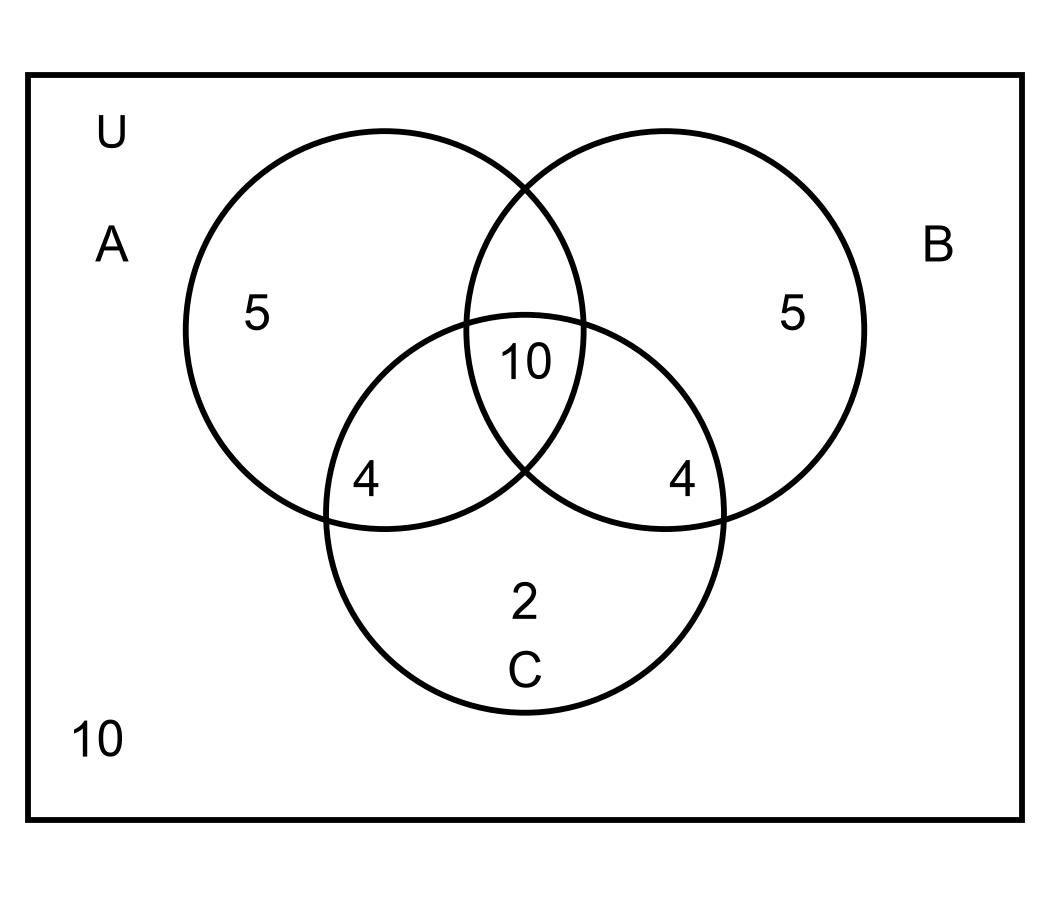
\includegraphics[width=0.38\textwidth]{figures/venn_50_ABC.png}
\end{center}
\step{所以单选物理、化学的人数至多 10 人.}
\step{所以至多选选择物理和化学这两门课程的学生人数至多 $10+10=20$ 人.}
\step{故选 C.}
\solend

\fi

\item 设 $k\geqslant 1,\,k\in\mathbb{N}$，已知集合 $M=\{1,2,3,4,5\}$，若集合 $N_1,N_2,\dots,N_k$ 是集合 $M$ 的 $k$ 个不同非空子集，且 $N_1\cup N_2\cup\dots\cup N_k\neq M$，则 $k$ 的最大值为\mbox{（\quad）.}

\keepwithprev
A. $15$\qquad B. $16$\qquad C. $31$\qquad D. $32$

\ans{A}

\ifanswer
\solbegin
\step{由 $N_1\cup N_2\cup\dots\cup N_k\neq M$ 得所有非空子集的并集缺少集合 $M$ 中至少一个元素.}
\step{假设缺少元素 1，则所有非空子集 $N_i$ 均不含元素 1，即 $N_i$ 是集合 $\{2,3,4,5\}$ 非空子集，集合 $\{2,3,4,5\}$ 的非空子集个数为 $2^4-1=15$，且这些子集 $N_i$ 的并集必不含 1，满足条件.}
\step{假设 $k\geqslant 16$，要满足所有非空子集的并集不等于集合 $M$，必须至少有一个集合 $M$ 中的元素不在任何一个子集中，否则并集就会等于 $M$.}
\step{设这个缺失的元素是 1，那么 $k$ 个非空集都不含元素 1，即每个子集都是集合 $\{2,3,4,5\}$ 的非空子集.}
\step{而集合 $\{2,3,4,5\}$ 只有 $2^4-1=15$ 个不同的非空子集，所以无法从中取出至少 16 个不同的非空子集.}
\step{因此假设不成立，$k$ 必须小于 16.}
\step{所以 $k$ 的最大值为 15，故选 A.}
\solend

\fi

% 注：原卷此题的差集记号是反斜杠 $A\setminus B$（本稿曾误作 $A\vee B$）；$C$ 的集合描述里原卷留了一条
%     待填横线“$x\in A\underline{\quad}B$”（选项按填入的符号分四种情形），本稿曾误作 $\vee\vee$。
%     2026-09-15 回原图核对时已按原卷改回。
\item 对于集合 $A$、$B$，定义 $A\setminus B=\{x\mid x\in A\text{ 且 }x\notin B\}$，则对于集合 $A=\{x\mid x=6n+5,\,n\in\mathbb{N}\}$，$B=\{y\mid y=3m+7,\,m\in\mathbb{N}\}$，$C=\{x\mid x\in A\underline{\hspace{4em}}B\text{ 且 }x<1000\}$，以下说法正确的是\mbox{（\quad）.}

\keepwithprev
A. 若在横线上填入“$\cap$”，则 $C$ 的真子集有 $2^{12}-1$ 个；

B. 若在横线上填入“$\cup$”，则 $C$ 中元素个数大于 250；

C. 若在横线上填入“$\setminus$”，则 $C$ 的非空真子集有 $2^{153}-2$ 个；

% 注：原卷选项 D 作“若在横线上填入“$\cup\complement_{\mathbb N}$”，则 $\complement_{\mathbb N}C$ 中元素个数为 13”；
%     本稿曾把 $\complement_{\mathbb N}$ 抄成 $\varnothing$、把 $\complement_{\mathbb N}C$ 抄成 $C\setminus C$，2026-09-15 回原图核对时已订正。
D. 若在横线上填入“$\cup\complement_{\mathbb{N}}$”，则 $\complement_{\mathbb{N}}C$ 中元素个数为 13.

\ans{B}

\ifanswer
\solbegin
\step{$x=6n+5=3(2n+1)+2$，$y=3m+7=3(m+2)+1$，集合 $A$、$B$ 无公共元素.}
\step{选项 A 中，集合 $C$ 为空集，没有真子集，$A$ 错；}
\step{选项 B 中，由 $6n+5<1000$ 得 $n<165\tfrac{5}{6}$，由 $3m+7<1000$ 得 $m<331$，因此 $C$ 中元素个数为 $166+331=497$，B 正确；}
\step{选项 C 中，$C$ 中元素个数为 166，非空真子集个数为 $2^{166}-2$，C 错；}
% 注：原卷此行作“$\complement_{\mathbb N}C=\complement_{\mathbb N}(A\cup\complement_{\mathbb N}B)
%     =\complement_{\mathbb N}A\cap\complement_{\mathbb N}(\complement_{\mathbb N}B)=\complement_{\mathbb N}A\cap B$，
%     而 $B\subseteq\complement_{\mathbb N}A$”；本稿曾把 $\complement_{\mathbb N}$ 抄成 $C\setminus$，同日已订正。
\step{选项 D 中，$\complement_{\mathbb{N}}C=\complement_{\mathbb{N}}(A\cup\complement_{\mathbb{N}}B)=\complement_{\mathbb{N}}A\cap\complement_{\mathbb{N}}(\complement_{\mathbb{N}}B)=\complement_{\mathbb{N}}A\cap B$，而 $B\subseteq\complement_{\mathbb{N}}A$.}
\step{因此其中元素个数为 331 个，D 错.}
\step{故选 B.}
\solend

\fi
\end{enumerate}

\bigsec{三、解答题}

\begin{enumerate}
\setcounter{enumi}{16}

\item 已知集合 $A=\{x\mid x<-1\text{ 或 }x>4\}$，$B=\{x\mid m+1\leqslant x\leqslant 2m+4\}$.
\begin{enumerate}[label=(\arabic*)]
\item 若 $m=2$，求 $A\cup B$ 和 $\left(\complement_{\R} A\right)\cap B$；
\item 若 $A\cap B=\varnothing$，求 $m$ 的取值范围.
\end{enumerate}

\ans{（1）$A\cup B=\{x\mid x<-1\text{ 或 }x\geqslant 3\}$，$\left(\complement_{\R} A\right)\cap B=\{x\mid 3\leqslant x\leqslant 4\}$；（2）$(-\infty,-3)\cup[-2,0]$}

\ifanswer
\solbegin
\stepm{(1)}{当 $m=2$ 时，集合 $B=\{x\mid 3\leqslant x\leqslant 8\}$.}
\step{又因为 $A=\{x\mid x<-1\text{ 或 }x>4\}$，则 $\complement_{\R}A=\{x\mid -1\leqslant x\leqslant 4\}$，所以 $A\cup B=\{x\mid x<-1\text{ 或 }x\geqslant 3\}$，$\left(\complement_{\R} A\right)\cap B=\{x\mid 3\leqslant x\leqslant 4\}$.}
\stepm{(2)}{因为 $A\cap B=\varnothing$，所以当 $B=\varnothing$ 时，$m+1>2m+4$，解得 $m<-3$ 满足题意；}
\step{当 $B\neq\varnothing$ 时，要满足题意，只需 $\begin{cases}m+1\leqslant 2m+4 \\ m+1\geqslant -1 \\ 2m+4\leqslant 4\end{cases}$，解得 $-2\leqslant m\leqslant 0$.}
\step{综上，实数 $m$ 的范围为 $m<-3$ 或 $-2\leqslant m\leqslant 0$，即 $(-\infty,-3)\cup[-2,0]$.}
\solend

\fi
\ansspace[6]
\item 设集合 $A=\{x\mid x^2+4x=0\}$，$B=\{x\mid x^2+2(a+1)x+a^2-1=0\}$.
\begin{enumerate}[label=(\arabic*)]
\item 写出集合 $A$ 的所有子集；
\item 若 $A\cap B=B$，求实数 $a$ 的取值范围.
\end{enumerate}

\ans{（1）$\{\varnothing,\{0\},\{-4\},\{0,-4\}\}$；（2）$a=1$ 或 $a\leqslant -1$}

\ifanswer
\solbegin
% 注：原卷此行印作“集合 $A$ 的所有子集为 $\varnothing,\{0\},\{-4\},\{0-4\}$”（末项漏逗号、且未加外层花括号）；
%     本稿按规范的列举写法给出，2026-09-15 回原图核对时加注。
\stepm{(1)}{由题意得 $A=\{0,-4\}$，集合 $A$ 的所有子集为 $\varnothing,\{0\},\{-4\},\{0,-4\}$.}
\stepm{(2)}{由 $A\cap B=B$ 得 $B\subseteq A$，所以 $B=\{0\}$ 或 $B=\{-4\}$ 或 $B=\{0,-4\}$ 或 $B=\varnothing$.}
\step{若 $B=\{0\}$ 时，$x^2+2(a+1)x+a^2-1=0$ 有两个相等的根 $0$，则 $\begin{cases}-2(a+1)=0 \\ a^2-1=-4\times(-4)\end{cases}$，解得 $a=-1$.}
\step{若 $B=\{-4\}$ 时，$x^2+2(a+1)x+a^2-1=0$ 有两个相等的根 $-4$，则 $\left\{\begin{matrix}-2(a+1)=-8 \\ a^2-1=-4\times(-4)\end{matrix}\right.$，$a$ 无解.}
\step{若 $B=\{0,-4\}$ 时，$x^2+2(a+1)x+a^2-1=0$ 有两个不相等的根 $0$ 和 $-4$，则 $\begin{cases}-2(a+1)=-4 \\ a^2-1=0\end{cases}$，解得 $a=1$.}
\step{当 $B=\varnothing$ 时，$x^2+2(a+1)x+a^2-1=0$ 无实数根，$\Delta=[2(a+1)]^2-4(a^2-1)=8a+8<0$，得 $a<-1$.}
\step{综上，$a=1$ 或 $a\leqslant -1$.}
\solend

\fi
\ansspace[6]
\item 已知集合 $A=\{x\mid x^2-5x+6=0\}$，$B=\{x\mid mx+1=0\}$，$C=\{x\in\mathbb{N}\mid \sqrt{x}\leqslant 1\}$，且 $A\cup B=A$.
\begin{enumerate}[label=(\arabic*)]
\item 求集合 $M=\{x\mid x\subseteq A\}$ 的真子集的个数；
\item 求实数 $m$ 的值组成的集合；
% 注：原卷本题的定义作“集合 $E=\{x\mid -x\in D,\,2-x^2\notin D\}$”；本稿曾把 $\notin$ 抄成 $\in$
%     （那样 $E=\varnothing$，与答案 $-5$ 冲突），2026-09-15 回原图核对时已订正。
\item 若集合 $D=A\cup C$，定义：集合 $E=\{x\mid -x\in D,\,2-x^2\notin D\}$，求集合 $E$ 中所有元素的和.
\end{enumerate}

\ans{（1）$15$；（2）$\left\{0,-\tfrac{1}{2},-\tfrac{1}{3}\right\}$；（3）$-5$}

\ifanswer
\solbegin
\stepm{(1)}{$A=\{x\mid x^2-5x+6=0\}=\{2,3\}$.}
\step{由 $M=\{x\mid x\subseteq A\}$ 得 $M$ 是 $A$ 的所有子集构成的集合，集合 $A$ 有 2 个元素，故 $A$ 的子集共 $2^2=4$ 个，即 $M$ 含 4 个元素，$M$ 的真子集个数为 $2^4-1=15$.}
\stepm{(2)}{由 (1) 得 $A=\{2,3\}$，集合 $B=\{x\mid mx+1=0\}$.}
\step{由 $A\cup B=A$ 得 $B\subseteq A$，分两种情况：① 当 $m=0$ 时，方程 $mx+1=0$ 无解，$B=\varnothing$，空集是任意集合的子集，符合条件；}
\stepm{②}{当 $m\neq 0$ 时，$B=\{-\tfrac{1}{m}\}$，由 $B\subseteq A$ 得 $-\tfrac{1}{m}=2$ 或 $-\tfrac{1}{m}=3$，解得 $m=-\tfrac{1}{2}$ 或 $m=-\tfrac{1}{3}$.}
\step{实数 $m$ 的取值集合为 $\left\{0,-\tfrac{1}{2},-\tfrac{1}{3}\right\}$.}
\stepm{(3)}{由 (1) 得 $A=\{2,3\}$.}
\step{由 $x\in\mathbb{N}$ 且 $\sqrt{x}\leqslant 1$，得 $x=0$ 或 $x=1$，故 $C=\{0,1\}$.}
\step{所以 $D=A\cup C=\{0,1,2,3\}$.}
\step{由 $-x\in D$ 得 $x$ 的候选值为 $0,-1,-2,-3$.}
\step{由于集合 $E=\{x\mid -x\in D,\,2-x^2\in D\}$，当 $x=0$ 时，$2-x^2=2\in D$，不符合题意；}
\step{当 $x=-1$ 时，$2-x^2=1\in D$，不符合题意；}
\step{当 $x=-2$ 时，$2-x^2=-2\notin D$，符合题意；}
\step{当 $x=-3$ 时，$2-x^2=-7\notin D$，符合题意.}
\step{故 $E=\{-2,-3\}$，所有元素的和为 $-2+(-3)=-5$.}
\solend

\fi
\ansspace[8]
\item 设集合 $M$ 是至少含有两个元素的数集，若 $M$ 中存在两个元素 $x$、$y$ 满足它们的积 $xy\in M$，则称 $M$ 为可积数集.
\begin{enumerate}[label=(\arabic*)]
\item 设集合 $A=\{2,3,5\}$，试判断 $A$ 是否为可积数集？并说明理由；
\item 设集合 $B=\{2,3,4,a\}$，若 $B$ 为可积数集，求实数 $a$ 的取值集合；
\item 设集合 $D=\{x\mid t<x<t+2\}$，若 $D$ 不是可积数集，求实数 $t$ 的取值范围.
\end{enumerate}

% 注：原卷本题【答案】与文末解析的结论都含 $\frac{3}{4}$；本稿曾漏掉 $\frac{3}{4}$
%     （与本稿自己的解析结论不一致），2026-09-15 回原图核对时已订正。
\ans{（1）否；（2）$\left\{0,\tfrac{1}{2},\tfrac{2}{3},\tfrac{3}{4},1,\tfrac{4}{3},\tfrac{3}{2},6,8,12\right\}$；（3）$t\in(-\infty,-2]\cup[2,+\infty)$}

\ifanswer
\solbegin
\stepm{(1)}{因为 $2\times 3=6\notin A$，$2\times 5=10\notin A$，$3\times 5=15\notin A$，所以 $A$ 中任意两个元素的积都不是 $A$ 中的元素，即 $A$ 不是可积数集.}
\stepm{(2)}{若 $B=\{2,3,4,a\}$ 为可积数集，则 $2\times 3=6\in B$，或 $2\times 4=8\in B$ 或 $3\times 4=12\in B$ 或 $2a\in B$ 或 $3a\in B$ 或 $4a\in B$.}
\step{若 $6\in B$，则 $a=6$；}
\step{若 $8\in B$，则 $a=8$；}
\step{若 $12\in B$，则 $a=12$；}
\step{若 $2a\in B$，则 $2a=2$ 或 $2a=3$ 或 $2a=4$ 或 $2a=a$，解得 $a=1$ 或 $a=\tfrac{3}{2}$ 或 $a=2$（舍）或 $a=0$；}
\step{若 $3a\in B$，则 $3a=2$ 或 $3a=3$ 或 $3a=4$ 或 $3a=a$，解得 $a=\tfrac{2}{3}$ 或 $a=1$ 或 $a=\tfrac{4}{3}$ 或 $a=0$；}
\step{若 $4a\in B$，则 $4a=2$ 或 $4a=3$ 或 $4a=4$ 或 $4a=a$，解得 $a=\tfrac{1}{2}$ 或 $a=\tfrac{3}{4}$ 或 $a=1$ 或 $a=0$.}
\step{综上，实数 $a$ 的取值集合为 $\left\{0,\tfrac{1}{2},\tfrac{2}{3},\tfrac{3}{4},1,\tfrac{4}{3},\tfrac{3}{2},6,8,12\right\}$.}
\stepm{(3)}{若 $D=\{x\mid t<x<t+2\}$ 不是可积数集，则 $\forall x,y\in(t,t+2)$，$xy\notin(t,t+2)$.}
\step{当 $t+2\leqslant 0$，即 $t\leqslant -2$ 时，$0\leqslant(t+2)^2<xy<t^2$，此时 $xy\notin D$，满足题意；}
\step{当 $t\geqslant 0$ 时，$0\leqslant t^2<xy<(t+2)^2$，因为 $(t+2)^2>t$，所以若 $xy\notin D$，则 $t^2\geqslant t+2$，即 $t^2-t-2\geqslant 0$，解得 $t\geqslant 2$ 或 $t\leqslant -1$，此时 $t\geqslant 2$ 满足题意；}
% 注：原卷此句作“当 $t<0<t+2$，即 $-2<t<0$ 时，$\exists x=0$，$xy=0\in D$，不满足题意，舍去”；
%     本稿曾把 $\in D$ 抄成 $\notin D$（$-2<t<0$ 时 $0\in(t,t+2)$，确有 $0\in D$），同日已订正。
\step{当 $t<0<t+2$，即 $-2<t<0$ 时，$\exists x=0$，$xy=0\in D$，不满足题意，舍去.}
\step{综上，所求实数 $t$ 的取值范围为 $t\geqslant 2$ 或 $t\leqslant -2$，故 $t\in(-\infty,-2]\cup[2,+\infty)$.}
\solend

\fi
\ansspace[8]
\ansneed{7cm}
\item 已知集合 $A$ 为非空数集，定义：$S=\{x\mid x=a+b,\,a,b\in A\}$，$T=\{x\mid x=|a-b|,a,b\in A\}$（实数 $a$、$b$ 可以相同）.
\begin{enumerate}[label=(\arabic*)]
\item 若集合 $A=\{2,5\}$，直接写出集合 $S$、$T$；
\item 若集合 $A=\{x_1,x_2,x_3,x_4\}$，$x_1<x_2<x_3<x_4$，且 $T=A$，求证：$x_1+x_4=x_3+x_2$；
\item 若集合 $A\subseteq\{x\mid 0\leqslant x\leqslant 2025,\,x\in\mathbb{N}\}$，$S\cap T=\varnothing$，记 $|A|$ 为集合 $A$ 中的元素个数，求 $|A|$ 的最大值.
\end{enumerate}

\ans{（1）$S=\{4,7,10\}$，$T=\{0,3\}$；（2）略；（3）$1350$}

\ifanswer
\solbegin
\stepm{(1)}{$S=\{4,7,10\}$，$T=\{0,3\}$.}
\stepm{(2)}{由集合 $A=\{x_1,x_2,x_3,x_4\}$，$x_1<x_2<x_3<x_4$，则 $T$ 集合的元素在 $0,x_2-x_1,x_3-x_1,x_4-x_1,x_3-x_2,x_4-x_2,x_4-x_3$ 中，且 $0<x_2-x_1<x_3-x_1<x_4-x_1$，$x_3-x_2<x_4-x_2<x_4-x_3$，因为 $A=T$，所以 $A$ 中最大元素 $x_4$ 必在 $T$ 中，而 $x_4-x_1$ 为 7 个元素中的最大者.}
\step{故 $x_4=x_4-x_1$，即 $x_1=0$.}
\step{故 $A=\{0,x_2,x_3,x_4\}$.}
\step{则 $x_3-x_2$、$x_4-x_2$、$x_4-x_3$ 与 $x_2$、$x_3$、$x_4$ 重复.}
\step{而 $0<x_3-x_2<x_3$，故 $x_3-x_2=x_2$，即 $x_3=2x_2$.}
% 注：原卷此句作“而 $0<x_4-x_3<x_4$，故 $x_4-x_3=x_2$ 或 $x_4-x_3=x_3$”；本稿曾把上界写成 $x_3$
%     （那样排除不了 $x_4-x_3=x_3$，与后半句自相矛盾），2026-09-15 回原图核对时已订正。
\step{而 $0<x_4-x_3<x_4$，故 $x_4-x_3=x_2$ 或 $x_4-x_3=x_3$.}
\step{若 $x_4=2x_3=4x_2$，则 $A=\{0,x_2,2x_2,4x_2\}$，$4x_2-x_2=3x_2\notin T$，与题设矛盾.}
\step{故 $x_4-x_3=x_2$，又因为 $x_1=0$，所以 $x_4+x_1=x_3+x_2$.}
% 注：原卷此行作“则 $2a_1<a_1+a_2<a_1+a_3<\cdots<a_1+a_k<a_2+a_k<a_3+a_k<\cdots<a_{k-1}+a_k<2a_k$，
%     所以 $|S|\geqslant 2k-1$，$a_1-a_1<a_2-a_1<a_3-a_1<\cdots<a_k-a_1$，所以 $|T|\geqslant k$”；
%     本稿曾把这个不等式链抄乱（作 $\cdots<a_1+a_k<a_2+a_3<a_k+a_k\leqslant 2a_k$）且把首项写成 $a_i-a_1$，
%     2026-09-15 回原图核对时已订正。
\stepm{(3)}{设 $A=\{a_1,a_2,\dots,a_k\}$ 满足题意，其中 $a_1<a_2<\dots<a_k$，则 $2a_1<a_1+a_2<a_1+a_3<\dots<a_1+a_k<a_2+a_k<a_3+a_k<\dots<a_{k-1}+a_k<2a_k$，所以 $|S|\geqslant 2k-1$，$a_1-a_1<a_2-a_1<a_3-a_1<\dots<a_k-a_1$，所以 $|T|\geqslant k$.}
\step{因为 $S\cap T=\varnothing$，由容斥原理得 $|S\cup T|=|S|+|T|\geqslant 3k-1$.}
\step{$S\cup T$ 中最小的元素为 0，最大的元素为 $2a_k$，$|S\cup T|\leqslant 2a_k+1$，所以 $3k-1\leqslant 2a_k+1\leqslant 2\times 2025+1\,(k\geqslant 1,k\in\mathbb{N})$，即 $3k-1\leqslant 4051$，解得 $k\leqslant 1350\tfrac{2}{3}$.}
\step{实际上 $A=\{676,677,678,\dots,2025\}$ 时满足题意，证明如下：设 $A=\{m,m+1,m+2,\dots,2025\}$，$m\in\mathbb{N}$.}
\step{则 $S=\{2m,2m+1,2m+2,\dots,4050\}$，$T=\{0,1,2,\dots,2025-m\}$.}
\step{由题意得 $2025-m<2m$，即 $m>675$.}
\step{所以 $A=\{676,677,678,\dots,2025\}$ 时满足题意，此时集合 $A$ 中的元素的个数最多.}
\step{综上所述，集合 $A$ 中元素的个数的最大值是 1350.}
\solend

\fi
\ansspace*[10]
\end{enumerate}

\end{document}"
% 紧凑版：xelatex "\def\iscompact{1}% 高一07_交附闵行_周练1.tex —— 高一上数学“2026-2027 年交附闵行高一上周练 1”（试卷版/答案版）
% 试卷版：xelatex 高一07_交附闵行_周练1.tex
% 答案版：xelatex "\def\isanswer{1}% 高一07_交附闵行_周练1.tex —— 高一上数学“2026-2027 年交附闵行高一上周练 1”（试卷版/答案版）
% 试卷版：xelatex 高一07_交附闵行_周练1.tex
% 答案版：xelatex "\def\isanswer{1}% 高一07_交附闵行_周练1.tex —— 高一上数学“2026-2027 年交附闵行高一上周练 1”（试卷版/答案版）
% 试卷版：xelatex 高一07_交附闵行_周练1.tex
% 答案版：xelatex "\def\isanswer{1}\input{高一07_交附闵行_周练1.tex}"
% 紧凑版：xelatex "\def\iscompact{1}\input{高一07_交附闵行_周练1.tex}"
%
% 原始材料是微信公众号图文（“魔都数学加油站”，作者署名“破晓”），正文为 11 张 PNG 页
% （1080×1527）；卷面上的粉色斜水印“魔都数学加油站”属水印，未录入。原文本身就是一份
% **讲评版**——题下直接印出【答案】或【解析】，本稿把这些答案与解析移到答案版，试卷版即
% 一张干净的空卷。
%
% 与原卷的排版差异（均已在 README“说明”中交代）：
%   ① 原文自**第 3 题**起（第 1、2 题未在该文发布），源码里以 \setcounter{enumi}{2} 起编；
%   ② 原卷本就印有分节标题“一、填空题”“二、选择题”“三、解答题”（已在原图上逐页放大
%      核对过），本稿照原卷分节，只把标题改排成全稿统一的“大节标题”样式；
%   ③ 原卷的实数集、整数集符号作正体 $R$（第 7 题）、$Z$（第 11 题），本稿按全稿惯例统一
%      写作 $\R$、$\Z$；
%   ④ 第 14 题【解析】里的 Venn 图取自原卷截图（`figures/venn_50_ABC.png`，4× LANCZOS
%      放大），未用 TikZ 重绘.

\documentclass[a4paper,11pt]{article}
\usepackage{common}

\begin{document}

\examtitlest{2026--2027 学年度交附闵行高一上周练 1}{集合与常用逻辑用语}

\bigsec{一、填空题}

\begin{enumerate}
\setcounter{enumi}{2}

\item 已知集合 $A=\{2,14,x^2+5\}$，$B=\{2,2x\}$，若 $A\cap B=B$，则实数 $x=$ \blankline[2em].

\ans{$7$}

\ifanswer
\solbegin
\step{因为 $A\cap B=B$，所以 $B\subseteq A$，所以 $2x=14$ 或 $x^2+5=2x$.}
\step{$2x=14$ 时，$x=7$，此时 $A=\{2,14,54\}$，$B=\{2,14\}$ 满足题意；}
\step{$x^2+5=2x$ 时，$(x-1)^2+4=0$，无解.}
\step{所以 $x=7$.}
\solend

\fi
\item 设集合 $A=\{y\mid y=x^2-1\}$，$B=\{(x,y)\mid y=x\}$，则 $A\cap B=$ \blankline[2em].

\ans{$\varnothing$}

\item 若集合 $\{0,-1,2a\}=\{a-1,-|a|,a+1\}$，实数 $a$ 的值为 \blankline[2em].

\ans{$\pm 1$}

\ifanswer
\solbegin
\step{令 $A=\{0,-1,2a\}$，$B=\{a-1,-|a|,a+1\}$，因为 $\{0,-1,2a\}=\{a-1,-|a|,a+1\}$，若 $a-1=0$，则 $a=1$，则 $A=\{0,-1,2\}$，$B=\{0,-1,2\}$，满足要求；}
\step{若 $-|a|=0$，则 $a=0$，则 $A=\{0,-1,0\}$，不满足集合元素的互异性；}
\step{若 $a+1=0$，则 $a=-1$，则 $A=\{0,-1,-2\}$，$B=\{0,-1,-2\}$，满足要求.}
\step{故实数 $a$ 的值为 $\pm 1$.}
\solend

\fi
\item 已知全集 $U=(-4,3]$，$A=\{x\in U\mid x^2+2x-8=0\}$，$B=\{x\in U\mid -3<1-2x\leqslant 5\}$，则 $\left(\complement_U B\right)\cap A=$ \blankline[2em].

\ans{$\{2\}$}

\item 已知集合 $A=\{x\mid 1-a\leqslant x\leqslant 1+a,\,a\in\R\}$ 中只有一个整数元素，则实数 $a$ 的取值范围为 \blankline[2em].

\ans{$[0,1)$}

\ifanswer
\solbegin
\step{集合 $A=\{x\mid 1-a\leqslant x\leqslant 1+a,\,a\in\R\}$ 中只有一个整数元素，则 $A\neq\varnothing,\,1-a\leqslant 1+a$，即 $a\geqslant 0$，此时 $1\in A$，故 $\begin{cases}1+a<2 \\ 1-a>0\end{cases}$，解得 $a<1$.}
\step{故 $a\in[0,1)$.}
\solend

\fi
\item 已知全集 $U=\{x\in\mathbb{N}\mid x\leqslant 9\}$，$A\cap B=\{3\}$，$\overline{A}\cap B=\{4,6,8\}$，$A\cap\overline{B}=\{1,5\}$，则 $\overline{A}=$ \blankline[2em].

\ans{$\{0,2,4,6,7,8,9\}$}

\ifanswer
\solbegin
\step{由题意得 $U=\{x\in\mathbb{N}\mid x\leqslant 9\}=\{0,1,2,3,4,5,6,7,8,9\}$，$A\cap B=\{3\}$ 得 $A$、$B$ 中含有元素 $3$；}
\step{$\overline{A}\cap B=\{4,6,8\}$ 得 $B$ 中含有 $4$、$6$、$8$，集合 $A$ 中不含 $4$、$6$、$8$；}
\step{$A\cap\overline{B}=\{1,5\}$ 得 $A$ 含有 $1$、$5$，集合 $B$ 不含 $1$、$5$.}
\step{对于 $0$，假设集合 $A$ 中含有 $0$，由 $A\cap B=\{3\}$ 得 $B$ 不含 $0$，则 $A\cap\overline{B}$ 必含元素 $0$，与 $A\cap\overline{B}=\{1,5\}$ 矛盾.}
\step{同理可得集合 $A$ 中不含元素 $2$、$7$、$9$.}
\step{综上所述，$A=\{1,3,5\}$.}
\step{故 $\overline{A}=\{0,2,4,6,7,8,9\}$.}
\solend

\fi
\item 已知一个有四个数字元素的集合 $S$，$S$ 的所有子集的元素和（空集的元素和认为是 0）的总和为 16208，则 $S$ 的元素之和等于 \blankline[2em].

\ans{$2026$}

\ifanswer
\solbegin
\step{设 $S=\{a_1,a_2,a_3,a_4\}$，$S$ 的每个元素在所有子集中均出现 $2^3$ 次，故 $(a_1+a_2+a_3+a_4)\cdot 2^3=16208$，所以 $a_1+a_2+a_3+a_4=2026$，故 $S$ 的元素之和等于 2026.}
\solend

\fi
\item 已知集合 $M=\{x\in\mathbb{N}\mid 1\leqslant x\leqslant 12\}$，集合 $A_1$、$A_2$、$A_3$ 满足：① 每个集合都恰有 4 个元素；② $A_1\cup A_2\cup A_3=M$. 集合 $A_i\,(i=1,2,3)$ 中元素的最大值与最小值之和称为集合 $A_i$ 的特征数，记为 $X_i\,(i=1,2,3)$，则 $X_1+X_2+X_3$ 的最大值与最小值的积为 \blankline[2em].

\ans{$1485$}

\ifanswer
\solbegin
\step{集合 $M=\{x\in\mathbb{N}\mid 1\leqslant x\leqslant 12\}$ 中最小值为 1，最大值为 12.}
% 注：原卷此处印作“则 $A_1=13$”（原卷笔误，按上下文应为 $X_1=13$），本稿按 $X_1$ 规范，2026-09-15 回原图核对时加注。
\stepm{①}{若使 $X_1+X_2+X_3$ 取得最大值，不妨设 $A_1=\{1,2,3,12\}$，则 $X_1=13$，则剩余的数中最小值是 4，最大值是 11，令 $A_2=\{4,5,6,11\}$，则 $X_2=15$，则 $A_3=\{7,8,9,10\}$，$X_3=17$，则 $X_1+X_2+X_3$ 的最大值为 $13+15+17=45$；}
\stepm{②}{若使 $X_1+X_2+X_3$ 取得最小值，则 $A_1=\{1,4,5,6\}$，则 $X_1=7$，令 $A_2=\{2,7,8,9\}$，则 $X_2=11$，则 $A_3=\{3,10,11,12\}$，$X_3=15$，则此时 $X_1+X_2+X_3$ 的最小值为 $7+11+15=33$.}
\step{故 $X_1+X_2+X_3$ 的最大值与最小值的积为 $45\times 33=1485$.}
\solend

\fi
\item 对于集合 $M=\{a\mid a=x^2-y^2,\,x\in\Z,\,y\in\Z\}$，给出如下三个结论：

① 如果 $P=\{b\mid b=2n+1,\,n\in\Z\}$，那么 $P\subseteq M$；

% 注：原卷此条作“如果 $c=4n+2$，$n\in\Z$，那么 $c\notin M$”；本稿曾把 $\notin$ 抄成 $\in$
%     （那样②为假，与本卷答案 ①②③ 冲突），2026-09-15 回原图核对时已订正。
② 如果 $c=4n+2$，$n\in\Z$，那么 $c\notin M$；

③ 如果 $a_1\in M$，$a_2\in M$，那么 $a_1a_2\in M$. 其中正确结论的序号是 \blankline[2em].

\ans{①②③}

\ifanswer
\solbegin
\stepm{①}{由已知 $b=2n+1,\,n\in\Z$，则恒有 $2n+1=(n+1)^2-n^2,\,n\in\Z$，所以 $2n+1\in M$，所以 $P\subseteq M$，所以①正确；}
\stepm{②}{元素 $c=4n+2,\,n\in\Z$，若 $4n+2\in M$，则存在 $x$、$y\in\Z$ 使得 $x^2-y^2=4n+2$，所以 $4n+2=(x+y)(x-y)$，则 $x+y$ 与 $x-y$ 同奇或同偶.}
\step{若 $x+y$ 与 $x-y$ 都是奇数，则 $(x+y)(x-y)$ 为奇数，而 $4n+2$ 是偶数；}
\step{若 $x+y$ 和 $x-y$ 都是偶数，则 $(x+y)(x-y)$ 能被 4 整除，而 $4n+2$ 不能被 4 整除.}
\step{所以 $4n+2\notin M$，即 $c\notin M$，故②正确；}
\stepm{③}{因为 $a_1$、$a_2\in M$，则 $a_1a_2$ 还是整数，所以 $a_1a_2\in M$，故③正确.}
\step{故正确的是①②③.}
\solend

\fi
\item 用 $C(A)$ 表示非空集合 $A$ 中的元素的个数，定义 $A*B=|C(A)-C(B)|$，若 $A=\{x\mid x^2-2024x-2025=0\}$，$B=\{x\mid (2x^2+ax)(x^2+2ax+6)=0\}$，若 $A*B=1$，则 $a$ 的所有可能取值构成集合 $M$，则 $C(M)=$ \blankline[2em].

\ans{$5$}

\ifanswer
\solbegin
\step{$x^2-2024x-2025=0$ 得 $x=2025$ 或 $x=-1$，即 $C(A)=2$，因为 $A*B=|C(A)-C(B)|=1$，所以 $C(B)=3$ 或 $C(B)=1$.}
\step{方程 $(2x^2+ax)(x^2+2ax+6)=0$ 化为 $x(2x+a)(x^2+2ax+6)=0$.}
\step{当 $a=0$ 时，方程化为 $2x^3(x^2+6)=0$，解得 $x=0$，所以 $B=\{0\}$，$C(B)=1$，符合题意.}
\step{当 $a\neq 0$ 时，方程化为 $x=0$ 或 $x=-\tfrac{a}{2}$ 或 $x^2+2ax+6=0$.}
\step{因为 $0\neq -\tfrac{a}{2}$，$C(B)\neq 1$，故只有 $C(B)=3$.}
\step{故 $x^2+2ax+6=0$ 有两个相等的非零实数根，所以 $\Delta=4a^2-4\times 6=0$，解得 $a=\pm\sqrt{6}$，符合题意.}
\step{当 $x^2+2ax+6=0$ 有两个不相等实根，设 $x_1$、$x_2$，若 $x_1=-\tfrac{a}{2}$，由韦达定理得 $\begin{cases}x_1+x_2=-2a \\ x_1x_2=6\end{cases}$，% 注：原卷作“得 $x_2=-\frac{3a}{2}$”（由 $x_1+x_2=-2a$、$x_1=-\frac{a}{2}$ 得 $x_2=-\frac{3a}{2}$）；
%     本稿曾漏掉负号，2026-09-15 回原图核对时已订正。
得 $x_2=-\tfrac{3a}{2}$，$-\tfrac{a}{2}\cdot(-\tfrac{3a}{2})=\tfrac{3a^2}{4}=6$，解得 $a=\pm 2\sqrt{2}$，符合题意.}
\step{综上所述，$M=\{0,\sqrt{6},-\sqrt{6},2\sqrt{2},-2\sqrt{2}\}$，所以 $C(M)=5$.}
\solend

\fi
\end{enumerate}

\bigsec{二、选择题}

\begin{enumerate}
\setcounter{enumi}{12}

\item 已知集合 $A=\{1,2,3,4,5\}$，$B=\{x\mid \tfrac{x-1}{2}\in\Z,\,x\in A\}$，则集合 $B$ 的真子集个数为\mbox{（\quad）.}

\keepwithprev
A. $3$\qquad B. $5$\qquad C. $7$\qquad D. $15$

\ans{C}

\ifanswer
\solbegin
\step{已知集合 $A=\{1,2,3,4,5\}$，$B=\{x\mid\tfrac{x-1}{2}\in\Z,\,x\in A\}$.}
\step{因为 $\tfrac{x-1}{2}\in\Z$，所以 $x$ 为奇数，所以 $B=\{1,3,5\}$.}
\step{所以集合 $B$ 中有 3 个元素，所以集合 $B$ 的真子集个数为 $2^3-1=7$.}
\step{故选 C.}
\solend

\fi

\item 高一二班共有学生 50 人，每名学生要从物理、化学、生物、历史、地理、政治这六门课程中选择三门课程进行学习. 已知选择物理、化学、生物的学生各有至少 20 人，这三门课程都不选的有 10 人，这三门课程都选的有 10 人，在这三门课程中选择任意两门课程的都至少有 14 人，物理、化学只选一科的学生都至少 5 人，那么选择物理和化学这两门课程的学生人数至多\mbox{（\quad）.}

\keepwithprev
A. $18$\qquad B. $19$\qquad C. $20$\qquad D. $21$

\ans{C}

\ifanswer
\solbegin
\step{可以把学生 50 人看作一个集合 $U$，选择物理的人数组成集合 $A$，选择化学的人数组成集合 $B$，选择生物的人数组成集合 $C$.}
\step{要使选择物理和化学这两门课程的学生人数最多，除这三门课程都不选的有 10 人，这三门课程都选的有 10 人，则其他科选择人数均为最少，因为物理、化学只选一科的学生都至少 5 人，即得到单选物理的最少 5 人，单选化学的最少 5 人.}
\step{因为在这三门课程中选择任意两门课程的都至少有 14 人，单选化学、生物的最少 4 人，单选物理、生物的最少 4 人.}
\step{因为选择物理、化学、生物的学生各有至少 20 人，所以单选生物的最少 2 人.}
\step{以上人数最少 30 人，可作出如图所示的韦恩图：}
% 注：原卷此处印有一张韦恩图（三个圆 $A$、$B$、$C$，$A$ 独有 5、$B$ 独有 5、三集合公共 10、
%     $A\cap C$ 独有 4、$B\cap C$ 独有 4、$C$ 独有 2、三集合之外 10）；本稿此前漏排此图而正文仍作
%     “如图”，2026-09-15 回原图核对时按原卷截图补入（见 figures/venn_50_ABC.png）。
\begin{center}
% 插图取自原卷截图（裁去截图残影后 4× LANCZOS 放大），不用 TikZ 手绘
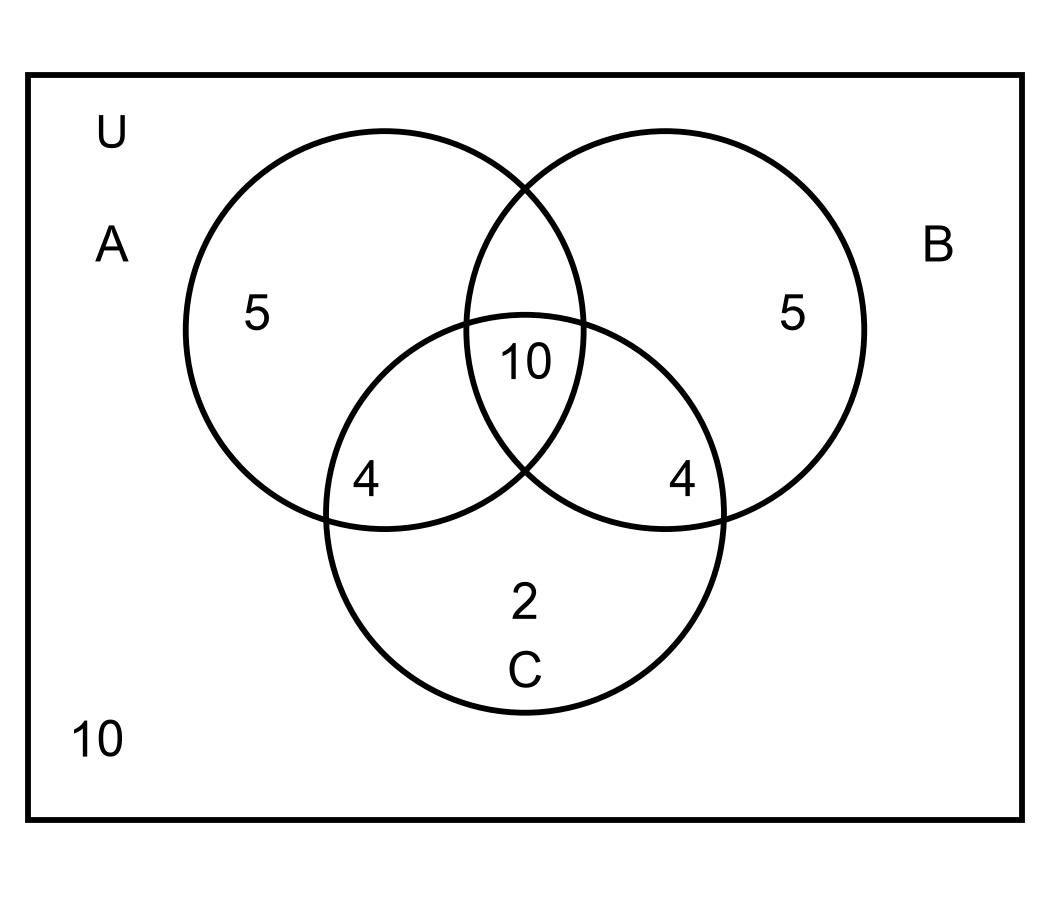
\includegraphics[width=0.38\textwidth]{figures/venn_50_ABC.png}
\end{center}
\step{所以单选物理、化学的人数至多 10 人.}
\step{所以至多选选择物理和化学这两门课程的学生人数至多 $10+10=20$ 人.}
\step{故选 C.}
\solend

\fi

\item 设 $k\geqslant 1,\,k\in\mathbb{N}$，已知集合 $M=\{1,2,3,4,5\}$，若集合 $N_1,N_2,\dots,N_k$ 是集合 $M$ 的 $k$ 个不同非空子集，且 $N_1\cup N_2\cup\dots\cup N_k\neq M$，则 $k$ 的最大值为\mbox{（\quad）.}

\keepwithprev
A. $15$\qquad B. $16$\qquad C. $31$\qquad D. $32$

\ans{A}

\ifanswer
\solbegin
\step{由 $N_1\cup N_2\cup\dots\cup N_k\neq M$ 得所有非空子集的并集缺少集合 $M$ 中至少一个元素.}
\step{假设缺少元素 1，则所有非空子集 $N_i$ 均不含元素 1，即 $N_i$ 是集合 $\{2,3,4,5\}$ 非空子集，集合 $\{2,3,4,5\}$ 的非空子集个数为 $2^4-1=15$，且这些子集 $N_i$ 的并集必不含 1，满足条件.}
\step{假设 $k\geqslant 16$，要满足所有非空子集的并集不等于集合 $M$，必须至少有一个集合 $M$ 中的元素不在任何一个子集中，否则并集就会等于 $M$.}
\step{设这个缺失的元素是 1，那么 $k$ 个非空集都不含元素 1，即每个子集都是集合 $\{2,3,4,5\}$ 的非空子集.}
\step{而集合 $\{2,3,4,5\}$ 只有 $2^4-1=15$ 个不同的非空子集，所以无法从中取出至少 16 个不同的非空子集.}
\step{因此假设不成立，$k$ 必须小于 16.}
\step{所以 $k$ 的最大值为 15，故选 A.}
\solend

\fi

% 注：原卷此题的差集记号是反斜杠 $A\setminus B$（本稿曾误作 $A\vee B$）；$C$ 的集合描述里原卷留了一条
%     待填横线“$x\in A\underline{\quad}B$”（选项按填入的符号分四种情形），本稿曾误作 $\vee\vee$。
%     2026-09-15 回原图核对时已按原卷改回。
\item 对于集合 $A$、$B$，定义 $A\setminus B=\{x\mid x\in A\text{ 且 }x\notin B\}$，则对于集合 $A=\{x\mid x=6n+5,\,n\in\mathbb{N}\}$，$B=\{y\mid y=3m+7,\,m\in\mathbb{N}\}$，$C=\{x\mid x\in A\underline{\hspace{4em}}B\text{ 且 }x<1000\}$，以下说法正确的是\mbox{（\quad）.}

\keepwithprev
A. 若在横线上填入“$\cap$”，则 $C$ 的真子集有 $2^{12}-1$ 个；

B. 若在横线上填入“$\cup$”，则 $C$ 中元素个数大于 250；

C. 若在横线上填入“$\setminus$”，则 $C$ 的非空真子集有 $2^{153}-2$ 个；

% 注：原卷选项 D 作“若在横线上填入“$\cup\complement_{\mathbb N}$”，则 $\complement_{\mathbb N}C$ 中元素个数为 13”；
%     本稿曾把 $\complement_{\mathbb N}$ 抄成 $\varnothing$、把 $\complement_{\mathbb N}C$ 抄成 $C\setminus C$，2026-09-15 回原图核对时已订正。
D. 若在横线上填入“$\cup\complement_{\mathbb{N}}$”，则 $\complement_{\mathbb{N}}C$ 中元素个数为 13.

\ans{B}

\ifanswer
\solbegin
\step{$x=6n+5=3(2n+1)+2$，$y=3m+7=3(m+2)+1$，集合 $A$、$B$ 无公共元素.}
\step{选项 A 中，集合 $C$ 为空集，没有真子集，$A$ 错；}
\step{选项 B 中，由 $6n+5<1000$ 得 $n<165\tfrac{5}{6}$，由 $3m+7<1000$ 得 $m<331$，因此 $C$ 中元素个数为 $166+331=497$，B 正确；}
\step{选项 C 中，$C$ 中元素个数为 166，非空真子集个数为 $2^{166}-2$，C 错；}
% 注：原卷此行作“$\complement_{\mathbb N}C=\complement_{\mathbb N}(A\cup\complement_{\mathbb N}B)
%     =\complement_{\mathbb N}A\cap\complement_{\mathbb N}(\complement_{\mathbb N}B)=\complement_{\mathbb N}A\cap B$，
%     而 $B\subseteq\complement_{\mathbb N}A$”；本稿曾把 $\complement_{\mathbb N}$ 抄成 $C\setminus$，同日已订正。
\step{选项 D 中，$\complement_{\mathbb{N}}C=\complement_{\mathbb{N}}(A\cup\complement_{\mathbb{N}}B)=\complement_{\mathbb{N}}A\cap\complement_{\mathbb{N}}(\complement_{\mathbb{N}}B)=\complement_{\mathbb{N}}A\cap B$，而 $B\subseteq\complement_{\mathbb{N}}A$.}
\step{因此其中元素个数为 331 个，D 错.}
\step{故选 B.}
\solend

\fi
\end{enumerate}

\bigsec{三、解答题}

\begin{enumerate}
\setcounter{enumi}{16}

\item 已知集合 $A=\{x\mid x<-1\text{ 或 }x>4\}$，$B=\{x\mid m+1\leqslant x\leqslant 2m+4\}$.
\begin{enumerate}[label=(\arabic*)]
\item 若 $m=2$，求 $A\cup B$ 和 $\left(\complement_{\R} A\right)\cap B$；
\item 若 $A\cap B=\varnothing$，求 $m$ 的取值范围.
\end{enumerate}

\ans{（1）$A\cup B=\{x\mid x<-1\text{ 或 }x\geqslant 3\}$，$\left(\complement_{\R} A\right)\cap B=\{x\mid 3\leqslant x\leqslant 4\}$；（2）$(-\infty,-3)\cup[-2,0]$}

\ifanswer
\solbegin
\stepm{(1)}{当 $m=2$ 时，集合 $B=\{x\mid 3\leqslant x\leqslant 8\}$.}
\step{又因为 $A=\{x\mid x<-1\text{ 或 }x>4\}$，则 $\complement_{\R}A=\{x\mid -1\leqslant x\leqslant 4\}$，所以 $A\cup B=\{x\mid x<-1\text{ 或 }x\geqslant 3\}$，$\left(\complement_{\R} A\right)\cap B=\{x\mid 3\leqslant x\leqslant 4\}$.}
\stepm{(2)}{因为 $A\cap B=\varnothing$，所以当 $B=\varnothing$ 时，$m+1>2m+4$，解得 $m<-3$ 满足题意；}
\step{当 $B\neq\varnothing$ 时，要满足题意，只需 $\begin{cases}m+1\leqslant 2m+4 \\ m+1\geqslant -1 \\ 2m+4\leqslant 4\end{cases}$，解得 $-2\leqslant m\leqslant 0$.}
\step{综上，实数 $m$ 的范围为 $m<-3$ 或 $-2\leqslant m\leqslant 0$，即 $(-\infty,-3)\cup[-2,0]$.}
\solend

\fi
\ansspace[6]
\item 设集合 $A=\{x\mid x^2+4x=0\}$，$B=\{x\mid x^2+2(a+1)x+a^2-1=0\}$.
\begin{enumerate}[label=(\arabic*)]
\item 写出集合 $A$ 的所有子集；
\item 若 $A\cap B=B$，求实数 $a$ 的取值范围.
\end{enumerate}

\ans{（1）$\{\varnothing,\{0\},\{-4\},\{0,-4\}\}$；（2）$a=1$ 或 $a\leqslant -1$}

\ifanswer
\solbegin
% 注：原卷此行印作“集合 $A$ 的所有子集为 $\varnothing,\{0\},\{-4\},\{0-4\}$”（末项漏逗号、且未加外层花括号）；
%     本稿按规范的列举写法给出，2026-09-15 回原图核对时加注。
\stepm{(1)}{由题意得 $A=\{0,-4\}$，集合 $A$ 的所有子集为 $\varnothing,\{0\},\{-4\},\{0,-4\}$.}
\stepm{(2)}{由 $A\cap B=B$ 得 $B\subseteq A$，所以 $B=\{0\}$ 或 $B=\{-4\}$ 或 $B=\{0,-4\}$ 或 $B=\varnothing$.}
\step{若 $B=\{0\}$ 时，$x^2+2(a+1)x+a^2-1=0$ 有两个相等的根 $0$，则 $\begin{cases}-2(a+1)=0 \\ a^2-1=-4\times(-4)\end{cases}$，解得 $a=-1$.}
\step{若 $B=\{-4\}$ 时，$x^2+2(a+1)x+a^2-1=0$ 有两个相等的根 $-4$，则 $\left\{\begin{matrix}-2(a+1)=-8 \\ a^2-1=-4\times(-4)\end{matrix}\right.$，$a$ 无解.}
\step{若 $B=\{0,-4\}$ 时，$x^2+2(a+1)x+a^2-1=0$ 有两个不相等的根 $0$ 和 $-4$，则 $\begin{cases}-2(a+1)=-4 \\ a^2-1=0\end{cases}$，解得 $a=1$.}
\step{当 $B=\varnothing$ 时，$x^2+2(a+1)x+a^2-1=0$ 无实数根，$\Delta=[2(a+1)]^2-4(a^2-1)=8a+8<0$，得 $a<-1$.}
\step{综上，$a=1$ 或 $a\leqslant -1$.}
\solend

\fi
\ansspace[6]
\item 已知集合 $A=\{x\mid x^2-5x+6=0\}$，$B=\{x\mid mx+1=0\}$，$C=\{x\in\mathbb{N}\mid \sqrt{x}\leqslant 1\}$，且 $A\cup B=A$.
\begin{enumerate}[label=(\arabic*)]
\item 求集合 $M=\{x\mid x\subseteq A\}$ 的真子集的个数；
\item 求实数 $m$ 的值组成的集合；
% 注：原卷本题的定义作“集合 $E=\{x\mid -x\in D,\,2-x^2\notin D\}$”；本稿曾把 $\notin$ 抄成 $\in$
%     （那样 $E=\varnothing$，与答案 $-5$ 冲突），2026-09-15 回原图核对时已订正。
\item 若集合 $D=A\cup C$，定义：集合 $E=\{x\mid -x\in D,\,2-x^2\notin D\}$，求集合 $E$ 中所有元素的和.
\end{enumerate}

\ans{（1）$15$；（2）$\left\{0,-\tfrac{1}{2},-\tfrac{1}{3}\right\}$；（3）$-5$}

\ifanswer
\solbegin
\stepm{(1)}{$A=\{x\mid x^2-5x+6=0\}=\{2,3\}$.}
\step{由 $M=\{x\mid x\subseteq A\}$ 得 $M$ 是 $A$ 的所有子集构成的集合，集合 $A$ 有 2 个元素，故 $A$ 的子集共 $2^2=4$ 个，即 $M$ 含 4 个元素，$M$ 的真子集个数为 $2^4-1=15$.}
\stepm{(2)}{由 (1) 得 $A=\{2,3\}$，集合 $B=\{x\mid mx+1=0\}$.}
\step{由 $A\cup B=A$ 得 $B\subseteq A$，分两种情况：① 当 $m=0$ 时，方程 $mx+1=0$ 无解，$B=\varnothing$，空集是任意集合的子集，符合条件；}
\stepm{②}{当 $m\neq 0$ 时，$B=\{-\tfrac{1}{m}\}$，由 $B\subseteq A$ 得 $-\tfrac{1}{m}=2$ 或 $-\tfrac{1}{m}=3$，解得 $m=-\tfrac{1}{2}$ 或 $m=-\tfrac{1}{3}$.}
\step{实数 $m$ 的取值集合为 $\left\{0,-\tfrac{1}{2},-\tfrac{1}{3}\right\}$.}
\stepm{(3)}{由 (1) 得 $A=\{2,3\}$.}
\step{由 $x\in\mathbb{N}$ 且 $\sqrt{x}\leqslant 1$，得 $x=0$ 或 $x=1$，故 $C=\{0,1\}$.}
\step{所以 $D=A\cup C=\{0,1,2,3\}$.}
\step{由 $-x\in D$ 得 $x$ 的候选值为 $0,-1,-2,-3$.}
\step{由于集合 $E=\{x\mid -x\in D,\,2-x^2\in D\}$，当 $x=0$ 时，$2-x^2=2\in D$，不符合题意；}
\step{当 $x=-1$ 时，$2-x^2=1\in D$，不符合题意；}
\step{当 $x=-2$ 时，$2-x^2=-2\notin D$，符合题意；}
\step{当 $x=-3$ 时，$2-x^2=-7\notin D$，符合题意.}
\step{故 $E=\{-2,-3\}$，所有元素的和为 $-2+(-3)=-5$.}
\solend

\fi
\ansspace[8]
\item 设集合 $M$ 是至少含有两个元素的数集，若 $M$ 中存在两个元素 $x$、$y$ 满足它们的积 $xy\in M$，则称 $M$ 为可积数集.
\begin{enumerate}[label=(\arabic*)]
\item 设集合 $A=\{2,3,5\}$，试判断 $A$ 是否为可积数集？并说明理由；
\item 设集合 $B=\{2,3,4,a\}$，若 $B$ 为可积数集，求实数 $a$ 的取值集合；
\item 设集合 $D=\{x\mid t<x<t+2\}$，若 $D$ 不是可积数集，求实数 $t$ 的取值范围.
\end{enumerate}

% 注：原卷本题【答案】与文末解析的结论都含 $\frac{3}{4}$；本稿曾漏掉 $\frac{3}{4}$
%     （与本稿自己的解析结论不一致），2026-09-15 回原图核对时已订正。
\ans{（1）否；（2）$\left\{0,\tfrac{1}{2},\tfrac{2}{3},\tfrac{3}{4},1,\tfrac{4}{3},\tfrac{3}{2},6,8,12\right\}$；（3）$t\in(-\infty,-2]\cup[2,+\infty)$}

\ifanswer
\solbegin
\stepm{(1)}{因为 $2\times 3=6\notin A$，$2\times 5=10\notin A$，$3\times 5=15\notin A$，所以 $A$ 中任意两个元素的积都不是 $A$ 中的元素，即 $A$ 不是可积数集.}
\stepm{(2)}{若 $B=\{2,3,4,a\}$ 为可积数集，则 $2\times 3=6\in B$，或 $2\times 4=8\in B$ 或 $3\times 4=12\in B$ 或 $2a\in B$ 或 $3a\in B$ 或 $4a\in B$.}
\step{若 $6\in B$，则 $a=6$；}
\step{若 $8\in B$，则 $a=8$；}
\step{若 $12\in B$，则 $a=12$；}
\step{若 $2a\in B$，则 $2a=2$ 或 $2a=3$ 或 $2a=4$ 或 $2a=a$，解得 $a=1$ 或 $a=\tfrac{3}{2}$ 或 $a=2$（舍）或 $a=0$；}
\step{若 $3a\in B$，则 $3a=2$ 或 $3a=3$ 或 $3a=4$ 或 $3a=a$，解得 $a=\tfrac{2}{3}$ 或 $a=1$ 或 $a=\tfrac{4}{3}$ 或 $a=0$；}
\step{若 $4a\in B$，则 $4a=2$ 或 $4a=3$ 或 $4a=4$ 或 $4a=a$，解得 $a=\tfrac{1}{2}$ 或 $a=\tfrac{3}{4}$ 或 $a=1$ 或 $a=0$.}
\step{综上，实数 $a$ 的取值集合为 $\left\{0,\tfrac{1}{2},\tfrac{2}{3},\tfrac{3}{4},1,\tfrac{4}{3},\tfrac{3}{2},6,8,12\right\}$.}
\stepm{(3)}{若 $D=\{x\mid t<x<t+2\}$ 不是可积数集，则 $\forall x,y\in(t,t+2)$，$xy\notin(t,t+2)$.}
\step{当 $t+2\leqslant 0$，即 $t\leqslant -2$ 时，$0\leqslant(t+2)^2<xy<t^2$，此时 $xy\notin D$，满足题意；}
\step{当 $t\geqslant 0$ 时，$0\leqslant t^2<xy<(t+2)^2$，因为 $(t+2)^2>t$，所以若 $xy\notin D$，则 $t^2\geqslant t+2$，即 $t^2-t-2\geqslant 0$，解得 $t\geqslant 2$ 或 $t\leqslant -1$，此时 $t\geqslant 2$ 满足题意；}
% 注：原卷此句作“当 $t<0<t+2$，即 $-2<t<0$ 时，$\exists x=0$，$xy=0\in D$，不满足题意，舍去”；
%     本稿曾把 $\in D$ 抄成 $\notin D$（$-2<t<0$ 时 $0\in(t,t+2)$，确有 $0\in D$），同日已订正。
\step{当 $t<0<t+2$，即 $-2<t<0$ 时，$\exists x=0$，$xy=0\in D$，不满足题意，舍去.}
\step{综上，所求实数 $t$ 的取值范围为 $t\geqslant 2$ 或 $t\leqslant -2$，故 $t\in(-\infty,-2]\cup[2,+\infty)$.}
\solend

\fi
\ansspace[8]
\ansneed{7cm}
\item 已知集合 $A$ 为非空数集，定义：$S=\{x\mid x=a+b,\,a,b\in A\}$，$T=\{x\mid x=|a-b|,a,b\in A\}$（实数 $a$、$b$ 可以相同）.
\begin{enumerate}[label=(\arabic*)]
\item 若集合 $A=\{2,5\}$，直接写出集合 $S$、$T$；
\item 若集合 $A=\{x_1,x_2,x_3,x_4\}$，$x_1<x_2<x_3<x_4$，且 $T=A$，求证：$x_1+x_4=x_3+x_2$；
\item 若集合 $A\subseteq\{x\mid 0\leqslant x\leqslant 2025,\,x\in\mathbb{N}\}$，$S\cap T=\varnothing$，记 $|A|$ 为集合 $A$ 中的元素个数，求 $|A|$ 的最大值.
\end{enumerate}

\ans{（1）$S=\{4,7,10\}$，$T=\{0,3\}$；（2）略；（3）$1350$}

\ifanswer
\solbegin
\stepm{(1)}{$S=\{4,7,10\}$，$T=\{0,3\}$.}
\stepm{(2)}{由集合 $A=\{x_1,x_2,x_3,x_4\}$，$x_1<x_2<x_3<x_4$，则 $T$ 集合的元素在 $0,x_2-x_1,x_3-x_1,x_4-x_1,x_3-x_2,x_4-x_2,x_4-x_3$ 中，且 $0<x_2-x_1<x_3-x_1<x_4-x_1$，$x_3-x_2<x_4-x_2<x_4-x_3$，因为 $A=T$，所以 $A$ 中最大元素 $x_4$ 必在 $T$ 中，而 $x_4-x_1$ 为 7 个元素中的最大者.}
\step{故 $x_4=x_4-x_1$，即 $x_1=0$.}
\step{故 $A=\{0,x_2,x_3,x_4\}$.}
\step{则 $x_3-x_2$、$x_4-x_2$、$x_4-x_3$ 与 $x_2$、$x_3$、$x_4$ 重复.}
\step{而 $0<x_3-x_2<x_3$，故 $x_3-x_2=x_2$，即 $x_3=2x_2$.}
% 注：原卷此句作“而 $0<x_4-x_3<x_4$，故 $x_4-x_3=x_2$ 或 $x_4-x_3=x_3$”；本稿曾把上界写成 $x_3$
%     （那样排除不了 $x_4-x_3=x_3$，与后半句自相矛盾），2026-09-15 回原图核对时已订正。
\step{而 $0<x_4-x_3<x_4$，故 $x_4-x_3=x_2$ 或 $x_4-x_3=x_3$.}
\step{若 $x_4=2x_3=4x_2$，则 $A=\{0,x_2,2x_2,4x_2\}$，$4x_2-x_2=3x_2\notin T$，与题设矛盾.}
\step{故 $x_4-x_3=x_2$，又因为 $x_1=0$，所以 $x_4+x_1=x_3+x_2$.}
% 注：原卷此行作“则 $2a_1<a_1+a_2<a_1+a_3<\cdots<a_1+a_k<a_2+a_k<a_3+a_k<\cdots<a_{k-1}+a_k<2a_k$，
%     所以 $|S|\geqslant 2k-1$，$a_1-a_1<a_2-a_1<a_3-a_1<\cdots<a_k-a_1$，所以 $|T|\geqslant k$”；
%     本稿曾把这个不等式链抄乱（作 $\cdots<a_1+a_k<a_2+a_3<a_k+a_k\leqslant 2a_k$）且把首项写成 $a_i-a_1$，
%     2026-09-15 回原图核对时已订正。
\stepm{(3)}{设 $A=\{a_1,a_2,\dots,a_k\}$ 满足题意，其中 $a_1<a_2<\dots<a_k$，则 $2a_1<a_1+a_2<a_1+a_3<\dots<a_1+a_k<a_2+a_k<a_3+a_k<\dots<a_{k-1}+a_k<2a_k$，所以 $|S|\geqslant 2k-1$，$a_1-a_1<a_2-a_1<a_3-a_1<\dots<a_k-a_1$，所以 $|T|\geqslant k$.}
\step{因为 $S\cap T=\varnothing$，由容斥原理得 $|S\cup T|=|S|+|T|\geqslant 3k-1$.}
\step{$S\cup T$ 中最小的元素为 0，最大的元素为 $2a_k$，$|S\cup T|\leqslant 2a_k+1$，所以 $3k-1\leqslant 2a_k+1\leqslant 2\times 2025+1\,(k\geqslant 1,k\in\mathbb{N})$，即 $3k-1\leqslant 4051$，解得 $k\leqslant 1350\tfrac{2}{3}$.}
\step{实际上 $A=\{676,677,678,\dots,2025\}$ 时满足题意，证明如下：设 $A=\{m,m+1,m+2,\dots,2025\}$，$m\in\mathbb{N}$.}
\step{则 $S=\{2m,2m+1,2m+2,\dots,4050\}$，$T=\{0,1,2,\dots,2025-m\}$.}
\step{由题意得 $2025-m<2m$，即 $m>675$.}
\step{所以 $A=\{676,677,678,\dots,2025\}$ 时满足题意，此时集合 $A$ 中的元素的个数最多.}
\step{综上所述，集合 $A$ 中元素的个数的最大值是 1350.}
\solend

\fi
\ansspace*[10]
\end{enumerate}

\end{document}"
% 紧凑版：xelatex "\def\iscompact{1}% 高一07_交附闵行_周练1.tex —— 高一上数学“2026-2027 年交附闵行高一上周练 1”（试卷版/答案版）
% 试卷版：xelatex 高一07_交附闵行_周练1.tex
% 答案版：xelatex "\def\isanswer{1}\input{高一07_交附闵行_周练1.tex}"
% 紧凑版：xelatex "\def\iscompact{1}\input{高一07_交附闵行_周练1.tex}"
%
% 原始材料是微信公众号图文（“魔都数学加油站”，作者署名“破晓”），正文为 11 张 PNG 页
% （1080×1527）；卷面上的粉色斜水印“魔都数学加油站”属水印，未录入。原文本身就是一份
% **讲评版**——题下直接印出【答案】或【解析】，本稿把这些答案与解析移到答案版，试卷版即
% 一张干净的空卷。
%
% 与原卷的排版差异（均已在 README“说明”中交代）：
%   ① 原文自**第 3 题**起（第 1、2 题未在该文发布），源码里以 \setcounter{enumi}{2} 起编；
%   ② 原卷本就印有分节标题“一、填空题”“二、选择题”“三、解答题”（已在原图上逐页放大
%      核对过），本稿照原卷分节，只把标题改排成全稿统一的“大节标题”样式；
%   ③ 原卷的实数集、整数集符号作正体 $R$（第 7 题）、$Z$（第 11 题），本稿按全稿惯例统一
%      写作 $\R$、$\Z$；
%   ④ 第 14 题【解析】里的 Venn 图取自原卷截图（`figures/venn_50_ABC.png`，4× LANCZOS
%      放大），未用 TikZ 重绘.

\documentclass[a4paper,11pt]{article}
\usepackage{common}

\begin{document}

\examtitlest{2026--2027 学年度交附闵行高一上周练 1}{集合与常用逻辑用语}

\bigsec{一、填空题}

\begin{enumerate}
\setcounter{enumi}{2}

\item 已知集合 $A=\{2,14,x^2+5\}$，$B=\{2,2x\}$，若 $A\cap B=B$，则实数 $x=$ \blankline[2em].

\ans{$7$}

\ifanswer
\solbegin
\step{因为 $A\cap B=B$，所以 $B\subseteq A$，所以 $2x=14$ 或 $x^2+5=2x$.}
\step{$2x=14$ 时，$x=7$，此时 $A=\{2,14,54\}$，$B=\{2,14\}$ 满足题意；}
\step{$x^2+5=2x$ 时，$(x-1)^2+4=0$，无解.}
\step{所以 $x=7$.}
\solend

\fi
\item 设集合 $A=\{y\mid y=x^2-1\}$，$B=\{(x,y)\mid y=x\}$，则 $A\cap B=$ \blankline[2em].

\ans{$\varnothing$}

\item 若集合 $\{0,-1,2a\}=\{a-1,-|a|,a+1\}$，实数 $a$ 的值为 \blankline[2em].

\ans{$\pm 1$}

\ifanswer
\solbegin
\step{令 $A=\{0,-1,2a\}$，$B=\{a-1,-|a|,a+1\}$，因为 $\{0,-1,2a\}=\{a-1,-|a|,a+1\}$，若 $a-1=0$，则 $a=1$，则 $A=\{0,-1,2\}$，$B=\{0,-1,2\}$，满足要求；}
\step{若 $-|a|=0$，则 $a=0$，则 $A=\{0,-1,0\}$，不满足集合元素的互异性；}
\step{若 $a+1=0$，则 $a=-1$，则 $A=\{0,-1,-2\}$，$B=\{0,-1,-2\}$，满足要求.}
\step{故实数 $a$ 的值为 $\pm 1$.}
\solend

\fi
\item 已知全集 $U=(-4,3]$，$A=\{x\in U\mid x^2+2x-8=0\}$，$B=\{x\in U\mid -3<1-2x\leqslant 5\}$，则 $\left(\complement_U B\right)\cap A=$ \blankline[2em].

\ans{$\{2\}$}

\item 已知集合 $A=\{x\mid 1-a\leqslant x\leqslant 1+a,\,a\in\R\}$ 中只有一个整数元素，则实数 $a$ 的取值范围为 \blankline[2em].

\ans{$[0,1)$}

\ifanswer
\solbegin
\step{集合 $A=\{x\mid 1-a\leqslant x\leqslant 1+a,\,a\in\R\}$ 中只有一个整数元素，则 $A\neq\varnothing,\,1-a\leqslant 1+a$，即 $a\geqslant 0$，此时 $1\in A$，故 $\begin{cases}1+a<2 \\ 1-a>0\end{cases}$，解得 $a<1$.}
\step{故 $a\in[0,1)$.}
\solend

\fi
\item 已知全集 $U=\{x\in\mathbb{N}\mid x\leqslant 9\}$，$A\cap B=\{3\}$，$\overline{A}\cap B=\{4,6,8\}$，$A\cap\overline{B}=\{1,5\}$，则 $\overline{A}=$ \blankline[2em].

\ans{$\{0,2,4,6,7,8,9\}$}

\ifanswer
\solbegin
\step{由题意得 $U=\{x\in\mathbb{N}\mid x\leqslant 9\}=\{0,1,2,3,4,5,6,7,8,9\}$，$A\cap B=\{3\}$ 得 $A$、$B$ 中含有元素 $3$；}
\step{$\overline{A}\cap B=\{4,6,8\}$ 得 $B$ 中含有 $4$、$6$、$8$，集合 $A$ 中不含 $4$、$6$、$8$；}
\step{$A\cap\overline{B}=\{1,5\}$ 得 $A$ 含有 $1$、$5$，集合 $B$ 不含 $1$、$5$.}
\step{对于 $0$，假设集合 $A$ 中含有 $0$，由 $A\cap B=\{3\}$ 得 $B$ 不含 $0$，则 $A\cap\overline{B}$ 必含元素 $0$，与 $A\cap\overline{B}=\{1,5\}$ 矛盾.}
\step{同理可得集合 $A$ 中不含元素 $2$、$7$、$9$.}
\step{综上所述，$A=\{1,3,5\}$.}
\step{故 $\overline{A}=\{0,2,4,6,7,8,9\}$.}
\solend

\fi
\item 已知一个有四个数字元素的集合 $S$，$S$ 的所有子集的元素和（空集的元素和认为是 0）的总和为 16208，则 $S$ 的元素之和等于 \blankline[2em].

\ans{$2026$}

\ifanswer
\solbegin
\step{设 $S=\{a_1,a_2,a_3,a_4\}$，$S$ 的每个元素在所有子集中均出现 $2^3$ 次，故 $(a_1+a_2+a_3+a_4)\cdot 2^3=16208$，所以 $a_1+a_2+a_3+a_4=2026$，故 $S$ 的元素之和等于 2026.}
\solend

\fi
\item 已知集合 $M=\{x\in\mathbb{N}\mid 1\leqslant x\leqslant 12\}$，集合 $A_1$、$A_2$、$A_3$ 满足：① 每个集合都恰有 4 个元素；② $A_1\cup A_2\cup A_3=M$. 集合 $A_i\,(i=1,2,3)$ 中元素的最大值与最小值之和称为集合 $A_i$ 的特征数，记为 $X_i\,(i=1,2,3)$，则 $X_1+X_2+X_3$ 的最大值与最小值的积为 \blankline[2em].

\ans{$1485$}

\ifanswer
\solbegin
\step{集合 $M=\{x\in\mathbb{N}\mid 1\leqslant x\leqslant 12\}$ 中最小值为 1，最大值为 12.}
% 注：原卷此处印作“则 $A_1=13$”（原卷笔误，按上下文应为 $X_1=13$），本稿按 $X_1$ 规范，2026-09-15 回原图核对时加注。
\stepm{①}{若使 $X_1+X_2+X_3$ 取得最大值，不妨设 $A_1=\{1,2,3,12\}$，则 $X_1=13$，则剩余的数中最小值是 4，最大值是 11，令 $A_2=\{4,5,6,11\}$，则 $X_2=15$，则 $A_3=\{7,8,9,10\}$，$X_3=17$，则 $X_1+X_2+X_3$ 的最大值为 $13+15+17=45$；}
\stepm{②}{若使 $X_1+X_2+X_3$ 取得最小值，则 $A_1=\{1,4,5,6\}$，则 $X_1=7$，令 $A_2=\{2,7,8,9\}$，则 $X_2=11$，则 $A_3=\{3,10,11,12\}$，$X_3=15$，则此时 $X_1+X_2+X_3$ 的最小值为 $7+11+15=33$.}
\step{故 $X_1+X_2+X_3$ 的最大值与最小值的积为 $45\times 33=1485$.}
\solend

\fi
\item 对于集合 $M=\{a\mid a=x^2-y^2,\,x\in\Z,\,y\in\Z\}$，给出如下三个结论：

① 如果 $P=\{b\mid b=2n+1,\,n\in\Z\}$，那么 $P\subseteq M$；

% 注：原卷此条作“如果 $c=4n+2$，$n\in\Z$，那么 $c\notin M$”；本稿曾把 $\notin$ 抄成 $\in$
%     （那样②为假，与本卷答案 ①②③ 冲突），2026-09-15 回原图核对时已订正。
② 如果 $c=4n+2$，$n\in\Z$，那么 $c\notin M$；

③ 如果 $a_1\in M$，$a_2\in M$，那么 $a_1a_2\in M$. 其中正确结论的序号是 \blankline[2em].

\ans{①②③}

\ifanswer
\solbegin
\stepm{①}{由已知 $b=2n+1,\,n\in\Z$，则恒有 $2n+1=(n+1)^2-n^2,\,n\in\Z$，所以 $2n+1\in M$，所以 $P\subseteq M$，所以①正确；}
\stepm{②}{元素 $c=4n+2,\,n\in\Z$，若 $4n+2\in M$，则存在 $x$、$y\in\Z$ 使得 $x^2-y^2=4n+2$，所以 $4n+2=(x+y)(x-y)$，则 $x+y$ 与 $x-y$ 同奇或同偶.}
\step{若 $x+y$ 与 $x-y$ 都是奇数，则 $(x+y)(x-y)$ 为奇数，而 $4n+2$ 是偶数；}
\step{若 $x+y$ 和 $x-y$ 都是偶数，则 $(x+y)(x-y)$ 能被 4 整除，而 $4n+2$ 不能被 4 整除.}
\step{所以 $4n+2\notin M$，即 $c\notin M$，故②正确；}
\stepm{③}{因为 $a_1$、$a_2\in M$，则 $a_1a_2$ 还是整数，所以 $a_1a_2\in M$，故③正确.}
\step{故正确的是①②③.}
\solend

\fi
\item 用 $C(A)$ 表示非空集合 $A$ 中的元素的个数，定义 $A*B=|C(A)-C(B)|$，若 $A=\{x\mid x^2-2024x-2025=0\}$，$B=\{x\mid (2x^2+ax)(x^2+2ax+6)=0\}$，若 $A*B=1$，则 $a$ 的所有可能取值构成集合 $M$，则 $C(M)=$ \blankline[2em].

\ans{$5$}

\ifanswer
\solbegin
\step{$x^2-2024x-2025=0$ 得 $x=2025$ 或 $x=-1$，即 $C(A)=2$，因为 $A*B=|C(A)-C(B)|=1$，所以 $C(B)=3$ 或 $C(B)=1$.}
\step{方程 $(2x^2+ax)(x^2+2ax+6)=0$ 化为 $x(2x+a)(x^2+2ax+6)=0$.}
\step{当 $a=0$ 时，方程化为 $2x^3(x^2+6)=0$，解得 $x=0$，所以 $B=\{0\}$，$C(B)=1$，符合题意.}
\step{当 $a\neq 0$ 时，方程化为 $x=0$ 或 $x=-\tfrac{a}{2}$ 或 $x^2+2ax+6=0$.}
\step{因为 $0\neq -\tfrac{a}{2}$，$C(B)\neq 1$，故只有 $C(B)=3$.}
\step{故 $x^2+2ax+6=0$ 有两个相等的非零实数根，所以 $\Delta=4a^2-4\times 6=0$，解得 $a=\pm\sqrt{6}$，符合题意.}
\step{当 $x^2+2ax+6=0$ 有两个不相等实根，设 $x_1$、$x_2$，若 $x_1=-\tfrac{a}{2}$，由韦达定理得 $\begin{cases}x_1+x_2=-2a \\ x_1x_2=6\end{cases}$，% 注：原卷作“得 $x_2=-\frac{3a}{2}$”（由 $x_1+x_2=-2a$、$x_1=-\frac{a}{2}$ 得 $x_2=-\frac{3a}{2}$）；
%     本稿曾漏掉负号，2026-09-15 回原图核对时已订正。
得 $x_2=-\tfrac{3a}{2}$，$-\tfrac{a}{2}\cdot(-\tfrac{3a}{2})=\tfrac{3a^2}{4}=6$，解得 $a=\pm 2\sqrt{2}$，符合题意.}
\step{综上所述，$M=\{0,\sqrt{6},-\sqrt{6},2\sqrt{2},-2\sqrt{2}\}$，所以 $C(M)=5$.}
\solend

\fi
\end{enumerate}

\bigsec{二、选择题}

\begin{enumerate}
\setcounter{enumi}{12}

\item 已知集合 $A=\{1,2,3,4,5\}$，$B=\{x\mid \tfrac{x-1}{2}\in\Z,\,x\in A\}$，则集合 $B$ 的真子集个数为\mbox{（\quad）.}

\keepwithprev
A. $3$\qquad B. $5$\qquad C. $7$\qquad D. $15$

\ans{C}

\ifanswer
\solbegin
\step{已知集合 $A=\{1,2,3,4,5\}$，$B=\{x\mid\tfrac{x-1}{2}\in\Z,\,x\in A\}$.}
\step{因为 $\tfrac{x-1}{2}\in\Z$，所以 $x$ 为奇数，所以 $B=\{1,3,5\}$.}
\step{所以集合 $B$ 中有 3 个元素，所以集合 $B$ 的真子集个数为 $2^3-1=7$.}
\step{故选 C.}
\solend

\fi

\item 高一二班共有学生 50 人，每名学生要从物理、化学、生物、历史、地理、政治这六门课程中选择三门课程进行学习. 已知选择物理、化学、生物的学生各有至少 20 人，这三门课程都不选的有 10 人，这三门课程都选的有 10 人，在这三门课程中选择任意两门课程的都至少有 14 人，物理、化学只选一科的学生都至少 5 人，那么选择物理和化学这两门课程的学生人数至多\mbox{（\quad）.}

\keepwithprev
A. $18$\qquad B. $19$\qquad C. $20$\qquad D. $21$

\ans{C}

\ifanswer
\solbegin
\step{可以把学生 50 人看作一个集合 $U$，选择物理的人数组成集合 $A$，选择化学的人数组成集合 $B$，选择生物的人数组成集合 $C$.}
\step{要使选择物理和化学这两门课程的学生人数最多，除这三门课程都不选的有 10 人，这三门课程都选的有 10 人，则其他科选择人数均为最少，因为物理、化学只选一科的学生都至少 5 人，即得到单选物理的最少 5 人，单选化学的最少 5 人.}
\step{因为在这三门课程中选择任意两门课程的都至少有 14 人，单选化学、生物的最少 4 人，单选物理、生物的最少 4 人.}
\step{因为选择物理、化学、生物的学生各有至少 20 人，所以单选生物的最少 2 人.}
\step{以上人数最少 30 人，可作出如图所示的韦恩图：}
% 注：原卷此处印有一张韦恩图（三个圆 $A$、$B$、$C$，$A$ 独有 5、$B$ 独有 5、三集合公共 10、
%     $A\cap C$ 独有 4、$B\cap C$ 独有 4、$C$ 独有 2、三集合之外 10）；本稿此前漏排此图而正文仍作
%     “如图”，2026-09-15 回原图核对时按原卷截图补入（见 figures/venn_50_ABC.png）。
\begin{center}
% 插图取自原卷截图（裁去截图残影后 4× LANCZOS 放大），不用 TikZ 手绘
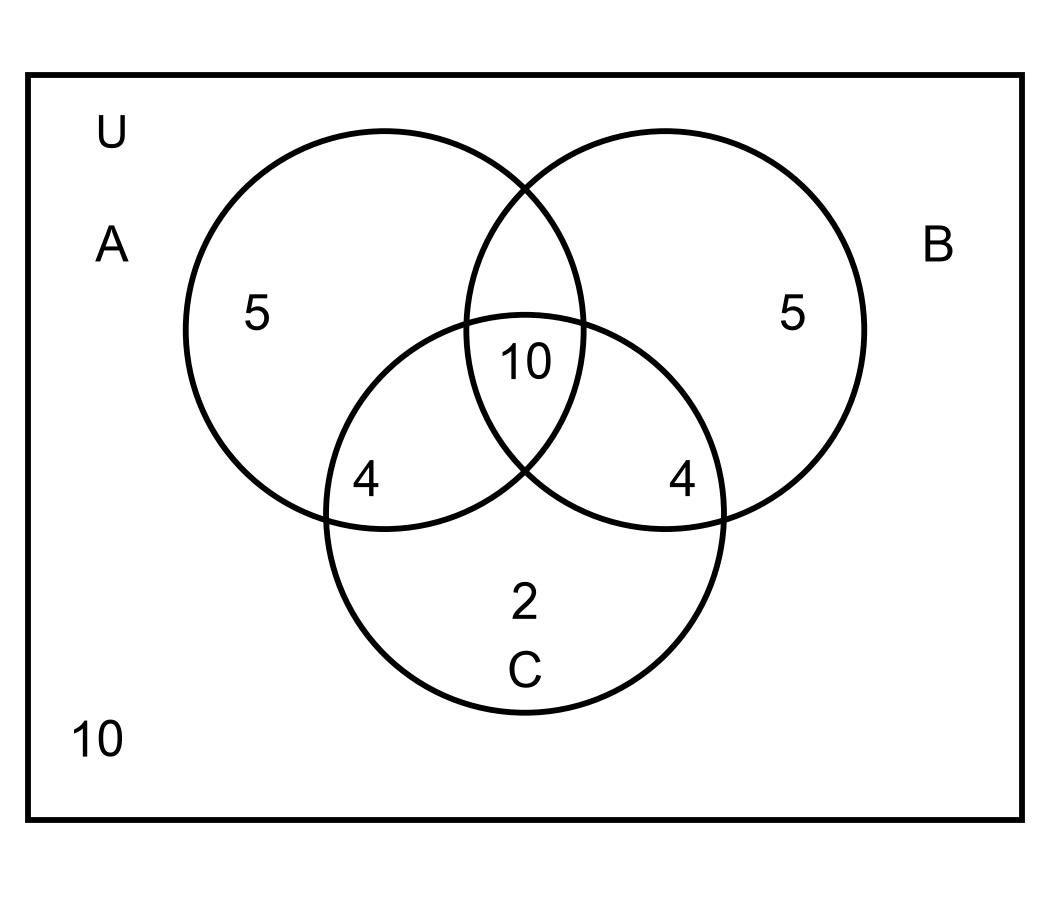
\includegraphics[width=0.38\textwidth]{figures/venn_50_ABC.png}
\end{center}
\step{所以单选物理、化学的人数至多 10 人.}
\step{所以至多选选择物理和化学这两门课程的学生人数至多 $10+10=20$ 人.}
\step{故选 C.}
\solend

\fi

\item 设 $k\geqslant 1,\,k\in\mathbb{N}$，已知集合 $M=\{1,2,3,4,5\}$，若集合 $N_1,N_2,\dots,N_k$ 是集合 $M$ 的 $k$ 个不同非空子集，且 $N_1\cup N_2\cup\dots\cup N_k\neq M$，则 $k$ 的最大值为\mbox{（\quad）.}

\keepwithprev
A. $15$\qquad B. $16$\qquad C. $31$\qquad D. $32$

\ans{A}

\ifanswer
\solbegin
\step{由 $N_1\cup N_2\cup\dots\cup N_k\neq M$ 得所有非空子集的并集缺少集合 $M$ 中至少一个元素.}
\step{假设缺少元素 1，则所有非空子集 $N_i$ 均不含元素 1，即 $N_i$ 是集合 $\{2,3,4,5\}$ 非空子集，集合 $\{2,3,4,5\}$ 的非空子集个数为 $2^4-1=15$，且这些子集 $N_i$ 的并集必不含 1，满足条件.}
\step{假设 $k\geqslant 16$，要满足所有非空子集的并集不等于集合 $M$，必须至少有一个集合 $M$ 中的元素不在任何一个子集中，否则并集就会等于 $M$.}
\step{设这个缺失的元素是 1，那么 $k$ 个非空集都不含元素 1，即每个子集都是集合 $\{2,3,4,5\}$ 的非空子集.}
\step{而集合 $\{2,3,4,5\}$ 只有 $2^4-1=15$ 个不同的非空子集，所以无法从中取出至少 16 个不同的非空子集.}
\step{因此假设不成立，$k$ 必须小于 16.}
\step{所以 $k$ 的最大值为 15，故选 A.}
\solend

\fi

% 注：原卷此题的差集记号是反斜杠 $A\setminus B$（本稿曾误作 $A\vee B$）；$C$ 的集合描述里原卷留了一条
%     待填横线“$x\in A\underline{\quad}B$”（选项按填入的符号分四种情形），本稿曾误作 $\vee\vee$。
%     2026-09-15 回原图核对时已按原卷改回。
\item 对于集合 $A$、$B$，定义 $A\setminus B=\{x\mid x\in A\text{ 且 }x\notin B\}$，则对于集合 $A=\{x\mid x=6n+5,\,n\in\mathbb{N}\}$，$B=\{y\mid y=3m+7,\,m\in\mathbb{N}\}$，$C=\{x\mid x\in A\underline{\hspace{4em}}B\text{ 且 }x<1000\}$，以下说法正确的是\mbox{（\quad）.}

\keepwithprev
A. 若在横线上填入“$\cap$”，则 $C$ 的真子集有 $2^{12}-1$ 个；

B. 若在横线上填入“$\cup$”，则 $C$ 中元素个数大于 250；

C. 若在横线上填入“$\setminus$”，则 $C$ 的非空真子集有 $2^{153}-2$ 个；

% 注：原卷选项 D 作“若在横线上填入“$\cup\complement_{\mathbb N}$”，则 $\complement_{\mathbb N}C$ 中元素个数为 13”；
%     本稿曾把 $\complement_{\mathbb N}$ 抄成 $\varnothing$、把 $\complement_{\mathbb N}C$ 抄成 $C\setminus C$，2026-09-15 回原图核对时已订正。
D. 若在横线上填入“$\cup\complement_{\mathbb{N}}$”，则 $\complement_{\mathbb{N}}C$ 中元素个数为 13.

\ans{B}

\ifanswer
\solbegin
\step{$x=6n+5=3(2n+1)+2$，$y=3m+7=3(m+2)+1$，集合 $A$、$B$ 无公共元素.}
\step{选项 A 中，集合 $C$ 为空集，没有真子集，$A$ 错；}
\step{选项 B 中，由 $6n+5<1000$ 得 $n<165\tfrac{5}{6}$，由 $3m+7<1000$ 得 $m<331$，因此 $C$ 中元素个数为 $166+331=497$，B 正确；}
\step{选项 C 中，$C$ 中元素个数为 166，非空真子集个数为 $2^{166}-2$，C 错；}
% 注：原卷此行作“$\complement_{\mathbb N}C=\complement_{\mathbb N}(A\cup\complement_{\mathbb N}B)
%     =\complement_{\mathbb N}A\cap\complement_{\mathbb N}(\complement_{\mathbb N}B)=\complement_{\mathbb N}A\cap B$，
%     而 $B\subseteq\complement_{\mathbb N}A$”；本稿曾把 $\complement_{\mathbb N}$ 抄成 $C\setminus$，同日已订正。
\step{选项 D 中，$\complement_{\mathbb{N}}C=\complement_{\mathbb{N}}(A\cup\complement_{\mathbb{N}}B)=\complement_{\mathbb{N}}A\cap\complement_{\mathbb{N}}(\complement_{\mathbb{N}}B)=\complement_{\mathbb{N}}A\cap B$，而 $B\subseteq\complement_{\mathbb{N}}A$.}
\step{因此其中元素个数为 331 个，D 错.}
\step{故选 B.}
\solend

\fi
\end{enumerate}

\bigsec{三、解答题}

\begin{enumerate}
\setcounter{enumi}{16}

\item 已知集合 $A=\{x\mid x<-1\text{ 或 }x>4\}$，$B=\{x\mid m+1\leqslant x\leqslant 2m+4\}$.
\begin{enumerate}[label=(\arabic*)]
\item 若 $m=2$，求 $A\cup B$ 和 $\left(\complement_{\R} A\right)\cap B$；
\item 若 $A\cap B=\varnothing$，求 $m$ 的取值范围.
\end{enumerate}

\ans{（1）$A\cup B=\{x\mid x<-1\text{ 或 }x\geqslant 3\}$，$\left(\complement_{\R} A\right)\cap B=\{x\mid 3\leqslant x\leqslant 4\}$；（2）$(-\infty,-3)\cup[-2,0]$}

\ifanswer
\solbegin
\stepm{(1)}{当 $m=2$ 时，集合 $B=\{x\mid 3\leqslant x\leqslant 8\}$.}
\step{又因为 $A=\{x\mid x<-1\text{ 或 }x>4\}$，则 $\complement_{\R}A=\{x\mid -1\leqslant x\leqslant 4\}$，所以 $A\cup B=\{x\mid x<-1\text{ 或 }x\geqslant 3\}$，$\left(\complement_{\R} A\right)\cap B=\{x\mid 3\leqslant x\leqslant 4\}$.}
\stepm{(2)}{因为 $A\cap B=\varnothing$，所以当 $B=\varnothing$ 时，$m+1>2m+4$，解得 $m<-3$ 满足题意；}
\step{当 $B\neq\varnothing$ 时，要满足题意，只需 $\begin{cases}m+1\leqslant 2m+4 \\ m+1\geqslant -1 \\ 2m+4\leqslant 4\end{cases}$，解得 $-2\leqslant m\leqslant 0$.}
\step{综上，实数 $m$ 的范围为 $m<-3$ 或 $-2\leqslant m\leqslant 0$，即 $(-\infty,-3)\cup[-2,0]$.}
\solend

\fi
\ansspace[6]
\item 设集合 $A=\{x\mid x^2+4x=0\}$，$B=\{x\mid x^2+2(a+1)x+a^2-1=0\}$.
\begin{enumerate}[label=(\arabic*)]
\item 写出集合 $A$ 的所有子集；
\item 若 $A\cap B=B$，求实数 $a$ 的取值范围.
\end{enumerate}

\ans{（1）$\{\varnothing,\{0\},\{-4\},\{0,-4\}\}$；（2）$a=1$ 或 $a\leqslant -1$}

\ifanswer
\solbegin
% 注：原卷此行印作“集合 $A$ 的所有子集为 $\varnothing,\{0\},\{-4\},\{0-4\}$”（末项漏逗号、且未加外层花括号）；
%     本稿按规范的列举写法给出，2026-09-15 回原图核对时加注。
\stepm{(1)}{由题意得 $A=\{0,-4\}$，集合 $A$ 的所有子集为 $\varnothing,\{0\},\{-4\},\{0,-4\}$.}
\stepm{(2)}{由 $A\cap B=B$ 得 $B\subseteq A$，所以 $B=\{0\}$ 或 $B=\{-4\}$ 或 $B=\{0,-4\}$ 或 $B=\varnothing$.}
\step{若 $B=\{0\}$ 时，$x^2+2(a+1)x+a^2-1=0$ 有两个相等的根 $0$，则 $\begin{cases}-2(a+1)=0 \\ a^2-1=-4\times(-4)\end{cases}$，解得 $a=-1$.}
\step{若 $B=\{-4\}$ 时，$x^2+2(a+1)x+a^2-1=0$ 有两个相等的根 $-4$，则 $\left\{\begin{matrix}-2(a+1)=-8 \\ a^2-1=-4\times(-4)\end{matrix}\right.$，$a$ 无解.}
\step{若 $B=\{0,-4\}$ 时，$x^2+2(a+1)x+a^2-1=0$ 有两个不相等的根 $0$ 和 $-4$，则 $\begin{cases}-2(a+1)=-4 \\ a^2-1=0\end{cases}$，解得 $a=1$.}
\step{当 $B=\varnothing$ 时，$x^2+2(a+1)x+a^2-1=0$ 无实数根，$\Delta=[2(a+1)]^2-4(a^2-1)=8a+8<0$，得 $a<-1$.}
\step{综上，$a=1$ 或 $a\leqslant -1$.}
\solend

\fi
\ansspace[6]
\item 已知集合 $A=\{x\mid x^2-5x+6=0\}$，$B=\{x\mid mx+1=0\}$，$C=\{x\in\mathbb{N}\mid \sqrt{x}\leqslant 1\}$，且 $A\cup B=A$.
\begin{enumerate}[label=(\arabic*)]
\item 求集合 $M=\{x\mid x\subseteq A\}$ 的真子集的个数；
\item 求实数 $m$ 的值组成的集合；
% 注：原卷本题的定义作“集合 $E=\{x\mid -x\in D,\,2-x^2\notin D\}$”；本稿曾把 $\notin$ 抄成 $\in$
%     （那样 $E=\varnothing$，与答案 $-5$ 冲突），2026-09-15 回原图核对时已订正。
\item 若集合 $D=A\cup C$，定义：集合 $E=\{x\mid -x\in D,\,2-x^2\notin D\}$，求集合 $E$ 中所有元素的和.
\end{enumerate}

\ans{（1）$15$；（2）$\left\{0,-\tfrac{1}{2},-\tfrac{1}{3}\right\}$；（3）$-5$}

\ifanswer
\solbegin
\stepm{(1)}{$A=\{x\mid x^2-5x+6=0\}=\{2,3\}$.}
\step{由 $M=\{x\mid x\subseteq A\}$ 得 $M$ 是 $A$ 的所有子集构成的集合，集合 $A$ 有 2 个元素，故 $A$ 的子集共 $2^2=4$ 个，即 $M$ 含 4 个元素，$M$ 的真子集个数为 $2^4-1=15$.}
\stepm{(2)}{由 (1) 得 $A=\{2,3\}$，集合 $B=\{x\mid mx+1=0\}$.}
\step{由 $A\cup B=A$ 得 $B\subseteq A$，分两种情况：① 当 $m=0$ 时，方程 $mx+1=0$ 无解，$B=\varnothing$，空集是任意集合的子集，符合条件；}
\stepm{②}{当 $m\neq 0$ 时，$B=\{-\tfrac{1}{m}\}$，由 $B\subseteq A$ 得 $-\tfrac{1}{m}=2$ 或 $-\tfrac{1}{m}=3$，解得 $m=-\tfrac{1}{2}$ 或 $m=-\tfrac{1}{3}$.}
\step{实数 $m$ 的取值集合为 $\left\{0,-\tfrac{1}{2},-\tfrac{1}{3}\right\}$.}
\stepm{(3)}{由 (1) 得 $A=\{2,3\}$.}
\step{由 $x\in\mathbb{N}$ 且 $\sqrt{x}\leqslant 1$，得 $x=0$ 或 $x=1$，故 $C=\{0,1\}$.}
\step{所以 $D=A\cup C=\{0,1,2,3\}$.}
\step{由 $-x\in D$ 得 $x$ 的候选值为 $0,-1,-2,-3$.}
\step{由于集合 $E=\{x\mid -x\in D,\,2-x^2\in D\}$，当 $x=0$ 时，$2-x^2=2\in D$，不符合题意；}
\step{当 $x=-1$ 时，$2-x^2=1\in D$，不符合题意；}
\step{当 $x=-2$ 时，$2-x^2=-2\notin D$，符合题意；}
\step{当 $x=-3$ 时，$2-x^2=-7\notin D$，符合题意.}
\step{故 $E=\{-2,-3\}$，所有元素的和为 $-2+(-3)=-5$.}
\solend

\fi
\ansspace[8]
\item 设集合 $M$ 是至少含有两个元素的数集，若 $M$ 中存在两个元素 $x$、$y$ 满足它们的积 $xy\in M$，则称 $M$ 为可积数集.
\begin{enumerate}[label=(\arabic*)]
\item 设集合 $A=\{2,3,5\}$，试判断 $A$ 是否为可积数集？并说明理由；
\item 设集合 $B=\{2,3,4,a\}$，若 $B$ 为可积数集，求实数 $a$ 的取值集合；
\item 设集合 $D=\{x\mid t<x<t+2\}$，若 $D$ 不是可积数集，求实数 $t$ 的取值范围.
\end{enumerate}

% 注：原卷本题【答案】与文末解析的结论都含 $\frac{3}{4}$；本稿曾漏掉 $\frac{3}{4}$
%     （与本稿自己的解析结论不一致），2026-09-15 回原图核对时已订正。
\ans{（1）否；（2）$\left\{0,\tfrac{1}{2},\tfrac{2}{3},\tfrac{3}{4},1,\tfrac{4}{3},\tfrac{3}{2},6,8,12\right\}$；（3）$t\in(-\infty,-2]\cup[2,+\infty)$}

\ifanswer
\solbegin
\stepm{(1)}{因为 $2\times 3=6\notin A$，$2\times 5=10\notin A$，$3\times 5=15\notin A$，所以 $A$ 中任意两个元素的积都不是 $A$ 中的元素，即 $A$ 不是可积数集.}
\stepm{(2)}{若 $B=\{2,3,4,a\}$ 为可积数集，则 $2\times 3=6\in B$，或 $2\times 4=8\in B$ 或 $3\times 4=12\in B$ 或 $2a\in B$ 或 $3a\in B$ 或 $4a\in B$.}
\step{若 $6\in B$，则 $a=6$；}
\step{若 $8\in B$，则 $a=8$；}
\step{若 $12\in B$，则 $a=12$；}
\step{若 $2a\in B$，则 $2a=2$ 或 $2a=3$ 或 $2a=4$ 或 $2a=a$，解得 $a=1$ 或 $a=\tfrac{3}{2}$ 或 $a=2$（舍）或 $a=0$；}
\step{若 $3a\in B$，则 $3a=2$ 或 $3a=3$ 或 $3a=4$ 或 $3a=a$，解得 $a=\tfrac{2}{3}$ 或 $a=1$ 或 $a=\tfrac{4}{3}$ 或 $a=0$；}
\step{若 $4a\in B$，则 $4a=2$ 或 $4a=3$ 或 $4a=4$ 或 $4a=a$，解得 $a=\tfrac{1}{2}$ 或 $a=\tfrac{3}{4}$ 或 $a=1$ 或 $a=0$.}
\step{综上，实数 $a$ 的取值集合为 $\left\{0,\tfrac{1}{2},\tfrac{2}{3},\tfrac{3}{4},1,\tfrac{4}{3},\tfrac{3}{2},6,8,12\right\}$.}
\stepm{(3)}{若 $D=\{x\mid t<x<t+2\}$ 不是可积数集，则 $\forall x,y\in(t,t+2)$，$xy\notin(t,t+2)$.}
\step{当 $t+2\leqslant 0$，即 $t\leqslant -2$ 时，$0\leqslant(t+2)^2<xy<t^2$，此时 $xy\notin D$，满足题意；}
\step{当 $t\geqslant 0$ 时，$0\leqslant t^2<xy<(t+2)^2$，因为 $(t+2)^2>t$，所以若 $xy\notin D$，则 $t^2\geqslant t+2$，即 $t^2-t-2\geqslant 0$，解得 $t\geqslant 2$ 或 $t\leqslant -1$，此时 $t\geqslant 2$ 满足题意；}
% 注：原卷此句作“当 $t<0<t+2$，即 $-2<t<0$ 时，$\exists x=0$，$xy=0\in D$，不满足题意，舍去”；
%     本稿曾把 $\in D$ 抄成 $\notin D$（$-2<t<0$ 时 $0\in(t,t+2)$，确有 $0\in D$），同日已订正。
\step{当 $t<0<t+2$，即 $-2<t<0$ 时，$\exists x=0$，$xy=0\in D$，不满足题意，舍去.}
\step{综上，所求实数 $t$ 的取值范围为 $t\geqslant 2$ 或 $t\leqslant -2$，故 $t\in(-\infty,-2]\cup[2,+\infty)$.}
\solend

\fi
\ansspace[8]
\ansneed{7cm}
\item 已知集合 $A$ 为非空数集，定义：$S=\{x\mid x=a+b,\,a,b\in A\}$，$T=\{x\mid x=|a-b|,a,b\in A\}$（实数 $a$、$b$ 可以相同）.
\begin{enumerate}[label=(\arabic*)]
\item 若集合 $A=\{2,5\}$，直接写出集合 $S$、$T$；
\item 若集合 $A=\{x_1,x_2,x_3,x_4\}$，$x_1<x_2<x_3<x_4$，且 $T=A$，求证：$x_1+x_4=x_3+x_2$；
\item 若集合 $A\subseteq\{x\mid 0\leqslant x\leqslant 2025,\,x\in\mathbb{N}\}$，$S\cap T=\varnothing$，记 $|A|$ 为集合 $A$ 中的元素个数，求 $|A|$ 的最大值.
\end{enumerate}

\ans{（1）$S=\{4,7,10\}$，$T=\{0,3\}$；（2）略；（3）$1350$}

\ifanswer
\solbegin
\stepm{(1)}{$S=\{4,7,10\}$，$T=\{0,3\}$.}
\stepm{(2)}{由集合 $A=\{x_1,x_2,x_3,x_4\}$，$x_1<x_2<x_3<x_4$，则 $T$ 集合的元素在 $0,x_2-x_1,x_3-x_1,x_4-x_1,x_3-x_2,x_4-x_2,x_4-x_3$ 中，且 $0<x_2-x_1<x_3-x_1<x_4-x_1$，$x_3-x_2<x_4-x_2<x_4-x_3$，因为 $A=T$，所以 $A$ 中最大元素 $x_4$ 必在 $T$ 中，而 $x_4-x_1$ 为 7 个元素中的最大者.}
\step{故 $x_4=x_4-x_1$，即 $x_1=0$.}
\step{故 $A=\{0,x_2,x_3,x_4\}$.}
\step{则 $x_3-x_2$、$x_4-x_2$、$x_4-x_3$ 与 $x_2$、$x_3$、$x_4$ 重复.}
\step{而 $0<x_3-x_2<x_3$，故 $x_3-x_2=x_2$，即 $x_3=2x_2$.}
% 注：原卷此句作“而 $0<x_4-x_3<x_4$，故 $x_4-x_3=x_2$ 或 $x_4-x_3=x_3$”；本稿曾把上界写成 $x_3$
%     （那样排除不了 $x_4-x_3=x_3$，与后半句自相矛盾），2026-09-15 回原图核对时已订正。
\step{而 $0<x_4-x_3<x_4$，故 $x_4-x_3=x_2$ 或 $x_4-x_3=x_3$.}
\step{若 $x_4=2x_3=4x_2$，则 $A=\{0,x_2,2x_2,4x_2\}$，$4x_2-x_2=3x_2\notin T$，与题设矛盾.}
\step{故 $x_4-x_3=x_2$，又因为 $x_1=0$，所以 $x_4+x_1=x_3+x_2$.}
% 注：原卷此行作“则 $2a_1<a_1+a_2<a_1+a_3<\cdots<a_1+a_k<a_2+a_k<a_3+a_k<\cdots<a_{k-1}+a_k<2a_k$，
%     所以 $|S|\geqslant 2k-1$，$a_1-a_1<a_2-a_1<a_3-a_1<\cdots<a_k-a_1$，所以 $|T|\geqslant k$”；
%     本稿曾把这个不等式链抄乱（作 $\cdots<a_1+a_k<a_2+a_3<a_k+a_k\leqslant 2a_k$）且把首项写成 $a_i-a_1$，
%     2026-09-15 回原图核对时已订正。
\stepm{(3)}{设 $A=\{a_1,a_2,\dots,a_k\}$ 满足题意，其中 $a_1<a_2<\dots<a_k$，则 $2a_1<a_1+a_2<a_1+a_3<\dots<a_1+a_k<a_2+a_k<a_3+a_k<\dots<a_{k-1}+a_k<2a_k$，所以 $|S|\geqslant 2k-1$，$a_1-a_1<a_2-a_1<a_3-a_1<\dots<a_k-a_1$，所以 $|T|\geqslant k$.}
\step{因为 $S\cap T=\varnothing$，由容斥原理得 $|S\cup T|=|S|+|T|\geqslant 3k-1$.}
\step{$S\cup T$ 中最小的元素为 0，最大的元素为 $2a_k$，$|S\cup T|\leqslant 2a_k+1$，所以 $3k-1\leqslant 2a_k+1\leqslant 2\times 2025+1\,(k\geqslant 1,k\in\mathbb{N})$，即 $3k-1\leqslant 4051$，解得 $k\leqslant 1350\tfrac{2}{3}$.}
\step{实际上 $A=\{676,677,678,\dots,2025\}$ 时满足题意，证明如下：设 $A=\{m,m+1,m+2,\dots,2025\}$，$m\in\mathbb{N}$.}
\step{则 $S=\{2m,2m+1,2m+2,\dots,4050\}$，$T=\{0,1,2,\dots,2025-m\}$.}
\step{由题意得 $2025-m<2m$，即 $m>675$.}
\step{所以 $A=\{676,677,678,\dots,2025\}$ 时满足题意，此时集合 $A$ 中的元素的个数最多.}
\step{综上所述，集合 $A$ 中元素的个数的最大值是 1350.}
\solend

\fi
\ansspace*[10]
\end{enumerate}

\end{document}"
%
% 原始材料是微信公众号图文（“魔都数学加油站”，作者署名“破晓”），正文为 11 张 PNG 页
% （1080×1527）；卷面上的粉色斜水印“魔都数学加油站”属水印，未录入。原文本身就是一份
% **讲评版**——题下直接印出【答案】或【解析】，本稿把这些答案与解析移到答案版，试卷版即
% 一张干净的空卷。
%
% 与原卷的排版差异（均已在 README“说明”中交代）：
%   ① 原文自**第 3 题**起（第 1、2 题未在该文发布），源码里以 \setcounter{enumi}{2} 起编；
%   ② 原卷本就印有分节标题“一、填空题”“二、选择题”“三、解答题”（已在原图上逐页放大
%      核对过），本稿照原卷分节，只把标题改排成全稿统一的“大节标题”样式；
%   ③ 原卷的实数集、整数集符号作正体 $R$（第 7 题）、$Z$（第 11 题），本稿按全稿惯例统一
%      写作 $\R$、$\Z$；
%   ④ 第 14 题【解析】里的 Venn 图取自原卷截图（`figures/venn_50_ABC.png`，4× LANCZOS
%      放大），未用 TikZ 重绘.

\documentclass[a4paper,11pt]{article}
\usepackage{common}

\begin{document}

\examtitlest{2026--2027 学年度交附闵行高一上周练 1}{集合与常用逻辑用语}

\bigsec{一、填空题}

\begin{enumerate}
\setcounter{enumi}{2}

\item 已知集合 $A=\{2,14,x^2+5\}$，$B=\{2,2x\}$，若 $A\cap B=B$，则实数 $x=$ \blankline[2em].

\ans{$7$}

\ifanswer
\solbegin
\step{因为 $A\cap B=B$，所以 $B\subseteq A$，所以 $2x=14$ 或 $x^2+5=2x$.}
\step{$2x=14$ 时，$x=7$，此时 $A=\{2,14,54\}$，$B=\{2,14\}$ 满足题意；}
\step{$x^2+5=2x$ 时，$(x-1)^2+4=0$，无解.}
\step{所以 $x=7$.}
\solend

\fi
\item 设集合 $A=\{y\mid y=x^2-1\}$，$B=\{(x,y)\mid y=x\}$，则 $A\cap B=$ \blankline[2em].

\ans{$\varnothing$}

\item 若集合 $\{0,-1,2a\}=\{a-1,-|a|,a+1\}$，实数 $a$ 的值为 \blankline[2em].

\ans{$\pm 1$}

\ifanswer
\solbegin
\step{令 $A=\{0,-1,2a\}$，$B=\{a-1,-|a|,a+1\}$，因为 $\{0,-1,2a\}=\{a-1,-|a|,a+1\}$，若 $a-1=0$，则 $a=1$，则 $A=\{0,-1,2\}$，$B=\{0,-1,2\}$，满足要求；}
\step{若 $-|a|=0$，则 $a=0$，则 $A=\{0,-1,0\}$，不满足集合元素的互异性；}
\step{若 $a+1=0$，则 $a=-1$，则 $A=\{0,-1,-2\}$，$B=\{0,-1,-2\}$，满足要求.}
\step{故实数 $a$ 的值为 $\pm 1$.}
\solend

\fi
\item 已知全集 $U=(-4,3]$，$A=\{x\in U\mid x^2+2x-8=0\}$，$B=\{x\in U\mid -3<1-2x\leqslant 5\}$，则 $\left(\complement_U B\right)\cap A=$ \blankline[2em].

\ans{$\{2\}$}

\item 已知集合 $A=\{x\mid 1-a\leqslant x\leqslant 1+a,\,a\in\R\}$ 中只有一个整数元素，则实数 $a$ 的取值范围为 \blankline[2em].

\ans{$[0,1)$}

\ifanswer
\solbegin
\step{集合 $A=\{x\mid 1-a\leqslant x\leqslant 1+a,\,a\in\R\}$ 中只有一个整数元素，则 $A\neq\varnothing,\,1-a\leqslant 1+a$，即 $a\geqslant 0$，此时 $1\in A$，故 $\begin{cases}1+a<2 \\ 1-a>0\end{cases}$，解得 $a<1$.}
\step{故 $a\in[0,1)$.}
\solend

\fi
\item 已知全集 $U=\{x\in\mathbb{N}\mid x\leqslant 9\}$，$A\cap B=\{3\}$，$\overline{A}\cap B=\{4,6,8\}$，$A\cap\overline{B}=\{1,5\}$，则 $\overline{A}=$ \blankline[2em].

\ans{$\{0,2,4,6,7,8,9\}$}

\ifanswer
\solbegin
\step{由题意得 $U=\{x\in\mathbb{N}\mid x\leqslant 9\}=\{0,1,2,3,4,5,6,7,8,9\}$，$A\cap B=\{3\}$ 得 $A$、$B$ 中含有元素 $3$；}
\step{$\overline{A}\cap B=\{4,6,8\}$ 得 $B$ 中含有 $4$、$6$、$8$，集合 $A$ 中不含 $4$、$6$、$8$；}
\step{$A\cap\overline{B}=\{1,5\}$ 得 $A$ 含有 $1$、$5$，集合 $B$ 不含 $1$、$5$.}
\step{对于 $0$，假设集合 $A$ 中含有 $0$，由 $A\cap B=\{3\}$ 得 $B$ 不含 $0$，则 $A\cap\overline{B}$ 必含元素 $0$，与 $A\cap\overline{B}=\{1,5\}$ 矛盾.}
\step{同理可得集合 $A$ 中不含元素 $2$、$7$、$9$.}
\step{综上所述，$A=\{1,3,5\}$.}
\step{故 $\overline{A}=\{0,2,4,6,7,8,9\}$.}
\solend

\fi
\item 已知一个有四个数字元素的集合 $S$，$S$ 的所有子集的元素和（空集的元素和认为是 0）的总和为 16208，则 $S$ 的元素之和等于 \blankline[2em].

\ans{$2026$}

\ifanswer
\solbegin
\step{设 $S=\{a_1,a_2,a_3,a_4\}$，$S$ 的每个元素在所有子集中均出现 $2^3$ 次，故 $(a_1+a_2+a_3+a_4)\cdot 2^3=16208$，所以 $a_1+a_2+a_3+a_4=2026$，故 $S$ 的元素之和等于 2026.}
\solend

\fi
\item 已知集合 $M=\{x\in\mathbb{N}\mid 1\leqslant x\leqslant 12\}$，集合 $A_1$、$A_2$、$A_3$ 满足：① 每个集合都恰有 4 个元素；② $A_1\cup A_2\cup A_3=M$. 集合 $A_i\,(i=1,2,3)$ 中元素的最大值与最小值之和称为集合 $A_i$ 的特征数，记为 $X_i\,(i=1,2,3)$，则 $X_1+X_2+X_3$ 的最大值与最小值的积为 \blankline[2em].

\ans{$1485$}

\ifanswer
\solbegin
\step{集合 $M=\{x\in\mathbb{N}\mid 1\leqslant x\leqslant 12\}$ 中最小值为 1，最大值为 12.}
% 注：原卷此处印作“则 $A_1=13$”（原卷笔误，按上下文应为 $X_1=13$），本稿按 $X_1$ 规范，2026-09-15 回原图核对时加注。
\stepm{①}{若使 $X_1+X_2+X_3$ 取得最大值，不妨设 $A_1=\{1,2,3,12\}$，则 $X_1=13$，则剩余的数中最小值是 4，最大值是 11，令 $A_2=\{4,5,6,11\}$，则 $X_2=15$，则 $A_3=\{7,8,9,10\}$，$X_3=17$，则 $X_1+X_2+X_3$ 的最大值为 $13+15+17=45$；}
\stepm{②}{若使 $X_1+X_2+X_3$ 取得最小值，则 $A_1=\{1,4,5,6\}$，则 $X_1=7$，令 $A_2=\{2,7,8,9\}$，则 $X_2=11$，则 $A_3=\{3,10,11,12\}$，$X_3=15$，则此时 $X_1+X_2+X_3$ 的最小值为 $7+11+15=33$.}
\step{故 $X_1+X_2+X_3$ 的最大值与最小值的积为 $45\times 33=1485$.}
\solend

\fi
\item 对于集合 $M=\{a\mid a=x^2-y^2,\,x\in\Z,\,y\in\Z\}$，给出如下三个结论：

① 如果 $P=\{b\mid b=2n+1,\,n\in\Z\}$，那么 $P\subseteq M$；

% 注：原卷此条作“如果 $c=4n+2$，$n\in\Z$，那么 $c\notin M$”；本稿曾把 $\notin$ 抄成 $\in$
%     （那样②为假，与本卷答案 ①②③ 冲突），2026-09-15 回原图核对时已订正。
② 如果 $c=4n+2$，$n\in\Z$，那么 $c\notin M$；

③ 如果 $a_1\in M$，$a_2\in M$，那么 $a_1a_2\in M$. 其中正确结论的序号是 \blankline[2em].

\ans{①②③}

\ifanswer
\solbegin
\stepm{①}{由已知 $b=2n+1,\,n\in\Z$，则恒有 $2n+1=(n+1)^2-n^2,\,n\in\Z$，所以 $2n+1\in M$，所以 $P\subseteq M$，所以①正确；}
\stepm{②}{元素 $c=4n+2,\,n\in\Z$，若 $4n+2\in M$，则存在 $x$、$y\in\Z$ 使得 $x^2-y^2=4n+2$，所以 $4n+2=(x+y)(x-y)$，则 $x+y$ 与 $x-y$ 同奇或同偶.}
\step{若 $x+y$ 与 $x-y$ 都是奇数，则 $(x+y)(x-y)$ 为奇数，而 $4n+2$ 是偶数；}
\step{若 $x+y$ 和 $x-y$ 都是偶数，则 $(x+y)(x-y)$ 能被 4 整除，而 $4n+2$ 不能被 4 整除.}
\step{所以 $4n+2\notin M$，即 $c\notin M$，故②正确；}
\stepm{③}{因为 $a_1$、$a_2\in M$，则 $a_1a_2$ 还是整数，所以 $a_1a_2\in M$，故③正确.}
\step{故正确的是①②③.}
\solend

\fi
\item 用 $C(A)$ 表示非空集合 $A$ 中的元素的个数，定义 $A*B=|C(A)-C(B)|$，若 $A=\{x\mid x^2-2024x-2025=0\}$，$B=\{x\mid (2x^2+ax)(x^2+2ax+6)=0\}$，若 $A*B=1$，则 $a$ 的所有可能取值构成集合 $M$，则 $C(M)=$ \blankline[2em].

\ans{$5$}

\ifanswer
\solbegin
\step{$x^2-2024x-2025=0$ 得 $x=2025$ 或 $x=-1$，即 $C(A)=2$，因为 $A*B=|C(A)-C(B)|=1$，所以 $C(B)=3$ 或 $C(B)=1$.}
\step{方程 $(2x^2+ax)(x^2+2ax+6)=0$ 化为 $x(2x+a)(x^2+2ax+6)=0$.}
\step{当 $a=0$ 时，方程化为 $2x^3(x^2+6)=0$，解得 $x=0$，所以 $B=\{0\}$，$C(B)=1$，符合题意.}
\step{当 $a\neq 0$ 时，方程化为 $x=0$ 或 $x=-\tfrac{a}{2}$ 或 $x^2+2ax+6=0$.}
\step{因为 $0\neq -\tfrac{a}{2}$，$C(B)\neq 1$，故只有 $C(B)=3$.}
\step{故 $x^2+2ax+6=0$ 有两个相等的非零实数根，所以 $\Delta=4a^2-4\times 6=0$，解得 $a=\pm\sqrt{6}$，符合题意.}
\step{当 $x^2+2ax+6=0$ 有两个不相等实根，设 $x_1$、$x_2$，若 $x_1=-\tfrac{a}{2}$，由韦达定理得 $\begin{cases}x_1+x_2=-2a \\ x_1x_2=6\end{cases}$，% 注：原卷作“得 $x_2=-\frac{3a}{2}$”（由 $x_1+x_2=-2a$、$x_1=-\frac{a}{2}$ 得 $x_2=-\frac{3a}{2}$）；
%     本稿曾漏掉负号，2026-09-15 回原图核对时已订正。
得 $x_2=-\tfrac{3a}{2}$，$-\tfrac{a}{2}\cdot(-\tfrac{3a}{2})=\tfrac{3a^2}{4}=6$，解得 $a=\pm 2\sqrt{2}$，符合题意.}
\step{综上所述，$M=\{0,\sqrt{6},-\sqrt{6},2\sqrt{2},-2\sqrt{2}\}$，所以 $C(M)=5$.}
\solend

\fi
\end{enumerate}

\bigsec{二、选择题}

\begin{enumerate}
\setcounter{enumi}{12}

\item 已知集合 $A=\{1,2,3,4,5\}$，$B=\{x\mid \tfrac{x-1}{2}\in\Z,\,x\in A\}$，则集合 $B$ 的真子集个数为\mbox{（\quad）.}

\keepwithprev
A. $3$\qquad B. $5$\qquad C. $7$\qquad D. $15$

\ans{C}

\ifanswer
\solbegin
\step{已知集合 $A=\{1,2,3,4,5\}$，$B=\{x\mid\tfrac{x-1}{2}\in\Z,\,x\in A\}$.}
\step{因为 $\tfrac{x-1}{2}\in\Z$，所以 $x$ 为奇数，所以 $B=\{1,3,5\}$.}
\step{所以集合 $B$ 中有 3 个元素，所以集合 $B$ 的真子集个数为 $2^3-1=7$.}
\step{故选 C.}
\solend

\fi

\item 高一二班共有学生 50 人，每名学生要从物理、化学、生物、历史、地理、政治这六门课程中选择三门课程进行学习. 已知选择物理、化学、生物的学生各有至少 20 人，这三门课程都不选的有 10 人，这三门课程都选的有 10 人，在这三门课程中选择任意两门课程的都至少有 14 人，物理、化学只选一科的学生都至少 5 人，那么选择物理和化学这两门课程的学生人数至多\mbox{（\quad）.}

\keepwithprev
A. $18$\qquad B. $19$\qquad C. $20$\qquad D. $21$

\ans{C}

\ifanswer
\solbegin
\step{可以把学生 50 人看作一个集合 $U$，选择物理的人数组成集合 $A$，选择化学的人数组成集合 $B$，选择生物的人数组成集合 $C$.}
\step{要使选择物理和化学这两门课程的学生人数最多，除这三门课程都不选的有 10 人，这三门课程都选的有 10 人，则其他科选择人数均为最少，因为物理、化学只选一科的学生都至少 5 人，即得到单选物理的最少 5 人，单选化学的最少 5 人.}
\step{因为在这三门课程中选择任意两门课程的都至少有 14 人，单选化学、生物的最少 4 人，单选物理、生物的最少 4 人.}
\step{因为选择物理、化学、生物的学生各有至少 20 人，所以单选生物的最少 2 人.}
\step{以上人数最少 30 人，可作出如图所示的韦恩图：}
% 注：原卷此处印有一张韦恩图（三个圆 $A$、$B$、$C$，$A$ 独有 5、$B$ 独有 5、三集合公共 10、
%     $A\cap C$ 独有 4、$B\cap C$ 独有 4、$C$ 独有 2、三集合之外 10）；本稿此前漏排此图而正文仍作
%     “如图”，2026-09-15 回原图核对时按原卷截图补入（见 figures/venn_50_ABC.png）。
\begin{center}
% 插图取自原卷截图（裁去截图残影后 4× LANCZOS 放大），不用 TikZ 手绘
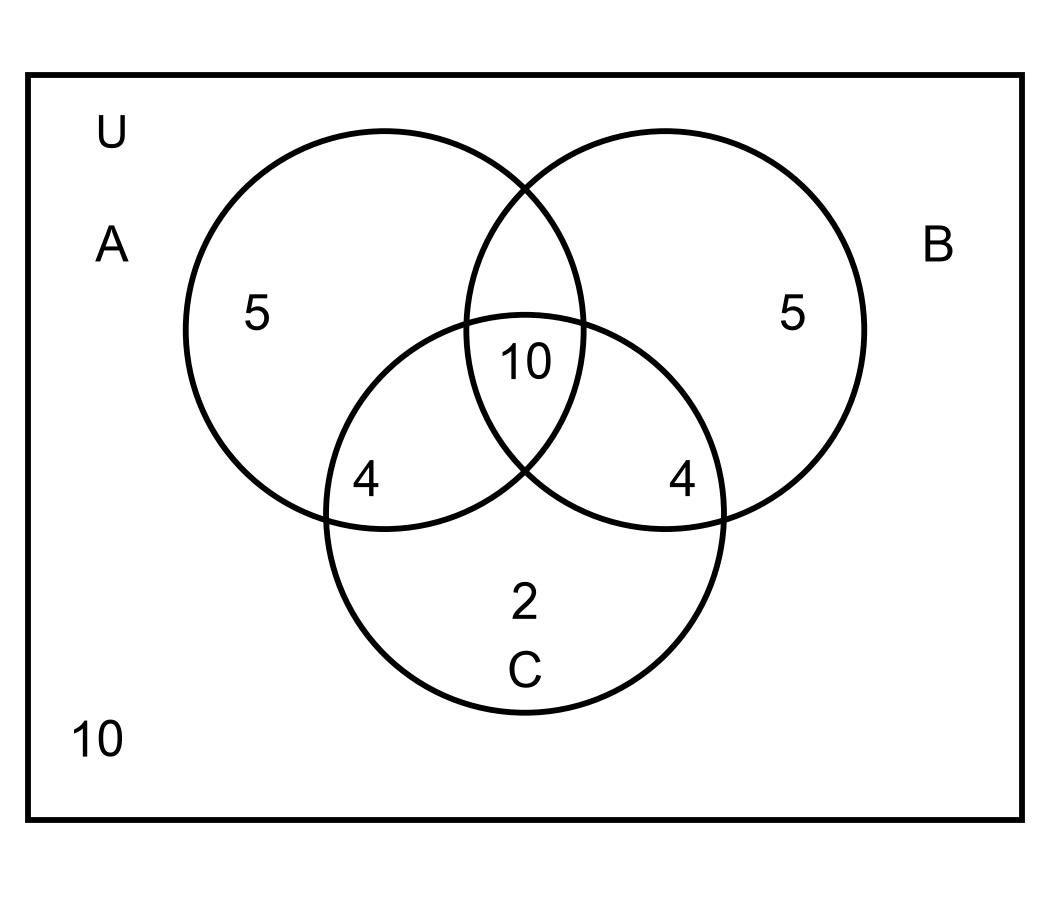
\includegraphics[width=0.38\textwidth]{figures/venn_50_ABC.png}
\end{center}
\step{所以单选物理、化学的人数至多 10 人.}
\step{所以至多选选择物理和化学这两门课程的学生人数至多 $10+10=20$ 人.}
\step{故选 C.}
\solend

\fi

\item 设 $k\geqslant 1,\,k\in\mathbb{N}$，已知集合 $M=\{1,2,3,4,5\}$，若集合 $N_1,N_2,\dots,N_k$ 是集合 $M$ 的 $k$ 个不同非空子集，且 $N_1\cup N_2\cup\dots\cup N_k\neq M$，则 $k$ 的最大值为\mbox{（\quad）.}

\keepwithprev
A. $15$\qquad B. $16$\qquad C. $31$\qquad D. $32$

\ans{A}

\ifanswer
\solbegin
\step{由 $N_1\cup N_2\cup\dots\cup N_k\neq M$ 得所有非空子集的并集缺少集合 $M$ 中至少一个元素.}
\step{假设缺少元素 1，则所有非空子集 $N_i$ 均不含元素 1，即 $N_i$ 是集合 $\{2,3,4,5\}$ 非空子集，集合 $\{2,3,4,5\}$ 的非空子集个数为 $2^4-1=15$，且这些子集 $N_i$ 的并集必不含 1，满足条件.}
\step{假设 $k\geqslant 16$，要满足所有非空子集的并集不等于集合 $M$，必须至少有一个集合 $M$ 中的元素不在任何一个子集中，否则并集就会等于 $M$.}
\step{设这个缺失的元素是 1，那么 $k$ 个非空集都不含元素 1，即每个子集都是集合 $\{2,3,4,5\}$ 的非空子集.}
\step{而集合 $\{2,3,4,5\}$ 只有 $2^4-1=15$ 个不同的非空子集，所以无法从中取出至少 16 个不同的非空子集.}
\step{因此假设不成立，$k$ 必须小于 16.}
\step{所以 $k$ 的最大值为 15，故选 A.}
\solend

\fi

% 注：原卷此题的差集记号是反斜杠 $A\setminus B$（本稿曾误作 $A\vee B$）；$C$ 的集合描述里原卷留了一条
%     待填横线“$x\in A\underline{\quad}B$”（选项按填入的符号分四种情形），本稿曾误作 $\vee\vee$。
%     2026-09-15 回原图核对时已按原卷改回。
\item 对于集合 $A$、$B$，定义 $A\setminus B=\{x\mid x\in A\text{ 且 }x\notin B\}$，则对于集合 $A=\{x\mid x=6n+5,\,n\in\mathbb{N}\}$，$B=\{y\mid y=3m+7,\,m\in\mathbb{N}\}$，$C=\{x\mid x\in A\underline{\hspace{4em}}B\text{ 且 }x<1000\}$，以下说法正确的是\mbox{（\quad）.}

\keepwithprev
A. 若在横线上填入“$\cap$”，则 $C$ 的真子集有 $2^{12}-1$ 个；

B. 若在横线上填入“$\cup$”，则 $C$ 中元素个数大于 250；

C. 若在横线上填入“$\setminus$”，则 $C$ 的非空真子集有 $2^{153}-2$ 个；

% 注：原卷选项 D 作“若在横线上填入“$\cup\complement_{\mathbb N}$”，则 $\complement_{\mathbb N}C$ 中元素个数为 13”；
%     本稿曾把 $\complement_{\mathbb N}$ 抄成 $\varnothing$、把 $\complement_{\mathbb N}C$ 抄成 $C\setminus C$，2026-09-15 回原图核对时已订正。
D. 若在横线上填入“$\cup\complement_{\mathbb{N}}$”，则 $\complement_{\mathbb{N}}C$ 中元素个数为 13.

\ans{B}

\ifanswer
\solbegin
\step{$x=6n+5=3(2n+1)+2$，$y=3m+7=3(m+2)+1$，集合 $A$、$B$ 无公共元素.}
\step{选项 A 中，集合 $C$ 为空集，没有真子集，$A$ 错；}
\step{选项 B 中，由 $6n+5<1000$ 得 $n<165\tfrac{5}{6}$，由 $3m+7<1000$ 得 $m<331$，因此 $C$ 中元素个数为 $166+331=497$，B 正确；}
\step{选项 C 中，$C$ 中元素个数为 166，非空真子集个数为 $2^{166}-2$，C 错；}
% 注：原卷此行作“$\complement_{\mathbb N}C=\complement_{\mathbb N}(A\cup\complement_{\mathbb N}B)
%     =\complement_{\mathbb N}A\cap\complement_{\mathbb N}(\complement_{\mathbb N}B)=\complement_{\mathbb N}A\cap B$，
%     而 $B\subseteq\complement_{\mathbb N}A$”；本稿曾把 $\complement_{\mathbb N}$ 抄成 $C\setminus$，同日已订正。
\step{选项 D 中，$\complement_{\mathbb{N}}C=\complement_{\mathbb{N}}(A\cup\complement_{\mathbb{N}}B)=\complement_{\mathbb{N}}A\cap\complement_{\mathbb{N}}(\complement_{\mathbb{N}}B)=\complement_{\mathbb{N}}A\cap B$，而 $B\subseteq\complement_{\mathbb{N}}A$.}
\step{因此其中元素个数为 331 个，D 错.}
\step{故选 B.}
\solend

\fi
\end{enumerate}

\bigsec{三、解答题}

\begin{enumerate}
\setcounter{enumi}{16}

\item 已知集合 $A=\{x\mid x<-1\text{ 或 }x>4\}$，$B=\{x\mid m+1\leqslant x\leqslant 2m+4\}$.
\begin{enumerate}[label=(\arabic*)]
\item 若 $m=2$，求 $A\cup B$ 和 $\left(\complement_{\R} A\right)\cap B$；
\item 若 $A\cap B=\varnothing$，求 $m$ 的取值范围.
\end{enumerate}

\ans{（1）$A\cup B=\{x\mid x<-1\text{ 或 }x\geqslant 3\}$，$\left(\complement_{\R} A\right)\cap B=\{x\mid 3\leqslant x\leqslant 4\}$；（2）$(-\infty,-3)\cup[-2,0]$}

\ifanswer
\solbegin
\stepm{(1)}{当 $m=2$ 时，集合 $B=\{x\mid 3\leqslant x\leqslant 8\}$.}
\step{又因为 $A=\{x\mid x<-1\text{ 或 }x>4\}$，则 $\complement_{\R}A=\{x\mid -1\leqslant x\leqslant 4\}$，所以 $A\cup B=\{x\mid x<-1\text{ 或 }x\geqslant 3\}$，$\left(\complement_{\R} A\right)\cap B=\{x\mid 3\leqslant x\leqslant 4\}$.}
\stepm{(2)}{因为 $A\cap B=\varnothing$，所以当 $B=\varnothing$ 时，$m+1>2m+4$，解得 $m<-3$ 满足题意；}
\step{当 $B\neq\varnothing$ 时，要满足题意，只需 $\begin{cases}m+1\leqslant 2m+4 \\ m+1\geqslant -1 \\ 2m+4\leqslant 4\end{cases}$，解得 $-2\leqslant m\leqslant 0$.}
\step{综上，实数 $m$ 的范围为 $m<-3$ 或 $-2\leqslant m\leqslant 0$，即 $(-\infty,-3)\cup[-2,0]$.}
\solend

\fi
\ansspace[6]
\item 设集合 $A=\{x\mid x^2+4x=0\}$，$B=\{x\mid x^2+2(a+1)x+a^2-1=0\}$.
\begin{enumerate}[label=(\arabic*)]
\item 写出集合 $A$ 的所有子集；
\item 若 $A\cap B=B$，求实数 $a$ 的取值范围.
\end{enumerate}

\ans{（1）$\{\varnothing,\{0\},\{-4\},\{0,-4\}\}$；（2）$a=1$ 或 $a\leqslant -1$}

\ifanswer
\solbegin
% 注：原卷此行印作“集合 $A$ 的所有子集为 $\varnothing,\{0\},\{-4\},\{0-4\}$”（末项漏逗号、且未加外层花括号）；
%     本稿按规范的列举写法给出，2026-09-15 回原图核对时加注。
\stepm{(1)}{由题意得 $A=\{0,-4\}$，集合 $A$ 的所有子集为 $\varnothing,\{0\},\{-4\},\{0,-4\}$.}
\stepm{(2)}{由 $A\cap B=B$ 得 $B\subseteq A$，所以 $B=\{0\}$ 或 $B=\{-4\}$ 或 $B=\{0,-4\}$ 或 $B=\varnothing$.}
\step{若 $B=\{0\}$ 时，$x^2+2(a+1)x+a^2-1=0$ 有两个相等的根 $0$，则 $\begin{cases}-2(a+1)=0 \\ a^2-1=-4\times(-4)\end{cases}$，解得 $a=-1$.}
\step{若 $B=\{-4\}$ 时，$x^2+2(a+1)x+a^2-1=0$ 有两个相等的根 $-4$，则 $\left\{\begin{matrix}-2(a+1)=-8 \\ a^2-1=-4\times(-4)\end{matrix}\right.$，$a$ 无解.}
\step{若 $B=\{0,-4\}$ 时，$x^2+2(a+1)x+a^2-1=0$ 有两个不相等的根 $0$ 和 $-4$，则 $\begin{cases}-2(a+1)=-4 \\ a^2-1=0\end{cases}$，解得 $a=1$.}
\step{当 $B=\varnothing$ 时，$x^2+2(a+1)x+a^2-1=0$ 无实数根，$\Delta=[2(a+1)]^2-4(a^2-1)=8a+8<0$，得 $a<-1$.}
\step{综上，$a=1$ 或 $a\leqslant -1$.}
\solend

\fi
\ansspace[6]
\item 已知集合 $A=\{x\mid x^2-5x+6=0\}$，$B=\{x\mid mx+1=0\}$，$C=\{x\in\mathbb{N}\mid \sqrt{x}\leqslant 1\}$，且 $A\cup B=A$.
\begin{enumerate}[label=(\arabic*)]
\item 求集合 $M=\{x\mid x\subseteq A\}$ 的真子集的个数；
\item 求实数 $m$ 的值组成的集合；
% 注：原卷本题的定义作“集合 $E=\{x\mid -x\in D,\,2-x^2\notin D\}$”；本稿曾把 $\notin$ 抄成 $\in$
%     （那样 $E=\varnothing$，与答案 $-5$ 冲突），2026-09-15 回原图核对时已订正。
\item 若集合 $D=A\cup C$，定义：集合 $E=\{x\mid -x\in D,\,2-x^2\notin D\}$，求集合 $E$ 中所有元素的和.
\end{enumerate}

\ans{（1）$15$；（2）$\left\{0,-\tfrac{1}{2},-\tfrac{1}{3}\right\}$；（3）$-5$}

\ifanswer
\solbegin
\stepm{(1)}{$A=\{x\mid x^2-5x+6=0\}=\{2,3\}$.}
\step{由 $M=\{x\mid x\subseteq A\}$ 得 $M$ 是 $A$ 的所有子集构成的集合，集合 $A$ 有 2 个元素，故 $A$ 的子集共 $2^2=4$ 个，即 $M$ 含 4 个元素，$M$ 的真子集个数为 $2^4-1=15$.}
\stepm{(2)}{由 (1) 得 $A=\{2,3\}$，集合 $B=\{x\mid mx+1=0\}$.}
\step{由 $A\cup B=A$ 得 $B\subseteq A$，分两种情况：① 当 $m=0$ 时，方程 $mx+1=0$ 无解，$B=\varnothing$，空集是任意集合的子集，符合条件；}
\stepm{②}{当 $m\neq 0$ 时，$B=\{-\tfrac{1}{m}\}$，由 $B\subseteq A$ 得 $-\tfrac{1}{m}=2$ 或 $-\tfrac{1}{m}=3$，解得 $m=-\tfrac{1}{2}$ 或 $m=-\tfrac{1}{3}$.}
\step{实数 $m$ 的取值集合为 $\left\{0,-\tfrac{1}{2},-\tfrac{1}{3}\right\}$.}
\stepm{(3)}{由 (1) 得 $A=\{2,3\}$.}
\step{由 $x\in\mathbb{N}$ 且 $\sqrt{x}\leqslant 1$，得 $x=0$ 或 $x=1$，故 $C=\{0,1\}$.}
\step{所以 $D=A\cup C=\{0,1,2,3\}$.}
\step{由 $-x\in D$ 得 $x$ 的候选值为 $0,-1,-2,-3$.}
\step{由于集合 $E=\{x\mid -x\in D,\,2-x^2\in D\}$，当 $x=0$ 时，$2-x^2=2\in D$，不符合题意；}
\step{当 $x=-1$ 时，$2-x^2=1\in D$，不符合题意；}
\step{当 $x=-2$ 时，$2-x^2=-2\notin D$，符合题意；}
\step{当 $x=-3$ 时，$2-x^2=-7\notin D$，符合题意.}
\step{故 $E=\{-2,-3\}$，所有元素的和为 $-2+(-3)=-5$.}
\solend

\fi
\ansspace[8]
\item 设集合 $M$ 是至少含有两个元素的数集，若 $M$ 中存在两个元素 $x$、$y$ 满足它们的积 $xy\in M$，则称 $M$ 为可积数集.
\begin{enumerate}[label=(\arabic*)]
\item 设集合 $A=\{2,3,5\}$，试判断 $A$ 是否为可积数集？并说明理由；
\item 设集合 $B=\{2,3,4,a\}$，若 $B$ 为可积数集，求实数 $a$ 的取值集合；
\item 设集合 $D=\{x\mid t<x<t+2\}$，若 $D$ 不是可积数集，求实数 $t$ 的取值范围.
\end{enumerate}

% 注：原卷本题【答案】与文末解析的结论都含 $\frac{3}{4}$；本稿曾漏掉 $\frac{3}{4}$
%     （与本稿自己的解析结论不一致），2026-09-15 回原图核对时已订正。
\ans{（1）否；（2）$\left\{0,\tfrac{1}{2},\tfrac{2}{3},\tfrac{3}{4},1,\tfrac{4}{3},\tfrac{3}{2},6,8,12\right\}$；（3）$t\in(-\infty,-2]\cup[2,+\infty)$}

\ifanswer
\solbegin
\stepm{(1)}{因为 $2\times 3=6\notin A$，$2\times 5=10\notin A$，$3\times 5=15\notin A$，所以 $A$ 中任意两个元素的积都不是 $A$ 中的元素，即 $A$ 不是可积数集.}
\stepm{(2)}{若 $B=\{2,3,4,a\}$ 为可积数集，则 $2\times 3=6\in B$，或 $2\times 4=8\in B$ 或 $3\times 4=12\in B$ 或 $2a\in B$ 或 $3a\in B$ 或 $4a\in B$.}
\step{若 $6\in B$，则 $a=6$；}
\step{若 $8\in B$，则 $a=8$；}
\step{若 $12\in B$，则 $a=12$；}
\step{若 $2a\in B$，则 $2a=2$ 或 $2a=3$ 或 $2a=4$ 或 $2a=a$，解得 $a=1$ 或 $a=\tfrac{3}{2}$ 或 $a=2$（舍）或 $a=0$；}
\step{若 $3a\in B$，则 $3a=2$ 或 $3a=3$ 或 $3a=4$ 或 $3a=a$，解得 $a=\tfrac{2}{3}$ 或 $a=1$ 或 $a=\tfrac{4}{3}$ 或 $a=0$；}
\step{若 $4a\in B$，则 $4a=2$ 或 $4a=3$ 或 $4a=4$ 或 $4a=a$，解得 $a=\tfrac{1}{2}$ 或 $a=\tfrac{3}{4}$ 或 $a=1$ 或 $a=0$.}
\step{综上，实数 $a$ 的取值集合为 $\left\{0,\tfrac{1}{2},\tfrac{2}{3},\tfrac{3}{4},1,\tfrac{4}{3},\tfrac{3}{2},6,8,12\right\}$.}
\stepm{(3)}{若 $D=\{x\mid t<x<t+2\}$ 不是可积数集，则 $\forall x,y\in(t,t+2)$，$xy\notin(t,t+2)$.}
\step{当 $t+2\leqslant 0$，即 $t\leqslant -2$ 时，$0\leqslant(t+2)^2<xy<t^2$，此时 $xy\notin D$，满足题意；}
\step{当 $t\geqslant 0$ 时，$0\leqslant t^2<xy<(t+2)^2$，因为 $(t+2)^2>t$，所以若 $xy\notin D$，则 $t^2\geqslant t+2$，即 $t^2-t-2\geqslant 0$，解得 $t\geqslant 2$ 或 $t\leqslant -1$，此时 $t\geqslant 2$ 满足题意；}
% 注：原卷此句作“当 $t<0<t+2$，即 $-2<t<0$ 时，$\exists x=0$，$xy=0\in D$，不满足题意，舍去”；
%     本稿曾把 $\in D$ 抄成 $\notin D$（$-2<t<0$ 时 $0\in(t,t+2)$，确有 $0\in D$），同日已订正。
\step{当 $t<0<t+2$，即 $-2<t<0$ 时，$\exists x=0$，$xy=0\in D$，不满足题意，舍去.}
\step{综上，所求实数 $t$ 的取值范围为 $t\geqslant 2$ 或 $t\leqslant -2$，故 $t\in(-\infty,-2]\cup[2,+\infty)$.}
\solend

\fi
\ansspace[8]
\ansneed{7cm}
\item 已知集合 $A$ 为非空数集，定义：$S=\{x\mid x=a+b,\,a,b\in A\}$，$T=\{x\mid x=|a-b|,a,b\in A\}$（实数 $a$、$b$ 可以相同）.
\begin{enumerate}[label=(\arabic*)]
\item 若集合 $A=\{2,5\}$，直接写出集合 $S$、$T$；
\item 若集合 $A=\{x_1,x_2,x_3,x_4\}$，$x_1<x_2<x_3<x_4$，且 $T=A$，求证：$x_1+x_4=x_3+x_2$；
\item 若集合 $A\subseteq\{x\mid 0\leqslant x\leqslant 2025,\,x\in\mathbb{N}\}$，$S\cap T=\varnothing$，记 $|A|$ 为集合 $A$ 中的元素个数，求 $|A|$ 的最大值.
\end{enumerate}

\ans{（1）$S=\{4,7,10\}$，$T=\{0,3\}$；（2）略；（3）$1350$}

\ifanswer
\solbegin
\stepm{(1)}{$S=\{4,7,10\}$，$T=\{0,3\}$.}
\stepm{(2)}{由集合 $A=\{x_1,x_2,x_3,x_4\}$，$x_1<x_2<x_3<x_4$，则 $T$ 集合的元素在 $0,x_2-x_1,x_3-x_1,x_4-x_1,x_3-x_2,x_4-x_2,x_4-x_3$ 中，且 $0<x_2-x_1<x_3-x_1<x_4-x_1$，$x_3-x_2<x_4-x_2<x_4-x_3$，因为 $A=T$，所以 $A$ 中最大元素 $x_4$ 必在 $T$ 中，而 $x_4-x_1$ 为 7 个元素中的最大者.}
\step{故 $x_4=x_4-x_1$，即 $x_1=0$.}
\step{故 $A=\{0,x_2,x_3,x_4\}$.}
\step{则 $x_3-x_2$、$x_4-x_2$、$x_4-x_3$ 与 $x_2$、$x_3$、$x_4$ 重复.}
\step{而 $0<x_3-x_2<x_3$，故 $x_3-x_2=x_2$，即 $x_3=2x_2$.}
% 注：原卷此句作“而 $0<x_4-x_3<x_4$，故 $x_4-x_3=x_2$ 或 $x_4-x_3=x_3$”；本稿曾把上界写成 $x_3$
%     （那样排除不了 $x_4-x_3=x_3$，与后半句自相矛盾），2026-09-15 回原图核对时已订正。
\step{而 $0<x_4-x_3<x_4$，故 $x_4-x_3=x_2$ 或 $x_4-x_3=x_3$.}
\step{若 $x_4=2x_3=4x_2$，则 $A=\{0,x_2,2x_2,4x_2\}$，$4x_2-x_2=3x_2\notin T$，与题设矛盾.}
\step{故 $x_4-x_3=x_2$，又因为 $x_1=0$，所以 $x_4+x_1=x_3+x_2$.}
% 注：原卷此行作“则 $2a_1<a_1+a_2<a_1+a_3<\cdots<a_1+a_k<a_2+a_k<a_3+a_k<\cdots<a_{k-1}+a_k<2a_k$，
%     所以 $|S|\geqslant 2k-1$，$a_1-a_1<a_2-a_1<a_3-a_1<\cdots<a_k-a_1$，所以 $|T|\geqslant k$”；
%     本稿曾把这个不等式链抄乱（作 $\cdots<a_1+a_k<a_2+a_3<a_k+a_k\leqslant 2a_k$）且把首项写成 $a_i-a_1$，
%     2026-09-15 回原图核对时已订正。
\stepm{(3)}{设 $A=\{a_1,a_2,\dots,a_k\}$ 满足题意，其中 $a_1<a_2<\dots<a_k$，则 $2a_1<a_1+a_2<a_1+a_3<\dots<a_1+a_k<a_2+a_k<a_3+a_k<\dots<a_{k-1}+a_k<2a_k$，所以 $|S|\geqslant 2k-1$，$a_1-a_1<a_2-a_1<a_3-a_1<\dots<a_k-a_1$，所以 $|T|\geqslant k$.}
\step{因为 $S\cap T=\varnothing$，由容斥原理得 $|S\cup T|=|S|+|T|\geqslant 3k-1$.}
\step{$S\cup T$ 中最小的元素为 0，最大的元素为 $2a_k$，$|S\cup T|\leqslant 2a_k+1$，所以 $3k-1\leqslant 2a_k+1\leqslant 2\times 2025+1\,(k\geqslant 1,k\in\mathbb{N})$，即 $3k-1\leqslant 4051$，解得 $k\leqslant 1350\tfrac{2}{3}$.}
\step{实际上 $A=\{676,677,678,\dots,2025\}$ 时满足题意，证明如下：设 $A=\{m,m+1,m+2,\dots,2025\}$，$m\in\mathbb{N}$.}
\step{则 $S=\{2m,2m+1,2m+2,\dots,4050\}$，$T=\{0,1,2,\dots,2025-m\}$.}
\step{由题意得 $2025-m<2m$，即 $m>675$.}
\step{所以 $A=\{676,677,678,\dots,2025\}$ 时满足题意，此时集合 $A$ 中的元素的个数最多.}
\step{综上所述，集合 $A$ 中元素的个数的最大值是 1350.}
\solend

\fi
\ansspace*[10]
\end{enumerate}

\end{document}"
% 紧凑版：xelatex "\def\iscompact{1}% 高一07_交附闵行_周练1.tex —— 高一上数学“2026-2027 年交附闵行高一上周练 1”（试卷版/答案版）
% 试卷版：xelatex 高一07_交附闵行_周练1.tex
% 答案版：xelatex "\def\isanswer{1}% 高一07_交附闵行_周练1.tex —— 高一上数学“2026-2027 年交附闵行高一上周练 1”（试卷版/答案版）
% 试卷版：xelatex 高一07_交附闵行_周练1.tex
% 答案版：xelatex "\def\isanswer{1}\input{高一07_交附闵行_周练1.tex}"
% 紧凑版：xelatex "\def\iscompact{1}\input{高一07_交附闵行_周练1.tex}"
%
% 原始材料是微信公众号图文（“魔都数学加油站”，作者署名“破晓”），正文为 11 张 PNG 页
% （1080×1527）；卷面上的粉色斜水印“魔都数学加油站”属水印，未录入。原文本身就是一份
% **讲评版**——题下直接印出【答案】或【解析】，本稿把这些答案与解析移到答案版，试卷版即
% 一张干净的空卷。
%
% 与原卷的排版差异（均已在 README“说明”中交代）：
%   ① 原文自**第 3 题**起（第 1、2 题未在该文发布），源码里以 \setcounter{enumi}{2} 起编；
%   ② 原卷本就印有分节标题“一、填空题”“二、选择题”“三、解答题”（已在原图上逐页放大
%      核对过），本稿照原卷分节，只把标题改排成全稿统一的“大节标题”样式；
%   ③ 原卷的实数集、整数集符号作正体 $R$（第 7 题）、$Z$（第 11 题），本稿按全稿惯例统一
%      写作 $\R$、$\Z$；
%   ④ 第 14 题【解析】里的 Venn 图取自原卷截图（`figures/venn_50_ABC.png`，4× LANCZOS
%      放大），未用 TikZ 重绘.

\documentclass[a4paper,11pt]{article}
\usepackage{common}

\begin{document}

\examtitlest{2026--2027 学年度交附闵行高一上周练 1}{集合与常用逻辑用语}

\bigsec{一、填空题}

\begin{enumerate}
\setcounter{enumi}{2}

\item 已知集合 $A=\{2,14,x^2+5\}$，$B=\{2,2x\}$，若 $A\cap B=B$，则实数 $x=$ \blankline[2em].

\ans{$7$}

\ifanswer
\solbegin
\step{因为 $A\cap B=B$，所以 $B\subseteq A$，所以 $2x=14$ 或 $x^2+5=2x$.}
\step{$2x=14$ 时，$x=7$，此时 $A=\{2,14,54\}$，$B=\{2,14\}$ 满足题意；}
\step{$x^2+5=2x$ 时，$(x-1)^2+4=0$，无解.}
\step{所以 $x=7$.}
\solend

\fi
\item 设集合 $A=\{y\mid y=x^2-1\}$，$B=\{(x,y)\mid y=x\}$，则 $A\cap B=$ \blankline[2em].

\ans{$\varnothing$}

\item 若集合 $\{0,-1,2a\}=\{a-1,-|a|,a+1\}$，实数 $a$ 的值为 \blankline[2em].

\ans{$\pm 1$}

\ifanswer
\solbegin
\step{令 $A=\{0,-1,2a\}$，$B=\{a-1,-|a|,a+1\}$，因为 $\{0,-1,2a\}=\{a-1,-|a|,a+1\}$，若 $a-1=0$，则 $a=1$，则 $A=\{0,-1,2\}$，$B=\{0,-1,2\}$，满足要求；}
\step{若 $-|a|=0$，则 $a=0$，则 $A=\{0,-1,0\}$，不满足集合元素的互异性；}
\step{若 $a+1=0$，则 $a=-1$，则 $A=\{0,-1,-2\}$，$B=\{0,-1,-2\}$，满足要求.}
\step{故实数 $a$ 的值为 $\pm 1$.}
\solend

\fi
\item 已知全集 $U=(-4,3]$，$A=\{x\in U\mid x^2+2x-8=0\}$，$B=\{x\in U\mid -3<1-2x\leqslant 5\}$，则 $\left(\complement_U B\right)\cap A=$ \blankline[2em].

\ans{$\{2\}$}

\item 已知集合 $A=\{x\mid 1-a\leqslant x\leqslant 1+a,\,a\in\R\}$ 中只有一个整数元素，则实数 $a$ 的取值范围为 \blankline[2em].

\ans{$[0,1)$}

\ifanswer
\solbegin
\step{集合 $A=\{x\mid 1-a\leqslant x\leqslant 1+a,\,a\in\R\}$ 中只有一个整数元素，则 $A\neq\varnothing,\,1-a\leqslant 1+a$，即 $a\geqslant 0$，此时 $1\in A$，故 $\begin{cases}1+a<2 \\ 1-a>0\end{cases}$，解得 $a<1$.}
\step{故 $a\in[0,1)$.}
\solend

\fi
\item 已知全集 $U=\{x\in\mathbb{N}\mid x\leqslant 9\}$，$A\cap B=\{3\}$，$\overline{A}\cap B=\{4,6,8\}$，$A\cap\overline{B}=\{1,5\}$，则 $\overline{A}=$ \blankline[2em].

\ans{$\{0,2,4,6,7,8,9\}$}

\ifanswer
\solbegin
\step{由题意得 $U=\{x\in\mathbb{N}\mid x\leqslant 9\}=\{0,1,2,3,4,5,6,7,8,9\}$，$A\cap B=\{3\}$ 得 $A$、$B$ 中含有元素 $3$；}
\step{$\overline{A}\cap B=\{4,6,8\}$ 得 $B$ 中含有 $4$、$6$、$8$，集合 $A$ 中不含 $4$、$6$、$8$；}
\step{$A\cap\overline{B}=\{1,5\}$ 得 $A$ 含有 $1$、$5$，集合 $B$ 不含 $1$、$5$.}
\step{对于 $0$，假设集合 $A$ 中含有 $0$，由 $A\cap B=\{3\}$ 得 $B$ 不含 $0$，则 $A\cap\overline{B}$ 必含元素 $0$，与 $A\cap\overline{B}=\{1,5\}$ 矛盾.}
\step{同理可得集合 $A$ 中不含元素 $2$、$7$、$9$.}
\step{综上所述，$A=\{1,3,5\}$.}
\step{故 $\overline{A}=\{0,2,4,6,7,8,9\}$.}
\solend

\fi
\item 已知一个有四个数字元素的集合 $S$，$S$ 的所有子集的元素和（空集的元素和认为是 0）的总和为 16208，则 $S$ 的元素之和等于 \blankline[2em].

\ans{$2026$}

\ifanswer
\solbegin
\step{设 $S=\{a_1,a_2,a_3,a_4\}$，$S$ 的每个元素在所有子集中均出现 $2^3$ 次，故 $(a_1+a_2+a_3+a_4)\cdot 2^3=16208$，所以 $a_1+a_2+a_3+a_4=2026$，故 $S$ 的元素之和等于 2026.}
\solend

\fi
\item 已知集合 $M=\{x\in\mathbb{N}\mid 1\leqslant x\leqslant 12\}$，集合 $A_1$、$A_2$、$A_3$ 满足：① 每个集合都恰有 4 个元素；② $A_1\cup A_2\cup A_3=M$. 集合 $A_i\,(i=1,2,3)$ 中元素的最大值与最小值之和称为集合 $A_i$ 的特征数，记为 $X_i\,(i=1,2,3)$，则 $X_1+X_2+X_3$ 的最大值与最小值的积为 \blankline[2em].

\ans{$1485$}

\ifanswer
\solbegin
\step{集合 $M=\{x\in\mathbb{N}\mid 1\leqslant x\leqslant 12\}$ 中最小值为 1，最大值为 12.}
% 注：原卷此处印作“则 $A_1=13$”（原卷笔误，按上下文应为 $X_1=13$），本稿按 $X_1$ 规范，2026-09-15 回原图核对时加注。
\stepm{①}{若使 $X_1+X_2+X_3$ 取得最大值，不妨设 $A_1=\{1,2,3,12\}$，则 $X_1=13$，则剩余的数中最小值是 4，最大值是 11，令 $A_2=\{4,5,6,11\}$，则 $X_2=15$，则 $A_3=\{7,8,9,10\}$，$X_3=17$，则 $X_1+X_2+X_3$ 的最大值为 $13+15+17=45$；}
\stepm{②}{若使 $X_1+X_2+X_3$ 取得最小值，则 $A_1=\{1,4,5,6\}$，则 $X_1=7$，令 $A_2=\{2,7,8,9\}$，则 $X_2=11$，则 $A_3=\{3,10,11,12\}$，$X_3=15$，则此时 $X_1+X_2+X_3$ 的最小值为 $7+11+15=33$.}
\step{故 $X_1+X_2+X_3$ 的最大值与最小值的积为 $45\times 33=1485$.}
\solend

\fi
\item 对于集合 $M=\{a\mid a=x^2-y^2,\,x\in\Z,\,y\in\Z\}$，给出如下三个结论：

① 如果 $P=\{b\mid b=2n+1,\,n\in\Z\}$，那么 $P\subseteq M$；

% 注：原卷此条作“如果 $c=4n+2$，$n\in\Z$，那么 $c\notin M$”；本稿曾把 $\notin$ 抄成 $\in$
%     （那样②为假，与本卷答案 ①②③ 冲突），2026-09-15 回原图核对时已订正。
② 如果 $c=4n+2$，$n\in\Z$，那么 $c\notin M$；

③ 如果 $a_1\in M$，$a_2\in M$，那么 $a_1a_2\in M$. 其中正确结论的序号是 \blankline[2em].

\ans{①②③}

\ifanswer
\solbegin
\stepm{①}{由已知 $b=2n+1,\,n\in\Z$，则恒有 $2n+1=(n+1)^2-n^2,\,n\in\Z$，所以 $2n+1\in M$，所以 $P\subseteq M$，所以①正确；}
\stepm{②}{元素 $c=4n+2,\,n\in\Z$，若 $4n+2\in M$，则存在 $x$、$y\in\Z$ 使得 $x^2-y^2=4n+2$，所以 $4n+2=(x+y)(x-y)$，则 $x+y$ 与 $x-y$ 同奇或同偶.}
\step{若 $x+y$ 与 $x-y$ 都是奇数，则 $(x+y)(x-y)$ 为奇数，而 $4n+2$ 是偶数；}
\step{若 $x+y$ 和 $x-y$ 都是偶数，则 $(x+y)(x-y)$ 能被 4 整除，而 $4n+2$ 不能被 4 整除.}
\step{所以 $4n+2\notin M$，即 $c\notin M$，故②正确；}
\stepm{③}{因为 $a_1$、$a_2\in M$，则 $a_1a_2$ 还是整数，所以 $a_1a_2\in M$，故③正确.}
\step{故正确的是①②③.}
\solend

\fi
\item 用 $C(A)$ 表示非空集合 $A$ 中的元素的个数，定义 $A*B=|C(A)-C(B)|$，若 $A=\{x\mid x^2-2024x-2025=0\}$，$B=\{x\mid (2x^2+ax)(x^2+2ax+6)=0\}$，若 $A*B=1$，则 $a$ 的所有可能取值构成集合 $M$，则 $C(M)=$ \blankline[2em].

\ans{$5$}

\ifanswer
\solbegin
\step{$x^2-2024x-2025=0$ 得 $x=2025$ 或 $x=-1$，即 $C(A)=2$，因为 $A*B=|C(A)-C(B)|=1$，所以 $C(B)=3$ 或 $C(B)=1$.}
\step{方程 $(2x^2+ax)(x^2+2ax+6)=0$ 化为 $x(2x+a)(x^2+2ax+6)=0$.}
\step{当 $a=0$ 时，方程化为 $2x^3(x^2+6)=0$，解得 $x=0$，所以 $B=\{0\}$，$C(B)=1$，符合题意.}
\step{当 $a\neq 0$ 时，方程化为 $x=0$ 或 $x=-\tfrac{a}{2}$ 或 $x^2+2ax+6=0$.}
\step{因为 $0\neq -\tfrac{a}{2}$，$C(B)\neq 1$，故只有 $C(B)=3$.}
\step{故 $x^2+2ax+6=0$ 有两个相等的非零实数根，所以 $\Delta=4a^2-4\times 6=0$，解得 $a=\pm\sqrt{6}$，符合题意.}
\step{当 $x^2+2ax+6=0$ 有两个不相等实根，设 $x_1$、$x_2$，若 $x_1=-\tfrac{a}{2}$，由韦达定理得 $\begin{cases}x_1+x_2=-2a \\ x_1x_2=6\end{cases}$，% 注：原卷作“得 $x_2=-\frac{3a}{2}$”（由 $x_1+x_2=-2a$、$x_1=-\frac{a}{2}$ 得 $x_2=-\frac{3a}{2}$）；
%     本稿曾漏掉负号，2026-09-15 回原图核对时已订正。
得 $x_2=-\tfrac{3a}{2}$，$-\tfrac{a}{2}\cdot(-\tfrac{3a}{2})=\tfrac{3a^2}{4}=6$，解得 $a=\pm 2\sqrt{2}$，符合题意.}
\step{综上所述，$M=\{0,\sqrt{6},-\sqrt{6},2\sqrt{2},-2\sqrt{2}\}$，所以 $C(M)=5$.}
\solend

\fi
\end{enumerate}

\bigsec{二、选择题}

\begin{enumerate}
\setcounter{enumi}{12}

\item 已知集合 $A=\{1,2,3,4,5\}$，$B=\{x\mid \tfrac{x-1}{2}\in\Z,\,x\in A\}$，则集合 $B$ 的真子集个数为\mbox{（\quad）.}

\keepwithprev
A. $3$\qquad B. $5$\qquad C. $7$\qquad D. $15$

\ans{C}

\ifanswer
\solbegin
\step{已知集合 $A=\{1,2,3,4,5\}$，$B=\{x\mid\tfrac{x-1}{2}\in\Z,\,x\in A\}$.}
\step{因为 $\tfrac{x-1}{2}\in\Z$，所以 $x$ 为奇数，所以 $B=\{1,3,5\}$.}
\step{所以集合 $B$ 中有 3 个元素，所以集合 $B$ 的真子集个数为 $2^3-1=7$.}
\step{故选 C.}
\solend

\fi

\item 高一二班共有学生 50 人，每名学生要从物理、化学、生物、历史、地理、政治这六门课程中选择三门课程进行学习. 已知选择物理、化学、生物的学生各有至少 20 人，这三门课程都不选的有 10 人，这三门课程都选的有 10 人，在这三门课程中选择任意两门课程的都至少有 14 人，物理、化学只选一科的学生都至少 5 人，那么选择物理和化学这两门课程的学生人数至多\mbox{（\quad）.}

\keepwithprev
A. $18$\qquad B. $19$\qquad C. $20$\qquad D. $21$

\ans{C}

\ifanswer
\solbegin
\step{可以把学生 50 人看作一个集合 $U$，选择物理的人数组成集合 $A$，选择化学的人数组成集合 $B$，选择生物的人数组成集合 $C$.}
\step{要使选择物理和化学这两门课程的学生人数最多，除这三门课程都不选的有 10 人，这三门课程都选的有 10 人，则其他科选择人数均为最少，因为物理、化学只选一科的学生都至少 5 人，即得到单选物理的最少 5 人，单选化学的最少 5 人.}
\step{因为在这三门课程中选择任意两门课程的都至少有 14 人，单选化学、生物的最少 4 人，单选物理、生物的最少 4 人.}
\step{因为选择物理、化学、生物的学生各有至少 20 人，所以单选生物的最少 2 人.}
\step{以上人数最少 30 人，可作出如图所示的韦恩图：}
% 注：原卷此处印有一张韦恩图（三个圆 $A$、$B$、$C$，$A$ 独有 5、$B$ 独有 5、三集合公共 10、
%     $A\cap C$ 独有 4、$B\cap C$ 独有 4、$C$ 独有 2、三集合之外 10）；本稿此前漏排此图而正文仍作
%     “如图”，2026-09-15 回原图核对时按原卷截图补入（见 figures/venn_50_ABC.png）。
\begin{center}
% 插图取自原卷截图（裁去截图残影后 4× LANCZOS 放大），不用 TikZ 手绘
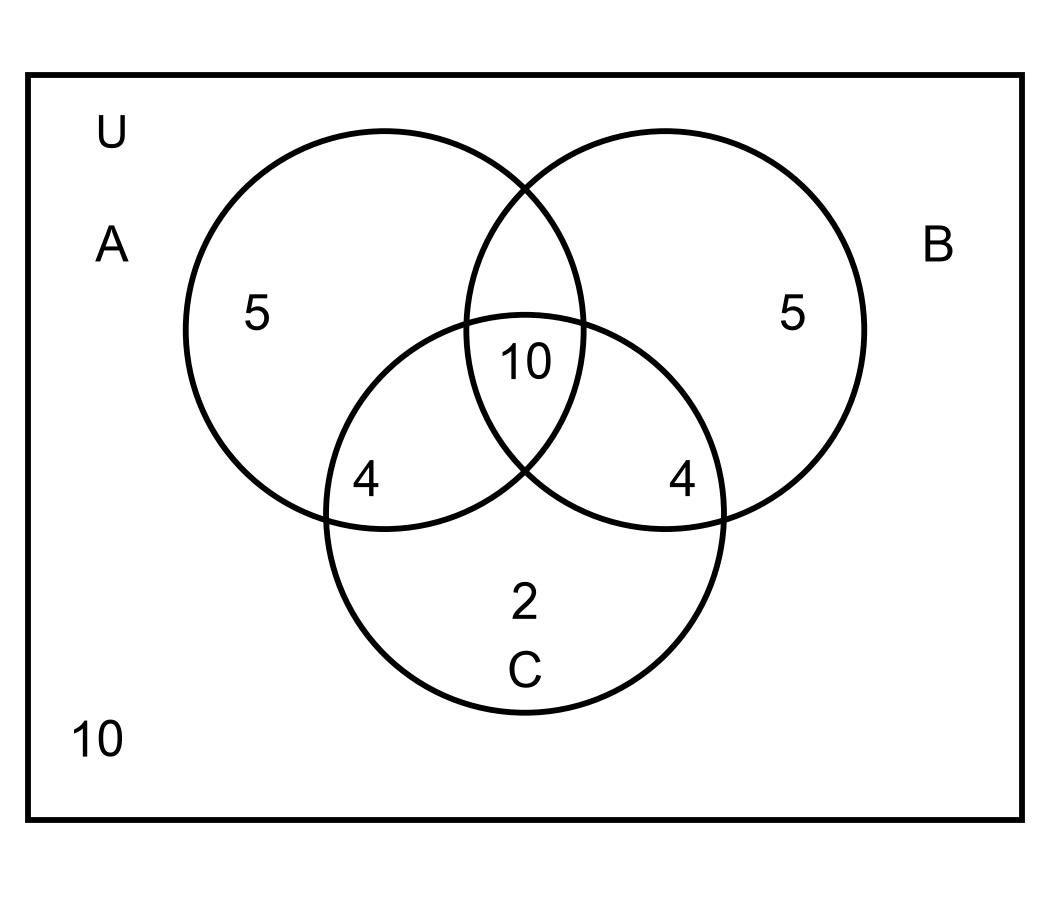
\includegraphics[width=0.38\textwidth]{figures/venn_50_ABC.png}
\end{center}
\step{所以单选物理、化学的人数至多 10 人.}
\step{所以至多选选择物理和化学这两门课程的学生人数至多 $10+10=20$ 人.}
\step{故选 C.}
\solend

\fi

\item 设 $k\geqslant 1,\,k\in\mathbb{N}$，已知集合 $M=\{1,2,3,4,5\}$，若集合 $N_1,N_2,\dots,N_k$ 是集合 $M$ 的 $k$ 个不同非空子集，且 $N_1\cup N_2\cup\dots\cup N_k\neq M$，则 $k$ 的最大值为\mbox{（\quad）.}

\keepwithprev
A. $15$\qquad B. $16$\qquad C. $31$\qquad D. $32$

\ans{A}

\ifanswer
\solbegin
\step{由 $N_1\cup N_2\cup\dots\cup N_k\neq M$ 得所有非空子集的并集缺少集合 $M$ 中至少一个元素.}
\step{假设缺少元素 1，则所有非空子集 $N_i$ 均不含元素 1，即 $N_i$ 是集合 $\{2,3,4,5\}$ 非空子集，集合 $\{2,3,4,5\}$ 的非空子集个数为 $2^4-1=15$，且这些子集 $N_i$ 的并集必不含 1，满足条件.}
\step{假设 $k\geqslant 16$，要满足所有非空子集的并集不等于集合 $M$，必须至少有一个集合 $M$ 中的元素不在任何一个子集中，否则并集就会等于 $M$.}
\step{设这个缺失的元素是 1，那么 $k$ 个非空集都不含元素 1，即每个子集都是集合 $\{2,3,4,5\}$ 的非空子集.}
\step{而集合 $\{2,3,4,5\}$ 只有 $2^4-1=15$ 个不同的非空子集，所以无法从中取出至少 16 个不同的非空子集.}
\step{因此假设不成立，$k$ 必须小于 16.}
\step{所以 $k$ 的最大值为 15，故选 A.}
\solend

\fi

% 注：原卷此题的差集记号是反斜杠 $A\setminus B$（本稿曾误作 $A\vee B$）；$C$ 的集合描述里原卷留了一条
%     待填横线“$x\in A\underline{\quad}B$”（选项按填入的符号分四种情形），本稿曾误作 $\vee\vee$。
%     2026-09-15 回原图核对时已按原卷改回。
\item 对于集合 $A$、$B$，定义 $A\setminus B=\{x\mid x\in A\text{ 且 }x\notin B\}$，则对于集合 $A=\{x\mid x=6n+5,\,n\in\mathbb{N}\}$，$B=\{y\mid y=3m+7,\,m\in\mathbb{N}\}$，$C=\{x\mid x\in A\underline{\hspace{4em}}B\text{ 且 }x<1000\}$，以下说法正确的是\mbox{（\quad）.}

\keepwithprev
A. 若在横线上填入“$\cap$”，则 $C$ 的真子集有 $2^{12}-1$ 个；

B. 若在横线上填入“$\cup$”，则 $C$ 中元素个数大于 250；

C. 若在横线上填入“$\setminus$”，则 $C$ 的非空真子集有 $2^{153}-2$ 个；

% 注：原卷选项 D 作“若在横线上填入“$\cup\complement_{\mathbb N}$”，则 $\complement_{\mathbb N}C$ 中元素个数为 13”；
%     本稿曾把 $\complement_{\mathbb N}$ 抄成 $\varnothing$、把 $\complement_{\mathbb N}C$ 抄成 $C\setminus C$，2026-09-15 回原图核对时已订正。
D. 若在横线上填入“$\cup\complement_{\mathbb{N}}$”，则 $\complement_{\mathbb{N}}C$ 中元素个数为 13.

\ans{B}

\ifanswer
\solbegin
\step{$x=6n+5=3(2n+1)+2$，$y=3m+7=3(m+2)+1$，集合 $A$、$B$ 无公共元素.}
\step{选项 A 中，集合 $C$ 为空集，没有真子集，$A$ 错；}
\step{选项 B 中，由 $6n+5<1000$ 得 $n<165\tfrac{5}{6}$，由 $3m+7<1000$ 得 $m<331$，因此 $C$ 中元素个数为 $166+331=497$，B 正确；}
\step{选项 C 中，$C$ 中元素个数为 166，非空真子集个数为 $2^{166}-2$，C 错；}
% 注：原卷此行作“$\complement_{\mathbb N}C=\complement_{\mathbb N}(A\cup\complement_{\mathbb N}B)
%     =\complement_{\mathbb N}A\cap\complement_{\mathbb N}(\complement_{\mathbb N}B)=\complement_{\mathbb N}A\cap B$，
%     而 $B\subseteq\complement_{\mathbb N}A$”；本稿曾把 $\complement_{\mathbb N}$ 抄成 $C\setminus$，同日已订正。
\step{选项 D 中，$\complement_{\mathbb{N}}C=\complement_{\mathbb{N}}(A\cup\complement_{\mathbb{N}}B)=\complement_{\mathbb{N}}A\cap\complement_{\mathbb{N}}(\complement_{\mathbb{N}}B)=\complement_{\mathbb{N}}A\cap B$，而 $B\subseteq\complement_{\mathbb{N}}A$.}
\step{因此其中元素个数为 331 个，D 错.}
\step{故选 B.}
\solend

\fi
\end{enumerate}

\bigsec{三、解答题}

\begin{enumerate}
\setcounter{enumi}{16}

\item 已知集合 $A=\{x\mid x<-1\text{ 或 }x>4\}$，$B=\{x\mid m+1\leqslant x\leqslant 2m+4\}$.
\begin{enumerate}[label=(\arabic*)]
\item 若 $m=2$，求 $A\cup B$ 和 $\left(\complement_{\R} A\right)\cap B$；
\item 若 $A\cap B=\varnothing$，求 $m$ 的取值范围.
\end{enumerate}

\ans{（1）$A\cup B=\{x\mid x<-1\text{ 或 }x\geqslant 3\}$，$\left(\complement_{\R} A\right)\cap B=\{x\mid 3\leqslant x\leqslant 4\}$；（2）$(-\infty,-3)\cup[-2,0]$}

\ifanswer
\solbegin
\stepm{(1)}{当 $m=2$ 时，集合 $B=\{x\mid 3\leqslant x\leqslant 8\}$.}
\step{又因为 $A=\{x\mid x<-1\text{ 或 }x>4\}$，则 $\complement_{\R}A=\{x\mid -1\leqslant x\leqslant 4\}$，所以 $A\cup B=\{x\mid x<-1\text{ 或 }x\geqslant 3\}$，$\left(\complement_{\R} A\right)\cap B=\{x\mid 3\leqslant x\leqslant 4\}$.}
\stepm{(2)}{因为 $A\cap B=\varnothing$，所以当 $B=\varnothing$ 时，$m+1>2m+4$，解得 $m<-3$ 满足题意；}
\step{当 $B\neq\varnothing$ 时，要满足题意，只需 $\begin{cases}m+1\leqslant 2m+4 \\ m+1\geqslant -1 \\ 2m+4\leqslant 4\end{cases}$，解得 $-2\leqslant m\leqslant 0$.}
\step{综上，实数 $m$ 的范围为 $m<-3$ 或 $-2\leqslant m\leqslant 0$，即 $(-\infty,-3)\cup[-2,0]$.}
\solend

\fi
\ansspace[6]
\item 设集合 $A=\{x\mid x^2+4x=0\}$，$B=\{x\mid x^2+2(a+1)x+a^2-1=0\}$.
\begin{enumerate}[label=(\arabic*)]
\item 写出集合 $A$ 的所有子集；
\item 若 $A\cap B=B$，求实数 $a$ 的取值范围.
\end{enumerate}

\ans{（1）$\{\varnothing,\{0\},\{-4\},\{0,-4\}\}$；（2）$a=1$ 或 $a\leqslant -1$}

\ifanswer
\solbegin
% 注：原卷此行印作“集合 $A$ 的所有子集为 $\varnothing,\{0\},\{-4\},\{0-4\}$”（末项漏逗号、且未加外层花括号）；
%     本稿按规范的列举写法给出，2026-09-15 回原图核对时加注。
\stepm{(1)}{由题意得 $A=\{0,-4\}$，集合 $A$ 的所有子集为 $\varnothing,\{0\},\{-4\},\{0,-4\}$.}
\stepm{(2)}{由 $A\cap B=B$ 得 $B\subseteq A$，所以 $B=\{0\}$ 或 $B=\{-4\}$ 或 $B=\{0,-4\}$ 或 $B=\varnothing$.}
\step{若 $B=\{0\}$ 时，$x^2+2(a+1)x+a^2-1=0$ 有两个相等的根 $0$，则 $\begin{cases}-2(a+1)=0 \\ a^2-1=-4\times(-4)\end{cases}$，解得 $a=-1$.}
\step{若 $B=\{-4\}$ 时，$x^2+2(a+1)x+a^2-1=0$ 有两个相等的根 $-4$，则 $\left\{\begin{matrix}-2(a+1)=-8 \\ a^2-1=-4\times(-4)\end{matrix}\right.$，$a$ 无解.}
\step{若 $B=\{0,-4\}$ 时，$x^2+2(a+1)x+a^2-1=0$ 有两个不相等的根 $0$ 和 $-4$，则 $\begin{cases}-2(a+1)=-4 \\ a^2-1=0\end{cases}$，解得 $a=1$.}
\step{当 $B=\varnothing$ 时，$x^2+2(a+1)x+a^2-1=0$ 无实数根，$\Delta=[2(a+1)]^2-4(a^2-1)=8a+8<0$，得 $a<-1$.}
\step{综上，$a=1$ 或 $a\leqslant -1$.}
\solend

\fi
\ansspace[6]
\item 已知集合 $A=\{x\mid x^2-5x+6=0\}$，$B=\{x\mid mx+1=0\}$，$C=\{x\in\mathbb{N}\mid \sqrt{x}\leqslant 1\}$，且 $A\cup B=A$.
\begin{enumerate}[label=(\arabic*)]
\item 求集合 $M=\{x\mid x\subseteq A\}$ 的真子集的个数；
\item 求实数 $m$ 的值组成的集合；
% 注：原卷本题的定义作“集合 $E=\{x\mid -x\in D,\,2-x^2\notin D\}$”；本稿曾把 $\notin$ 抄成 $\in$
%     （那样 $E=\varnothing$，与答案 $-5$ 冲突），2026-09-15 回原图核对时已订正。
\item 若集合 $D=A\cup C$，定义：集合 $E=\{x\mid -x\in D,\,2-x^2\notin D\}$，求集合 $E$ 中所有元素的和.
\end{enumerate}

\ans{（1）$15$；（2）$\left\{0,-\tfrac{1}{2},-\tfrac{1}{3}\right\}$；（3）$-5$}

\ifanswer
\solbegin
\stepm{(1)}{$A=\{x\mid x^2-5x+6=0\}=\{2,3\}$.}
\step{由 $M=\{x\mid x\subseteq A\}$ 得 $M$ 是 $A$ 的所有子集构成的集合，集合 $A$ 有 2 个元素，故 $A$ 的子集共 $2^2=4$ 个，即 $M$ 含 4 个元素，$M$ 的真子集个数为 $2^4-1=15$.}
\stepm{(2)}{由 (1) 得 $A=\{2,3\}$，集合 $B=\{x\mid mx+1=0\}$.}
\step{由 $A\cup B=A$ 得 $B\subseteq A$，分两种情况：① 当 $m=0$ 时，方程 $mx+1=0$ 无解，$B=\varnothing$，空集是任意集合的子集，符合条件；}
\stepm{②}{当 $m\neq 0$ 时，$B=\{-\tfrac{1}{m}\}$，由 $B\subseteq A$ 得 $-\tfrac{1}{m}=2$ 或 $-\tfrac{1}{m}=3$，解得 $m=-\tfrac{1}{2}$ 或 $m=-\tfrac{1}{3}$.}
\step{实数 $m$ 的取值集合为 $\left\{0,-\tfrac{1}{2},-\tfrac{1}{3}\right\}$.}
\stepm{(3)}{由 (1) 得 $A=\{2,3\}$.}
\step{由 $x\in\mathbb{N}$ 且 $\sqrt{x}\leqslant 1$，得 $x=0$ 或 $x=1$，故 $C=\{0,1\}$.}
\step{所以 $D=A\cup C=\{0,1,2,3\}$.}
\step{由 $-x\in D$ 得 $x$ 的候选值为 $0,-1,-2,-3$.}
\step{由于集合 $E=\{x\mid -x\in D,\,2-x^2\in D\}$，当 $x=0$ 时，$2-x^2=2\in D$，不符合题意；}
\step{当 $x=-1$ 时，$2-x^2=1\in D$，不符合题意；}
\step{当 $x=-2$ 时，$2-x^2=-2\notin D$，符合题意；}
\step{当 $x=-3$ 时，$2-x^2=-7\notin D$，符合题意.}
\step{故 $E=\{-2,-3\}$，所有元素的和为 $-2+(-3)=-5$.}
\solend

\fi
\ansspace[8]
\item 设集合 $M$ 是至少含有两个元素的数集，若 $M$ 中存在两个元素 $x$、$y$ 满足它们的积 $xy\in M$，则称 $M$ 为可积数集.
\begin{enumerate}[label=(\arabic*)]
\item 设集合 $A=\{2,3,5\}$，试判断 $A$ 是否为可积数集？并说明理由；
\item 设集合 $B=\{2,3,4,a\}$，若 $B$ 为可积数集，求实数 $a$ 的取值集合；
\item 设集合 $D=\{x\mid t<x<t+2\}$，若 $D$ 不是可积数集，求实数 $t$ 的取值范围.
\end{enumerate}

% 注：原卷本题【答案】与文末解析的结论都含 $\frac{3}{4}$；本稿曾漏掉 $\frac{3}{4}$
%     （与本稿自己的解析结论不一致），2026-09-15 回原图核对时已订正。
\ans{（1）否；（2）$\left\{0,\tfrac{1}{2},\tfrac{2}{3},\tfrac{3}{4},1,\tfrac{4}{3},\tfrac{3}{2},6,8,12\right\}$；（3）$t\in(-\infty,-2]\cup[2,+\infty)$}

\ifanswer
\solbegin
\stepm{(1)}{因为 $2\times 3=6\notin A$，$2\times 5=10\notin A$，$3\times 5=15\notin A$，所以 $A$ 中任意两个元素的积都不是 $A$ 中的元素，即 $A$ 不是可积数集.}
\stepm{(2)}{若 $B=\{2,3,4,a\}$ 为可积数集，则 $2\times 3=6\in B$，或 $2\times 4=8\in B$ 或 $3\times 4=12\in B$ 或 $2a\in B$ 或 $3a\in B$ 或 $4a\in B$.}
\step{若 $6\in B$，则 $a=6$；}
\step{若 $8\in B$，则 $a=8$；}
\step{若 $12\in B$，则 $a=12$；}
\step{若 $2a\in B$，则 $2a=2$ 或 $2a=3$ 或 $2a=4$ 或 $2a=a$，解得 $a=1$ 或 $a=\tfrac{3}{2}$ 或 $a=2$（舍）或 $a=0$；}
\step{若 $3a\in B$，则 $3a=2$ 或 $3a=3$ 或 $3a=4$ 或 $3a=a$，解得 $a=\tfrac{2}{3}$ 或 $a=1$ 或 $a=\tfrac{4}{3}$ 或 $a=0$；}
\step{若 $4a\in B$，则 $4a=2$ 或 $4a=3$ 或 $4a=4$ 或 $4a=a$，解得 $a=\tfrac{1}{2}$ 或 $a=\tfrac{3}{4}$ 或 $a=1$ 或 $a=0$.}
\step{综上，实数 $a$ 的取值集合为 $\left\{0,\tfrac{1}{2},\tfrac{2}{3},\tfrac{3}{4},1,\tfrac{4}{3},\tfrac{3}{2},6,8,12\right\}$.}
\stepm{(3)}{若 $D=\{x\mid t<x<t+2\}$ 不是可积数集，则 $\forall x,y\in(t,t+2)$，$xy\notin(t,t+2)$.}
\step{当 $t+2\leqslant 0$，即 $t\leqslant -2$ 时，$0\leqslant(t+2)^2<xy<t^2$，此时 $xy\notin D$，满足题意；}
\step{当 $t\geqslant 0$ 时，$0\leqslant t^2<xy<(t+2)^2$，因为 $(t+2)^2>t$，所以若 $xy\notin D$，则 $t^2\geqslant t+2$，即 $t^2-t-2\geqslant 0$，解得 $t\geqslant 2$ 或 $t\leqslant -1$，此时 $t\geqslant 2$ 满足题意；}
% 注：原卷此句作“当 $t<0<t+2$，即 $-2<t<0$ 时，$\exists x=0$，$xy=0\in D$，不满足题意，舍去”；
%     本稿曾把 $\in D$ 抄成 $\notin D$（$-2<t<0$ 时 $0\in(t,t+2)$，确有 $0\in D$），同日已订正。
\step{当 $t<0<t+2$，即 $-2<t<0$ 时，$\exists x=0$，$xy=0\in D$，不满足题意，舍去.}
\step{综上，所求实数 $t$ 的取值范围为 $t\geqslant 2$ 或 $t\leqslant -2$，故 $t\in(-\infty,-2]\cup[2,+\infty)$.}
\solend

\fi
\ansspace[8]
\ansneed{7cm}
\item 已知集合 $A$ 为非空数集，定义：$S=\{x\mid x=a+b,\,a,b\in A\}$，$T=\{x\mid x=|a-b|,a,b\in A\}$（实数 $a$、$b$ 可以相同）.
\begin{enumerate}[label=(\arabic*)]
\item 若集合 $A=\{2,5\}$，直接写出集合 $S$、$T$；
\item 若集合 $A=\{x_1,x_2,x_3,x_4\}$，$x_1<x_2<x_3<x_4$，且 $T=A$，求证：$x_1+x_4=x_3+x_2$；
\item 若集合 $A\subseteq\{x\mid 0\leqslant x\leqslant 2025,\,x\in\mathbb{N}\}$，$S\cap T=\varnothing$，记 $|A|$ 为集合 $A$ 中的元素个数，求 $|A|$ 的最大值.
\end{enumerate}

\ans{（1）$S=\{4,7,10\}$，$T=\{0,3\}$；（2）略；（3）$1350$}

\ifanswer
\solbegin
\stepm{(1)}{$S=\{4,7,10\}$，$T=\{0,3\}$.}
\stepm{(2)}{由集合 $A=\{x_1,x_2,x_3,x_4\}$，$x_1<x_2<x_3<x_4$，则 $T$ 集合的元素在 $0,x_2-x_1,x_3-x_1,x_4-x_1,x_3-x_2,x_4-x_2,x_4-x_3$ 中，且 $0<x_2-x_1<x_3-x_1<x_4-x_1$，$x_3-x_2<x_4-x_2<x_4-x_3$，因为 $A=T$，所以 $A$ 中最大元素 $x_4$ 必在 $T$ 中，而 $x_4-x_1$ 为 7 个元素中的最大者.}
\step{故 $x_4=x_4-x_1$，即 $x_1=0$.}
\step{故 $A=\{0,x_2,x_3,x_4\}$.}
\step{则 $x_3-x_2$、$x_4-x_2$、$x_4-x_3$ 与 $x_2$、$x_3$、$x_4$ 重复.}
\step{而 $0<x_3-x_2<x_3$，故 $x_3-x_2=x_2$，即 $x_3=2x_2$.}
% 注：原卷此句作“而 $0<x_4-x_3<x_4$，故 $x_4-x_3=x_2$ 或 $x_4-x_3=x_3$”；本稿曾把上界写成 $x_3$
%     （那样排除不了 $x_4-x_3=x_3$，与后半句自相矛盾），2026-09-15 回原图核对时已订正。
\step{而 $0<x_4-x_3<x_4$，故 $x_4-x_3=x_2$ 或 $x_4-x_3=x_3$.}
\step{若 $x_4=2x_3=4x_2$，则 $A=\{0,x_2,2x_2,4x_2\}$，$4x_2-x_2=3x_2\notin T$，与题设矛盾.}
\step{故 $x_4-x_3=x_2$，又因为 $x_1=0$，所以 $x_4+x_1=x_3+x_2$.}
% 注：原卷此行作“则 $2a_1<a_1+a_2<a_1+a_3<\cdots<a_1+a_k<a_2+a_k<a_3+a_k<\cdots<a_{k-1}+a_k<2a_k$，
%     所以 $|S|\geqslant 2k-1$，$a_1-a_1<a_2-a_1<a_3-a_1<\cdots<a_k-a_1$，所以 $|T|\geqslant k$”；
%     本稿曾把这个不等式链抄乱（作 $\cdots<a_1+a_k<a_2+a_3<a_k+a_k\leqslant 2a_k$）且把首项写成 $a_i-a_1$，
%     2026-09-15 回原图核对时已订正。
\stepm{(3)}{设 $A=\{a_1,a_2,\dots,a_k\}$ 满足题意，其中 $a_1<a_2<\dots<a_k$，则 $2a_1<a_1+a_2<a_1+a_3<\dots<a_1+a_k<a_2+a_k<a_3+a_k<\dots<a_{k-1}+a_k<2a_k$，所以 $|S|\geqslant 2k-1$，$a_1-a_1<a_2-a_1<a_3-a_1<\dots<a_k-a_1$，所以 $|T|\geqslant k$.}
\step{因为 $S\cap T=\varnothing$，由容斥原理得 $|S\cup T|=|S|+|T|\geqslant 3k-1$.}
\step{$S\cup T$ 中最小的元素为 0，最大的元素为 $2a_k$，$|S\cup T|\leqslant 2a_k+1$，所以 $3k-1\leqslant 2a_k+1\leqslant 2\times 2025+1\,(k\geqslant 1,k\in\mathbb{N})$，即 $3k-1\leqslant 4051$，解得 $k\leqslant 1350\tfrac{2}{3}$.}
\step{实际上 $A=\{676,677,678,\dots,2025\}$ 时满足题意，证明如下：设 $A=\{m,m+1,m+2,\dots,2025\}$，$m\in\mathbb{N}$.}
\step{则 $S=\{2m,2m+1,2m+2,\dots,4050\}$，$T=\{0,1,2,\dots,2025-m\}$.}
\step{由题意得 $2025-m<2m$，即 $m>675$.}
\step{所以 $A=\{676,677,678,\dots,2025\}$ 时满足题意，此时集合 $A$ 中的元素的个数最多.}
\step{综上所述，集合 $A$ 中元素的个数的最大值是 1350.}
\solend

\fi
\ansspace*[10]
\end{enumerate}

\end{document}"
% 紧凑版：xelatex "\def\iscompact{1}% 高一07_交附闵行_周练1.tex —— 高一上数学“2026-2027 年交附闵行高一上周练 1”（试卷版/答案版）
% 试卷版：xelatex 高一07_交附闵行_周练1.tex
% 答案版：xelatex "\def\isanswer{1}\input{高一07_交附闵行_周练1.tex}"
% 紧凑版：xelatex "\def\iscompact{1}\input{高一07_交附闵行_周练1.tex}"
%
% 原始材料是微信公众号图文（“魔都数学加油站”，作者署名“破晓”），正文为 11 张 PNG 页
% （1080×1527）；卷面上的粉色斜水印“魔都数学加油站”属水印，未录入。原文本身就是一份
% **讲评版**——题下直接印出【答案】或【解析】，本稿把这些答案与解析移到答案版，试卷版即
% 一张干净的空卷。
%
% 与原卷的排版差异（均已在 README“说明”中交代）：
%   ① 原文自**第 3 题**起（第 1、2 题未在该文发布），源码里以 \setcounter{enumi}{2} 起编；
%   ② 原卷本就印有分节标题“一、填空题”“二、选择题”“三、解答题”（已在原图上逐页放大
%      核对过），本稿照原卷分节，只把标题改排成全稿统一的“大节标题”样式；
%   ③ 原卷的实数集、整数集符号作正体 $R$（第 7 题）、$Z$（第 11 题），本稿按全稿惯例统一
%      写作 $\R$、$\Z$；
%   ④ 第 14 题【解析】里的 Venn 图取自原卷截图（`figures/venn_50_ABC.png`，4× LANCZOS
%      放大），未用 TikZ 重绘.

\documentclass[a4paper,11pt]{article}
\usepackage{common}

\begin{document}

\examtitlest{2026--2027 学年度交附闵行高一上周练 1}{集合与常用逻辑用语}

\bigsec{一、填空题}

\begin{enumerate}
\setcounter{enumi}{2}

\item 已知集合 $A=\{2,14,x^2+5\}$，$B=\{2,2x\}$，若 $A\cap B=B$，则实数 $x=$ \blankline[2em].

\ans{$7$}

\ifanswer
\solbegin
\step{因为 $A\cap B=B$，所以 $B\subseteq A$，所以 $2x=14$ 或 $x^2+5=2x$.}
\step{$2x=14$ 时，$x=7$，此时 $A=\{2,14,54\}$，$B=\{2,14\}$ 满足题意；}
\step{$x^2+5=2x$ 时，$(x-1)^2+4=0$，无解.}
\step{所以 $x=7$.}
\solend

\fi
\item 设集合 $A=\{y\mid y=x^2-1\}$，$B=\{(x,y)\mid y=x\}$，则 $A\cap B=$ \blankline[2em].

\ans{$\varnothing$}

\item 若集合 $\{0,-1,2a\}=\{a-1,-|a|,a+1\}$，实数 $a$ 的值为 \blankline[2em].

\ans{$\pm 1$}

\ifanswer
\solbegin
\step{令 $A=\{0,-1,2a\}$，$B=\{a-1,-|a|,a+1\}$，因为 $\{0,-1,2a\}=\{a-1,-|a|,a+1\}$，若 $a-1=0$，则 $a=1$，则 $A=\{0,-1,2\}$，$B=\{0,-1,2\}$，满足要求；}
\step{若 $-|a|=0$，则 $a=0$，则 $A=\{0,-1,0\}$，不满足集合元素的互异性；}
\step{若 $a+1=0$，则 $a=-1$，则 $A=\{0,-1,-2\}$，$B=\{0,-1,-2\}$，满足要求.}
\step{故实数 $a$ 的值为 $\pm 1$.}
\solend

\fi
\item 已知全集 $U=(-4,3]$，$A=\{x\in U\mid x^2+2x-8=0\}$，$B=\{x\in U\mid -3<1-2x\leqslant 5\}$，则 $\left(\complement_U B\right)\cap A=$ \blankline[2em].

\ans{$\{2\}$}

\item 已知集合 $A=\{x\mid 1-a\leqslant x\leqslant 1+a,\,a\in\R\}$ 中只有一个整数元素，则实数 $a$ 的取值范围为 \blankline[2em].

\ans{$[0,1)$}

\ifanswer
\solbegin
\step{集合 $A=\{x\mid 1-a\leqslant x\leqslant 1+a,\,a\in\R\}$ 中只有一个整数元素，则 $A\neq\varnothing,\,1-a\leqslant 1+a$，即 $a\geqslant 0$，此时 $1\in A$，故 $\begin{cases}1+a<2 \\ 1-a>0\end{cases}$，解得 $a<1$.}
\step{故 $a\in[0,1)$.}
\solend

\fi
\item 已知全集 $U=\{x\in\mathbb{N}\mid x\leqslant 9\}$，$A\cap B=\{3\}$，$\overline{A}\cap B=\{4,6,8\}$，$A\cap\overline{B}=\{1,5\}$，则 $\overline{A}=$ \blankline[2em].

\ans{$\{0,2,4,6,7,8,9\}$}

\ifanswer
\solbegin
\step{由题意得 $U=\{x\in\mathbb{N}\mid x\leqslant 9\}=\{0,1,2,3,4,5,6,7,8,9\}$，$A\cap B=\{3\}$ 得 $A$、$B$ 中含有元素 $3$；}
\step{$\overline{A}\cap B=\{4,6,8\}$ 得 $B$ 中含有 $4$、$6$、$8$，集合 $A$ 中不含 $4$、$6$、$8$；}
\step{$A\cap\overline{B}=\{1,5\}$ 得 $A$ 含有 $1$、$5$，集合 $B$ 不含 $1$、$5$.}
\step{对于 $0$，假设集合 $A$ 中含有 $0$，由 $A\cap B=\{3\}$ 得 $B$ 不含 $0$，则 $A\cap\overline{B}$ 必含元素 $0$，与 $A\cap\overline{B}=\{1,5\}$ 矛盾.}
\step{同理可得集合 $A$ 中不含元素 $2$、$7$、$9$.}
\step{综上所述，$A=\{1,3,5\}$.}
\step{故 $\overline{A}=\{0,2,4,6,7,8,9\}$.}
\solend

\fi
\item 已知一个有四个数字元素的集合 $S$，$S$ 的所有子集的元素和（空集的元素和认为是 0）的总和为 16208，则 $S$ 的元素之和等于 \blankline[2em].

\ans{$2026$}

\ifanswer
\solbegin
\step{设 $S=\{a_1,a_2,a_3,a_4\}$，$S$ 的每个元素在所有子集中均出现 $2^3$ 次，故 $(a_1+a_2+a_3+a_4)\cdot 2^3=16208$，所以 $a_1+a_2+a_3+a_4=2026$，故 $S$ 的元素之和等于 2026.}
\solend

\fi
\item 已知集合 $M=\{x\in\mathbb{N}\mid 1\leqslant x\leqslant 12\}$，集合 $A_1$、$A_2$、$A_3$ 满足：① 每个集合都恰有 4 个元素；② $A_1\cup A_2\cup A_3=M$. 集合 $A_i\,(i=1,2,3)$ 中元素的最大值与最小值之和称为集合 $A_i$ 的特征数，记为 $X_i\,(i=1,2,3)$，则 $X_1+X_2+X_3$ 的最大值与最小值的积为 \blankline[2em].

\ans{$1485$}

\ifanswer
\solbegin
\step{集合 $M=\{x\in\mathbb{N}\mid 1\leqslant x\leqslant 12\}$ 中最小值为 1，最大值为 12.}
% 注：原卷此处印作“则 $A_1=13$”（原卷笔误，按上下文应为 $X_1=13$），本稿按 $X_1$ 规范，2026-09-15 回原图核对时加注。
\stepm{①}{若使 $X_1+X_2+X_3$ 取得最大值，不妨设 $A_1=\{1,2,3,12\}$，则 $X_1=13$，则剩余的数中最小值是 4，最大值是 11，令 $A_2=\{4,5,6,11\}$，则 $X_2=15$，则 $A_3=\{7,8,9,10\}$，$X_3=17$，则 $X_1+X_2+X_3$ 的最大值为 $13+15+17=45$；}
\stepm{②}{若使 $X_1+X_2+X_3$ 取得最小值，则 $A_1=\{1,4,5,6\}$，则 $X_1=7$，令 $A_2=\{2,7,8,9\}$，则 $X_2=11$，则 $A_3=\{3,10,11,12\}$，$X_3=15$，则此时 $X_1+X_2+X_3$ 的最小值为 $7+11+15=33$.}
\step{故 $X_1+X_2+X_3$ 的最大值与最小值的积为 $45\times 33=1485$.}
\solend

\fi
\item 对于集合 $M=\{a\mid a=x^2-y^2,\,x\in\Z,\,y\in\Z\}$，给出如下三个结论：

① 如果 $P=\{b\mid b=2n+1,\,n\in\Z\}$，那么 $P\subseteq M$；

% 注：原卷此条作“如果 $c=4n+2$，$n\in\Z$，那么 $c\notin M$”；本稿曾把 $\notin$ 抄成 $\in$
%     （那样②为假，与本卷答案 ①②③ 冲突），2026-09-15 回原图核对时已订正。
② 如果 $c=4n+2$，$n\in\Z$，那么 $c\notin M$；

③ 如果 $a_1\in M$，$a_2\in M$，那么 $a_1a_2\in M$. 其中正确结论的序号是 \blankline[2em].

\ans{①②③}

\ifanswer
\solbegin
\stepm{①}{由已知 $b=2n+1,\,n\in\Z$，则恒有 $2n+1=(n+1)^2-n^2,\,n\in\Z$，所以 $2n+1\in M$，所以 $P\subseteq M$，所以①正确；}
\stepm{②}{元素 $c=4n+2,\,n\in\Z$，若 $4n+2\in M$，则存在 $x$、$y\in\Z$ 使得 $x^2-y^2=4n+2$，所以 $4n+2=(x+y)(x-y)$，则 $x+y$ 与 $x-y$ 同奇或同偶.}
\step{若 $x+y$ 与 $x-y$ 都是奇数，则 $(x+y)(x-y)$ 为奇数，而 $4n+2$ 是偶数；}
\step{若 $x+y$ 和 $x-y$ 都是偶数，则 $(x+y)(x-y)$ 能被 4 整除，而 $4n+2$ 不能被 4 整除.}
\step{所以 $4n+2\notin M$，即 $c\notin M$，故②正确；}
\stepm{③}{因为 $a_1$、$a_2\in M$，则 $a_1a_2$ 还是整数，所以 $a_1a_2\in M$，故③正确.}
\step{故正确的是①②③.}
\solend

\fi
\item 用 $C(A)$ 表示非空集合 $A$ 中的元素的个数，定义 $A*B=|C(A)-C(B)|$，若 $A=\{x\mid x^2-2024x-2025=0\}$，$B=\{x\mid (2x^2+ax)(x^2+2ax+6)=0\}$，若 $A*B=1$，则 $a$ 的所有可能取值构成集合 $M$，则 $C(M)=$ \blankline[2em].

\ans{$5$}

\ifanswer
\solbegin
\step{$x^2-2024x-2025=0$ 得 $x=2025$ 或 $x=-1$，即 $C(A)=2$，因为 $A*B=|C(A)-C(B)|=1$，所以 $C(B)=3$ 或 $C(B)=1$.}
\step{方程 $(2x^2+ax)(x^2+2ax+6)=0$ 化为 $x(2x+a)(x^2+2ax+6)=0$.}
\step{当 $a=0$ 时，方程化为 $2x^3(x^2+6)=0$，解得 $x=0$，所以 $B=\{0\}$，$C(B)=1$，符合题意.}
\step{当 $a\neq 0$ 时，方程化为 $x=0$ 或 $x=-\tfrac{a}{2}$ 或 $x^2+2ax+6=0$.}
\step{因为 $0\neq -\tfrac{a}{2}$，$C(B)\neq 1$，故只有 $C(B)=3$.}
\step{故 $x^2+2ax+6=0$ 有两个相等的非零实数根，所以 $\Delta=4a^2-4\times 6=0$，解得 $a=\pm\sqrt{6}$，符合题意.}
\step{当 $x^2+2ax+6=0$ 有两个不相等实根，设 $x_1$、$x_2$，若 $x_1=-\tfrac{a}{2}$，由韦达定理得 $\begin{cases}x_1+x_2=-2a \\ x_1x_2=6\end{cases}$，% 注：原卷作“得 $x_2=-\frac{3a}{2}$”（由 $x_1+x_2=-2a$、$x_1=-\frac{a}{2}$ 得 $x_2=-\frac{3a}{2}$）；
%     本稿曾漏掉负号，2026-09-15 回原图核对时已订正。
得 $x_2=-\tfrac{3a}{2}$，$-\tfrac{a}{2}\cdot(-\tfrac{3a}{2})=\tfrac{3a^2}{4}=6$，解得 $a=\pm 2\sqrt{2}$，符合题意.}
\step{综上所述，$M=\{0,\sqrt{6},-\sqrt{6},2\sqrt{2},-2\sqrt{2}\}$，所以 $C(M)=5$.}
\solend

\fi
\end{enumerate}

\bigsec{二、选择题}

\begin{enumerate}
\setcounter{enumi}{12}

\item 已知集合 $A=\{1,2,3,4,5\}$，$B=\{x\mid \tfrac{x-1}{2}\in\Z,\,x\in A\}$，则集合 $B$ 的真子集个数为\mbox{（\quad）.}

\keepwithprev
A. $3$\qquad B. $5$\qquad C. $7$\qquad D. $15$

\ans{C}

\ifanswer
\solbegin
\step{已知集合 $A=\{1,2,3,4,5\}$，$B=\{x\mid\tfrac{x-1}{2}\in\Z,\,x\in A\}$.}
\step{因为 $\tfrac{x-1}{2}\in\Z$，所以 $x$ 为奇数，所以 $B=\{1,3,5\}$.}
\step{所以集合 $B$ 中有 3 个元素，所以集合 $B$ 的真子集个数为 $2^3-1=7$.}
\step{故选 C.}
\solend

\fi

\item 高一二班共有学生 50 人，每名学生要从物理、化学、生物、历史、地理、政治这六门课程中选择三门课程进行学习. 已知选择物理、化学、生物的学生各有至少 20 人，这三门课程都不选的有 10 人，这三门课程都选的有 10 人，在这三门课程中选择任意两门课程的都至少有 14 人，物理、化学只选一科的学生都至少 5 人，那么选择物理和化学这两门课程的学生人数至多\mbox{（\quad）.}

\keepwithprev
A. $18$\qquad B. $19$\qquad C. $20$\qquad D. $21$

\ans{C}

\ifanswer
\solbegin
\step{可以把学生 50 人看作一个集合 $U$，选择物理的人数组成集合 $A$，选择化学的人数组成集合 $B$，选择生物的人数组成集合 $C$.}
\step{要使选择物理和化学这两门课程的学生人数最多，除这三门课程都不选的有 10 人，这三门课程都选的有 10 人，则其他科选择人数均为最少，因为物理、化学只选一科的学生都至少 5 人，即得到单选物理的最少 5 人，单选化学的最少 5 人.}
\step{因为在这三门课程中选择任意两门课程的都至少有 14 人，单选化学、生物的最少 4 人，单选物理、生物的最少 4 人.}
\step{因为选择物理、化学、生物的学生各有至少 20 人，所以单选生物的最少 2 人.}
\step{以上人数最少 30 人，可作出如图所示的韦恩图：}
% 注：原卷此处印有一张韦恩图（三个圆 $A$、$B$、$C$，$A$ 独有 5、$B$ 独有 5、三集合公共 10、
%     $A\cap C$ 独有 4、$B\cap C$ 独有 4、$C$ 独有 2、三集合之外 10）；本稿此前漏排此图而正文仍作
%     “如图”，2026-09-15 回原图核对时按原卷截图补入（见 figures/venn_50_ABC.png）。
\begin{center}
% 插图取自原卷截图（裁去截图残影后 4× LANCZOS 放大），不用 TikZ 手绘
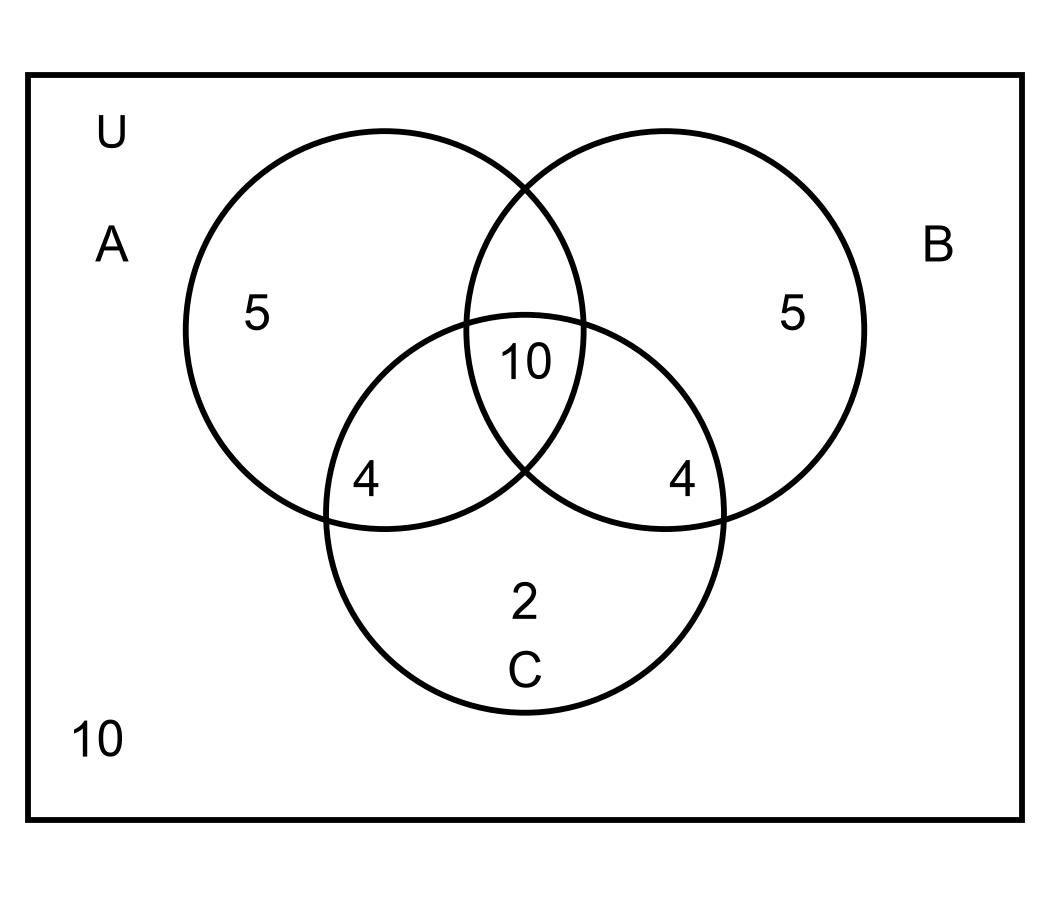
\includegraphics[width=0.38\textwidth]{figures/venn_50_ABC.png}
\end{center}
\step{所以单选物理、化学的人数至多 10 人.}
\step{所以至多选选择物理和化学这两门课程的学生人数至多 $10+10=20$ 人.}
\step{故选 C.}
\solend

\fi

\item 设 $k\geqslant 1,\,k\in\mathbb{N}$，已知集合 $M=\{1,2,3,4,5\}$，若集合 $N_1,N_2,\dots,N_k$ 是集合 $M$ 的 $k$ 个不同非空子集，且 $N_1\cup N_2\cup\dots\cup N_k\neq M$，则 $k$ 的最大值为\mbox{（\quad）.}

\keepwithprev
A. $15$\qquad B. $16$\qquad C. $31$\qquad D. $32$

\ans{A}

\ifanswer
\solbegin
\step{由 $N_1\cup N_2\cup\dots\cup N_k\neq M$ 得所有非空子集的并集缺少集合 $M$ 中至少一个元素.}
\step{假设缺少元素 1，则所有非空子集 $N_i$ 均不含元素 1，即 $N_i$ 是集合 $\{2,3,4,5\}$ 非空子集，集合 $\{2,3,4,5\}$ 的非空子集个数为 $2^4-1=15$，且这些子集 $N_i$ 的并集必不含 1，满足条件.}
\step{假设 $k\geqslant 16$，要满足所有非空子集的并集不等于集合 $M$，必须至少有一个集合 $M$ 中的元素不在任何一个子集中，否则并集就会等于 $M$.}
\step{设这个缺失的元素是 1，那么 $k$ 个非空集都不含元素 1，即每个子集都是集合 $\{2,3,4,5\}$ 的非空子集.}
\step{而集合 $\{2,3,4,5\}$ 只有 $2^4-1=15$ 个不同的非空子集，所以无法从中取出至少 16 个不同的非空子集.}
\step{因此假设不成立，$k$ 必须小于 16.}
\step{所以 $k$ 的最大值为 15，故选 A.}
\solend

\fi

% 注：原卷此题的差集记号是反斜杠 $A\setminus B$（本稿曾误作 $A\vee B$）；$C$ 的集合描述里原卷留了一条
%     待填横线“$x\in A\underline{\quad}B$”（选项按填入的符号分四种情形），本稿曾误作 $\vee\vee$。
%     2026-09-15 回原图核对时已按原卷改回。
\item 对于集合 $A$、$B$，定义 $A\setminus B=\{x\mid x\in A\text{ 且 }x\notin B\}$，则对于集合 $A=\{x\mid x=6n+5,\,n\in\mathbb{N}\}$，$B=\{y\mid y=3m+7,\,m\in\mathbb{N}\}$，$C=\{x\mid x\in A\underline{\hspace{4em}}B\text{ 且 }x<1000\}$，以下说法正确的是\mbox{（\quad）.}

\keepwithprev
A. 若在横线上填入“$\cap$”，则 $C$ 的真子集有 $2^{12}-1$ 个；

B. 若在横线上填入“$\cup$”，则 $C$ 中元素个数大于 250；

C. 若在横线上填入“$\setminus$”，则 $C$ 的非空真子集有 $2^{153}-2$ 个；

% 注：原卷选项 D 作“若在横线上填入“$\cup\complement_{\mathbb N}$”，则 $\complement_{\mathbb N}C$ 中元素个数为 13”；
%     本稿曾把 $\complement_{\mathbb N}$ 抄成 $\varnothing$、把 $\complement_{\mathbb N}C$ 抄成 $C\setminus C$，2026-09-15 回原图核对时已订正。
D. 若在横线上填入“$\cup\complement_{\mathbb{N}}$”，则 $\complement_{\mathbb{N}}C$ 中元素个数为 13.

\ans{B}

\ifanswer
\solbegin
\step{$x=6n+5=3(2n+1)+2$，$y=3m+7=3(m+2)+1$，集合 $A$、$B$ 无公共元素.}
\step{选项 A 中，集合 $C$ 为空集，没有真子集，$A$ 错；}
\step{选项 B 中，由 $6n+5<1000$ 得 $n<165\tfrac{5}{6}$，由 $3m+7<1000$ 得 $m<331$，因此 $C$ 中元素个数为 $166+331=497$，B 正确；}
\step{选项 C 中，$C$ 中元素个数为 166，非空真子集个数为 $2^{166}-2$，C 错；}
% 注：原卷此行作“$\complement_{\mathbb N}C=\complement_{\mathbb N}(A\cup\complement_{\mathbb N}B)
%     =\complement_{\mathbb N}A\cap\complement_{\mathbb N}(\complement_{\mathbb N}B)=\complement_{\mathbb N}A\cap B$，
%     而 $B\subseteq\complement_{\mathbb N}A$”；本稿曾把 $\complement_{\mathbb N}$ 抄成 $C\setminus$，同日已订正。
\step{选项 D 中，$\complement_{\mathbb{N}}C=\complement_{\mathbb{N}}(A\cup\complement_{\mathbb{N}}B)=\complement_{\mathbb{N}}A\cap\complement_{\mathbb{N}}(\complement_{\mathbb{N}}B)=\complement_{\mathbb{N}}A\cap B$，而 $B\subseteq\complement_{\mathbb{N}}A$.}
\step{因此其中元素个数为 331 个，D 错.}
\step{故选 B.}
\solend

\fi
\end{enumerate}

\bigsec{三、解答题}

\begin{enumerate}
\setcounter{enumi}{16}

\item 已知集合 $A=\{x\mid x<-1\text{ 或 }x>4\}$，$B=\{x\mid m+1\leqslant x\leqslant 2m+4\}$.
\begin{enumerate}[label=(\arabic*)]
\item 若 $m=2$，求 $A\cup B$ 和 $\left(\complement_{\R} A\right)\cap B$；
\item 若 $A\cap B=\varnothing$，求 $m$ 的取值范围.
\end{enumerate}

\ans{（1）$A\cup B=\{x\mid x<-1\text{ 或 }x\geqslant 3\}$，$\left(\complement_{\R} A\right)\cap B=\{x\mid 3\leqslant x\leqslant 4\}$；（2）$(-\infty,-3)\cup[-2,0]$}

\ifanswer
\solbegin
\stepm{(1)}{当 $m=2$ 时，集合 $B=\{x\mid 3\leqslant x\leqslant 8\}$.}
\step{又因为 $A=\{x\mid x<-1\text{ 或 }x>4\}$，则 $\complement_{\R}A=\{x\mid -1\leqslant x\leqslant 4\}$，所以 $A\cup B=\{x\mid x<-1\text{ 或 }x\geqslant 3\}$，$\left(\complement_{\R} A\right)\cap B=\{x\mid 3\leqslant x\leqslant 4\}$.}
\stepm{(2)}{因为 $A\cap B=\varnothing$，所以当 $B=\varnothing$ 时，$m+1>2m+4$，解得 $m<-3$ 满足题意；}
\step{当 $B\neq\varnothing$ 时，要满足题意，只需 $\begin{cases}m+1\leqslant 2m+4 \\ m+1\geqslant -1 \\ 2m+4\leqslant 4\end{cases}$，解得 $-2\leqslant m\leqslant 0$.}
\step{综上，实数 $m$ 的范围为 $m<-3$ 或 $-2\leqslant m\leqslant 0$，即 $(-\infty,-3)\cup[-2,0]$.}
\solend

\fi
\ansspace[6]
\item 设集合 $A=\{x\mid x^2+4x=0\}$，$B=\{x\mid x^2+2(a+1)x+a^2-1=0\}$.
\begin{enumerate}[label=(\arabic*)]
\item 写出集合 $A$ 的所有子集；
\item 若 $A\cap B=B$，求实数 $a$ 的取值范围.
\end{enumerate}

\ans{（1）$\{\varnothing,\{0\},\{-4\},\{0,-4\}\}$；（2）$a=1$ 或 $a\leqslant -1$}

\ifanswer
\solbegin
% 注：原卷此行印作“集合 $A$ 的所有子集为 $\varnothing,\{0\},\{-4\},\{0-4\}$”（末项漏逗号、且未加外层花括号）；
%     本稿按规范的列举写法给出，2026-09-15 回原图核对时加注。
\stepm{(1)}{由题意得 $A=\{0,-4\}$，集合 $A$ 的所有子集为 $\varnothing,\{0\},\{-4\},\{0,-4\}$.}
\stepm{(2)}{由 $A\cap B=B$ 得 $B\subseteq A$，所以 $B=\{0\}$ 或 $B=\{-4\}$ 或 $B=\{0,-4\}$ 或 $B=\varnothing$.}
\step{若 $B=\{0\}$ 时，$x^2+2(a+1)x+a^2-1=0$ 有两个相等的根 $0$，则 $\begin{cases}-2(a+1)=0 \\ a^2-1=-4\times(-4)\end{cases}$，解得 $a=-1$.}
\step{若 $B=\{-4\}$ 时，$x^2+2(a+1)x+a^2-1=0$ 有两个相等的根 $-4$，则 $\left\{\begin{matrix}-2(a+1)=-8 \\ a^2-1=-4\times(-4)\end{matrix}\right.$，$a$ 无解.}
\step{若 $B=\{0,-4\}$ 时，$x^2+2(a+1)x+a^2-1=0$ 有两个不相等的根 $0$ 和 $-4$，则 $\begin{cases}-2(a+1)=-4 \\ a^2-1=0\end{cases}$，解得 $a=1$.}
\step{当 $B=\varnothing$ 时，$x^2+2(a+1)x+a^2-1=0$ 无实数根，$\Delta=[2(a+1)]^2-4(a^2-1)=8a+8<0$，得 $a<-1$.}
\step{综上，$a=1$ 或 $a\leqslant -1$.}
\solend

\fi
\ansspace[6]
\item 已知集合 $A=\{x\mid x^2-5x+6=0\}$，$B=\{x\mid mx+1=0\}$，$C=\{x\in\mathbb{N}\mid \sqrt{x}\leqslant 1\}$，且 $A\cup B=A$.
\begin{enumerate}[label=(\arabic*)]
\item 求集合 $M=\{x\mid x\subseteq A\}$ 的真子集的个数；
\item 求实数 $m$ 的值组成的集合；
% 注：原卷本题的定义作“集合 $E=\{x\mid -x\in D,\,2-x^2\notin D\}$”；本稿曾把 $\notin$ 抄成 $\in$
%     （那样 $E=\varnothing$，与答案 $-5$ 冲突），2026-09-15 回原图核对时已订正。
\item 若集合 $D=A\cup C$，定义：集合 $E=\{x\mid -x\in D,\,2-x^2\notin D\}$，求集合 $E$ 中所有元素的和.
\end{enumerate}

\ans{（1）$15$；（2）$\left\{0,-\tfrac{1}{2},-\tfrac{1}{3}\right\}$；（3）$-5$}

\ifanswer
\solbegin
\stepm{(1)}{$A=\{x\mid x^2-5x+6=0\}=\{2,3\}$.}
\step{由 $M=\{x\mid x\subseteq A\}$ 得 $M$ 是 $A$ 的所有子集构成的集合，集合 $A$ 有 2 个元素，故 $A$ 的子集共 $2^2=4$ 个，即 $M$ 含 4 个元素，$M$ 的真子集个数为 $2^4-1=15$.}
\stepm{(2)}{由 (1) 得 $A=\{2,3\}$，集合 $B=\{x\mid mx+1=0\}$.}
\step{由 $A\cup B=A$ 得 $B\subseteq A$，分两种情况：① 当 $m=0$ 时，方程 $mx+1=0$ 无解，$B=\varnothing$，空集是任意集合的子集，符合条件；}
\stepm{②}{当 $m\neq 0$ 时，$B=\{-\tfrac{1}{m}\}$，由 $B\subseteq A$ 得 $-\tfrac{1}{m}=2$ 或 $-\tfrac{1}{m}=3$，解得 $m=-\tfrac{1}{2}$ 或 $m=-\tfrac{1}{3}$.}
\step{实数 $m$ 的取值集合为 $\left\{0,-\tfrac{1}{2},-\tfrac{1}{3}\right\}$.}
\stepm{(3)}{由 (1) 得 $A=\{2,3\}$.}
\step{由 $x\in\mathbb{N}$ 且 $\sqrt{x}\leqslant 1$，得 $x=0$ 或 $x=1$，故 $C=\{0,1\}$.}
\step{所以 $D=A\cup C=\{0,1,2,3\}$.}
\step{由 $-x\in D$ 得 $x$ 的候选值为 $0,-1,-2,-3$.}
\step{由于集合 $E=\{x\mid -x\in D,\,2-x^2\in D\}$，当 $x=0$ 时，$2-x^2=2\in D$，不符合题意；}
\step{当 $x=-1$ 时，$2-x^2=1\in D$，不符合题意；}
\step{当 $x=-2$ 时，$2-x^2=-2\notin D$，符合题意；}
\step{当 $x=-3$ 时，$2-x^2=-7\notin D$，符合题意.}
\step{故 $E=\{-2,-3\}$，所有元素的和为 $-2+(-3)=-5$.}
\solend

\fi
\ansspace[8]
\item 设集合 $M$ 是至少含有两个元素的数集，若 $M$ 中存在两个元素 $x$、$y$ 满足它们的积 $xy\in M$，则称 $M$ 为可积数集.
\begin{enumerate}[label=(\arabic*)]
\item 设集合 $A=\{2,3,5\}$，试判断 $A$ 是否为可积数集？并说明理由；
\item 设集合 $B=\{2,3,4,a\}$，若 $B$ 为可积数集，求实数 $a$ 的取值集合；
\item 设集合 $D=\{x\mid t<x<t+2\}$，若 $D$ 不是可积数集，求实数 $t$ 的取值范围.
\end{enumerate}

% 注：原卷本题【答案】与文末解析的结论都含 $\frac{3}{4}$；本稿曾漏掉 $\frac{3}{4}$
%     （与本稿自己的解析结论不一致），2026-09-15 回原图核对时已订正。
\ans{（1）否；（2）$\left\{0,\tfrac{1}{2},\tfrac{2}{3},\tfrac{3}{4},1,\tfrac{4}{3},\tfrac{3}{2},6,8,12\right\}$；（3）$t\in(-\infty,-2]\cup[2,+\infty)$}

\ifanswer
\solbegin
\stepm{(1)}{因为 $2\times 3=6\notin A$，$2\times 5=10\notin A$，$3\times 5=15\notin A$，所以 $A$ 中任意两个元素的积都不是 $A$ 中的元素，即 $A$ 不是可积数集.}
\stepm{(2)}{若 $B=\{2,3,4,a\}$ 为可积数集，则 $2\times 3=6\in B$，或 $2\times 4=8\in B$ 或 $3\times 4=12\in B$ 或 $2a\in B$ 或 $3a\in B$ 或 $4a\in B$.}
\step{若 $6\in B$，则 $a=6$；}
\step{若 $8\in B$，则 $a=8$；}
\step{若 $12\in B$，则 $a=12$；}
\step{若 $2a\in B$，则 $2a=2$ 或 $2a=3$ 或 $2a=4$ 或 $2a=a$，解得 $a=1$ 或 $a=\tfrac{3}{2}$ 或 $a=2$（舍）或 $a=0$；}
\step{若 $3a\in B$，则 $3a=2$ 或 $3a=3$ 或 $3a=4$ 或 $3a=a$，解得 $a=\tfrac{2}{3}$ 或 $a=1$ 或 $a=\tfrac{4}{3}$ 或 $a=0$；}
\step{若 $4a\in B$，则 $4a=2$ 或 $4a=3$ 或 $4a=4$ 或 $4a=a$，解得 $a=\tfrac{1}{2}$ 或 $a=\tfrac{3}{4}$ 或 $a=1$ 或 $a=0$.}
\step{综上，实数 $a$ 的取值集合为 $\left\{0,\tfrac{1}{2},\tfrac{2}{3},\tfrac{3}{4},1,\tfrac{4}{3},\tfrac{3}{2},6,8,12\right\}$.}
\stepm{(3)}{若 $D=\{x\mid t<x<t+2\}$ 不是可积数集，则 $\forall x,y\in(t,t+2)$，$xy\notin(t,t+2)$.}
\step{当 $t+2\leqslant 0$，即 $t\leqslant -2$ 时，$0\leqslant(t+2)^2<xy<t^2$，此时 $xy\notin D$，满足题意；}
\step{当 $t\geqslant 0$ 时，$0\leqslant t^2<xy<(t+2)^2$，因为 $(t+2)^2>t$，所以若 $xy\notin D$，则 $t^2\geqslant t+2$，即 $t^2-t-2\geqslant 0$，解得 $t\geqslant 2$ 或 $t\leqslant -1$，此时 $t\geqslant 2$ 满足题意；}
% 注：原卷此句作“当 $t<0<t+2$，即 $-2<t<0$ 时，$\exists x=0$，$xy=0\in D$，不满足题意，舍去”；
%     本稿曾把 $\in D$ 抄成 $\notin D$（$-2<t<0$ 时 $0\in(t,t+2)$，确有 $0\in D$），同日已订正。
\step{当 $t<0<t+2$，即 $-2<t<0$ 时，$\exists x=0$，$xy=0\in D$，不满足题意，舍去.}
\step{综上，所求实数 $t$ 的取值范围为 $t\geqslant 2$ 或 $t\leqslant -2$，故 $t\in(-\infty,-2]\cup[2,+\infty)$.}
\solend

\fi
\ansspace[8]
\ansneed{7cm}
\item 已知集合 $A$ 为非空数集，定义：$S=\{x\mid x=a+b,\,a,b\in A\}$，$T=\{x\mid x=|a-b|,a,b\in A\}$（实数 $a$、$b$ 可以相同）.
\begin{enumerate}[label=(\arabic*)]
\item 若集合 $A=\{2,5\}$，直接写出集合 $S$、$T$；
\item 若集合 $A=\{x_1,x_2,x_3,x_4\}$，$x_1<x_2<x_3<x_4$，且 $T=A$，求证：$x_1+x_4=x_3+x_2$；
\item 若集合 $A\subseteq\{x\mid 0\leqslant x\leqslant 2025,\,x\in\mathbb{N}\}$，$S\cap T=\varnothing$，记 $|A|$ 为集合 $A$ 中的元素个数，求 $|A|$ 的最大值.
\end{enumerate}

\ans{（1）$S=\{4,7,10\}$，$T=\{0,3\}$；（2）略；（3）$1350$}

\ifanswer
\solbegin
\stepm{(1)}{$S=\{4,7,10\}$，$T=\{0,3\}$.}
\stepm{(2)}{由集合 $A=\{x_1,x_2,x_3,x_4\}$，$x_1<x_2<x_3<x_4$，则 $T$ 集合的元素在 $0,x_2-x_1,x_3-x_1,x_4-x_1,x_3-x_2,x_4-x_2,x_4-x_3$ 中，且 $0<x_2-x_1<x_3-x_1<x_4-x_1$，$x_3-x_2<x_4-x_2<x_4-x_3$，因为 $A=T$，所以 $A$ 中最大元素 $x_4$ 必在 $T$ 中，而 $x_4-x_1$ 为 7 个元素中的最大者.}
\step{故 $x_4=x_4-x_1$，即 $x_1=0$.}
\step{故 $A=\{0,x_2,x_3,x_4\}$.}
\step{则 $x_3-x_2$、$x_4-x_2$、$x_4-x_3$ 与 $x_2$、$x_3$、$x_4$ 重复.}
\step{而 $0<x_3-x_2<x_3$，故 $x_3-x_2=x_2$，即 $x_3=2x_2$.}
% 注：原卷此句作“而 $0<x_4-x_3<x_4$，故 $x_4-x_3=x_2$ 或 $x_4-x_3=x_3$”；本稿曾把上界写成 $x_3$
%     （那样排除不了 $x_4-x_3=x_3$，与后半句自相矛盾），2026-09-15 回原图核对时已订正。
\step{而 $0<x_4-x_3<x_4$，故 $x_4-x_3=x_2$ 或 $x_4-x_3=x_3$.}
\step{若 $x_4=2x_3=4x_2$，则 $A=\{0,x_2,2x_2,4x_2\}$，$4x_2-x_2=3x_2\notin T$，与题设矛盾.}
\step{故 $x_4-x_3=x_2$，又因为 $x_1=0$，所以 $x_4+x_1=x_3+x_2$.}
% 注：原卷此行作“则 $2a_1<a_1+a_2<a_1+a_3<\cdots<a_1+a_k<a_2+a_k<a_3+a_k<\cdots<a_{k-1}+a_k<2a_k$，
%     所以 $|S|\geqslant 2k-1$，$a_1-a_1<a_2-a_1<a_3-a_1<\cdots<a_k-a_1$，所以 $|T|\geqslant k$”；
%     本稿曾把这个不等式链抄乱（作 $\cdots<a_1+a_k<a_2+a_3<a_k+a_k\leqslant 2a_k$）且把首项写成 $a_i-a_1$，
%     2026-09-15 回原图核对时已订正。
\stepm{(3)}{设 $A=\{a_1,a_2,\dots,a_k\}$ 满足题意，其中 $a_1<a_2<\dots<a_k$，则 $2a_1<a_1+a_2<a_1+a_3<\dots<a_1+a_k<a_2+a_k<a_3+a_k<\dots<a_{k-1}+a_k<2a_k$，所以 $|S|\geqslant 2k-1$，$a_1-a_1<a_2-a_1<a_3-a_1<\dots<a_k-a_1$，所以 $|T|\geqslant k$.}
\step{因为 $S\cap T=\varnothing$，由容斥原理得 $|S\cup T|=|S|+|T|\geqslant 3k-1$.}
\step{$S\cup T$ 中最小的元素为 0，最大的元素为 $2a_k$，$|S\cup T|\leqslant 2a_k+1$，所以 $3k-1\leqslant 2a_k+1\leqslant 2\times 2025+1\,(k\geqslant 1,k\in\mathbb{N})$，即 $3k-1\leqslant 4051$，解得 $k\leqslant 1350\tfrac{2}{3}$.}
\step{实际上 $A=\{676,677,678,\dots,2025\}$ 时满足题意，证明如下：设 $A=\{m,m+1,m+2,\dots,2025\}$，$m\in\mathbb{N}$.}
\step{则 $S=\{2m,2m+1,2m+2,\dots,4050\}$，$T=\{0,1,2,\dots,2025-m\}$.}
\step{由题意得 $2025-m<2m$，即 $m>675$.}
\step{所以 $A=\{676,677,678,\dots,2025\}$ 时满足题意，此时集合 $A$ 中的元素的个数最多.}
\step{综上所述，集合 $A$ 中元素的个数的最大值是 1350.}
\solend

\fi
\ansspace*[10]
\end{enumerate}

\end{document}"
%
% 原始材料是微信公众号图文（“魔都数学加油站”，作者署名“破晓”），正文为 11 张 PNG 页
% （1080×1527）；卷面上的粉色斜水印“魔都数学加油站”属水印，未录入。原文本身就是一份
% **讲评版**——题下直接印出【答案】或【解析】，本稿把这些答案与解析移到答案版，试卷版即
% 一张干净的空卷。
%
% 与原卷的排版差异（均已在 README“说明”中交代）：
%   ① 原文自**第 3 题**起（第 1、2 题未在该文发布），源码里以 \setcounter{enumi}{2} 起编；
%   ② 原卷本就印有分节标题“一、填空题”“二、选择题”“三、解答题”（已在原图上逐页放大
%      核对过），本稿照原卷分节，只把标题改排成全稿统一的“大节标题”样式；
%   ③ 原卷的实数集、整数集符号作正体 $R$（第 7 题）、$Z$（第 11 题），本稿按全稿惯例统一
%      写作 $\R$、$\Z$；
%   ④ 第 14 题【解析】里的 Venn 图取自原卷截图（`figures/venn_50_ABC.png`，4× LANCZOS
%      放大），未用 TikZ 重绘.

\documentclass[a4paper,11pt]{article}
\usepackage{common}

\begin{document}

\examtitlest{2026--2027 学年度交附闵行高一上周练 1}{集合与常用逻辑用语}

\bigsec{一、填空题}

\begin{enumerate}
\setcounter{enumi}{2}

\item 已知集合 $A=\{2,14,x^2+5\}$，$B=\{2,2x\}$，若 $A\cap B=B$，则实数 $x=$ \blankline[2em].

\ans{$7$}

\ifanswer
\solbegin
\step{因为 $A\cap B=B$，所以 $B\subseteq A$，所以 $2x=14$ 或 $x^2+5=2x$.}
\step{$2x=14$ 时，$x=7$，此时 $A=\{2,14,54\}$，$B=\{2,14\}$ 满足题意；}
\step{$x^2+5=2x$ 时，$(x-1)^2+4=0$，无解.}
\step{所以 $x=7$.}
\solend

\fi
\item 设集合 $A=\{y\mid y=x^2-1\}$，$B=\{(x,y)\mid y=x\}$，则 $A\cap B=$ \blankline[2em].

\ans{$\varnothing$}

\item 若集合 $\{0,-1,2a\}=\{a-1,-|a|,a+1\}$，实数 $a$ 的值为 \blankline[2em].

\ans{$\pm 1$}

\ifanswer
\solbegin
\step{令 $A=\{0,-1,2a\}$，$B=\{a-1,-|a|,a+1\}$，因为 $\{0,-1,2a\}=\{a-1,-|a|,a+1\}$，若 $a-1=0$，则 $a=1$，则 $A=\{0,-1,2\}$，$B=\{0,-1,2\}$，满足要求；}
\step{若 $-|a|=0$，则 $a=0$，则 $A=\{0,-1,0\}$，不满足集合元素的互异性；}
\step{若 $a+1=0$，则 $a=-1$，则 $A=\{0,-1,-2\}$，$B=\{0,-1,-2\}$，满足要求.}
\step{故实数 $a$ 的值为 $\pm 1$.}
\solend

\fi
\item 已知全集 $U=(-4,3]$，$A=\{x\in U\mid x^2+2x-8=0\}$，$B=\{x\in U\mid -3<1-2x\leqslant 5\}$，则 $\left(\complement_U B\right)\cap A=$ \blankline[2em].

\ans{$\{2\}$}

\item 已知集合 $A=\{x\mid 1-a\leqslant x\leqslant 1+a,\,a\in\R\}$ 中只有一个整数元素，则实数 $a$ 的取值范围为 \blankline[2em].

\ans{$[0,1)$}

\ifanswer
\solbegin
\step{集合 $A=\{x\mid 1-a\leqslant x\leqslant 1+a,\,a\in\R\}$ 中只有一个整数元素，则 $A\neq\varnothing,\,1-a\leqslant 1+a$，即 $a\geqslant 0$，此时 $1\in A$，故 $\begin{cases}1+a<2 \\ 1-a>0\end{cases}$，解得 $a<1$.}
\step{故 $a\in[0,1)$.}
\solend

\fi
\item 已知全集 $U=\{x\in\mathbb{N}\mid x\leqslant 9\}$，$A\cap B=\{3\}$，$\overline{A}\cap B=\{4,6,8\}$，$A\cap\overline{B}=\{1,5\}$，则 $\overline{A}=$ \blankline[2em].

\ans{$\{0,2,4,6,7,8,9\}$}

\ifanswer
\solbegin
\step{由题意得 $U=\{x\in\mathbb{N}\mid x\leqslant 9\}=\{0,1,2,3,4,5,6,7,8,9\}$，$A\cap B=\{3\}$ 得 $A$、$B$ 中含有元素 $3$；}
\step{$\overline{A}\cap B=\{4,6,8\}$ 得 $B$ 中含有 $4$、$6$、$8$，集合 $A$ 中不含 $4$、$6$、$8$；}
\step{$A\cap\overline{B}=\{1,5\}$ 得 $A$ 含有 $1$、$5$，集合 $B$ 不含 $1$、$5$.}
\step{对于 $0$，假设集合 $A$ 中含有 $0$，由 $A\cap B=\{3\}$ 得 $B$ 不含 $0$，则 $A\cap\overline{B}$ 必含元素 $0$，与 $A\cap\overline{B}=\{1,5\}$ 矛盾.}
\step{同理可得集合 $A$ 中不含元素 $2$、$7$、$9$.}
\step{综上所述，$A=\{1,3,5\}$.}
\step{故 $\overline{A}=\{0,2,4,6,7,8,9\}$.}
\solend

\fi
\item 已知一个有四个数字元素的集合 $S$，$S$ 的所有子集的元素和（空集的元素和认为是 0）的总和为 16208，则 $S$ 的元素之和等于 \blankline[2em].

\ans{$2026$}

\ifanswer
\solbegin
\step{设 $S=\{a_1,a_2,a_3,a_4\}$，$S$ 的每个元素在所有子集中均出现 $2^3$ 次，故 $(a_1+a_2+a_3+a_4)\cdot 2^3=16208$，所以 $a_1+a_2+a_3+a_4=2026$，故 $S$ 的元素之和等于 2026.}
\solend

\fi
\item 已知集合 $M=\{x\in\mathbb{N}\mid 1\leqslant x\leqslant 12\}$，集合 $A_1$、$A_2$、$A_3$ 满足：① 每个集合都恰有 4 个元素；② $A_1\cup A_2\cup A_3=M$. 集合 $A_i\,(i=1,2,3)$ 中元素的最大值与最小值之和称为集合 $A_i$ 的特征数，记为 $X_i\,(i=1,2,3)$，则 $X_1+X_2+X_3$ 的最大值与最小值的积为 \blankline[2em].

\ans{$1485$}

\ifanswer
\solbegin
\step{集合 $M=\{x\in\mathbb{N}\mid 1\leqslant x\leqslant 12\}$ 中最小值为 1，最大值为 12.}
% 注：原卷此处印作“则 $A_1=13$”（原卷笔误，按上下文应为 $X_1=13$），本稿按 $X_1$ 规范，2026-09-15 回原图核对时加注。
\stepm{①}{若使 $X_1+X_2+X_3$ 取得最大值，不妨设 $A_1=\{1,2,3,12\}$，则 $X_1=13$，则剩余的数中最小值是 4，最大值是 11，令 $A_2=\{4,5,6,11\}$，则 $X_2=15$，则 $A_3=\{7,8,9,10\}$，$X_3=17$，则 $X_1+X_2+X_3$ 的最大值为 $13+15+17=45$；}
\stepm{②}{若使 $X_1+X_2+X_3$ 取得最小值，则 $A_1=\{1,4,5,6\}$，则 $X_1=7$，令 $A_2=\{2,7,8,9\}$，则 $X_2=11$，则 $A_3=\{3,10,11,12\}$，$X_3=15$，则此时 $X_1+X_2+X_3$ 的最小值为 $7+11+15=33$.}
\step{故 $X_1+X_2+X_3$ 的最大值与最小值的积为 $45\times 33=1485$.}
\solend

\fi
\item 对于集合 $M=\{a\mid a=x^2-y^2,\,x\in\Z,\,y\in\Z\}$，给出如下三个结论：

① 如果 $P=\{b\mid b=2n+1,\,n\in\Z\}$，那么 $P\subseteq M$；

% 注：原卷此条作“如果 $c=4n+2$，$n\in\Z$，那么 $c\notin M$”；本稿曾把 $\notin$ 抄成 $\in$
%     （那样②为假，与本卷答案 ①②③ 冲突），2026-09-15 回原图核对时已订正。
② 如果 $c=4n+2$，$n\in\Z$，那么 $c\notin M$；

③ 如果 $a_1\in M$，$a_2\in M$，那么 $a_1a_2\in M$. 其中正确结论的序号是 \blankline[2em].

\ans{①②③}

\ifanswer
\solbegin
\stepm{①}{由已知 $b=2n+1,\,n\in\Z$，则恒有 $2n+1=(n+1)^2-n^2,\,n\in\Z$，所以 $2n+1\in M$，所以 $P\subseteq M$，所以①正确；}
\stepm{②}{元素 $c=4n+2,\,n\in\Z$，若 $4n+2\in M$，则存在 $x$、$y\in\Z$ 使得 $x^2-y^2=4n+2$，所以 $4n+2=(x+y)(x-y)$，则 $x+y$ 与 $x-y$ 同奇或同偶.}
\step{若 $x+y$ 与 $x-y$ 都是奇数，则 $(x+y)(x-y)$ 为奇数，而 $4n+2$ 是偶数；}
\step{若 $x+y$ 和 $x-y$ 都是偶数，则 $(x+y)(x-y)$ 能被 4 整除，而 $4n+2$ 不能被 4 整除.}
\step{所以 $4n+2\notin M$，即 $c\notin M$，故②正确；}
\stepm{③}{因为 $a_1$、$a_2\in M$，则 $a_1a_2$ 还是整数，所以 $a_1a_2\in M$，故③正确.}
\step{故正确的是①②③.}
\solend

\fi
\item 用 $C(A)$ 表示非空集合 $A$ 中的元素的个数，定义 $A*B=|C(A)-C(B)|$，若 $A=\{x\mid x^2-2024x-2025=0\}$，$B=\{x\mid (2x^2+ax)(x^2+2ax+6)=0\}$，若 $A*B=1$，则 $a$ 的所有可能取值构成集合 $M$，则 $C(M)=$ \blankline[2em].

\ans{$5$}

\ifanswer
\solbegin
\step{$x^2-2024x-2025=0$ 得 $x=2025$ 或 $x=-1$，即 $C(A)=2$，因为 $A*B=|C(A)-C(B)|=1$，所以 $C(B)=3$ 或 $C(B)=1$.}
\step{方程 $(2x^2+ax)(x^2+2ax+6)=0$ 化为 $x(2x+a)(x^2+2ax+6)=0$.}
\step{当 $a=0$ 时，方程化为 $2x^3(x^2+6)=0$，解得 $x=0$，所以 $B=\{0\}$，$C(B)=1$，符合题意.}
\step{当 $a\neq 0$ 时，方程化为 $x=0$ 或 $x=-\tfrac{a}{2}$ 或 $x^2+2ax+6=0$.}
\step{因为 $0\neq -\tfrac{a}{2}$，$C(B)\neq 1$，故只有 $C(B)=3$.}
\step{故 $x^2+2ax+6=0$ 有两个相等的非零实数根，所以 $\Delta=4a^2-4\times 6=0$，解得 $a=\pm\sqrt{6}$，符合题意.}
\step{当 $x^2+2ax+6=0$ 有两个不相等实根，设 $x_1$、$x_2$，若 $x_1=-\tfrac{a}{2}$，由韦达定理得 $\begin{cases}x_1+x_2=-2a \\ x_1x_2=6\end{cases}$，% 注：原卷作“得 $x_2=-\frac{3a}{2}$”（由 $x_1+x_2=-2a$、$x_1=-\frac{a}{2}$ 得 $x_2=-\frac{3a}{2}$）；
%     本稿曾漏掉负号，2026-09-15 回原图核对时已订正。
得 $x_2=-\tfrac{3a}{2}$，$-\tfrac{a}{2}\cdot(-\tfrac{3a}{2})=\tfrac{3a^2}{4}=6$，解得 $a=\pm 2\sqrt{2}$，符合题意.}
\step{综上所述，$M=\{0,\sqrt{6},-\sqrt{6},2\sqrt{2},-2\sqrt{2}\}$，所以 $C(M)=5$.}
\solend

\fi
\end{enumerate}

\bigsec{二、选择题}

\begin{enumerate}
\setcounter{enumi}{12}

\item 已知集合 $A=\{1,2,3,4,5\}$，$B=\{x\mid \tfrac{x-1}{2}\in\Z,\,x\in A\}$，则集合 $B$ 的真子集个数为\mbox{（\quad）.}

\keepwithprev
A. $3$\qquad B. $5$\qquad C. $7$\qquad D. $15$

\ans{C}

\ifanswer
\solbegin
\step{已知集合 $A=\{1,2,3,4,5\}$，$B=\{x\mid\tfrac{x-1}{2}\in\Z,\,x\in A\}$.}
\step{因为 $\tfrac{x-1}{2}\in\Z$，所以 $x$ 为奇数，所以 $B=\{1,3,5\}$.}
\step{所以集合 $B$ 中有 3 个元素，所以集合 $B$ 的真子集个数为 $2^3-1=7$.}
\step{故选 C.}
\solend

\fi

\item 高一二班共有学生 50 人，每名学生要从物理、化学、生物、历史、地理、政治这六门课程中选择三门课程进行学习. 已知选择物理、化学、生物的学生各有至少 20 人，这三门课程都不选的有 10 人，这三门课程都选的有 10 人，在这三门课程中选择任意两门课程的都至少有 14 人，物理、化学只选一科的学生都至少 5 人，那么选择物理和化学这两门课程的学生人数至多\mbox{（\quad）.}

\keepwithprev
A. $18$\qquad B. $19$\qquad C. $20$\qquad D. $21$

\ans{C}

\ifanswer
\solbegin
\step{可以把学生 50 人看作一个集合 $U$，选择物理的人数组成集合 $A$，选择化学的人数组成集合 $B$，选择生物的人数组成集合 $C$.}
\step{要使选择物理和化学这两门课程的学生人数最多，除这三门课程都不选的有 10 人，这三门课程都选的有 10 人，则其他科选择人数均为最少，因为物理、化学只选一科的学生都至少 5 人，即得到单选物理的最少 5 人，单选化学的最少 5 人.}
\step{因为在这三门课程中选择任意两门课程的都至少有 14 人，单选化学、生物的最少 4 人，单选物理、生物的最少 4 人.}
\step{因为选择物理、化学、生物的学生各有至少 20 人，所以单选生物的最少 2 人.}
\step{以上人数最少 30 人，可作出如图所示的韦恩图：}
% 注：原卷此处印有一张韦恩图（三个圆 $A$、$B$、$C$，$A$ 独有 5、$B$ 独有 5、三集合公共 10、
%     $A\cap C$ 独有 4、$B\cap C$ 独有 4、$C$ 独有 2、三集合之外 10）；本稿此前漏排此图而正文仍作
%     “如图”，2026-09-15 回原图核对时按原卷截图补入（见 figures/venn_50_ABC.png）。
\begin{center}
% 插图取自原卷截图（裁去截图残影后 4× LANCZOS 放大），不用 TikZ 手绘
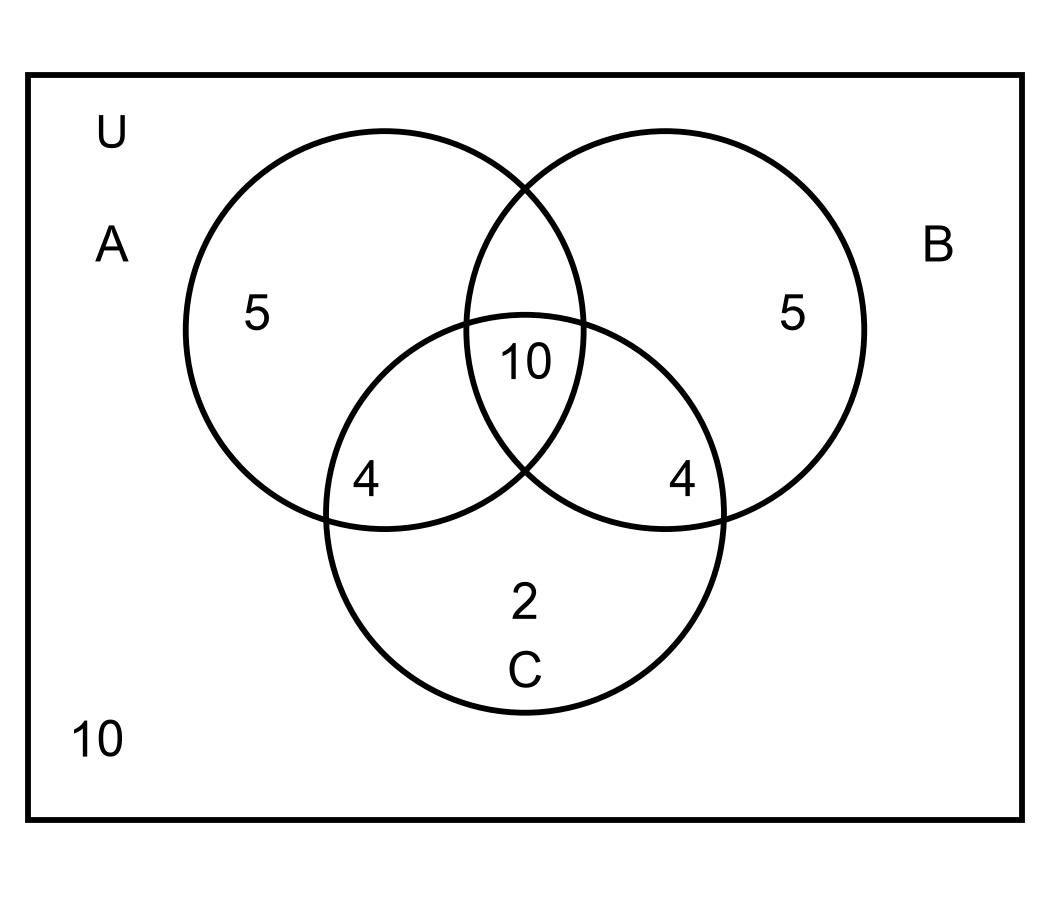
\includegraphics[width=0.38\textwidth]{figures/venn_50_ABC.png}
\end{center}
\step{所以单选物理、化学的人数至多 10 人.}
\step{所以至多选选择物理和化学这两门课程的学生人数至多 $10+10=20$ 人.}
\step{故选 C.}
\solend

\fi

\item 设 $k\geqslant 1,\,k\in\mathbb{N}$，已知集合 $M=\{1,2,3,4,5\}$，若集合 $N_1,N_2,\dots,N_k$ 是集合 $M$ 的 $k$ 个不同非空子集，且 $N_1\cup N_2\cup\dots\cup N_k\neq M$，则 $k$ 的最大值为\mbox{（\quad）.}

\keepwithprev
A. $15$\qquad B. $16$\qquad C. $31$\qquad D. $32$

\ans{A}

\ifanswer
\solbegin
\step{由 $N_1\cup N_2\cup\dots\cup N_k\neq M$ 得所有非空子集的并集缺少集合 $M$ 中至少一个元素.}
\step{假设缺少元素 1，则所有非空子集 $N_i$ 均不含元素 1，即 $N_i$ 是集合 $\{2,3,4,5\}$ 非空子集，集合 $\{2,3,4,5\}$ 的非空子集个数为 $2^4-1=15$，且这些子集 $N_i$ 的并集必不含 1，满足条件.}
\step{假设 $k\geqslant 16$，要满足所有非空子集的并集不等于集合 $M$，必须至少有一个集合 $M$ 中的元素不在任何一个子集中，否则并集就会等于 $M$.}
\step{设这个缺失的元素是 1，那么 $k$ 个非空集都不含元素 1，即每个子集都是集合 $\{2,3,4,5\}$ 的非空子集.}
\step{而集合 $\{2,3,4,5\}$ 只有 $2^4-1=15$ 个不同的非空子集，所以无法从中取出至少 16 个不同的非空子集.}
\step{因此假设不成立，$k$ 必须小于 16.}
\step{所以 $k$ 的最大值为 15，故选 A.}
\solend

\fi

% 注：原卷此题的差集记号是反斜杠 $A\setminus B$（本稿曾误作 $A\vee B$）；$C$ 的集合描述里原卷留了一条
%     待填横线“$x\in A\underline{\quad}B$”（选项按填入的符号分四种情形），本稿曾误作 $\vee\vee$。
%     2026-09-15 回原图核对时已按原卷改回。
\item 对于集合 $A$、$B$，定义 $A\setminus B=\{x\mid x\in A\text{ 且 }x\notin B\}$，则对于集合 $A=\{x\mid x=6n+5,\,n\in\mathbb{N}\}$，$B=\{y\mid y=3m+7,\,m\in\mathbb{N}\}$，$C=\{x\mid x\in A\underline{\hspace{4em}}B\text{ 且 }x<1000\}$，以下说法正确的是\mbox{（\quad）.}

\keepwithprev
A. 若在横线上填入“$\cap$”，则 $C$ 的真子集有 $2^{12}-1$ 个；

B. 若在横线上填入“$\cup$”，则 $C$ 中元素个数大于 250；

C. 若在横线上填入“$\setminus$”，则 $C$ 的非空真子集有 $2^{153}-2$ 个；

% 注：原卷选项 D 作“若在横线上填入“$\cup\complement_{\mathbb N}$”，则 $\complement_{\mathbb N}C$ 中元素个数为 13”；
%     本稿曾把 $\complement_{\mathbb N}$ 抄成 $\varnothing$、把 $\complement_{\mathbb N}C$ 抄成 $C\setminus C$，2026-09-15 回原图核对时已订正。
D. 若在横线上填入“$\cup\complement_{\mathbb{N}}$”，则 $\complement_{\mathbb{N}}C$ 中元素个数为 13.

\ans{B}

\ifanswer
\solbegin
\step{$x=6n+5=3(2n+1)+2$，$y=3m+7=3(m+2)+1$，集合 $A$、$B$ 无公共元素.}
\step{选项 A 中，集合 $C$ 为空集，没有真子集，$A$ 错；}
\step{选项 B 中，由 $6n+5<1000$ 得 $n<165\tfrac{5}{6}$，由 $3m+7<1000$ 得 $m<331$，因此 $C$ 中元素个数为 $166+331=497$，B 正确；}
\step{选项 C 中，$C$ 中元素个数为 166，非空真子集个数为 $2^{166}-2$，C 错；}
% 注：原卷此行作“$\complement_{\mathbb N}C=\complement_{\mathbb N}(A\cup\complement_{\mathbb N}B)
%     =\complement_{\mathbb N}A\cap\complement_{\mathbb N}(\complement_{\mathbb N}B)=\complement_{\mathbb N}A\cap B$，
%     而 $B\subseteq\complement_{\mathbb N}A$”；本稿曾把 $\complement_{\mathbb N}$ 抄成 $C\setminus$，同日已订正。
\step{选项 D 中，$\complement_{\mathbb{N}}C=\complement_{\mathbb{N}}(A\cup\complement_{\mathbb{N}}B)=\complement_{\mathbb{N}}A\cap\complement_{\mathbb{N}}(\complement_{\mathbb{N}}B)=\complement_{\mathbb{N}}A\cap B$，而 $B\subseteq\complement_{\mathbb{N}}A$.}
\step{因此其中元素个数为 331 个，D 错.}
\step{故选 B.}
\solend

\fi
\end{enumerate}

\bigsec{三、解答题}

\begin{enumerate}
\setcounter{enumi}{16}

\item 已知集合 $A=\{x\mid x<-1\text{ 或 }x>4\}$，$B=\{x\mid m+1\leqslant x\leqslant 2m+4\}$.
\begin{enumerate}[label=(\arabic*)]
\item 若 $m=2$，求 $A\cup B$ 和 $\left(\complement_{\R} A\right)\cap B$；
\item 若 $A\cap B=\varnothing$，求 $m$ 的取值范围.
\end{enumerate}

\ans{（1）$A\cup B=\{x\mid x<-1\text{ 或 }x\geqslant 3\}$，$\left(\complement_{\R} A\right)\cap B=\{x\mid 3\leqslant x\leqslant 4\}$；（2）$(-\infty,-3)\cup[-2,0]$}

\ifanswer
\solbegin
\stepm{(1)}{当 $m=2$ 时，集合 $B=\{x\mid 3\leqslant x\leqslant 8\}$.}
\step{又因为 $A=\{x\mid x<-1\text{ 或 }x>4\}$，则 $\complement_{\R}A=\{x\mid -1\leqslant x\leqslant 4\}$，所以 $A\cup B=\{x\mid x<-1\text{ 或 }x\geqslant 3\}$，$\left(\complement_{\R} A\right)\cap B=\{x\mid 3\leqslant x\leqslant 4\}$.}
\stepm{(2)}{因为 $A\cap B=\varnothing$，所以当 $B=\varnothing$ 时，$m+1>2m+4$，解得 $m<-3$ 满足题意；}
\step{当 $B\neq\varnothing$ 时，要满足题意，只需 $\begin{cases}m+1\leqslant 2m+4 \\ m+1\geqslant -1 \\ 2m+4\leqslant 4\end{cases}$，解得 $-2\leqslant m\leqslant 0$.}
\step{综上，实数 $m$ 的范围为 $m<-3$ 或 $-2\leqslant m\leqslant 0$，即 $(-\infty,-3)\cup[-2,0]$.}
\solend

\fi
\ansspace[6]
\item 设集合 $A=\{x\mid x^2+4x=0\}$，$B=\{x\mid x^2+2(a+1)x+a^2-1=0\}$.
\begin{enumerate}[label=(\arabic*)]
\item 写出集合 $A$ 的所有子集；
\item 若 $A\cap B=B$，求实数 $a$ 的取值范围.
\end{enumerate}

\ans{（1）$\{\varnothing,\{0\},\{-4\},\{0,-4\}\}$；（2）$a=1$ 或 $a\leqslant -1$}

\ifanswer
\solbegin
% 注：原卷此行印作“集合 $A$ 的所有子集为 $\varnothing,\{0\},\{-4\},\{0-4\}$”（末项漏逗号、且未加外层花括号）；
%     本稿按规范的列举写法给出，2026-09-15 回原图核对时加注。
\stepm{(1)}{由题意得 $A=\{0,-4\}$，集合 $A$ 的所有子集为 $\varnothing,\{0\},\{-4\},\{0,-4\}$.}
\stepm{(2)}{由 $A\cap B=B$ 得 $B\subseteq A$，所以 $B=\{0\}$ 或 $B=\{-4\}$ 或 $B=\{0,-4\}$ 或 $B=\varnothing$.}
\step{若 $B=\{0\}$ 时，$x^2+2(a+1)x+a^2-1=0$ 有两个相等的根 $0$，则 $\begin{cases}-2(a+1)=0 \\ a^2-1=-4\times(-4)\end{cases}$，解得 $a=-1$.}
\step{若 $B=\{-4\}$ 时，$x^2+2(a+1)x+a^2-1=0$ 有两个相等的根 $-4$，则 $\left\{\begin{matrix}-2(a+1)=-8 \\ a^2-1=-4\times(-4)\end{matrix}\right.$，$a$ 无解.}
\step{若 $B=\{0,-4\}$ 时，$x^2+2(a+1)x+a^2-1=0$ 有两个不相等的根 $0$ 和 $-4$，则 $\begin{cases}-2(a+1)=-4 \\ a^2-1=0\end{cases}$，解得 $a=1$.}
\step{当 $B=\varnothing$ 时，$x^2+2(a+1)x+a^2-1=0$ 无实数根，$\Delta=[2(a+1)]^2-4(a^2-1)=8a+8<0$，得 $a<-1$.}
\step{综上，$a=1$ 或 $a\leqslant -1$.}
\solend

\fi
\ansspace[6]
\item 已知集合 $A=\{x\mid x^2-5x+6=0\}$，$B=\{x\mid mx+1=0\}$，$C=\{x\in\mathbb{N}\mid \sqrt{x}\leqslant 1\}$，且 $A\cup B=A$.
\begin{enumerate}[label=(\arabic*)]
\item 求集合 $M=\{x\mid x\subseteq A\}$ 的真子集的个数；
\item 求实数 $m$ 的值组成的集合；
% 注：原卷本题的定义作“集合 $E=\{x\mid -x\in D,\,2-x^2\notin D\}$”；本稿曾把 $\notin$ 抄成 $\in$
%     （那样 $E=\varnothing$，与答案 $-5$ 冲突），2026-09-15 回原图核对时已订正。
\item 若集合 $D=A\cup C$，定义：集合 $E=\{x\mid -x\in D,\,2-x^2\notin D\}$，求集合 $E$ 中所有元素的和.
\end{enumerate}

\ans{（1）$15$；（2）$\left\{0,-\tfrac{1}{2},-\tfrac{1}{3}\right\}$；（3）$-5$}

\ifanswer
\solbegin
\stepm{(1)}{$A=\{x\mid x^2-5x+6=0\}=\{2,3\}$.}
\step{由 $M=\{x\mid x\subseteq A\}$ 得 $M$ 是 $A$ 的所有子集构成的集合，集合 $A$ 有 2 个元素，故 $A$ 的子集共 $2^2=4$ 个，即 $M$ 含 4 个元素，$M$ 的真子集个数为 $2^4-1=15$.}
\stepm{(2)}{由 (1) 得 $A=\{2,3\}$，集合 $B=\{x\mid mx+1=0\}$.}
\step{由 $A\cup B=A$ 得 $B\subseteq A$，分两种情况：① 当 $m=0$ 时，方程 $mx+1=0$ 无解，$B=\varnothing$，空集是任意集合的子集，符合条件；}
\stepm{②}{当 $m\neq 0$ 时，$B=\{-\tfrac{1}{m}\}$，由 $B\subseteq A$ 得 $-\tfrac{1}{m}=2$ 或 $-\tfrac{1}{m}=3$，解得 $m=-\tfrac{1}{2}$ 或 $m=-\tfrac{1}{3}$.}
\step{实数 $m$ 的取值集合为 $\left\{0,-\tfrac{1}{2},-\tfrac{1}{3}\right\}$.}
\stepm{(3)}{由 (1) 得 $A=\{2,3\}$.}
\step{由 $x\in\mathbb{N}$ 且 $\sqrt{x}\leqslant 1$，得 $x=0$ 或 $x=1$，故 $C=\{0,1\}$.}
\step{所以 $D=A\cup C=\{0,1,2,3\}$.}
\step{由 $-x\in D$ 得 $x$ 的候选值为 $0,-1,-2,-3$.}
\step{由于集合 $E=\{x\mid -x\in D,\,2-x^2\in D\}$，当 $x=0$ 时，$2-x^2=2\in D$，不符合题意；}
\step{当 $x=-1$ 时，$2-x^2=1\in D$，不符合题意；}
\step{当 $x=-2$ 时，$2-x^2=-2\notin D$，符合题意；}
\step{当 $x=-3$ 时，$2-x^2=-7\notin D$，符合题意.}
\step{故 $E=\{-2,-3\}$，所有元素的和为 $-2+(-3)=-5$.}
\solend

\fi
\ansspace[8]
\item 设集合 $M$ 是至少含有两个元素的数集，若 $M$ 中存在两个元素 $x$、$y$ 满足它们的积 $xy\in M$，则称 $M$ 为可积数集.
\begin{enumerate}[label=(\arabic*)]
\item 设集合 $A=\{2,3,5\}$，试判断 $A$ 是否为可积数集？并说明理由；
\item 设集合 $B=\{2,3,4,a\}$，若 $B$ 为可积数集，求实数 $a$ 的取值集合；
\item 设集合 $D=\{x\mid t<x<t+2\}$，若 $D$ 不是可积数集，求实数 $t$ 的取值范围.
\end{enumerate}

% 注：原卷本题【答案】与文末解析的结论都含 $\frac{3}{4}$；本稿曾漏掉 $\frac{3}{4}$
%     （与本稿自己的解析结论不一致），2026-09-15 回原图核对时已订正。
\ans{（1）否；（2）$\left\{0,\tfrac{1}{2},\tfrac{2}{3},\tfrac{3}{4},1,\tfrac{4}{3},\tfrac{3}{2},6,8,12\right\}$；（3）$t\in(-\infty,-2]\cup[2,+\infty)$}

\ifanswer
\solbegin
\stepm{(1)}{因为 $2\times 3=6\notin A$，$2\times 5=10\notin A$，$3\times 5=15\notin A$，所以 $A$ 中任意两个元素的积都不是 $A$ 中的元素，即 $A$ 不是可积数集.}
\stepm{(2)}{若 $B=\{2,3,4,a\}$ 为可积数集，则 $2\times 3=6\in B$，或 $2\times 4=8\in B$ 或 $3\times 4=12\in B$ 或 $2a\in B$ 或 $3a\in B$ 或 $4a\in B$.}
\step{若 $6\in B$，则 $a=6$；}
\step{若 $8\in B$，则 $a=8$；}
\step{若 $12\in B$，则 $a=12$；}
\step{若 $2a\in B$，则 $2a=2$ 或 $2a=3$ 或 $2a=4$ 或 $2a=a$，解得 $a=1$ 或 $a=\tfrac{3}{2}$ 或 $a=2$（舍）或 $a=0$；}
\step{若 $3a\in B$，则 $3a=2$ 或 $3a=3$ 或 $3a=4$ 或 $3a=a$，解得 $a=\tfrac{2}{3}$ 或 $a=1$ 或 $a=\tfrac{4}{3}$ 或 $a=0$；}
\step{若 $4a\in B$，则 $4a=2$ 或 $4a=3$ 或 $4a=4$ 或 $4a=a$，解得 $a=\tfrac{1}{2}$ 或 $a=\tfrac{3}{4}$ 或 $a=1$ 或 $a=0$.}
\step{综上，实数 $a$ 的取值集合为 $\left\{0,\tfrac{1}{2},\tfrac{2}{3},\tfrac{3}{4},1,\tfrac{4}{3},\tfrac{3}{2},6,8,12\right\}$.}
\stepm{(3)}{若 $D=\{x\mid t<x<t+2\}$ 不是可积数集，则 $\forall x,y\in(t,t+2)$，$xy\notin(t,t+2)$.}
\step{当 $t+2\leqslant 0$，即 $t\leqslant -2$ 时，$0\leqslant(t+2)^2<xy<t^2$，此时 $xy\notin D$，满足题意；}
\step{当 $t\geqslant 0$ 时，$0\leqslant t^2<xy<(t+2)^2$，因为 $(t+2)^2>t$，所以若 $xy\notin D$，则 $t^2\geqslant t+2$，即 $t^2-t-2\geqslant 0$，解得 $t\geqslant 2$ 或 $t\leqslant -1$，此时 $t\geqslant 2$ 满足题意；}
% 注：原卷此句作“当 $t<0<t+2$，即 $-2<t<0$ 时，$\exists x=0$，$xy=0\in D$，不满足题意，舍去”；
%     本稿曾把 $\in D$ 抄成 $\notin D$（$-2<t<0$ 时 $0\in(t,t+2)$，确有 $0\in D$），同日已订正。
\step{当 $t<0<t+2$，即 $-2<t<0$ 时，$\exists x=0$，$xy=0\in D$，不满足题意，舍去.}
\step{综上，所求实数 $t$ 的取值范围为 $t\geqslant 2$ 或 $t\leqslant -2$，故 $t\in(-\infty,-2]\cup[2,+\infty)$.}
\solend

\fi
\ansspace[8]
\ansneed{7cm}
\item 已知集合 $A$ 为非空数集，定义：$S=\{x\mid x=a+b,\,a,b\in A\}$，$T=\{x\mid x=|a-b|,a,b\in A\}$（实数 $a$、$b$ 可以相同）.
\begin{enumerate}[label=(\arabic*)]
\item 若集合 $A=\{2,5\}$，直接写出集合 $S$、$T$；
\item 若集合 $A=\{x_1,x_2,x_3,x_4\}$，$x_1<x_2<x_3<x_4$，且 $T=A$，求证：$x_1+x_4=x_3+x_2$；
\item 若集合 $A\subseteq\{x\mid 0\leqslant x\leqslant 2025,\,x\in\mathbb{N}\}$，$S\cap T=\varnothing$，记 $|A|$ 为集合 $A$ 中的元素个数，求 $|A|$ 的最大值.
\end{enumerate}

\ans{（1）$S=\{4,7,10\}$，$T=\{0,3\}$；（2）略；（3）$1350$}

\ifanswer
\solbegin
\stepm{(1)}{$S=\{4,7,10\}$，$T=\{0,3\}$.}
\stepm{(2)}{由集合 $A=\{x_1,x_2,x_3,x_4\}$，$x_1<x_2<x_3<x_4$，则 $T$ 集合的元素在 $0,x_2-x_1,x_3-x_1,x_4-x_1,x_3-x_2,x_4-x_2,x_4-x_3$ 中，且 $0<x_2-x_1<x_3-x_1<x_4-x_1$，$x_3-x_2<x_4-x_2<x_4-x_3$，因为 $A=T$，所以 $A$ 中最大元素 $x_4$ 必在 $T$ 中，而 $x_4-x_1$ 为 7 个元素中的最大者.}
\step{故 $x_4=x_4-x_1$，即 $x_1=0$.}
\step{故 $A=\{0,x_2,x_3,x_4\}$.}
\step{则 $x_3-x_2$、$x_4-x_2$、$x_4-x_3$ 与 $x_2$、$x_3$、$x_4$ 重复.}
\step{而 $0<x_3-x_2<x_3$，故 $x_3-x_2=x_2$，即 $x_3=2x_2$.}
% 注：原卷此句作“而 $0<x_4-x_3<x_4$，故 $x_4-x_3=x_2$ 或 $x_4-x_3=x_3$”；本稿曾把上界写成 $x_3$
%     （那样排除不了 $x_4-x_3=x_3$，与后半句自相矛盾），2026-09-15 回原图核对时已订正。
\step{而 $0<x_4-x_3<x_4$，故 $x_4-x_3=x_2$ 或 $x_4-x_3=x_3$.}
\step{若 $x_4=2x_3=4x_2$，则 $A=\{0,x_2,2x_2,4x_2\}$，$4x_2-x_2=3x_2\notin T$，与题设矛盾.}
\step{故 $x_4-x_3=x_2$，又因为 $x_1=0$，所以 $x_4+x_1=x_3+x_2$.}
% 注：原卷此行作“则 $2a_1<a_1+a_2<a_1+a_3<\cdots<a_1+a_k<a_2+a_k<a_3+a_k<\cdots<a_{k-1}+a_k<2a_k$，
%     所以 $|S|\geqslant 2k-1$，$a_1-a_1<a_2-a_1<a_3-a_1<\cdots<a_k-a_1$，所以 $|T|\geqslant k$”；
%     本稿曾把这个不等式链抄乱（作 $\cdots<a_1+a_k<a_2+a_3<a_k+a_k\leqslant 2a_k$）且把首项写成 $a_i-a_1$，
%     2026-09-15 回原图核对时已订正。
\stepm{(3)}{设 $A=\{a_1,a_2,\dots,a_k\}$ 满足题意，其中 $a_1<a_2<\dots<a_k$，则 $2a_1<a_1+a_2<a_1+a_3<\dots<a_1+a_k<a_2+a_k<a_3+a_k<\dots<a_{k-1}+a_k<2a_k$，所以 $|S|\geqslant 2k-1$，$a_1-a_1<a_2-a_1<a_3-a_1<\dots<a_k-a_1$，所以 $|T|\geqslant k$.}
\step{因为 $S\cap T=\varnothing$，由容斥原理得 $|S\cup T|=|S|+|T|\geqslant 3k-1$.}
\step{$S\cup T$ 中最小的元素为 0，最大的元素为 $2a_k$，$|S\cup T|\leqslant 2a_k+1$，所以 $3k-1\leqslant 2a_k+1\leqslant 2\times 2025+1\,(k\geqslant 1,k\in\mathbb{N})$，即 $3k-1\leqslant 4051$，解得 $k\leqslant 1350\tfrac{2}{3}$.}
\step{实际上 $A=\{676,677,678,\dots,2025\}$ 时满足题意，证明如下：设 $A=\{m,m+1,m+2,\dots,2025\}$，$m\in\mathbb{N}$.}
\step{则 $S=\{2m,2m+1,2m+2,\dots,4050\}$，$T=\{0,1,2,\dots,2025-m\}$.}
\step{由题意得 $2025-m<2m$，即 $m>675$.}
\step{所以 $A=\{676,677,678,\dots,2025\}$ 时满足题意，此时集合 $A$ 中的元素的个数最多.}
\step{综上所述，集合 $A$ 中元素的个数的最大值是 1350.}
\solend

\fi
\ansspace*[10]
\end{enumerate}

\end{document}"
%
% 原始材料是微信公众号图文（“魔都数学加油站”，作者署名“破晓”），正文为 11 张 PNG 页
% （1080×1527）；卷面上的粉色斜水印“魔都数学加油站”属水印，未录入。原文本身就是一份
% **讲评版**——题下直接印出【答案】或【解析】，本稿把这些答案与解析移到答案版，试卷版即
% 一张干净的空卷。
%
% 与原卷的排版差异（均已在 README“说明”中交代）：
%   ① 原文自**第 3 题**起（第 1、2 题未在该文发布），源码里以 \setcounter{enumi}{2} 起编；
%   ② 原卷本就印有分节标题“一、填空题”“二、选择题”“三、解答题”（已在原图上逐页放大
%      核对过），本稿照原卷分节，只把标题改排成全稿统一的“大节标题”样式；
%   ③ 原卷的实数集、整数集符号作正体 $R$（第 7 题）、$Z$（第 11 题），本稿按全稿惯例统一
%      写作 $\R$、$\Z$；
%   ④ 第 14 题【解析】里的 Venn 图取自原卷截图（`figures/venn_50_ABC.png`，4× LANCZOS
%      放大），未用 TikZ 重绘.

\documentclass[a4paper,11pt]{article}
\usepackage{common}

\begin{document}

\examtitlest{2026--2027 学年度交附闵行高一上周练 1}{集合与常用逻辑用语}

\bigsec{一、填空题}

\begin{enumerate}
\setcounter{enumi}{2}

\item 已知集合 $A=\{2,14,x^2+5\}$，$B=\{2,2x\}$，若 $A\cap B=B$，则实数 $x=$ \blankline[2em].

\ans{$7$}

\ifanswer
\solbegin
\step{因为 $A\cap B=B$，所以 $B\subseteq A$，所以 $2x=14$ 或 $x^2+5=2x$.}
\step{$2x=14$ 时，$x=7$，此时 $A=\{2,14,54\}$，$B=\{2,14\}$ 满足题意；}
\step{$x^2+5=2x$ 时，$(x-1)^2+4=0$，无解.}
\step{所以 $x=7$.}
\solend

\fi
\item 设集合 $A=\{y\mid y=x^2-1\}$，$B=\{(x,y)\mid y=x\}$，则 $A\cap B=$ \blankline[2em].

\ans{$\varnothing$}

\item 若集合 $\{0,-1,2a\}=\{a-1,-|a|,a+1\}$，实数 $a$ 的值为 \blankline[2em].

\ans{$\pm 1$}

\ifanswer
\solbegin
\step{令 $A=\{0,-1,2a\}$，$B=\{a-1,-|a|,a+1\}$，因为 $\{0,-1,2a\}=\{a-1,-|a|,a+1\}$，若 $a-1=0$，则 $a=1$，则 $A=\{0,-1,2\}$，$B=\{0,-1,2\}$，满足要求；}
\step{若 $-|a|=0$，则 $a=0$，则 $A=\{0,-1,0\}$，不满足集合元素的互异性；}
\step{若 $a+1=0$，则 $a=-1$，则 $A=\{0,-1,-2\}$，$B=\{0,-1,-2\}$，满足要求.}
\step{故实数 $a$ 的值为 $\pm 1$.}
\solend

\fi
\item 已知全集 $U=(-4,3]$，$A=\{x\in U\mid x^2+2x-8=0\}$，$B=\{x\in U\mid -3<1-2x\leqslant 5\}$，则 $\left(\complement_U B\right)\cap A=$ \blankline[2em].

\ans{$\{2\}$}

\item 已知集合 $A=\{x\mid 1-a\leqslant x\leqslant 1+a,\,a\in\R\}$ 中只有一个整数元素，则实数 $a$ 的取值范围为 \blankline[2em].

\ans{$[0,1)$}

\ifanswer
\solbegin
\step{集合 $A=\{x\mid 1-a\leqslant x\leqslant 1+a,\,a\in\R\}$ 中只有一个整数元素，则 $A\neq\varnothing,\,1-a\leqslant 1+a$，即 $a\geqslant 0$，此时 $1\in A$，故 $\begin{cases}1+a<2 \\ 1-a>0\end{cases}$，解得 $a<1$.}
\step{故 $a\in[0,1)$.}
\solend

\fi
\item 已知全集 $U=\{x\in\mathbb{N}\mid x\leqslant 9\}$，$A\cap B=\{3\}$，$\overline{A}\cap B=\{4,6,8\}$，$A\cap\overline{B}=\{1,5\}$，则 $\overline{A}=$ \blankline[2em].

\ans{$\{0,2,4,6,7,8,9\}$}

\ifanswer
\solbegin
\step{由题意得 $U=\{x\in\mathbb{N}\mid x\leqslant 9\}=\{0,1,2,3,4,5,6,7,8,9\}$，$A\cap B=\{3\}$ 得 $A$、$B$ 中含有元素 $3$；}
\step{$\overline{A}\cap B=\{4,6,8\}$ 得 $B$ 中含有 $4$、$6$、$8$，集合 $A$ 中不含 $4$、$6$、$8$；}
\step{$A\cap\overline{B}=\{1,5\}$ 得 $A$ 含有 $1$、$5$，集合 $B$ 不含 $1$、$5$.}
\step{对于 $0$，假设集合 $A$ 中含有 $0$，由 $A\cap B=\{3\}$ 得 $B$ 不含 $0$，则 $A\cap\overline{B}$ 必含元素 $0$，与 $A\cap\overline{B}=\{1,5\}$ 矛盾.}
\step{同理可得集合 $A$ 中不含元素 $2$、$7$、$9$.}
\step{综上所述，$A=\{1,3,5\}$.}
\step{故 $\overline{A}=\{0,2,4,6,7,8,9\}$.}
\solend

\fi
\item 已知一个有四个数字元素的集合 $S$，$S$ 的所有子集的元素和（空集的元素和认为是 0）的总和为 16208，则 $S$ 的元素之和等于 \blankline[2em].

\ans{$2026$}

\ifanswer
\solbegin
\step{设 $S=\{a_1,a_2,a_3,a_4\}$，$S$ 的每个元素在所有子集中均出现 $2^3$ 次，故 $(a_1+a_2+a_3+a_4)\cdot 2^3=16208$，所以 $a_1+a_2+a_3+a_4=2026$，故 $S$ 的元素之和等于 2026.}
\solend

\fi
\item 已知集合 $M=\{x\in\mathbb{N}\mid 1\leqslant x\leqslant 12\}$，集合 $A_1$、$A_2$、$A_3$ 满足：① 每个集合都恰有 4 个元素；② $A_1\cup A_2\cup A_3=M$. 集合 $A_i\,(i=1,2,3)$ 中元素的最大值与最小值之和称为集合 $A_i$ 的特征数，记为 $X_i\,(i=1,2,3)$，则 $X_1+X_2+X_3$ 的最大值与最小值的积为 \blankline[2em].

\ans{$1485$}

\ifanswer
\solbegin
\step{集合 $M=\{x\in\mathbb{N}\mid 1\leqslant x\leqslant 12\}$ 中最小值为 1，最大值为 12.}
% 注：原卷此处印作“则 $A_1=13$”（原卷笔误，按上下文应为 $X_1=13$），本稿按 $X_1$ 规范，2026-09-15 回原图核对时加注。
\stepm{①}{若使 $X_1+X_2+X_3$ 取得最大值，不妨设 $A_1=\{1,2,3,12\}$，则 $X_1=13$，则剩余的数中最小值是 4，最大值是 11，令 $A_2=\{4,5,6,11\}$，则 $X_2=15$，则 $A_3=\{7,8,9,10\}$，$X_3=17$，则 $X_1+X_2+X_3$ 的最大值为 $13+15+17=45$；}
\stepm{②}{若使 $X_1+X_2+X_3$ 取得最小值，则 $A_1=\{1,4,5,6\}$，则 $X_1=7$，令 $A_2=\{2,7,8,9\}$，则 $X_2=11$，则 $A_3=\{3,10,11,12\}$，$X_3=15$，则此时 $X_1+X_2+X_3$ 的最小值为 $7+11+15=33$.}
\step{故 $X_1+X_2+X_3$ 的最大值与最小值的积为 $45\times 33=1485$.}
\solend

\fi
\item 对于集合 $M=\{a\mid a=x^2-y^2,\,x\in\Z,\,y\in\Z\}$，给出如下三个结论：

① 如果 $P=\{b\mid b=2n+1,\,n\in\Z\}$，那么 $P\subseteq M$；

% 注：原卷此条作“如果 $c=4n+2$，$n\in\Z$，那么 $c\notin M$”；本稿曾把 $\notin$ 抄成 $\in$
%     （那样②为假，与本卷答案 ①②③ 冲突），2026-09-15 回原图核对时已订正。
② 如果 $c=4n+2$，$n\in\Z$，那么 $c\notin M$；

③ 如果 $a_1\in M$，$a_2\in M$，那么 $a_1a_2\in M$. 其中正确结论的序号是 \blankline[2em].

\ans{①②③}

\ifanswer
\solbegin
\stepm{①}{由已知 $b=2n+1,\,n\in\Z$，则恒有 $2n+1=(n+1)^2-n^2,\,n\in\Z$，所以 $2n+1\in M$，所以 $P\subseteq M$，所以①正确；}
\stepm{②}{元素 $c=4n+2,\,n\in\Z$，若 $4n+2\in M$，则存在 $x$、$y\in\Z$ 使得 $x^2-y^2=4n+2$，所以 $4n+2=(x+y)(x-y)$，则 $x+y$ 与 $x-y$ 同奇或同偶.}
\step{若 $x+y$ 与 $x-y$ 都是奇数，则 $(x+y)(x-y)$ 为奇数，而 $4n+2$ 是偶数；}
\step{若 $x+y$ 和 $x-y$ 都是偶数，则 $(x+y)(x-y)$ 能被 4 整除，而 $4n+2$ 不能被 4 整除.}
\step{所以 $4n+2\notin M$，即 $c\notin M$，故②正确；}
\stepm{③}{因为 $a_1$、$a_2\in M$，则 $a_1a_2$ 还是整数，所以 $a_1a_2\in M$，故③正确.}
\step{故正确的是①②③.}
\solend

\fi
\item 用 $C(A)$ 表示非空集合 $A$ 中的元素的个数，定义 $A*B=|C(A)-C(B)|$，若 $A=\{x\mid x^2-2024x-2025=0\}$，$B=\{x\mid (2x^2+ax)(x^2+2ax+6)=0\}$，若 $A*B=1$，则 $a$ 的所有可能取值构成集合 $M$，则 $C(M)=$ \blankline[2em].

\ans{$5$}

\ifanswer
\solbegin
\step{$x^2-2024x-2025=0$ 得 $x=2025$ 或 $x=-1$，即 $C(A)=2$，因为 $A*B=|C(A)-C(B)|=1$，所以 $C(B)=3$ 或 $C(B)=1$.}
\step{方程 $(2x^2+ax)(x^2+2ax+6)=0$ 化为 $x(2x+a)(x^2+2ax+6)=0$.}
\step{当 $a=0$ 时，方程化为 $2x^3(x^2+6)=0$，解得 $x=0$，所以 $B=\{0\}$，$C(B)=1$，符合题意.}
\step{当 $a\neq 0$ 时，方程化为 $x=0$ 或 $x=-\tfrac{a}{2}$ 或 $x^2+2ax+6=0$.}
\step{因为 $0\neq -\tfrac{a}{2}$，$C(B)\neq 1$，故只有 $C(B)=3$.}
\step{故 $x^2+2ax+6=0$ 有两个相等的非零实数根，所以 $\Delta=4a^2-4\times 6=0$，解得 $a=\pm\sqrt{6}$，符合题意.}
\step{当 $x^2+2ax+6=0$ 有两个不相等实根，设 $x_1$、$x_2$，若 $x_1=-\tfrac{a}{2}$，由韦达定理得 $\begin{cases}x_1+x_2=-2a \\ x_1x_2=6\end{cases}$，% 注：原卷作“得 $x_2=-\frac{3a}{2}$”（由 $x_1+x_2=-2a$、$x_1=-\frac{a}{2}$ 得 $x_2=-\frac{3a}{2}$）；
%     本稿曾漏掉负号，2026-09-15 回原图核对时已订正。
得 $x_2=-\tfrac{3a}{2}$，$-\tfrac{a}{2}\cdot(-\tfrac{3a}{2})=\tfrac{3a^2}{4}=6$，解得 $a=\pm 2\sqrt{2}$，符合题意.}
\step{综上所述，$M=\{0,\sqrt{6},-\sqrt{6},2\sqrt{2},-2\sqrt{2}\}$，所以 $C(M)=5$.}
\solend

\fi
\end{enumerate}

\bigsec{二、选择题}

\begin{enumerate}
\setcounter{enumi}{12}

\item 已知集合 $A=\{1,2,3,4,5\}$，$B=\{x\mid \tfrac{x-1}{2}\in\Z,\,x\in A\}$，则集合 $B$ 的真子集个数为\mbox{（\quad）.}

\keepwithprev
A. $3$\qquad B. $5$\qquad C. $7$\qquad D. $15$

\ans{C}

\ifanswer
\solbegin
\step{已知集合 $A=\{1,2,3,4,5\}$，$B=\{x\mid\tfrac{x-1}{2}\in\Z,\,x\in A\}$.}
\step{因为 $\tfrac{x-1}{2}\in\Z$，所以 $x$ 为奇数，所以 $B=\{1,3,5\}$.}
\step{所以集合 $B$ 中有 3 个元素，所以集合 $B$ 的真子集个数为 $2^3-1=7$.}
\step{故选 C.}
\solend

\fi

\item 高一二班共有学生 50 人，每名学生要从物理、化学、生物、历史、地理、政治这六门课程中选择三门课程进行学习. 已知选择物理、化学、生物的学生各有至少 20 人，这三门课程都不选的有 10 人，这三门课程都选的有 10 人，在这三门课程中选择任意两门课程的都至少有 14 人，物理、化学只选一科的学生都至少 5 人，那么选择物理和化学这两门课程的学生人数至多\mbox{（\quad）.}

\keepwithprev
A. $18$\qquad B. $19$\qquad C. $20$\qquad D. $21$

\ans{C}

\ifanswer
\solbegin
\step{可以把学生 50 人看作一个集合 $U$，选择物理的人数组成集合 $A$，选择化学的人数组成集合 $B$，选择生物的人数组成集合 $C$.}
\step{要使选择物理和化学这两门课程的学生人数最多，除这三门课程都不选的有 10 人，这三门课程都选的有 10 人，则其他科选择人数均为最少，因为物理、化学只选一科的学生都至少 5 人，即得到单选物理的最少 5 人，单选化学的最少 5 人.}
\step{因为在这三门课程中选择任意两门课程的都至少有 14 人，单选化学、生物的最少 4 人，单选物理、生物的最少 4 人.}
\step{因为选择物理、化学、生物的学生各有至少 20 人，所以单选生物的最少 2 人.}
\step{以上人数最少 30 人，可作出如图所示的韦恩图：}
% 注：原卷此处印有一张韦恩图（三个圆 $A$、$B$、$C$，$A$ 独有 5、$B$ 独有 5、三集合公共 10、
%     $A\cap C$ 独有 4、$B\cap C$ 独有 4、$C$ 独有 2、三集合之外 10）；本稿此前漏排此图而正文仍作
%     “如图”，2026-09-15 回原图核对时按原卷截图补入（见 figures/venn_50_ABC.png）。
\begin{center}
% 插图取自原卷截图（裁去截图残影后 4× LANCZOS 放大），不用 TikZ 手绘
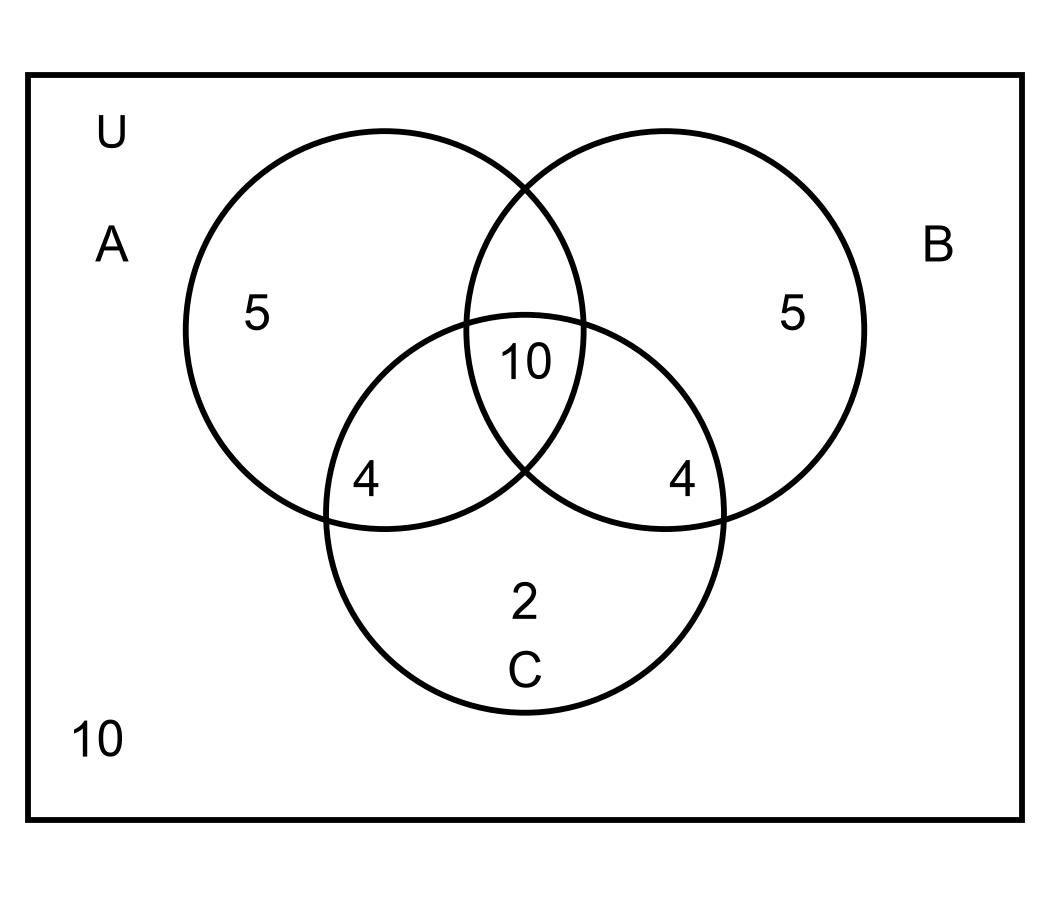
\includegraphics[width=0.38\textwidth]{figures/venn_50_ABC.png}
\end{center}
\step{所以单选物理、化学的人数至多 10 人.}
\step{所以至多选选择物理和化学这两门课程的学生人数至多 $10+10=20$ 人.}
\step{故选 C.}
\solend

\fi

\item 设 $k\geqslant 1,\,k\in\mathbb{N}$，已知集合 $M=\{1,2,3,4,5\}$，若集合 $N_1,N_2,\dots,N_k$ 是集合 $M$ 的 $k$ 个不同非空子集，且 $N_1\cup N_2\cup\dots\cup N_k\neq M$，则 $k$ 的最大值为\mbox{（\quad）.}

\keepwithprev
A. $15$\qquad B. $16$\qquad C. $31$\qquad D. $32$

\ans{A}

\ifanswer
\solbegin
\step{由 $N_1\cup N_2\cup\dots\cup N_k\neq M$ 得所有非空子集的并集缺少集合 $M$ 中至少一个元素.}
\step{假设缺少元素 1，则所有非空子集 $N_i$ 均不含元素 1，即 $N_i$ 是集合 $\{2,3,4,5\}$ 非空子集，集合 $\{2,3,4,5\}$ 的非空子集个数为 $2^4-1=15$，且这些子集 $N_i$ 的并集必不含 1，满足条件.}
\step{假设 $k\geqslant 16$，要满足所有非空子集的并集不等于集合 $M$，必须至少有一个集合 $M$ 中的元素不在任何一个子集中，否则并集就会等于 $M$.}
\step{设这个缺失的元素是 1，那么 $k$ 个非空集都不含元素 1，即每个子集都是集合 $\{2,3,4,5\}$ 的非空子集.}
\step{而集合 $\{2,3,4,5\}$ 只有 $2^4-1=15$ 个不同的非空子集，所以无法从中取出至少 16 个不同的非空子集.}
\step{因此假设不成立，$k$ 必须小于 16.}
\step{所以 $k$ 的最大值为 15，故选 A.}
\solend

\fi

% 注：原卷此题的差集记号是反斜杠 $A\setminus B$（本稿曾误作 $A\vee B$）；$C$ 的集合描述里原卷留了一条
%     待填横线“$x\in A\underline{\quad}B$”（选项按填入的符号分四种情形），本稿曾误作 $\vee\vee$。
%     2026-09-15 回原图核对时已按原卷改回。
\item 对于集合 $A$、$B$，定义 $A\setminus B=\{x\mid x\in A\text{ 且 }x\notin B\}$，则对于集合 $A=\{x\mid x=6n+5,\,n\in\mathbb{N}\}$，$B=\{y\mid y=3m+7,\,m\in\mathbb{N}\}$，$C=\{x\mid x\in A\underline{\hspace{4em}}B\text{ 且 }x<1000\}$，以下说法正确的是\mbox{（\quad）.}

\keepwithprev
A. 若在横线上填入“$\cap$”，则 $C$ 的真子集有 $2^{12}-1$ 个；

B. 若在横线上填入“$\cup$”，则 $C$ 中元素个数大于 250；

C. 若在横线上填入“$\setminus$”，则 $C$ 的非空真子集有 $2^{153}-2$ 个；

% 注：原卷选项 D 作“若在横线上填入“$\cup\complement_{\mathbb N}$”，则 $\complement_{\mathbb N}C$ 中元素个数为 13”；
%     本稿曾把 $\complement_{\mathbb N}$ 抄成 $\varnothing$、把 $\complement_{\mathbb N}C$ 抄成 $C\setminus C$，2026-09-15 回原图核对时已订正。
D. 若在横线上填入“$\cup\complement_{\mathbb{N}}$”，则 $\complement_{\mathbb{N}}C$ 中元素个数为 13.

\ans{B}

\ifanswer
\solbegin
\step{$x=6n+5=3(2n+1)+2$，$y=3m+7=3(m+2)+1$，集合 $A$、$B$ 无公共元素.}
\step{选项 A 中，集合 $C$ 为空集，没有真子集，$A$ 错；}
\step{选项 B 中，由 $6n+5<1000$ 得 $n<165\tfrac{5}{6}$，由 $3m+7<1000$ 得 $m<331$，因此 $C$ 中元素个数为 $166+331=497$，B 正确；}
\step{选项 C 中，$C$ 中元素个数为 166，非空真子集个数为 $2^{166}-2$，C 错；}
% 注：原卷此行作“$\complement_{\mathbb N}C=\complement_{\mathbb N}(A\cup\complement_{\mathbb N}B)
%     =\complement_{\mathbb N}A\cap\complement_{\mathbb N}(\complement_{\mathbb N}B)=\complement_{\mathbb N}A\cap B$，
%     而 $B\subseteq\complement_{\mathbb N}A$”；本稿曾把 $\complement_{\mathbb N}$ 抄成 $C\setminus$，同日已订正。
\step{选项 D 中，$\complement_{\mathbb{N}}C=\complement_{\mathbb{N}}(A\cup\complement_{\mathbb{N}}B)=\complement_{\mathbb{N}}A\cap\complement_{\mathbb{N}}(\complement_{\mathbb{N}}B)=\complement_{\mathbb{N}}A\cap B$，而 $B\subseteq\complement_{\mathbb{N}}A$.}
\step{因此其中元素个数为 331 个，D 错.}
\step{故选 B.}
\solend

\fi
\end{enumerate}

\bigsec{三、解答题}

\begin{enumerate}
\setcounter{enumi}{16}

\item 已知集合 $A=\{x\mid x<-1\text{ 或 }x>4\}$，$B=\{x\mid m+1\leqslant x\leqslant 2m+4\}$.
\begin{enumerate}[label=(\arabic*)]
\item 若 $m=2$，求 $A\cup B$ 和 $\left(\complement_{\R} A\right)\cap B$；
\item 若 $A\cap B=\varnothing$，求 $m$ 的取值范围.
\end{enumerate}

\ans{（1）$A\cup B=\{x\mid x<-1\text{ 或 }x\geqslant 3\}$，$\left(\complement_{\R} A\right)\cap B=\{x\mid 3\leqslant x\leqslant 4\}$；（2）$(-\infty,-3)\cup[-2,0]$}

\ifanswer
\solbegin
\stepm{(1)}{当 $m=2$ 时，集合 $B=\{x\mid 3\leqslant x\leqslant 8\}$.}
\step{又因为 $A=\{x\mid x<-1\text{ 或 }x>4\}$，则 $\complement_{\R}A=\{x\mid -1\leqslant x\leqslant 4\}$，所以 $A\cup B=\{x\mid x<-1\text{ 或 }x\geqslant 3\}$，$\left(\complement_{\R} A\right)\cap B=\{x\mid 3\leqslant x\leqslant 4\}$.}
\stepm{(2)}{因为 $A\cap B=\varnothing$，所以当 $B=\varnothing$ 时，$m+1>2m+4$，解得 $m<-3$ 满足题意；}
\step{当 $B\neq\varnothing$ 时，要满足题意，只需 $\begin{cases}m+1\leqslant 2m+4 \\ m+1\geqslant -1 \\ 2m+4\leqslant 4\end{cases}$，解得 $-2\leqslant m\leqslant 0$.}
\step{综上，实数 $m$ 的范围为 $m<-3$ 或 $-2\leqslant m\leqslant 0$，即 $(-\infty,-3)\cup[-2,0]$.}
\solend

\fi
\ansspace[6]
\item 设集合 $A=\{x\mid x^2+4x=0\}$，$B=\{x\mid x^2+2(a+1)x+a^2-1=0\}$.
\begin{enumerate}[label=(\arabic*)]
\item 写出集合 $A$ 的所有子集；
\item 若 $A\cap B=B$，求实数 $a$ 的取值范围.
\end{enumerate}

\ans{（1）$\{\varnothing,\{0\},\{-4\},\{0,-4\}\}$；（2）$a=1$ 或 $a\leqslant -1$}

\ifanswer
\solbegin
% 注：原卷此行印作“集合 $A$ 的所有子集为 $\varnothing,\{0\},\{-4\},\{0-4\}$”（末项漏逗号、且未加外层花括号）；
%     本稿按规范的列举写法给出，2026-09-15 回原图核对时加注。
\stepm{(1)}{由题意得 $A=\{0,-4\}$，集合 $A$ 的所有子集为 $\varnothing,\{0\},\{-4\},\{0,-4\}$.}
\stepm{(2)}{由 $A\cap B=B$ 得 $B\subseteq A$，所以 $B=\{0\}$ 或 $B=\{-4\}$ 或 $B=\{0,-4\}$ 或 $B=\varnothing$.}
\step{若 $B=\{0\}$ 时，$x^2+2(a+1)x+a^2-1=0$ 有两个相等的根 $0$，则 $\begin{cases}-2(a+1)=0 \\ a^2-1=-4\times(-4)\end{cases}$，解得 $a=-1$.}
\step{若 $B=\{-4\}$ 时，$x^2+2(a+1)x+a^2-1=0$ 有两个相等的根 $-4$，则 $\left\{\begin{matrix}-2(a+1)=-8 \\ a^2-1=-4\times(-4)\end{matrix}\right.$，$a$ 无解.}
\step{若 $B=\{0,-4\}$ 时，$x^2+2(a+1)x+a^2-1=0$ 有两个不相等的根 $0$ 和 $-4$，则 $\begin{cases}-2(a+1)=-4 \\ a^2-1=0\end{cases}$，解得 $a=1$.}
\step{当 $B=\varnothing$ 时，$x^2+2(a+1)x+a^2-1=0$ 无实数根，$\Delta=[2(a+1)]^2-4(a^2-1)=8a+8<0$，得 $a<-1$.}
\step{综上，$a=1$ 或 $a\leqslant -1$.}
\solend

\fi
\ansspace[6]
\item 已知集合 $A=\{x\mid x^2-5x+6=0\}$，$B=\{x\mid mx+1=0\}$，$C=\{x\in\mathbb{N}\mid \sqrt{x}\leqslant 1\}$，且 $A\cup B=A$.
\begin{enumerate}[label=(\arabic*)]
\item 求集合 $M=\{x\mid x\subseteq A\}$ 的真子集的个数；
\item 求实数 $m$ 的值组成的集合；
% 注：原卷本题的定义作“集合 $E=\{x\mid -x\in D,\,2-x^2\notin D\}$”；本稿曾把 $\notin$ 抄成 $\in$
%     （那样 $E=\varnothing$，与答案 $-5$ 冲突），2026-09-15 回原图核对时已订正。
\item 若集合 $D=A\cup C$，定义：集合 $E=\{x\mid -x\in D,\,2-x^2\notin D\}$，求集合 $E$ 中所有元素的和.
\end{enumerate}

\ans{（1）$15$；（2）$\left\{0,-\tfrac{1}{2},-\tfrac{1}{3}\right\}$；（3）$-5$}

\ifanswer
\solbegin
\stepm{(1)}{$A=\{x\mid x^2-5x+6=0\}=\{2,3\}$.}
\step{由 $M=\{x\mid x\subseteq A\}$ 得 $M$ 是 $A$ 的所有子集构成的集合，集合 $A$ 有 2 个元素，故 $A$ 的子集共 $2^2=4$ 个，即 $M$ 含 4 个元素，$M$ 的真子集个数为 $2^4-1=15$.}
\stepm{(2)}{由 (1) 得 $A=\{2,3\}$，集合 $B=\{x\mid mx+1=0\}$.}
\step{由 $A\cup B=A$ 得 $B\subseteq A$，分两种情况：① 当 $m=0$ 时，方程 $mx+1=0$ 无解，$B=\varnothing$，空集是任意集合的子集，符合条件；}
\stepm{②}{当 $m\neq 0$ 时，$B=\{-\tfrac{1}{m}\}$，由 $B\subseteq A$ 得 $-\tfrac{1}{m}=2$ 或 $-\tfrac{1}{m}=3$，解得 $m=-\tfrac{1}{2}$ 或 $m=-\tfrac{1}{3}$.}
\step{实数 $m$ 的取值集合为 $\left\{0,-\tfrac{1}{2},-\tfrac{1}{3}\right\}$.}
\stepm{(3)}{由 (1) 得 $A=\{2,3\}$.}
\step{由 $x\in\mathbb{N}$ 且 $\sqrt{x}\leqslant 1$，得 $x=0$ 或 $x=1$，故 $C=\{0,1\}$.}
\step{所以 $D=A\cup C=\{0,1,2,3\}$.}
\step{由 $-x\in D$ 得 $x$ 的候选值为 $0,-1,-2,-3$.}
\step{由于集合 $E=\{x\mid -x\in D,\,2-x^2\in D\}$，当 $x=0$ 时，$2-x^2=2\in D$，不符合题意；}
\step{当 $x=-1$ 时，$2-x^2=1\in D$，不符合题意；}
\step{当 $x=-2$ 时，$2-x^2=-2\notin D$，符合题意；}
\step{当 $x=-3$ 时，$2-x^2=-7\notin D$，符合题意.}
\step{故 $E=\{-2,-3\}$，所有元素的和为 $-2+(-3)=-5$.}
\solend

\fi
\ansspace[8]
\item 设集合 $M$ 是至少含有两个元素的数集，若 $M$ 中存在两个元素 $x$、$y$ 满足它们的积 $xy\in M$，则称 $M$ 为可积数集.
\begin{enumerate}[label=(\arabic*)]
\item 设集合 $A=\{2,3,5\}$，试判断 $A$ 是否为可积数集？并说明理由；
\item 设集合 $B=\{2,3,4,a\}$，若 $B$ 为可积数集，求实数 $a$ 的取值集合；
\item 设集合 $D=\{x\mid t<x<t+2\}$，若 $D$ 不是可积数集，求实数 $t$ 的取值范围.
\end{enumerate}

% 注：原卷本题【答案】与文末解析的结论都含 $\frac{3}{4}$；本稿曾漏掉 $\frac{3}{4}$
%     （与本稿自己的解析结论不一致），2026-09-15 回原图核对时已订正。
\ans{（1）否；（2）$\left\{0,\tfrac{1}{2},\tfrac{2}{3},\tfrac{3}{4},1,\tfrac{4}{3},\tfrac{3}{2},6,8,12\right\}$；（3）$t\in(-\infty,-2]\cup[2,+\infty)$}

\ifanswer
\solbegin
\stepm{(1)}{因为 $2\times 3=6\notin A$，$2\times 5=10\notin A$，$3\times 5=15\notin A$，所以 $A$ 中任意两个元素的积都不是 $A$ 中的元素，即 $A$ 不是可积数集.}
\stepm{(2)}{若 $B=\{2,3,4,a\}$ 为可积数集，则 $2\times 3=6\in B$，或 $2\times 4=8\in B$ 或 $3\times 4=12\in B$ 或 $2a\in B$ 或 $3a\in B$ 或 $4a\in B$.}
\step{若 $6\in B$，则 $a=6$；}
\step{若 $8\in B$，则 $a=8$；}
\step{若 $12\in B$，则 $a=12$；}
\step{若 $2a\in B$，则 $2a=2$ 或 $2a=3$ 或 $2a=4$ 或 $2a=a$，解得 $a=1$ 或 $a=\tfrac{3}{2}$ 或 $a=2$（舍）或 $a=0$；}
\step{若 $3a\in B$，则 $3a=2$ 或 $3a=3$ 或 $3a=4$ 或 $3a=a$，解得 $a=\tfrac{2}{3}$ 或 $a=1$ 或 $a=\tfrac{4}{3}$ 或 $a=0$；}
\step{若 $4a\in B$，则 $4a=2$ 或 $4a=3$ 或 $4a=4$ 或 $4a=a$，解得 $a=\tfrac{1}{2}$ 或 $a=\tfrac{3}{4}$ 或 $a=1$ 或 $a=0$.}
\step{综上，实数 $a$ 的取值集合为 $\left\{0,\tfrac{1}{2},\tfrac{2}{3},\tfrac{3}{4},1,\tfrac{4}{3},\tfrac{3}{2},6,8,12\right\}$.}
\stepm{(3)}{若 $D=\{x\mid t<x<t+2\}$ 不是可积数集，则 $\forall x,y\in(t,t+2)$，$xy\notin(t,t+2)$.}
\step{当 $t+2\leqslant 0$，即 $t\leqslant -2$ 时，$0\leqslant(t+2)^2<xy<t^2$，此时 $xy\notin D$，满足题意；}
\step{当 $t\geqslant 0$ 时，$0\leqslant t^2<xy<(t+2)^2$，因为 $(t+2)^2>t$，所以若 $xy\notin D$，则 $t^2\geqslant t+2$，即 $t^2-t-2\geqslant 0$，解得 $t\geqslant 2$ 或 $t\leqslant -1$，此时 $t\geqslant 2$ 满足题意；}
% 注：原卷此句作“当 $t<0<t+2$，即 $-2<t<0$ 时，$\exists x=0$，$xy=0\in D$，不满足题意，舍去”；
%     本稿曾把 $\in D$ 抄成 $\notin D$（$-2<t<0$ 时 $0\in(t,t+2)$，确有 $0\in D$），同日已订正。
\step{当 $t<0<t+2$，即 $-2<t<0$ 时，$\exists x=0$，$xy=0\in D$，不满足题意，舍去.}
\step{综上，所求实数 $t$ 的取值范围为 $t\geqslant 2$ 或 $t\leqslant -2$，故 $t\in(-\infty,-2]\cup[2,+\infty)$.}
\solend

\fi
\ansspace[8]
\ansneed{7cm}
\item 已知集合 $A$ 为非空数集，定义：$S=\{x\mid x=a+b,\,a,b\in A\}$，$T=\{x\mid x=|a-b|,a,b\in A\}$（实数 $a$、$b$ 可以相同）.
\begin{enumerate}[label=(\arabic*)]
\item 若集合 $A=\{2,5\}$，直接写出集合 $S$、$T$；
\item 若集合 $A=\{x_1,x_2,x_3,x_4\}$，$x_1<x_2<x_3<x_4$，且 $T=A$，求证：$x_1+x_4=x_3+x_2$；
\item 若集合 $A\subseteq\{x\mid 0\leqslant x\leqslant 2025,\,x\in\mathbb{N}\}$，$S\cap T=\varnothing$，记 $|A|$ 为集合 $A$ 中的元素个数，求 $|A|$ 的最大值.
\end{enumerate}

\ans{（1）$S=\{4,7,10\}$，$T=\{0,3\}$；（2）略；（3）$1350$}

\ifanswer
\solbegin
\stepm{(1)}{$S=\{4,7,10\}$，$T=\{0,3\}$.}
\stepm{(2)}{由集合 $A=\{x_1,x_2,x_3,x_4\}$，$x_1<x_2<x_3<x_4$，则 $T$ 集合的元素在 $0,x_2-x_1,x_3-x_1,x_4-x_1,x_3-x_2,x_4-x_2,x_4-x_3$ 中，且 $0<x_2-x_1<x_3-x_1<x_4-x_1$，$x_3-x_2<x_4-x_2<x_4-x_3$，因为 $A=T$，所以 $A$ 中最大元素 $x_4$ 必在 $T$ 中，而 $x_4-x_1$ 为 7 个元素中的最大者.}
\step{故 $x_4=x_4-x_1$，即 $x_1=0$.}
\step{故 $A=\{0,x_2,x_3,x_4\}$.}
\step{则 $x_3-x_2$、$x_4-x_2$、$x_4-x_3$ 与 $x_2$、$x_3$、$x_4$ 重复.}
\step{而 $0<x_3-x_2<x_3$，故 $x_3-x_2=x_2$，即 $x_3=2x_2$.}
% 注：原卷此句作“而 $0<x_4-x_3<x_4$，故 $x_4-x_3=x_2$ 或 $x_4-x_3=x_3$”；本稿曾把上界写成 $x_3$
%     （那样排除不了 $x_4-x_3=x_3$，与后半句自相矛盾），2026-09-15 回原图核对时已订正。
\step{而 $0<x_4-x_3<x_4$，故 $x_4-x_3=x_2$ 或 $x_4-x_3=x_3$.}
\step{若 $x_4=2x_3=4x_2$，则 $A=\{0,x_2,2x_2,4x_2\}$，$4x_2-x_2=3x_2\notin T$，与题设矛盾.}
\step{故 $x_4-x_3=x_2$，又因为 $x_1=0$，所以 $x_4+x_1=x_3+x_2$.}
% 注：原卷此行作“则 $2a_1<a_1+a_2<a_1+a_3<\cdots<a_1+a_k<a_2+a_k<a_3+a_k<\cdots<a_{k-1}+a_k<2a_k$，
%     所以 $|S|\geqslant 2k-1$，$a_1-a_1<a_2-a_1<a_3-a_1<\cdots<a_k-a_1$，所以 $|T|\geqslant k$”；
%     本稿曾把这个不等式链抄乱（作 $\cdots<a_1+a_k<a_2+a_3<a_k+a_k\leqslant 2a_k$）且把首项写成 $a_i-a_1$，
%     2026-09-15 回原图核对时已订正。
\stepm{(3)}{设 $A=\{a_1,a_2,\dots,a_k\}$ 满足题意，其中 $a_1<a_2<\dots<a_k$，则 $2a_1<a_1+a_2<a_1+a_3<\dots<a_1+a_k<a_2+a_k<a_3+a_k<\dots<a_{k-1}+a_k<2a_k$，所以 $|S|\geqslant 2k-1$，$a_1-a_1<a_2-a_1<a_3-a_1<\dots<a_k-a_1$，所以 $|T|\geqslant k$.}
\step{因为 $S\cap T=\varnothing$，由容斥原理得 $|S\cup T|=|S|+|T|\geqslant 3k-1$.}
\step{$S\cup T$ 中最小的元素为 0，最大的元素为 $2a_k$，$|S\cup T|\leqslant 2a_k+1$，所以 $3k-1\leqslant 2a_k+1\leqslant 2\times 2025+1\,(k\geqslant 1,k\in\mathbb{N})$，即 $3k-1\leqslant 4051$，解得 $k\leqslant 1350\tfrac{2}{3}$.}
\step{实际上 $A=\{676,677,678,\dots,2025\}$ 时满足题意，证明如下：设 $A=\{m,m+1,m+2,\dots,2025\}$，$m\in\mathbb{N}$.}
\step{则 $S=\{2m,2m+1,2m+2,\dots,4050\}$，$T=\{0,1,2,\dots,2025-m\}$.}
\step{由题意得 $2025-m<2m$，即 $m>675$.}
\step{所以 $A=\{676,677,678,\dots,2025\}$ 时满足题意，此时集合 $A$ 中的元素的个数最多.}
\step{综上所述，集合 $A$ 中元素的个数的最大值是 1350.}
\solend

\fi
\ansspace*[10]
\end{enumerate}

\end{document}"
%
% 原始材料是微信公众号图文（“魔都数学加油站”，作者署名“破晓”），正文为 11 张 PNG 页
% （1080×1527）；卷面上的粉色斜水印“魔都数学加油站”属水印，未录入。原文本身就是一份
% **讲评版**——题下直接印出【答案】或【解析】，本稿把这些答案与解析移到答案版，试卷版即
% 一张干净的空卷。
%
% 与原卷的排版差异（均已在 README“说明”中交代）：
%   ① 原文自**第 3 题**起（第 1、2 题未在该文发布），源码里以 \setcounter{enumi}{2} 起编；
%   ② 原卷本就印有分节标题“一、填空题”“二、选择题”“三、解答题”（已在原图上逐页放大
%      核对过），本稿照原卷分节，只把标题改排成全稿统一的“大节标题”样式；
%   ③ 原卷的实数集、整数集符号作正体 $R$（第 7 题）、$Z$（第 11 题），本稿按全稿惯例统一
%      写作 $\R$、$\Z$；
%   ④ 第 14 题【解析】里的 Venn 图取自原卷截图（`figures/venn_50_ABC.png`，4× LANCZOS
%      放大），未用 TikZ 重绘.

\documentclass[a4paper,11pt]{article}
\usepackage{common}

\begin{document}

\examtitlest{2026--2027 学年度交附闵行高一上周练 1}{集合与常用逻辑用语}

\bigsec{一、填空题}

\begin{enumerate}
\setcounter{enumi}{2}

\item 已知集合 $A=\{2,14,x^2+5\}$，$B=\{2,2x\}$，若 $A\cap B=B$，则实数 $x=$ \blankline[2em].

\ans{$7$}

\ifanswer
\solbegin
\step{因为 $A\cap B=B$，所以 $B\subseteq A$，所以 $2x=14$ 或 $x^2+5=2x$.}
\step{$2x=14$ 时，$x=7$，此时 $A=\{2,14,54\}$，$B=\{2,14\}$ 满足题意；}
\step{$x^2+5=2x$ 时，$(x-1)^2+4=0$，无解.}
\step{所以 $x=7$.}
\solend

\fi
\item 设集合 $A=\{y\mid y=x^2-1\}$，$B=\{(x,y)\mid y=x\}$，则 $A\cap B=$ \blankline[2em].

\ans{$\varnothing$}

\item 若集合 $\{0,-1,2a\}=\{a-1,-|a|,a+1\}$，实数 $a$ 的值为 \blankline[2em].

\ans{$\pm 1$}

\ifanswer
\solbegin
\step{令 $A=\{0,-1,2a\}$，$B=\{a-1,-|a|,a+1\}$，因为 $\{0,-1,2a\}=\{a-1,-|a|,a+1\}$，若 $a-1=0$，则 $a=1$，则 $A=\{0,-1,2\}$，$B=\{0,-1,2\}$，满足要求；}
\step{若 $-|a|=0$，则 $a=0$，则 $A=\{0,-1,0\}$，不满足集合元素的互异性；}
\step{若 $a+1=0$，则 $a=-1$，则 $A=\{0,-1,-2\}$，$B=\{0,-1,-2\}$，满足要求.}
\step{故实数 $a$ 的值为 $\pm 1$.}
\solend

\fi
\item 已知全集 $U=(-4,3]$，$A=\{x\in U\mid x^2+2x-8=0\}$，$B=\{x\in U\mid -3<1-2x\leqslant 5\}$，则 $\left(\complement_U B\right)\cap A=$ \blankline[2em].

\ans{$\{2\}$}

\item 已知集合 $A=\{x\mid 1-a\leqslant x\leqslant 1+a,\,a\in\R\}$ 中只有一个整数元素，则实数 $a$ 的取值范围为 \blankline[2em].

\ans{$[0,1)$}

\ifanswer
\solbegin
\step{集合 $A=\{x\mid 1-a\leqslant x\leqslant 1+a,\,a\in\R\}$ 中只有一个整数元素，则 $A\neq\varnothing,\,1-a\leqslant 1+a$，即 $a\geqslant 0$，此时 $1\in A$，故 $\begin{cases}1+a<2 \\ 1-a>0\end{cases}$，解得 $a<1$.}
\step{故 $a\in[0,1)$.}
\solend

\fi
\item 已知全集 $U=\{x\in\mathbb{N}\mid x\leqslant 9\}$，$A\cap B=\{3\}$，$\overline{A}\cap B=\{4,6,8\}$，$A\cap\overline{B}=\{1,5\}$，则 $\overline{A}=$ \blankline[2em].

\ans{$\{0,2,4,6,7,8,9\}$}

\ifanswer
\solbegin
\step{由题意得 $U=\{x\in\mathbb{N}\mid x\leqslant 9\}=\{0,1,2,3,4,5,6,7,8,9\}$，$A\cap B=\{3\}$ 得 $A$、$B$ 中含有元素 $3$；}
\step{$\overline{A}\cap B=\{4,6,8\}$ 得 $B$ 中含有 $4$、$6$、$8$，集合 $A$ 中不含 $4$、$6$、$8$；}
\step{$A\cap\overline{B}=\{1,5\}$ 得 $A$ 含有 $1$、$5$，集合 $B$ 不含 $1$、$5$.}
\step{对于 $0$，假设集合 $A$ 中含有 $0$，由 $A\cap B=\{3\}$ 得 $B$ 不含 $0$，则 $A\cap\overline{B}$ 必含元素 $0$，与 $A\cap\overline{B}=\{1,5\}$ 矛盾.}
\step{同理可得集合 $A$ 中不含元素 $2$、$7$、$9$.}
\step{综上所述，$A=\{1,3,5\}$.}
\step{故 $\overline{A}=\{0,2,4,6,7,8,9\}$.}
\solend

\fi
\item 已知一个有四个数字元素的集合 $S$，$S$ 的所有子集的元素和（空集的元素和认为是 0）的总和为 16208，则 $S$ 的元素之和等于 \blankline[2em].

\ans{$2026$}

\ifanswer
\solbegin
\step{设 $S=\{a_1,a_2,a_3,a_4\}$，$S$ 的每个元素在所有子集中均出现 $2^3$ 次，故 $(a_1+a_2+a_3+a_4)\cdot 2^3=16208$，所以 $a_1+a_2+a_3+a_4=2026$，故 $S$ 的元素之和等于 2026.}
\solend

\fi
\item 已知集合 $M=\{x\in\mathbb{N}\mid 1\leqslant x\leqslant 12\}$，集合 $A_1$、$A_2$、$A_3$ 满足：① 每个集合都恰有 4 个元素；② $A_1\cup A_2\cup A_3=M$. 集合 $A_i\,(i=1,2,3)$ 中元素的最大值与最小值之和称为集合 $A_i$ 的特征数，记为 $X_i\,(i=1,2,3)$，则 $X_1+X_2+X_3$ 的最大值与最小值的积为 \blankline[2em].

\ans{$1485$}

\ifanswer
\solbegin
\step{集合 $M=\{x\in\mathbb{N}\mid 1\leqslant x\leqslant 12\}$ 中最小值为 1，最大值为 12.}
% 注：原卷此处印作“则 $A_1=13$”（原卷笔误，按上下文应为 $X_1=13$），本稿按 $X_1$ 规范，2026-09-15 回原图核对时加注。
\stepm{①}{若使 $X_1+X_2+X_3$ 取得最大值，不妨设 $A_1=\{1,2,3,12\}$，则 $X_1=13$，则剩余的数中最小值是 4，最大值是 11，令 $A_2=\{4,5,6,11\}$，则 $X_2=15$，则 $A_3=\{7,8,9,10\}$，$X_3=17$，则 $X_1+X_2+X_3$ 的最大值为 $13+15+17=45$；}
\stepm{②}{若使 $X_1+X_2+X_3$ 取得最小值，则 $A_1=\{1,4,5,6\}$，则 $X_1=7$，令 $A_2=\{2,7,8,9\}$，则 $X_2=11$，则 $A_3=\{3,10,11,12\}$，$X_3=15$，则此时 $X_1+X_2+X_3$ 的最小值为 $7+11+15=33$.}
\step{故 $X_1+X_2+X_3$ 的最大值与最小值的积为 $45\times 33=1485$.}
\solend

\fi
\item 对于集合 $M=\{a\mid a=x^2-y^2,\,x\in\Z,\,y\in\Z\}$，给出如下三个结论：

① 如果 $P=\{b\mid b=2n+1,\,n\in\Z\}$，那么 $P\subseteq M$；

% 注：原卷此条作“如果 $c=4n+2$，$n\in\Z$，那么 $c\notin M$”；本稿曾把 $\notin$ 抄成 $\in$
%     （那样②为假，与本卷答案 ①②③ 冲突），2026-09-15 回原图核对时已订正。
② 如果 $c=4n+2$，$n\in\Z$，那么 $c\notin M$；

③ 如果 $a_1\in M$，$a_2\in M$，那么 $a_1a_2\in M$. 其中正确结论的序号是 \blankline[2em].

\ans{①②③}

\ifanswer
\solbegin
\stepm{①}{由已知 $b=2n+1,\,n\in\Z$，则恒有 $2n+1=(n+1)^2-n^2,\,n\in\Z$，所以 $2n+1\in M$，所以 $P\subseteq M$，所以①正确；}
\stepm{②}{元素 $c=4n+2,\,n\in\Z$，若 $4n+2\in M$，则存在 $x$、$y\in\Z$ 使得 $x^2-y^2=4n+2$，所以 $4n+2=(x+y)(x-y)$，则 $x+y$ 与 $x-y$ 同奇或同偶.}
\step{若 $x+y$ 与 $x-y$ 都是奇数，则 $(x+y)(x-y)$ 为奇数，而 $4n+2$ 是偶数；}
\step{若 $x+y$ 和 $x-y$ 都是偶数，则 $(x+y)(x-y)$ 能被 4 整除，而 $4n+2$ 不能被 4 整除.}
\step{所以 $4n+2\notin M$，即 $c\notin M$，故②正确；}
\stepm{③}{因为 $a_1$、$a_2\in M$，则 $a_1a_2$ 还是整数，所以 $a_1a_2\in M$，故③正确.}
\step{故正确的是①②③.}
\solend

\fi
\item 用 $C(A)$ 表示非空集合 $A$ 中的元素的个数，定义 $A*B=|C(A)-C(B)|$，若 $A=\{x\mid x^2-2024x-2025=0\}$，$B=\{x\mid (2x^2+ax)(x^2+2ax+6)=0\}$，若 $A*B=1$，则 $a$ 的所有可能取值构成集合 $M$，则 $C(M)=$ \blankline[2em].

\ans{$5$}

\ifanswer
\solbegin
\step{$x^2-2024x-2025=0$ 得 $x=2025$ 或 $x=-1$，即 $C(A)=2$，因为 $A*B=|C(A)-C(B)|=1$，所以 $C(B)=3$ 或 $C(B)=1$.}
\step{方程 $(2x^2+ax)(x^2+2ax+6)=0$ 化为 $x(2x+a)(x^2+2ax+6)=0$.}
\step{当 $a=0$ 时，方程化为 $2x^3(x^2+6)=0$，解得 $x=0$，所以 $B=\{0\}$，$C(B)=1$，符合题意.}
\step{当 $a\neq 0$ 时，方程化为 $x=0$ 或 $x=-\tfrac{a}{2}$ 或 $x^2+2ax+6=0$.}
\step{因为 $0\neq -\tfrac{a}{2}$，$C(B)\neq 1$，故只有 $C(B)=3$.}
\step{故 $x^2+2ax+6=0$ 有两个相等的非零实数根，所以 $\Delta=4a^2-4\times 6=0$，解得 $a=\pm\sqrt{6}$，符合题意.}
\step{当 $x^2+2ax+6=0$ 有两个不相等实根，设 $x_1$、$x_2$，若 $x_1=-\tfrac{a}{2}$，由韦达定理得 $\begin{cases}x_1+x_2=-2a \\ x_1x_2=6\end{cases}$，% 注：原卷作“得 $x_2=-\frac{3a}{2}$”（由 $x_1+x_2=-2a$、$x_1=-\frac{a}{2}$ 得 $x_2=-\frac{3a}{2}$）；
%     本稿曾漏掉负号，2026-09-15 回原图核对时已订正。
得 $x_2=-\tfrac{3a}{2}$，$-\tfrac{a}{2}\cdot(-\tfrac{3a}{2})=\tfrac{3a^2}{4}=6$，解得 $a=\pm 2\sqrt{2}$，符合题意.}
\step{综上所述，$M=\{0,\sqrt{6},-\sqrt{6},2\sqrt{2},-2\sqrt{2}\}$，所以 $C(M)=5$.}
\solend

\fi
\end{enumerate}

\bigsec{二、选择题}

\begin{enumerate}
\setcounter{enumi}{12}

\item 已知集合 $A=\{1,2,3,4,5\}$，$B=\{x\mid \tfrac{x-1}{2}\in\Z,\,x\in A\}$，则集合 $B$ 的真子集个数为\mbox{（\quad）.}

\keepwithprev
A. $3$\qquad B. $5$\qquad C. $7$\qquad D. $15$

\ans{C}

\ifanswer
\solbegin
\step{已知集合 $A=\{1,2,3,4,5\}$，$B=\{x\mid\tfrac{x-1}{2}\in\Z,\,x\in A\}$.}
\step{因为 $\tfrac{x-1}{2}\in\Z$，所以 $x$ 为奇数，所以 $B=\{1,3,5\}$.}
\step{所以集合 $B$ 中有 3 个元素，所以集合 $B$ 的真子集个数为 $2^3-1=7$.}
\step{故选 C.}
\solend

\fi

\item 高一二班共有学生 50 人，每名学生要从物理、化学、生物、历史、地理、政治这六门课程中选择三门课程进行学习. 已知选择物理、化学、生物的学生各有至少 20 人，这三门课程都不选的有 10 人，这三门课程都选的有 10 人，在这三门课程中选择任意两门课程的都至少有 14 人，物理、化学只选一科的学生都至少 5 人，那么选择物理和化学这两门课程的学生人数至多\mbox{（\quad）.}

\keepwithprev
A. $18$\qquad B. $19$\qquad C. $20$\qquad D. $21$

\ans{C}

\ifanswer
\solbegin
\step{可以把学生 50 人看作一个集合 $U$，选择物理的人数组成集合 $A$，选择化学的人数组成集合 $B$，选择生物的人数组成集合 $C$.}
\step{要使选择物理和化学这两门课程的学生人数最多，除这三门课程都不选的有 10 人，这三门课程都选的有 10 人，则其他科选择人数均为最少，因为物理、化学只选一科的学生都至少 5 人，即得到单选物理的最少 5 人，单选化学的最少 5 人.}
\step{因为在这三门课程中选择任意两门课程的都至少有 14 人，单选化学、生物的最少 4 人，单选物理、生物的最少 4 人.}
\step{因为选择物理、化学、生物的学生各有至少 20 人，所以单选生物的最少 2 人.}
\step{以上人数最少 30 人，可作出如图所示的韦恩图：}
% 注：原卷此处印有一张韦恩图（三个圆 $A$、$B$、$C$，$A$ 独有 5、$B$ 独有 5、三集合公共 10、
%     $A\cap C$ 独有 4、$B\cap C$ 独有 4、$C$ 独有 2、三集合之外 10）；本稿此前漏排此图而正文仍作
%     “如图”，2026-09-15 回原图核对时按原卷截图补入（见 figures/venn_50_ABC.png）。
\begin{center}
% 插图取自原卷截图（裁去截图残影后 4× LANCZOS 放大），不用 TikZ 手绘
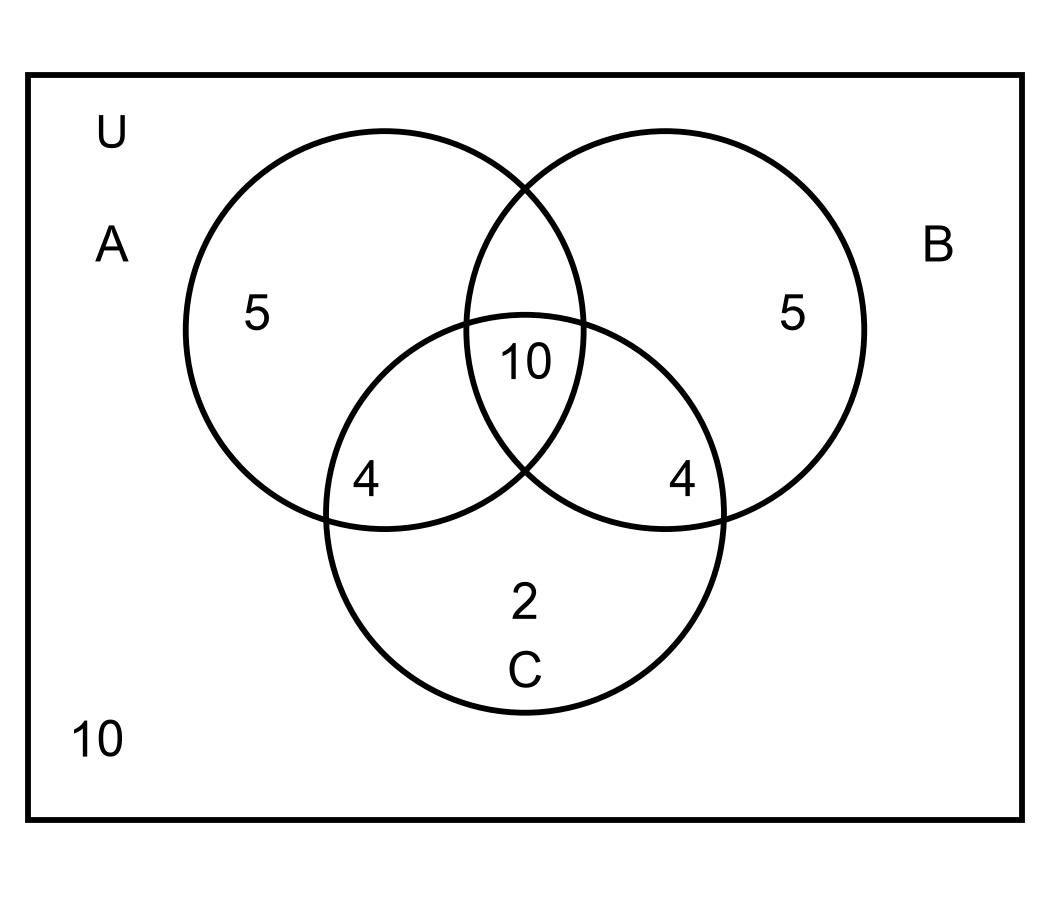
\includegraphics[width=0.38\textwidth]{figures/venn_50_ABC.png}
\end{center}
\step{所以单选物理、化学的人数至多 10 人.}
\step{所以至多选选择物理和化学这两门课程的学生人数至多 $10+10=20$ 人.}
\step{故选 C.}
\solend

\fi

\item 设 $k\geqslant 1,\,k\in\mathbb{N}$，已知集合 $M=\{1,2,3,4,5\}$，若集合 $N_1,N_2,\dots,N_k$ 是集合 $M$ 的 $k$ 个不同非空子集，且 $N_1\cup N_2\cup\dots\cup N_k\neq M$，则 $k$ 的最大值为\mbox{（\quad）.}

\keepwithprev
A. $15$\qquad B. $16$\qquad C. $31$\qquad D. $32$

\ans{A}

\ifanswer
\solbegin
\step{由 $N_1\cup N_2\cup\dots\cup N_k\neq M$ 得所有非空子集的并集缺少集合 $M$ 中至少一个元素.}
\step{假设缺少元素 1，则所有非空子集 $N_i$ 均不含元素 1，即 $N_i$ 是集合 $\{2,3,4,5\}$ 非空子集，集合 $\{2,3,4,5\}$ 的非空子集个数为 $2^4-1=15$，且这些子集 $N_i$ 的并集必不含 1，满足条件.}
\step{假设 $k\geqslant 16$，要满足所有非空子集的并集不等于集合 $M$，必须至少有一个集合 $M$ 中的元素不在任何一个子集中，否则并集就会等于 $M$.}
\step{设这个缺失的元素是 1，那么 $k$ 个非空集都不含元素 1，即每个子集都是集合 $\{2,3,4,5\}$ 的非空子集.}
\step{而集合 $\{2,3,4,5\}$ 只有 $2^4-1=15$ 个不同的非空子集，所以无法从中取出至少 16 个不同的非空子集.}
\step{因此假设不成立，$k$ 必须小于 16.}
\step{所以 $k$ 的最大值为 15，故选 A.}
\solend

\fi

% 注：原卷此题的差集记号是反斜杠 $A\setminus B$（本稿曾误作 $A\vee B$）；$C$ 的集合描述里原卷留了一条
%     待填横线“$x\in A\underline{\quad}B$”（选项按填入的符号分四种情形），本稿曾误作 $\vee\vee$。
%     2026-09-15 回原图核对时已按原卷改回。
\item 对于集合 $A$、$B$，定义 $A\setminus B=\{x\mid x\in A\text{ 且 }x\notin B\}$，则对于集合 $A=\{x\mid x=6n+5,\,n\in\mathbb{N}\}$，$B=\{y\mid y=3m+7,\,m\in\mathbb{N}\}$，$C=\{x\mid x\in A\underline{\hspace{4em}}B\text{ 且 }x<1000\}$，以下说法正确的是\mbox{（\quad）.}

\keepwithprev
A. 若在横线上填入“$\cap$”，则 $C$ 的真子集有 $2^{12}-1$ 个；

B. 若在横线上填入“$\cup$”，则 $C$ 中元素个数大于 250；

C. 若在横线上填入“$\setminus$”，则 $C$ 的非空真子集有 $2^{153}-2$ 个；

% 注：原卷选项 D 作“若在横线上填入“$\cup\complement_{\mathbb N}$”，则 $\complement_{\mathbb N}C$ 中元素个数为 13”；
%     本稿曾把 $\complement_{\mathbb N}$ 抄成 $\varnothing$、把 $\complement_{\mathbb N}C$ 抄成 $C\setminus C$，2026-09-15 回原图核对时已订正。
D. 若在横线上填入“$\cup\complement_{\mathbb{N}}$”，则 $\complement_{\mathbb{N}}C$ 中元素个数为 13.

\ans{B}

\ifanswer
\solbegin
\step{$x=6n+5=3(2n+1)+2$，$y=3m+7=3(m+2)+1$，集合 $A$、$B$ 无公共元素.}
\step{选项 A 中，集合 $C$ 为空集，没有真子集，$A$ 错；}
\step{选项 B 中，由 $6n+5<1000$ 得 $n<165\tfrac{5}{6}$，由 $3m+7<1000$ 得 $m<331$，因此 $C$ 中元素个数为 $166+331=497$，B 正确；}
\step{选项 C 中，$C$ 中元素个数为 166，非空真子集个数为 $2^{166}-2$，C 错；}
% 注：原卷此行作“$\complement_{\mathbb N}C=\complement_{\mathbb N}(A\cup\complement_{\mathbb N}B)
%     =\complement_{\mathbb N}A\cap\complement_{\mathbb N}(\complement_{\mathbb N}B)=\complement_{\mathbb N}A\cap B$，
%     而 $B\subseteq\complement_{\mathbb N}A$”；本稿曾把 $\complement_{\mathbb N}$ 抄成 $C\setminus$，同日已订正。
\step{选项 D 中，$\complement_{\mathbb{N}}C=\complement_{\mathbb{N}}(A\cup\complement_{\mathbb{N}}B)=\complement_{\mathbb{N}}A\cap\complement_{\mathbb{N}}(\complement_{\mathbb{N}}B)=\complement_{\mathbb{N}}A\cap B$，而 $B\subseteq\complement_{\mathbb{N}}A$.}
\step{因此其中元素个数为 331 个，D 错.}
\step{故选 B.}
\solend

\fi
\end{enumerate}

\bigsec{三、解答题}

\begin{enumerate}
\setcounter{enumi}{16}

\item 已知集合 $A=\{x\mid x<-1\text{ 或 }x>4\}$，$B=\{x\mid m+1\leqslant x\leqslant 2m+4\}$.
\begin{enumerate}[label=(\arabic*)]
\item 若 $m=2$，求 $A\cup B$ 和 $\left(\complement_{\R} A\right)\cap B$；
\item 若 $A\cap B=\varnothing$，求 $m$ 的取值范围.
\end{enumerate}

\ans{（1）$A\cup B=\{x\mid x<-1\text{ 或 }x\geqslant 3\}$，$\left(\complement_{\R} A\right)\cap B=\{x\mid 3\leqslant x\leqslant 4\}$；（2）$(-\infty,-3)\cup[-2,0]$}

\ifanswer
\solbegin
\stepm{(1)}{当 $m=2$ 时，集合 $B=\{x\mid 3\leqslant x\leqslant 8\}$.}
\step{又因为 $A=\{x\mid x<-1\text{ 或 }x>4\}$，则 $\complement_{\R}A=\{x\mid -1\leqslant x\leqslant 4\}$，所以 $A\cup B=\{x\mid x<-1\text{ 或 }x\geqslant 3\}$，$\left(\complement_{\R} A\right)\cap B=\{x\mid 3\leqslant x\leqslant 4\}$.}
\stepm{(2)}{因为 $A\cap B=\varnothing$，所以当 $B=\varnothing$ 时，$m+1>2m+4$，解得 $m<-3$ 满足题意；}
\step{当 $B\neq\varnothing$ 时，要满足题意，只需 $\begin{cases}m+1\leqslant 2m+4 \\ m+1\geqslant -1 \\ 2m+4\leqslant 4\end{cases}$，解得 $-2\leqslant m\leqslant 0$.}
\step{综上，实数 $m$ 的范围为 $m<-3$ 或 $-2\leqslant m\leqslant 0$，即 $(-\infty,-3)\cup[-2,0]$.}
\solend

\fi
\ansspace[6]
\item 设集合 $A=\{x\mid x^2+4x=0\}$，$B=\{x\mid x^2+2(a+1)x+a^2-1=0\}$.
\begin{enumerate}[label=(\arabic*)]
\item 写出集合 $A$ 的所有子集；
\item 若 $A\cap B=B$，求实数 $a$ 的取值范围.
\end{enumerate}

\ans{（1）$\{\varnothing,\{0\},\{-4\},\{0,-4\}\}$；（2）$a=1$ 或 $a\leqslant -1$}

\ifanswer
\solbegin
% 注：原卷此行印作“集合 $A$ 的所有子集为 $\varnothing,\{0\},\{-4\},\{0-4\}$”（末项漏逗号、且未加外层花括号）；
%     本稿按规范的列举写法给出，2026-09-15 回原图核对时加注。
\stepm{(1)}{由题意得 $A=\{0,-4\}$，集合 $A$ 的所有子集为 $\varnothing,\{0\},\{-4\},\{0,-4\}$.}
\stepm{(2)}{由 $A\cap B=B$ 得 $B\subseteq A$，所以 $B=\{0\}$ 或 $B=\{-4\}$ 或 $B=\{0,-4\}$ 或 $B=\varnothing$.}
\step{若 $B=\{0\}$ 时，$x^2+2(a+1)x+a^2-1=0$ 有两个相等的根 $0$，则 $\begin{cases}-2(a+1)=0 \\ a^2-1=-4\times(-4)\end{cases}$，解得 $a=-1$.}
\step{若 $B=\{-4\}$ 时，$x^2+2(a+1)x+a^2-1=0$ 有两个相等的根 $-4$，则 $\left\{\begin{matrix}-2(a+1)=-8 \\ a^2-1=-4\times(-4)\end{matrix}\right.$，$a$ 无解.}
\step{若 $B=\{0,-4\}$ 时，$x^2+2(a+1)x+a^2-1=0$ 有两个不相等的根 $0$ 和 $-4$，则 $\begin{cases}-2(a+1)=-4 \\ a^2-1=0\end{cases}$，解得 $a=1$.}
\step{当 $B=\varnothing$ 时，$x^2+2(a+1)x+a^2-1=0$ 无实数根，$\Delta=[2(a+1)]^2-4(a^2-1)=8a+8<0$，得 $a<-1$.}
\step{综上，$a=1$ 或 $a\leqslant -1$.}
\solend

\fi
\ansspace[6]
\item 已知集合 $A=\{x\mid x^2-5x+6=0\}$，$B=\{x\mid mx+1=0\}$，$C=\{x\in\mathbb{N}\mid \sqrt{x}\leqslant 1\}$，且 $A\cup B=A$.
\begin{enumerate}[label=(\arabic*)]
\item 求集合 $M=\{x\mid x\subseteq A\}$ 的真子集的个数；
\item 求实数 $m$ 的值组成的集合；
% 注：原卷本题的定义作“集合 $E=\{x\mid -x\in D,\,2-x^2\notin D\}$”；本稿曾把 $\notin$ 抄成 $\in$
%     （那样 $E=\varnothing$，与答案 $-5$ 冲突），2026-09-15 回原图核对时已订正。
\item 若集合 $D=A\cup C$，定义：集合 $E=\{x\mid -x\in D,\,2-x^2\notin D\}$，求集合 $E$ 中所有元素的和.
\end{enumerate}

\ans{（1）$15$；（2）$\left\{0,-\tfrac{1}{2},-\tfrac{1}{3}\right\}$；（3）$-5$}

\ifanswer
\solbegin
\stepm{(1)}{$A=\{x\mid x^2-5x+6=0\}=\{2,3\}$.}
\step{由 $M=\{x\mid x\subseteq A\}$ 得 $M$ 是 $A$ 的所有子集构成的集合，集合 $A$ 有 2 个元素，故 $A$ 的子集共 $2^2=4$ 个，即 $M$ 含 4 个元素，$M$ 的真子集个数为 $2^4-1=15$.}
\stepm{(2)}{由 (1) 得 $A=\{2,3\}$，集合 $B=\{x\mid mx+1=0\}$.}
\step{由 $A\cup B=A$ 得 $B\subseteq A$，分两种情况：① 当 $m=0$ 时，方程 $mx+1=0$ 无解，$B=\varnothing$，空集是任意集合的子集，符合条件；}
\stepm{②}{当 $m\neq 0$ 时，$B=\{-\tfrac{1}{m}\}$，由 $B\subseteq A$ 得 $-\tfrac{1}{m}=2$ 或 $-\tfrac{1}{m}=3$，解得 $m=-\tfrac{1}{2}$ 或 $m=-\tfrac{1}{3}$.}
\step{实数 $m$ 的取值集合为 $\left\{0,-\tfrac{1}{2},-\tfrac{1}{3}\right\}$.}
\stepm{(3)}{由 (1) 得 $A=\{2,3\}$.}
\step{由 $x\in\mathbb{N}$ 且 $\sqrt{x}\leqslant 1$，得 $x=0$ 或 $x=1$，故 $C=\{0,1\}$.}
\step{所以 $D=A\cup C=\{0,1,2,3\}$.}
\step{由 $-x\in D$ 得 $x$ 的候选值为 $0,-1,-2,-3$.}
\step{由于集合 $E=\{x\mid -x\in D,\,2-x^2\in D\}$，当 $x=0$ 时，$2-x^2=2\in D$，不符合题意；}
\step{当 $x=-1$ 时，$2-x^2=1\in D$，不符合题意；}
\step{当 $x=-2$ 时，$2-x^2=-2\notin D$，符合题意；}
\step{当 $x=-3$ 时，$2-x^2=-7\notin D$，符合题意.}
\step{故 $E=\{-2,-3\}$，所有元素的和为 $-2+(-3)=-5$.}
\solend

\fi
\ansspace[8]
\item 设集合 $M$ 是至少含有两个元素的数集，若 $M$ 中存在两个元素 $x$、$y$ 满足它们的积 $xy\in M$，则称 $M$ 为可积数集.
\begin{enumerate}[label=(\arabic*)]
\item 设集合 $A=\{2,3,5\}$，试判断 $A$ 是否为可积数集？并说明理由；
\item 设集合 $B=\{2,3,4,a\}$，若 $B$ 为可积数集，求实数 $a$ 的取值集合；
\item 设集合 $D=\{x\mid t<x<t+2\}$，若 $D$ 不是可积数集，求实数 $t$ 的取值范围.
\end{enumerate}

% 注：原卷本题【答案】与文末解析的结论都含 $\frac{3}{4}$；本稿曾漏掉 $\frac{3}{4}$
%     （与本稿自己的解析结论不一致），2026-09-15 回原图核对时已订正。
\ans{（1）否；（2）$\left\{0,\tfrac{1}{2},\tfrac{2}{3},\tfrac{3}{4},1,\tfrac{4}{3},\tfrac{3}{2},6,8,12\right\}$；（3）$t\in(-\infty,-2]\cup[2,+\infty)$}

\ifanswer
\solbegin
\stepm{(1)}{因为 $2\times 3=6\notin A$，$2\times 5=10\notin A$，$3\times 5=15\notin A$，所以 $A$ 中任意两个元素的积都不是 $A$ 中的元素，即 $A$ 不是可积数集.}
\stepm{(2)}{若 $B=\{2,3,4,a\}$ 为可积数集，则 $2\times 3=6\in B$，或 $2\times 4=8\in B$ 或 $3\times 4=12\in B$ 或 $2a\in B$ 或 $3a\in B$ 或 $4a\in B$.}
\step{若 $6\in B$，则 $a=6$；}
\step{若 $8\in B$，则 $a=8$；}
\step{若 $12\in B$，则 $a=12$；}
\step{若 $2a\in B$，则 $2a=2$ 或 $2a=3$ 或 $2a=4$ 或 $2a=a$，解得 $a=1$ 或 $a=\tfrac{3}{2}$ 或 $a=2$（舍）或 $a=0$；}
\step{若 $3a\in B$，则 $3a=2$ 或 $3a=3$ 或 $3a=4$ 或 $3a=a$，解得 $a=\tfrac{2}{3}$ 或 $a=1$ 或 $a=\tfrac{4}{3}$ 或 $a=0$；}
\step{若 $4a\in B$，则 $4a=2$ 或 $4a=3$ 或 $4a=4$ 或 $4a=a$，解得 $a=\tfrac{1}{2}$ 或 $a=\tfrac{3}{4}$ 或 $a=1$ 或 $a=0$.}
\step{综上，实数 $a$ 的取值集合为 $\left\{0,\tfrac{1}{2},\tfrac{2}{3},\tfrac{3}{4},1,\tfrac{4}{3},\tfrac{3}{2},6,8,12\right\}$.}
\stepm{(3)}{若 $D=\{x\mid t<x<t+2\}$ 不是可积数集，则 $\forall x,y\in(t,t+2)$，$xy\notin(t,t+2)$.}
\step{当 $t+2\leqslant 0$，即 $t\leqslant -2$ 时，$0\leqslant(t+2)^2<xy<t^2$，此时 $xy\notin D$，满足题意；}
\step{当 $t\geqslant 0$ 时，$0\leqslant t^2<xy<(t+2)^2$，因为 $(t+2)^2>t$，所以若 $xy\notin D$，则 $t^2\geqslant t+2$，即 $t^2-t-2\geqslant 0$，解得 $t\geqslant 2$ 或 $t\leqslant -1$，此时 $t\geqslant 2$ 满足题意；}
% 注：原卷此句作“当 $t<0<t+2$，即 $-2<t<0$ 时，$\exists x=0$，$xy=0\in D$，不满足题意，舍去”；
%     本稿曾把 $\in D$ 抄成 $\notin D$（$-2<t<0$ 时 $0\in(t,t+2)$，确有 $0\in D$），同日已订正。
\step{当 $t<0<t+2$，即 $-2<t<0$ 时，$\exists x=0$，$xy=0\in D$，不满足题意，舍去.}
\step{综上，所求实数 $t$ 的取值范围为 $t\geqslant 2$ 或 $t\leqslant -2$，故 $t\in(-\infty,-2]\cup[2,+\infty)$.}
\solend

\fi
\ansspace[8]
\ansneed{7cm}
\item 已知集合 $A$ 为非空数集，定义：$S=\{x\mid x=a+b,\,a,b\in A\}$，$T=\{x\mid x=|a-b|,a,b\in A\}$（实数 $a$、$b$ 可以相同）.
\begin{enumerate}[label=(\arabic*)]
\item 若集合 $A=\{2,5\}$，直接写出集合 $S$、$T$；
\item 若集合 $A=\{x_1,x_2,x_3,x_4\}$，$x_1<x_2<x_3<x_4$，且 $T=A$，求证：$x_1+x_4=x_3+x_2$；
\item 若集合 $A\subseteq\{x\mid 0\leqslant x\leqslant 2025,\,x\in\mathbb{N}\}$，$S\cap T=\varnothing$，记 $|A|$ 为集合 $A$ 中的元素个数，求 $|A|$ 的最大值.
\end{enumerate}

\ans{（1）$S=\{4,7,10\}$，$T=\{0,3\}$；（2）略；（3）$1350$}

\ifanswer
\solbegin
\stepm{(1)}{$S=\{4,7,10\}$，$T=\{0,3\}$.}
\stepm{(2)}{由集合 $A=\{x_1,x_2,x_3,x_4\}$，$x_1<x_2<x_3<x_4$，则 $T$ 集合的元素在 $0,x_2-x_1,x_3-x_1,x_4-x_1,x_3-x_2,x_4-x_2,x_4-x_3$ 中，且 $0<x_2-x_1<x_3-x_1<x_4-x_1$，$x_3-x_2<x_4-x_2<x_4-x_3$，因为 $A=T$，所以 $A$ 中最大元素 $x_4$ 必在 $T$ 中，而 $x_4-x_1$ 为 7 个元素中的最大者.}
\step{故 $x_4=x_4-x_1$，即 $x_1=0$.}
\step{故 $A=\{0,x_2,x_3,x_4\}$.}
\step{则 $x_3-x_2$、$x_4-x_2$、$x_4-x_3$ 与 $x_2$、$x_3$、$x_4$ 重复.}
\step{而 $0<x_3-x_2<x_3$，故 $x_3-x_2=x_2$，即 $x_3=2x_2$.}
% 注：原卷此句作“而 $0<x_4-x_3<x_4$，故 $x_4-x_3=x_2$ 或 $x_4-x_3=x_3$”；本稿曾把上界写成 $x_3$
%     （那样排除不了 $x_4-x_3=x_3$，与后半句自相矛盾），2026-09-15 回原图核对时已订正。
\step{而 $0<x_4-x_3<x_4$，故 $x_4-x_3=x_2$ 或 $x_4-x_3=x_3$.}
\step{若 $x_4=2x_3=4x_2$，则 $A=\{0,x_2,2x_2,4x_2\}$，$4x_2-x_2=3x_2\notin T$，与题设矛盾.}
\step{故 $x_4-x_3=x_2$，又因为 $x_1=0$，所以 $x_4+x_1=x_3+x_2$.}
% 注：原卷此行作“则 $2a_1<a_1+a_2<a_1+a_3<\cdots<a_1+a_k<a_2+a_k<a_3+a_k<\cdots<a_{k-1}+a_k<2a_k$，
%     所以 $|S|\geqslant 2k-1$，$a_1-a_1<a_2-a_1<a_3-a_1<\cdots<a_k-a_1$，所以 $|T|\geqslant k$”；
%     本稿曾把这个不等式链抄乱（作 $\cdots<a_1+a_k<a_2+a_3<a_k+a_k\leqslant 2a_k$）且把首项写成 $a_i-a_1$，
%     2026-09-15 回原图核对时已订正。
\stepm{(3)}{设 $A=\{a_1,a_2,\dots,a_k\}$ 满足题意，其中 $a_1<a_2<\dots<a_k$，则 $2a_1<a_1+a_2<a_1+a_3<\dots<a_1+a_k<a_2+a_k<a_3+a_k<\dots<a_{k-1}+a_k<2a_k$，所以 $|S|\geqslant 2k-1$，$a_1-a_1<a_2-a_1<a_3-a_1<\dots<a_k-a_1$，所以 $|T|\geqslant k$.}
\step{因为 $S\cap T=\varnothing$，由容斥原理得 $|S\cup T|=|S|+|T|\geqslant 3k-1$.}
\step{$S\cup T$ 中最小的元素为 0，最大的元素为 $2a_k$，$|S\cup T|\leqslant 2a_k+1$，所以 $3k-1\leqslant 2a_k+1\leqslant 2\times 2025+1\,(k\geqslant 1,k\in\mathbb{N})$，即 $3k-1\leqslant 4051$，解得 $k\leqslant 1350\tfrac{2}{3}$.}
\step{实际上 $A=\{676,677,678,\dots,2025\}$ 时满足题意，证明如下：设 $A=\{m,m+1,m+2,\dots,2025\}$，$m\in\mathbb{N}$.}
\step{则 $S=\{2m,2m+1,2m+2,\dots,4050\}$，$T=\{0,1,2,\dots,2025-m\}$.}
\step{由题意得 $2025-m<2m$，即 $m>675$.}
\step{所以 $A=\{676,677,678,\dots,2025\}$ 时满足题意，此时集合 $A$ 中的元素的个数最多.}
\step{综上所述，集合 $A$ 中元素的个数的最大值是 1350.}
\solend

\fi
\ansspace*[10]
\end{enumerate}

\end{document}